%---------------------------------------------------
% University of Sussex thesis template
% Last Edit by Fabrizio Miano, Oct 2017
%---------------------------------------------------
%!TeX root = ../main.tex
\documentclass[a4paper,11pt,oneside]{memoir}
\usepackage[british]{babel}


%---------------------------------------------------
% DOCUMENT VARIABLES
% Fill in the lines below to enter your information into the thesis template
% Each of the commands can be cited anywhere in the thesis
%---------------------------------------------------
\newcommand{\myTitle}{Photons illuminating the unknown}
%use surd as ASCII sqrt symbol in case needed and fix title separately

\newcommand{\mySubtitle}{Search for high-mass resonances in \(\gamma\)+jet final states}
% Is SUSY in the tau corner? A tale of triggers and tau decays From triggering to taus
%\newcommand{\mySubtitle}{the adventure begins with staus\xspace}
\newcommand{\myDegree}{Doctor of Philosophy \xspace}
\newcommand{\myName}{Francisco \textsc{Sili}\xspace}
\newcommand{\myProf}{Prof. Dr. Maria Teresa \textsc{Dova}\xspace}
\newcommand{\myOtherProf}{Dr. Francisco \textsc{Alonso}\xspace}
\newcommand{\mySupervisor}{Prof. Dr. Maria Teresa \textsc{Dova}\\Dr. Francisco \textsc{Alonso}\xspace}
\newcommand{\myDepartment}{\href{https://www.fisica.unlp.edu.ar}{Departamento de F\'isica La Plata\xspace}}
\newcommand{\myFaculty}{\href{https://www.exactas.unlp.edu.ar/}{Facultad de Ciencias Exactas\xspace}}
\newcommand{\myUni}{\href{https://unlp.edu.ar/}{Universidad Nacional de La Plata\xspace}}
\newcommand{\myLocation}{La Plata\xspace}
\newcommand{\myTime}{\today\xspace}
\newcommand{\myVersion}{version 0.1\xspace}




\RequirePackage{latex/atlaslatexpath}
\usepackage{latex/packages}
\usepackage{latex/atlasxref_english}
\usepackage{definitions}


\graphicspath{{./figures/}} % directory with all the pictures


%---------------------------------------------------
% BEGIN DOCUMENT
%---------------------------------------------------
\begin{document}
% --- to fix figure numbers
\makeatletter
\renewcommand{\counterwithin}{\@ifstar{\@csinstar}{\@csin}}
\makeatother



%---------------------------------------------------
% PREAMBLE: roman page numbering i, ii, iii, ...
%---------------------------------------------------
\pagestyle{custom}% Set page style to custom
\chapterstyle{hansen} % Set chapter style

\begingroup
    \frontmatter
    \pagenumbering{roman}
    \clearpage%%%%%%%%%%%%%%%%%%%%%%%%%%%%
%% TITLE PAGE: The title page should give the following information:
%%	(i) the full title of the thesis and the sub-title if any;
%%	(ii) the full name of the author;
%%	(iii) the qualification aimed for;
%%	(iv) the name of the University of Sussex;
%%	(v) the month and year of submission.
\pagestyle{empty}
%\begin{titlepage}
	\begin{center}

		
\includegraphics[width=4cm]{UNLP_Logo.png}\\[1.5cm]% \bigskip

		{\LARGE \textsc{\myUni}}\\[0.3cm]
		{\Large \textsc{\myFaculty}}\\[0.3cm]
		{\Large \textsc{\myDepartment}}\\[2cm]

		%\vspace*{.05\textheight}
		\hrule
		{\Large Trabajo de Tesis Doctoral}\\[1cm]
		
		{\Huge \textbf{\myTitle}}\\[1cm] % Thesis title
		{\Huge \textit{\mySubtitle}}\\[0.6cm]
		\hrule

		\vspace{1cm}

		{
			\Large
			Autor:\\
			% \href{https://www.linkedin.com/in/daniela-koeck-b27041993/}{\myName}
			\myName
		}\\[1.5cm]

		{
			\Large
			Directores:\\
			\mySupervisor
		}

		\vfill
		\large \today

	\end{center}
%\end{titlepage}

    \clearpage\newpage \vspace*{8cm}
\pdfbookmark[0]{Dedication}{Dedication} % Bookmark name visible in a PDF viewer
\thispagestyle{empty}

\begin{flushright}
   % \emph{En memoria de Ayla, que todos los dias me ilumina.}\\
   % \emph{A mis pap\'as y hermano, por su infinito amor.}
\end{flushright}
 % Dedication page
    \clearpage\pagestyle{empty}% Set page style to empty
\pdfbookmark[0]{Acknowledgements}{Acknowledgements} % Bookmark name visible in a PDF viewer
\begin{center}
	\Huge \textsc{\textbf{Acknowledgements}}
	\hrulefill
\end{center}

akwnoelasdfsa
% The past four years have been an incredible adventure with amazing people along the way I'd like to thank at this point.
% A first big thank you has to go to my supervisor,  Fabrizio Salvatore.  I could have not wished for a better person to guide me through this adventure.  Thank you for your wisdom and support in all aspects of the PhD,  not only the scientific parts. Your mentorship,  your incredible kindness and humour have been an invaluable support. You have helped me grow as a scientist and person.
% Thank you also to Antonella de Santo,  my second supervisor. Thank you for pointing me to great opportunities and for your support throughout this PhD. \\
% I'd like to thank the entire Sussex PI's and postdocs for creating a welcoming and supportive environment and always being open for discussions.  Thanks to the ATLAS PhD office crew for welcoming the newbies with open arms: Fab Trovato,  Mario Grandi,  Mario Spina,  Ioannis,  thanks for your open ears,  help and after work beers.  A special thanks has to go to Marco,  who I shared this PhD adventure with.  Thank you for pushing me to be confident in my work,  always being up for random discussions and being a good friend through the years. \\
% I started my time as PhD student in the Trigger Egamma ATLAS group.  I'd like to thank Fernando Monticelli for his kind help during and after my qualification task in answering all the trigger questions I could come up with, for his support and his continued friendship the last years.  I'd like to extend my thanks to the SUSY di-tau group with Xuai and Stefan.  A special thanks to Stefan for his continued support and great discussions about the analysis work, all things ATLAS, as well as the job hunt.  Thanks to Stefan Richter for very useful discussion on the electron ID.  Thanks also to Peter Tornambe for his continued friendship and open ear.\\
% Thanks to the BFWG for their financial support and for providing a welcoming,  encouraging and motivating network of likeminded women.  I'd like to thank Cynthia Burek in particular for her continued mentorship and guidance. \\
% I am very grateful to have crossed paths with Rusteem Ospanov during my time at CERN,  thank you for sharing your wisdom,  calmness and kindness at long conversations over coffee and lunch.
% To all my friends and family back home and distributed around the globe - thank you for your patience, support and effort to keep friendships alive. \\
% This thesis would have not been possible without my friends in Brighton, my family away from home. Ash (Aishwarya Padmanabhan),  Chinmay,  thank you for having my back when things get difficult and providing laughter,  joy,  good food and great trips when we all needed a break.  Ash,  thank you for pushing me when I needed a nudge,  especially when I didn't want to hear it.  Thanks for being incredibly loyal and the truest friend. 
% Thanks to my sister for providing laughter and joy, especially through her little ones. \\
% Lastly I want to thank my parents: Ohne euch w\"are diese Arbeit nicht m\"oglich gewesen.  Danke dass ihr immer an mich glaubt,  für mich da seid und mich unterst\"utzt,  was auch immer ich als nächstes anpacke!
 % Acknowledgements page
    % \clearpage%\thispagestyle{empty}
%\pagestyle{custom}% Set page style to custom
\pdfbookmark[0]{Declaration}{declaration} % Bookmark name visible in a PDF viewer

% \begin{center}
% 	\Huge{\textbf{STATEMENT}}
% \end{center}

\vspace*{5cm}

\begin{flushleft}
	\large{\noindent I, \myName, hereby declare that this thesis has not been and will not be, submitted in whole or in part to another university for the award of any other degree.}
\end{flushleft}

\vspace*{2cm}

\begin{minipage}{.45\linewidth}
	\begin{flushleft} %\large
		\textit{\myLocation,} \\
		\textit{\today}% adds space between the two sets of signatures
	\end{flushleft}
\end{minipage}
\hfill
\begin{minipage}{.45\linewidth}
	\begin{flushright} %\large
		\makebox[2.5in]{\hrulefill} \\
		\myName 
	\end{flushright}
\end{minipage}\\ [0.5cm] % Declaration
    \clearpage% % Abstract

\thispagestyle{empty}
\pdfbookmark[0]{Abstract}{Abstract} % Bookmark name visible in a PDF viewer

\begin{center}
    %	\bigskip
    {\normalsize \href{https://unlp.edu.ar/}{\myUni} \\} % University name in capitals
    {\normalsize \myFaculty \\} % Faculty name
    {\normalsize \myDepartment \\} % Department name
    \bigskip\vspace*{.02\textheight}
    {\Large \textsc{Tesis de Doctorado}}\par
    \bigskip

    {\rule{\linewidth}{1pt}\\%[0.4cm]
    \Large \myTitle \par} % Thesis title
    \rule{\linewidth}{1pt}\\[0.4cm]

    \bigskip
	{\normalsize by \myName \par} % Author name
    \bigskip\vspace*{.06\textheight}
\end{center}


{\centering\Huge\textsc{\textbf{Abstract}} \par}
\bigskip

some text

% This thesis presents a search for the production of supersymmetric gauge bosons decaying via scalar tau leptons into a final state of at least two same-sign hadronically decaying tau leptons.  This search has been performed analysing 13 TeV proton-proton collision data recorded by the ATLAS detector at the CERN Large-Hadron-Collider during the years of 2015-2018.  A total of 139 fb$^{-1}$ of data has been analysed.  No significant excesses have been observed with respect to the Standard Model expectation,  therefore exclusion limits have been set at 95\% confidence level.  Masses of the lightest chargino (\Cone), equivalent with the mass of the next-to-lightest neutralino (\Ntwo), up to 960 GeV for massless lightest neutralinos \nolinebreak (\None\nolinebreak) \nolinebreak have been excluded.  Mass differences between the \Cone and \None as little as 30 GeV have been excluded for a \Cone mass of 80 GeV.  A statistical combination with an ATLAS analysis using an opposite di-tau final state has been performed,  leading to an exclusion of \Cone / \Ntwo masses up to 1160 GeV for massless \None~.  
% Dedicated studies on the performance of electron triggers are also presented within this thesis that have been  part of the author's qualification task and continued involvement within the ATLAS trigger community.  These studies have hinted towards the need of dedicated electron trigger correction factors in the ATLAS fast simulation framework and the author has provided a first set of such scale factors to the ATLAS Collaboration. 


\noindent 
 % Abstract page
\endgroup



%---------------------------------------------------
% TABLE OF CONTENTS, LISTS OF TABLES & FIGURES
%---------------------------------------------------
\begingroup
    \newpage
    % Table of Contents - List of Tables/Figures/Listings and Acronyms

% \refstepcounter{dummy}

\pdfbookmark[1]{\contentsname}{tableofcontents} % Bookmark name visible in a PDF viewer

\setcounter{tocdepth}{3} % Depth of sections to include in the table of contents - currently up to subsections

\setcounter{secnumdepth}{3} % Depth of sections to number in the text itself - currently up to subsubsections

% \manualmark
% \markboth{\spacedlowsmallcaps{\contentsname}}{\spacedlowsmallcaps{\contentsname}}
\tableofcontents
% \automark[section]{chapter}
% \renewcommand{\chaptermark}[1]{\markboth{\spacedlowsmallcaps{#1}}{\spacedlowsmallcaps{#1}}}
% \renewcommand{\sectionmark}[1]{\markright{\thesection\enspace\spacedlowsmallcaps{#1}}}

\clearpage

\begingroup 
    \let\clearpage\relax
    \let\cleardoublepage\relax
    \let\cleardoublepage\relax

    %----------------------------------------------------------------------------------------
    %	List of Figures
    %----------------------------------------------------------------------------------------

    % \refstepcounter{dummy}
    % \addcontentsline{toc}{chapter}{\listfigurename} % Uncomment if you would like the list of figures to appear in the table of contents
    \pdfbookmark[1]{\listfigurename}{lof} % Bookmark name visible in a PDF viewer

    \listoffigures

    \vspace{8ex}
    \newpage

    %----------------------------------------------------------------------------------------
    %	List of Tables
    %----------------------------------------------------------------------------------------

    % \refstepcounter{dummy}
    % \addcontentsline{toc}{chapter}{\listtablename} % Uncomment if you would like the list of tables to appear in the table of contents
    \pdfbookmark[1]{\listtablename}{lot} % Bookmark name visible in a PDF viewer

    \listoftables

    \vspace{8ex}
    \newpage

    %----------------------------------------------------------------------------------------
    %	List of Listings
    %---------------------------------------------------------------------------------------- 

    % \refstepcounter{dummy}
    % %\addcontentsline{toc}{chapter}{\lstlistlistingname} % Uncomment if you would like the list of listings to appear in the table of contents
    % \pdfbookmark[1]{\lstlistlistingname}{lol} % Bookmark name visible in a PDF viewer

    % \lstlistoflistings 

    % \vspace{8ex}
    % \newpage

    %----------------------------------------------------------------------------------------
    %	Acronyms
    %----------------------------------------------------------------------------------------

    % \refstepcounter{dummy}
    % %\addcontentsline{toc}{chapter}{Acronyms} % Uncomment if you would like the acronyms to appear in the table of contents
    % \pdfbookmark[1]{Acronyms}{acronyms} % Bookmark name visible in a PDF viewer

    % \markboth{\spacedlowsmallcaps{Acronyms}}{\spacedlowsmallcaps{Acronyms}}

    % \chapter*{Acronyms}

    % \begin{acronym}[UML]
    % \acro{DRY}{Don't Repeat Yourself}
    % \acro{API}{Application Programming Interface}
    % \acro{UML}{Unified Modeling Language}
    % \end{acronym}  

\endgroup
\endgroup




%---------------------------------------------------
% MAIN THESIS TEXT: arabic page numbering 1, 2, 3, ...
% THESIS CONTENT - CHAPTERS
%---------------------------------------------------
\mainmatter
\pagenumbering{arabic}



% \chapter*{To Do's and notes to keep in mind}

\textcolor{orange}{use \textbf{orange} to highlight that there needs to be made sure that there is a discussion in previous chapters - in editing clarify where that discussion should happen!}\\
\textcolor{purple}{\textbf{purple:} this needs a reference,  have used from memory or notes}\\
\textcolor{red}{\textbf{red}: open question}



\section*{Fixes, to dos}
\begin{itemize}
    \item test
    \item \textcolor{red}{need to include a definition on met in the object definition part? }
\end{itemize}





\section*{Thoughts to work with}
\begin{itemize}
    \item have to be consistent with times in the description - discuss with Fab about it
\end{itemize}





\section*{Might be good to answer for viva preps}
\begin{itemize}
    \item how is the reconstruction considered overall? are there different
\end{itemize}


\acresetall
\chapter*{Introduction}
\addcontentsline{toc}{chapter}{Introduction}
\markboth{}{Introduction}



Our best current understanding of particle physics is given by the \ac{SM}, a theory that successfully explains a wide range of experimental results and precisely predicted many different physics phenomena and new particles, such as the Higgs boson discovered in 2012 by the \acs{ATLAS} and \ac{CMS} collaborations which lead to the Nobel Prize Award to François Englert and Peter Higgs the following year. Despite its remarkable success, the \ac{SM} is known to be incomplete as it cannot explain a number of experimental observations, such as the overwhelming astrophysical and cosmological evidence for dark matter, the hierarchy problem, why there are only three families of fermions, among others. In the past decades, many theories for new physics \ac{BSM}, such as \ac{SUSY}, emerged and provided well-motivated and promising theoretical frameworks to extend our fundamental understanding of particle physics and improve upon the shortcomings of the \ac{SM}. However, none of the numerous searches for new physics signatures that have been conducted at particle colliders in the past years could provide any direct evidence for the existence of new particles or forces as predicted by these theories.

A wide variety of these new theoretical models predict the existence of particles at high energies. In order to explore these regions, specially the \tev scale, in the \acused{CERN}\ac{CERN} laboratory the \ac{LHC}~\cite{LHC-Machine} was built. Installed in a 27-kilometre circular tunnel, it is the world's largest and most powerful particle collider. This machine is capable of colliding energetic beams of protons at rates upward of millions per second. The precision and high beam energy of the \ac{LHC} allow to explore energies above \(7~\tev\), an energy range never before achieved in a particle collider. The \ac{LHC} collides protons in four interaction points, where the 4 \ac{LHC} experiments are located: \acused{ATLAS}\ac{ATLAS}, \acused{CMS}\ac{CMS}, \acused{LHCb}\ac{LHCb} and \acused{ALICE}\ac{ALICE}.
Between the years 2015 and 2018 a data-taking period called Run-2 took place, where protons were collided at \(\sqs=13~\tev\), and collecting a total of integrated luminosity of \(140.01~\ifb\). In 2022, the \ac{LHC} Run-3 started, where the center-of-mass energy was increased to \(\sqs=13.6~\tev\), and by the end of 2024 \ac{ATLAS} could collect \(183~\ifb\) of data.

One of the most important experiments at the \ac{LHC} is \ac{ATLAS} (\acl{ATLAS}), a general-purpose detector designed to perform both precision measurements within the \ac{SM} and searches for new phenomena associated with physics \ac{BSM}. The \ac{ATLAS} detector is composed of different subdetectors that play different roles in the reconstruction of the colliding particles. The \acl{ID} is in charge of measuring the tracks of charged particles, the calorimeters measure the energetic depositions of photons, electrons and different hadrons, and finally the \ac{MS} allows to measure the muon trajectories. Intertwined between them there is a powerful magnet system, which bends the trajectory of charged particles. Finally, the \ac{ATLAS} detector has a precise Trigger System that filters out events of little interest, thus reducing the frequency of the data flow. 
In any high energy physics experiment, it is usual to work with simulations, both for the known processes of the \ac{SM}, to understand the shapes of new signals predicted by \ac{BSM} scenarios. This adds another degree of complexity to the experiment, as one requires the simulations to describe in an excellent way the real physics processes that one would get from the actual data.

Prompt photon production from \pp collisions at the \ac{LHC} constitues a key part on the \ac{ATLAS} physics program, either for precise measurements of \ac{QCD} observables, or beacause several \ac{BSM} scenarios involve having isolated prompt photons in the final state. However, the main process taing place in \pp collisions is dijet production, and sometimes one of these jets has a very similar signature as a photon would have, therefore this jet being mis-identified as a photon. The process of identification in \ac{ATLAS} constitutes one of the main ingredients in any physics analysis. For photons, this identification is carried out by studying the \ac{EM} shower initiated by the particles in the calorimeter using several shape variables, and as anticipated, it is carried out using the actual recollected data and the simulations. However, it was seen that the simulation did not correctly predict data leading to incongruent results.
One of the main tasks for this thesis is the correction of the shape variables used for photon identification. The current method to correct the variables is called \ac{FF}, which was drastically improved in this work. Furthermore, another approach was studied, where modifications to lower-level variables can be carried out to simultaneously fix all the variables used to identify photons.

It was mentioned in the previous paragraph that prompt photons are of great importance for \ac{BSM} searches. In particular, in the photon+jet final state, the invariant mass follows a very smoothly falling shape, providing an excellent scenario for bump-searches, where different particles that decay to a photon+jet pair can be searched for. Two of the theoretical models that aim to answer different \ac{SM}'s shortcomings predict the existence of these types of particles. The first one gives an explanation of why there are three fermion families, and propose that the quarks are not fundamental particles but bound states of more fundamental ones that experiment an unknown force. Then, \ac{EQ} states (\qstar) should be observed in \pp collisions at the \ac{LHC} depending if the value of compositeness scale \(\Lambda\) is lower than the center-of-mass energy. These \acp{EQ} would decay into a pair of photon and jet, leaving a bump on the \myj around the mass of the \ac{EQ}. The second model, with the introduction of extra dimensions, attempts to propose a solution for the hierarchy problem. Certain types of extra-dimension models predict the fundamental Planck scale \(m_P\) in the \(4 + n\) dimensions (\(n\) being the number of extra spatial dimensions) to be at the \tev scale, and thus accessible in \pp collisions at \(\sqs=13~\tev\) at the \ac{LHC}.
In such a \TeV-scale \(m_P\), \acp{QBH} may be produced at the \ac{LHC} as a continuum above the threshold mass \(m_{\text{th}}\) and then decay into a small number of final-state particles including photon-quark/gluon pairs before they are able to thermalize. In this case a broad resonance-like structure could be observed just above \(m_{\text{th}}\) on top of the \ac{SM} \myj distribution. Two particular models are studied under this theory, which propose different number of extra dimensions: the Randall-Sundrum RS1 model proposes a total of 5 space-time dimensions, and the Arkani-Hamed, Dimopoulos and Dvali ADD model, which counts with a total of 10 space-time dimensions.
Finally, given the smoothness of the \myj distribution, it is possible to make a model-agnostic search on this background, where the signal is considered to follow a Gaussian-shape resonance. This type of search provides a more general interpretation of the study, as it allows to compare with any theory model that proposes a Gauss-shape resonance.


Similar \gammajet resonance studies considering the same theoretical models have been carried out previously, setting upper limits on the theories. \ac{ATLAS} latest result used \(36.7~\ifb\) and excluded \qstar models with masses up to \(5.3~\tev\), RS1-type \ac{QBH} models up to \(4.4~\tev\) and ADD-type ones up to \(7.1~\tev\). On the other hand, \ac{CMS} also performed similar studies using \(138~\ifb\), where they studied \ac{EQ} models separating into light- (\qstar) and heavy-flavour (\bstar) \acp{EQ}, setting stringent limits of \(6.0~\tev\) and \(2.2~\tev\), respectively. \ac{CMS} also studied the ADD and RS1 \ac{QBH} models, where upper limits on the masses extend up to \(7.5~\tev\) and \(5.2~\tev\), respectively.

Then, the main work for this thesis is the search for high-mass resonances in the photon+jet final state. The search is performed using the full Run-2 dataset collected at a center-of-mass energy of \(\sqs=13~\tev\), using a total of \(140.01~\ifb\). Both the \ac{EQ} and \ac{QBH} models are studied, as well as the search for generic Gaussian-shaped signals.
In this work, \acp{EQ} models are studied separating into \qstar (\(u^*/d^*\)), \cstar and \bstar signals, being this work the first one at the \ac{LHC} considering the charm flavour, thanks to a novel and excellent-performing flavour tagger algorithm.




The thesis is divided into four parts. 
\Part{\ref{part:theory}} describes the theory background and motivations of the work, where \ac{SM} is briefly described and the two theory models for physics \ac{BSM} are discussed.

\Part{\ref{part:exp_setup}} contains two chapters in which the first one (\Ch{\ref{ch:atlas}}) describes the \ac{LHC} and the \ac{ATLAS} detector in detail, making emphasis on the different parts of the \ac{ATLAS} detector. In \Ch{\ref{ch:objects}}, the methods used for the different object reconstruction and identification are discussed.

In \Part{\ref{part:pid}}, the different algorithms used for photon identification are explained. First, in \Ch{\ref{ch:pid_ss}}, the variables used for photon identification, how it is optimised, and how the identification efficiency measurements are performed are discussed. Then, \Ch{\ref{ch:ss_corrections}} presents the different methods derived in this thesis to fix the photon shape variables in the simulation.

Finally, \Part{\ref{part:search}} presents the search for \gammajet resonances in the high-mass range. \Ch{\ref{ch:strategy}} starts discussing the general analysis strategy and sets up the statistical methods to be used. Next, in \Ch{\ref{ch:samples}}, the samples that are used for both the theory models as for the \ac{SM} backgrounds are described. The event selection and the definitions of the signal regions that are used in the search is presented in \Ch{\ref{ch:evt_selection}}. Signal modeling and the exerimental and theoretical systematic uncertainties are described in \Ch{\ref{ch:signals}}, which comprise one of the most important and challenging points in any search. It is crucial to have an excellent understanding of the \ac{SM} backgrounds. For this, in \Ch{\ref{ch:bkg}}, the two main backgrounds are studied, where a functional model is used to model the final, total, background. Finally, the results obtained from this search are presented and discussed in \Ch{\ref{ch:results}}.


%\epigraph{\emph{The journey, not the destination matters.}}{Thomas S. Eliot}


%Provide preliminary background information that puts your research in context (Why?)
%
%Clarify the focus of your study (What?)
%
%Point out the value of your research(including secondary research)!! (What gain?)
%
%Specify your specific research aims and objectives 

%The reader needs to know why your research is worth doing


%maybe want to motivate why looking at run-2 data? 

%At the time of writing
%between run 2 and run 3
%at time of writing,  run-3 data-taking is just about to start.. 
%important to use previous dataset to gauge limitations of searches
%--> crucial to contribute to the overall runnning of the experiment
%--> study and understand trigger 
%The result is striking. Two --> WIMP miracle!
%seemingly unrelated problems – the Higgs unnaturalness (rooted in the quantum structure
%of the particle world at distances of 10−20 meters and below) and the nature of dark matter
%(observed from galactic distances of 1020 meters to the largest scales in the universe)
%the science historian Thomas Kuhn
%We are confronted with the need to reconsider the guiding principles that have been used for decades to address the most fundamental questions about the physical world. These are symptoms of a phase of crisis.
%Greek krisis, which means “decisive moment”, “turning point”,
%privilege of the opportunity for an upcoming paradigm change.

% Within the last decades of particle physics research there have been many milestones and discoveries, narrowing in on the building blocks of matter and leading to the development of the Standard Model (\acs{SM}) of particle physics as we know it today. 
% This has been achieved through extraordinary efforts and interplay between experimental measurements unravelling hints and evidence of new particles,  and theoretical effort of tying this to an overarching theory and achieving more precise predictions:
% from the discovery of the electron in 1897 \cite{ElectronThomson},  to the discovery of the tau lepton in 1975 \cite{TauDiscovery},  to the most recent success of the theoretical predictions lying in the experimental discovery of the Higgs boson \cite{ATLASHiggsDiscovery,CMSHiggsDiscovery}.  In the last ten years since the Higgs boson's discovery,  its properties have been measured to high precision \cite{HiggsReviewATLAS10years} and the Standard Model’s predictions have been put to stringent tests. 
% In various measurements, tensions with predictions of the Standard Model have been appearing, hinting towards a larger underlying theory. The limitations of the Standard Model have become more and more evident. The Hierarchy problem,\cite{SUSYPrimer}, questioning the difference in scales between the Higgs mass and the Planck scale, raising the need for unnatural fine-tuning, is only one of the hints for the need for a larger principle. The evolution of our universe into a matter-dominated universe is so far unexplained, with no mechanisms within the Standard Model to sufficiently generate this asymmetry with anti-matter \cite{WMAP, Thomson,Sakharov}. Lastly, one of the most striking hints connects the limitations of the theoretical model describing the smallest building blocks in our universe to the largest structures known to humankind. The presence of Dark Matter \cite{Zwicky,RubinKent,RotationCurves,Planck,BulletCluster, OtherMergingClusters} in galaxies and galaxy clusters can not be explained through a composition of Standard Model particles. 

% An additional symmetry between bosons and fermions called \ac{SUSY} could offer solutions to many of these limitations. Not only could \ac{SUSY}  avoid the need for fine-tuning of the Higgs mass, but also \acp{WIMP} predicted by SUSY could make up a component of Dark Matter. This striking connection of two problems at length scales varying from the size of a fundamental particle to galaxies and galaxy clusters is known as the WIMP miracle. \\
% Supersymmetric particles have been searched for in many ways at the Large-Electron-Positron collider, the Large-Hadron-Collider as well as through a variety of non-collider experiments. Up to the moment of writing this thesis, there has been no direct detection of Dark Matter particles and no evidence of supersymmetric particles at colliders. 

% According to definitions of science historian Thomas Kuhn and discussion thereof of Gian Francesco Giudice (\cite{Kuhn,Giudice}) particle physics can currently be described to be in a period of "krisis".  Krisis has to be understood in its original meaning - a period of change and anticipation. This period can be frustrating and confusing, with a lack of direction to a new underlying principle,  but should be seen as a privilege.  A period preceding a paradigm change,  with room for creativity for new ideas but also the need for diligent exploration of limitations in current experiments.

% At the time of writing, a new data-taking period at the LHC has just begun. In preparation for this new data taking, it is crucial to thoroughly analyse the Run-2 data set, find its limitations and uncovered areas of new physics searches in order to prepare for the new challenges to come. 

% In this thesis, a search for \ac{SUSY} has been performed, looking for a production of the lightest chargino and next to lightest neutralino (supersymmetric partners of SM gauge bosons), decaying via a scalar tau lepton into a final state with hadronically decaying tau leptons. This search has been performed with data collected by the ATLAS detector at the LHC, as part of the ATLAS Collaboration. This final state with hadronically decaying tau leptons belongs to the ‘paths less walked’ within the ATLAS Collaboration, due to its challenging reconstruction. This offers an interesting window to determine and overcome the limitations of the ATLAS Collaboration’s search program for \ac{SUSY}. This analysis has been the author’s full responsibility. 
% Next to this main effort within this thesis, the performance of electron triggers within ATLAS have been studied as part of the author's qualification task as well as continued commitment to ensure the successful operation and good performance of ongoing ATLAS data-taking.

% The structure of this thesis is as follows: A brief overview of the theoretical concepts of the SM as well as its limitations,  motivating \ac{SUSY} is given in Chapter \ref{ch:theory}. This is followed by a conceptual description of LHC proton-proton collisions and the ATLAS detector in chapter \ref{ch:expsetup}. Further details on the data collection and reconstruction of collision events as well as the simulations used to study the events is given in Chapter \ref{ch:DAQ}. A detailed view on the electron trigger and its performance is given in Chapter \ref{ch:trigger}. The search for supersymmetric gauge bosons in all its necessary details is given in Chapter \ref{ch:analysis}. 
\acresetall


\part{Theory Motivation}
\label{part:theory}
\chapter{The Standard Model and Beyond}
\label{ch:theory}
\epigraph{\emph{"Nothing in life is to be feared. It is only to be understood. Now is the time to understand more, so that we may fear less"}}{Marie Curie}


This thesis covers a search for new particles predicted by different scenarios beyond the \ac{SM}. In this chapter, the foundations for this search will be laid.
The chapter starts with a summary of the main concepts of the \ac{SM} used throughout this thesis in \Sect{\ref{sec:theory:sm}}. In said section, special focus is given on the Strong-force theory, on the hadron interactions in a \pp collision, and on the prompt-photon production process.
Then, a brief overview of the current limitations of the \ac{SM} is given in \Sect{\ref{sec:theory:bsm}}, to then present two different forms of New Physics that aim to solve the \ac{SM} shortcomings.
Finally, in \Sect{\ref{sec:theory:mc_simulation}}, the chapter ends with how these \ac{SM} processes are simulated using \ac{MC}, showing the different steps and tools to do so.




\section{The \acf{SM}}
\label{sec:theory:sm}

The \acf{SM} of particle physics is the mathematical theory that describes all the know elementary particles and their interactions.
The thoery has been developed through the ends of the 20\(^{\text{th}}\) century, being finalised by the md-1970s after the experimental confirmation of the quarks.
Over time, after many experiments backing its predictions, it has become the most complete and precise theory in particle physics. 

The \ac{SM} managed to describe, to present day, three of the four fundamental forces in nature: the \ac{EM}, the weak and the strong interactions.
These interactions work over different ranges and have different strenghts. Gravity, the fourth force, although not included in the \ac{SM}, is the weakest of the interactions and has an infinite range. The \ac{EM} interaction also has an infinite range but is much stronger than gravity. On the other hand, the weak and strong forces act on very short distances, and only dominate in the subatomic range. The weak interaction is weaker than the \ac{EM} and the strong, but still much stronger than gravity. Finally, the strong force is the strongest of them all.
The three forces described by the \ac{SM} arise from the exchange of mediator particles called \textit{bosons} between all matter particles, called \textit{fermions}.



\subsection{Elementary particles and their interactions}
\label{subsec:theory:sm:particles_interaction}

According to the \ac{SM}, all matter is made out of fermions, which are particles following the Fermi-Dirac statistics and have half-integer spin. These fermions interact between themselves by the exchange of the aforementioned bosons, which are particles of integer spin, following the Bose-Einstein statistics. Up to date, there has not been any single experiment capable of finding evidence that these fermions have internal structure.

\begin{figure}[ht!]
    \centering
    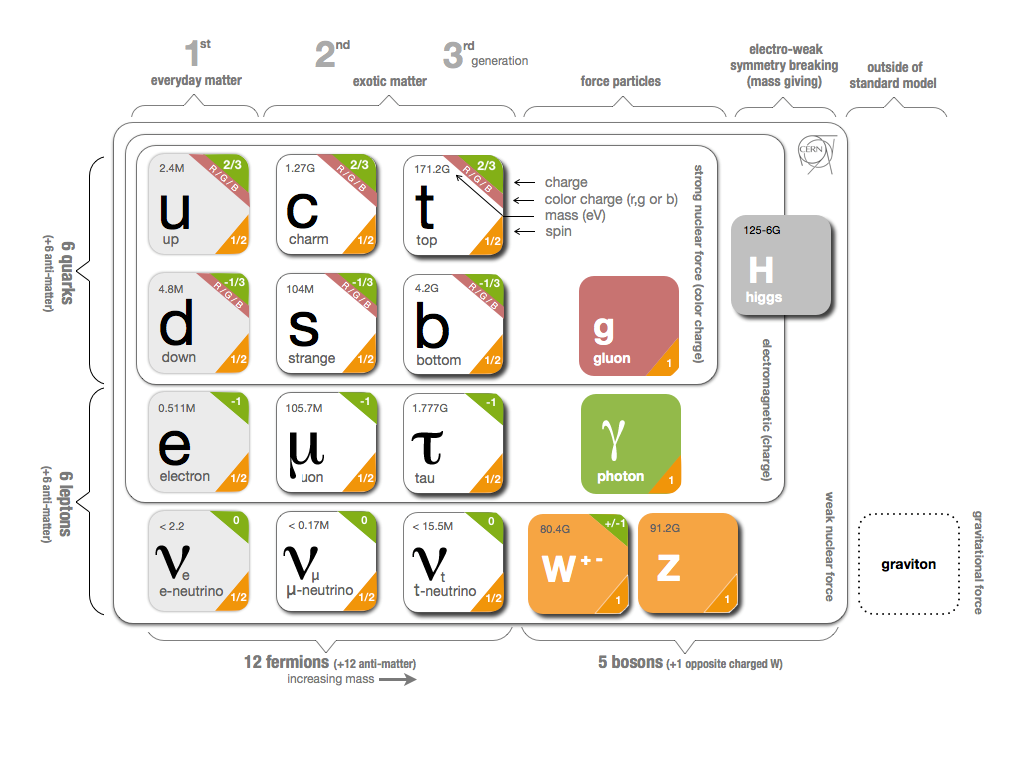
\includegraphics[width=\linewidth]{2_theory/sm}
    \caption{Overview of the particles of the \ac{SM}. All fermions participate in the weak interaction, but only the quarks interact with gluons, whereas both quarks and charged leptons interact with via the \ac{EM} force. Neutrinos, being neutral and colourless, only interact with the \Wboson and \Zboson bosons via the weak force. Finally, the graviton, although it has not been discovered yet, should be the corresponding force carrier of the gravity force. Extracted from \Refn{\cite{SM_diagram}}.}
    \label{fig:theory:sm:particles_interaction:particles}
\end{figure}

Fermions are divided into two kinds of elementary particles: leptons and quarks. There are six leptons classified according to their charge, and are divided into three families or generations, ordered based on their mass. Particles in higher generations have higher mass and are highly unstable, decaying into lower generation leptons. For this reason, matter is built on first generation leptons. The leptons are: electron (\(e\)), muon (\(\mu\)), and tau (\(\tau\)), with their respective neutrinos: electron neutrino (\(\nu_{e}\)), muon neutrino (\(\nu_{\mu}\)), and tau neutrino (\(\nu_{\tau}\)), and properties of each are shown in \Fig{\ref{fig:theory:sm:particles_interaction:particles}}.
There are also six antileptons, which have the opposite charge as the leptons, therefore increasing the number of leptons in the \ac{SM} up to 12. The electron, muon and tau, all have electric charge and sizable mass, while the neutrinos are electrically neutral and have very small mass.

Similarly, there are six flavours of quarks (also having their respective antiparticle): up (\(u\)), down (\(d\)), charm (\(c\)), strange (\(s\)), top (\(t\)), and bottom (\(b\)). Quarks also come in three different colours giving a total of 36 quarks, and only mix in such a way as to form colourless objects. An overview of the quarks and their properties are shown in \Fig{\ref{fig:theory:sm:particles_interaction:particles}}.


Each of the three forces unified in the \ac{SM} is described by a \ac{QFT}, corresponding to the exchange of a boson mediator.
The strong force, mediated by massless gluons, is responsible for binding quarks together. While gluons do not carry electric charge, they possess color charge, which leads to the phenomenon of \textit{color confinement}. Despite being massless, the strong interaction becomes stronger at low energies, confining quarks and gluons within hadrons due to the property asymptotic freedom and the aforementioned property of color confinement.
The \ac{EM} force is mediated between charged particles by photons. Photons do not have mass, and, as a consequence, the interaction has infinite range.
Finally, the weak interaction is mediated by the massive \Wboson and \Zboson bosons, leading to short-range interactions. The fundamental properties of these bosons are also displayed in \Fig{\ref{fig:theory:sm:particles_interaction:particles}}.









\subsection{Mathematical formulation of the \ac{SM}}
\label{subsec:theory:sm:mathematical}

The \ac{SM} is a renormalizable field theory based on local symmetries, providing a description of the fundamental particles and their interactions: the strong, the weak and the \ac{EM}. These interactions span by the requirement that the theory is invariant under local gauge transformations of the symmetry group:
\begin{equation*}
    SU(3)_{C} \times SU(2)_{L} \times U(1)_{Y},
\end{equation*}
where \(Y\) is the hypercharge, \(L\) the left-handed helicity and \(C\) the colour charge, and they represent the conserved quantities of the symmetry group. Every local gauge transformation can be absorbed within a gauge field, with the excitations of the gauge fields called gauge bosons. The \ac{EW} sector of the \ac{SM} \(SU(2)_{L} \times U(1)_{Y} \to U(1)_{\text{EM}}\) describes the weak and \ac{EM} interactions, after the spontaneous symmetry breaking mechanism by virtue of the Higgs potential. The non-abelian group \(SU(3)_C\) with colour charge desribes the strong interactions between quarks and gluons, and the theory is known as \ac{QCD}~\cite{Ellis-1996-book}.

In principle, the particles included in the \ac{SM} are massless, unlike the particles observed in nature. While the equations for the \ac{EW} interactions correctly describe particles like the photon, \Wboson, and \Zboson bosons, they fail to account for their masses. To address this, the concept of \ac{EWSB} was introduced, known as the Brout-Englert-Higgs mechanism~\cite{Higgs-1964_1,Higgs-1964_2,Higgs-1966,Englert_Brout-1964}. This mechanism explains how the \Wboson and \Zboson bosons acquire mass through the spontaneous breaking of the \ac{EW} symmetry, caused by the Higgs scalar field obtaining a non-zero vacuum expectation value. Furthermore, it predicts the existence of a new scalar particle, leading to a new massive boson with spin 0, called the Higgs bosons. This particle was experimentally confirmed in 2012 by the \ac{ATLAS} and \ac{CMS} collaborations at the \ac{LHC}, with a measured mass of \(125.25~\gev\)~\cite{ATLAS-HiggsObservation,CMS-HiggsObservation}.

The \ac{SM} Lagrangian can be separated into two terms: the first one describing the \ac{EW} interaction (\ac{EW} sector) and the second one representing the strong interactions (the strong sector):
\begin{equation*}
    \mathcal{L}_{\text{SM}} = \mathcal{L}_{\text{EW}} + \mathcal{L}_{\text{QCD}}
\end{equation*}








\subsubsection{The \acf{EW} interaction}


\subsubsection{The Higgs mechanism}


\subsubsection{\acf{QCD}}
\label{subsubsec:theory:sm:mathematical:qcd}

The huge effort to describe the rich spectrum of mesons and baryons resonances that were discovered during the 1950s, prompted Gell-Mann and Zweig to propose in 1964 the quark model~\cite{Gellmann-1964,Zweig-1964_1,Zweig-1964_2}, which asserts that hadrons are in fact composites of smaller constituents. Zweig called the elementary particles \textit{aces} while Gell-Mann called them \textit{quarks}, but finally the theory came to be called the quark model.

The quark model was formalised into the theory of \ac{QCD} with quarks carrying an additional quantum number called the colour charge, \(C=R,G,B\). Without colour charge, it would seem that the quarks inside some hadrons exist in symmetric quantum states, in violation of the Pauli exclusion principle.
The theory satisfies the gauge symmetry of the group \(SU(3)_C\), which has eight generators \(T^a = \frac{\lambda_{\alpha\beta}^a}{2}\), with \(\alpha\) and \(\beta\) being the color indices, \(\lambda_{\alpha\beta}^a\) the eight Gell-Man matrices (\(a=1,2,\dots,8\)). These eight generators introduce eight new phyisical gauge fields: the gluons.
Mesons and baryons, hadrons composed of two and three quarks respectively, are \textit{white} singles (neutral color charge) of \(SU(3)_C\). 

The local \(SU(3)_C\) symmetry is obtained by replacing in the lagrangian the covariant derivatives
\begin{equation*}
    D_{\mu} = \partial_{\mu} - i g_s \sum_{a=1}^{8} \frac{\lambda_{\alpha\beta}^a}{2} G_{\mu}^a,
\end{equation*}
where \(g_s\) is the bare \ac{QCD} coupling constant and is usually replaced by \(\alpha_s = g_s^2 / 4\pi\). The Yang-Mills field tensor \(G_{\mu\nu}^a\) for the group \(SU(3)_C\) can be written as
\begin{equation*}
    G_{\mu\nu}^a = \partial_{\mu} G_{\nu}^a - \partial_{\nu} G_{\mu}^a + g_s f_{abc} G_{\mu}^b G_{\nu}^c,
\end{equation*}
where \(f_{abc}\) are the structure constants of \(SU(3)\). It is important to note that the last term in the previous equation describes the gluon auto-interaction, responsible of the non-abelian nature of \ac{QCD}.
The \ac{QCD} Lagrangian density is then given by:
\begin{align*}
    \mathcal{L}_{\text{SM}} \supset \mathcal{L}_{\text{QCD}}
    &=
        -\frac{1}{2} \Tr\left\{G_{\mu\nu}G^{\mu\nu}\right\}
        + 
        \sum_{\text{flavours}} i \bar{q}_f \gamma^{\mu} D_{\mu} q_f\\
    &=
        -\frac{1}{4} \sum_{a=1}^{8} G_{\mu\nu}^a G^{\mu\nu}_a
        + 
        \sum_{\text{flavours}} i \bar{q}_f \gamma^{\mu} D_{\mu} q_f
\end{align*}

\paragraph{Renormalisation}

As mentioned, the \ac{SM} is a renormalisable \ac{QFT}. What this term refers to is briefly detailed in the following. Higher-order effects introduce quantum corrections, e.g., in the calculation of couplings in the \ac{SM}, which must be taken into account. At the same time, the particles in these loops have unbounded momenta, therefore divergences arise in the calculations for both low (\ac{IR}) and high (\ac{UV}) momenta, which must be eliminated for the theory to be consistent with experimental measurements. The process by which divergences disappear or are 'absorbed' by adding a scale dependence to parameters such as couplings or particle masses, is known as renormalisation. In this way the physical lagrangian, with couplings comparable to experiments, can be written as a bare lagrangian, minus a lagrangian containing the divergence-removing terms, at the cost of introducing a scale dependence \(\mu\) of the momentum. Therefore, the renormalisation results in the couplings (and other observables) being non-consistent and varying with \(\mu\). The phenomenom of asymptotic freedom and colour confinement in \ac{QCD} are consequences of this renormalisation process, which is in turn a property of gauge theories.

\paragraph{The running coupling constant \(\alpha_s\)}

One of the consequences of the non-abelian nature of \ac{QCD} appears on the renormalisation of the coupling constant \(\alpha_s\) via the vacuum polarisation diagrams, which ends up depending on the scale \(Q\) of interaction. For \ac{QED}, the vacuum polarisation is induced by virtual \ee pairs, which (shield) the electric charge and result in the coupling decreasing with distance. In contrast, gluons not only produce \qqbar-pairs (which cause an effect similar to \ac{QED}) but also create additional gluon pairs, which tend to anti-screen the apparent colour charge. In the high-energy regime (small distances), the coupling constant can be approximated with a 1-loop calculation in perturbative \ac{QCD}, as follows:
\begin{equation}
    \label{eq:theory:sm:mathematical:qcd:alphas}
    \alpha_s\left(Q^2\right) = 
    \frac{
        \alpha_s\left(Q^2_0\right)
    }{
        1 + \left(11 N_C - 2 N_f\right) \frac{\alpha_s\left(Q_0^2\right)}{12\pi} \log \left(\frac{Q^2}{Q_0^2}\right)
    }
    =
    \frac{
        12\pi
    }{
        \left(33 - 2 N_f\right)  \log \left(\frac{Q^2}{\Lambda_{\text{QCD}}^2}\right)
    },
\end{equation}
where \(N_C\) is the numbers of colors in the theory (3), \(N_f\) is the number of active flavours\footnote{Those quarks with \(m_q \ll Q\), where \(m_q\) is the quark mass after the process of \ac{EWSB} produced by the Higgs boson.}, \(\alpha_s\left(Q_0\right)\) is the value of the coupling constant at a fixed scale \(Q_0\), determined experimentally at the \Zboson mass value squared, and \(\Lambda_{\text{QCD}}\) is the cut-off \ac{IR} scale, where the perturbative approximation in \(\alpha_s\) stops being valid. Experimental measurements, compared to the theory prediction, of the running coupling constant \(\alpha_s\) is shown in \Fig{\ref{fig:theory:sm:mathematical:qcd:alphas}}, showing the excellent agreement between both.

\begin{figure}[ht!]
    \centering
    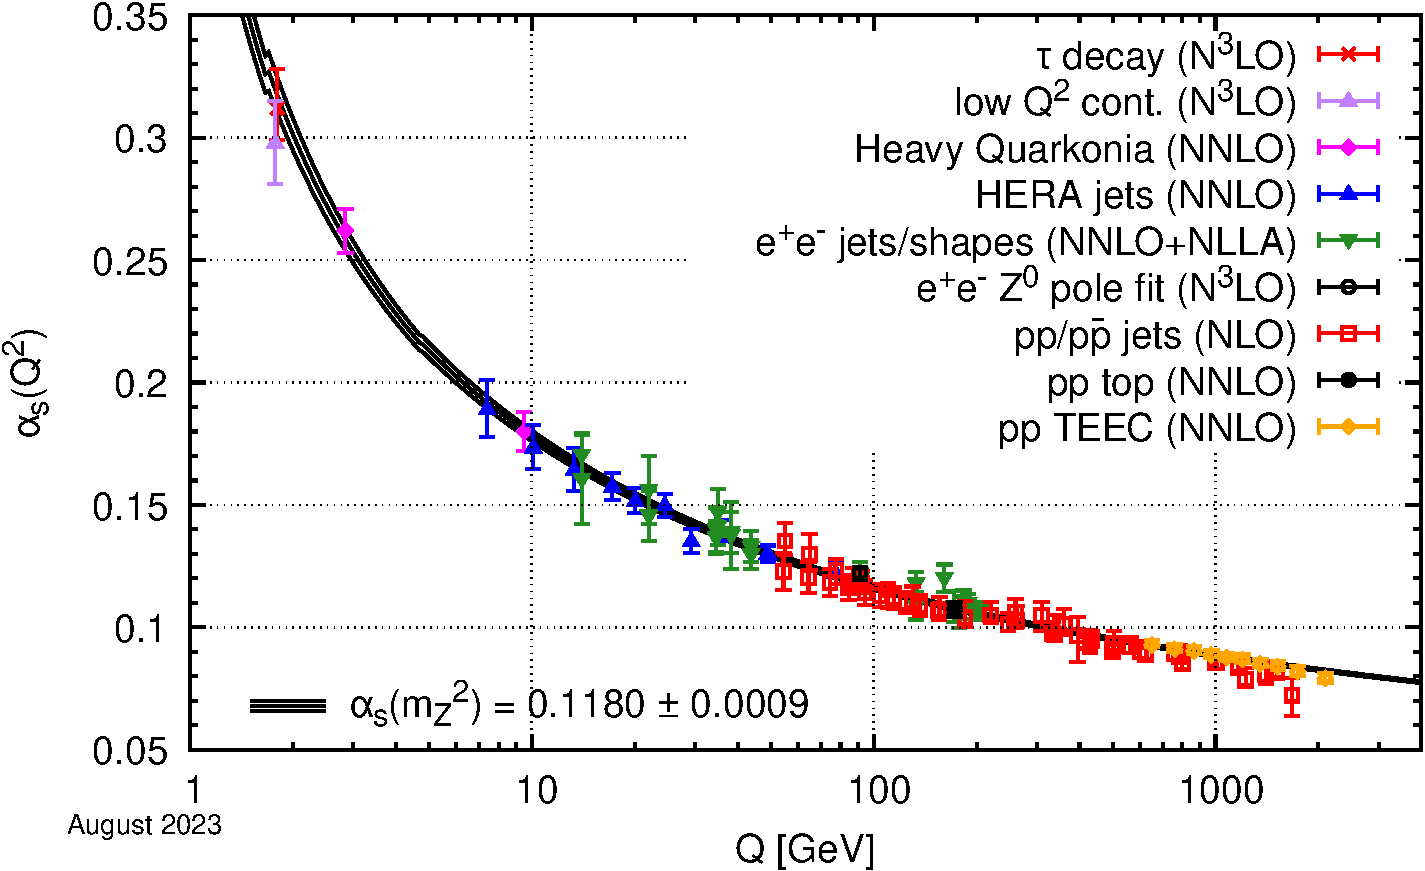
\includegraphics[width=0.6\linewidth]{2_theory/alphas}
    \caption{Experimental measurements of the coupling constant of \ac{QCD} compared to the coupling computed at five loops~\cite{ParticleDataGroup2024}.}
    \label{fig:theory:sm:mathematical:qcd:alphas}
\end{figure}


\paragraph{Asymptotic freedom and confinement}

The coupling constant is said to run, being large at low energy and becoming smaller at high energy. From \Eqn{\ref{eq:theory:sm:mathematical:qcd:alphas}}, at high energies \(\alpha_s \to 0\) therefore \ac{QCD} interacts weakly, allowing the quarks as unbounded particles, phenomenom known as asymptotic freedom~\cite{Wilczek_Gross-1973,Politzer-1973}.
On the other hand, for low energies (\(Q^2 \to 0\)), the coupling \(\alpha_s\) increases divergently, and therefore \ac{QCD} is strongly interacting leading to the confinement of quarks and gluons~\cite{Glashow_Georgi-1974}. Confinement implies that neither quarks nor gluons can appear in isolation, they can only exist within colourless composite "partons", called hadrons.
Moreover, starting from the infrared cut-off scale \(\Lambda_{\text{QCD}}\), where perturbative approximation at \(\alpha_s\) is no longer valid, the creation of quark-antiquark pairs in the vacuum is more energetically favourable than the separation of a pair of bound quarks. For this reason, as they lose energy, the quarks and gluons produced in a proton collider undergo a repetitive process known as hadronisation, in which collimated cascades of hadrons, called jets, are created, forming a cone from the initial quark or gluon to the calorimeters, where all their energy is deposited.


\subsection{Hadron interactions in \pp colliders}
\label{subsec:theory:sm:hadron_interactions}

As discussed in \Sect{\ref{subsubsec:theory:sm:mathematical:qcd}}, the coupling constant \(\alpha_s\), which governs the strong interactions between quarks, has a strong dependence on the energy scale of each interaction, radically modifying the nature of the processes. The modelling of a proton-proton collision in an experiment like \ac{ATLAS}, where it is necessary to know its evolution from the interaction between the protons at \(\sqs \sim \tev\), to the interaction of the particles in the final state with the active and passive materials of the detector at a few GeV, represents a huge challenge, as it covers very different behaving \ac{QCD} regimes. Given that the \ac{LHC} is a proton collider, it is mandatory to have a very precise description of the proton structure, as a \pp collision at very high energies is basically to collide the constituents of them.

At very high energies, but within the perturbative regime, the collision between two protons can be studied via the Parton Model. This model has been introduced by Feynman~\cite{Feynman-1969} and Bjorken~\cite{Bjorken-1969_1} in the late-1960s, to interpret electron-nucleon deep inelastic scattering at SLAC. This description has proven to be a good approximation for parton-parton interactions with large momentum transfer (i.e. Bjorken scaling~\cite{Bjorken-1969_2}) but is not appropriate for modelling the interaction at low energies.
Under this abstraction, the partons include not only the valence quarks (\(u\), \(\bar{u}\) and \(d\) in the case of the proton), but also the pairs of particles and antiparticles in the quark sea, and the gluons that mediate the interactions between them. The model assumes a permanent interaction between partons, so their individual momentum is unknown, although their fraction of momentum with respect to the total hadron momentum can be modelled as a random variable.
Furthermore, in the case of experimental verification, the quarks and gluons in the final state are not directly observed due to hadronisation (concept discussed in \Sect{\ref{subsec:theory:mc_simulation:hadronisation}}). Instead, an effective hadronic cross section, \(\sigma(\pp\to jj)\), is calculated between the incident protons and the final state jets. To perform this passage, the factorisation theorem~\cite{Ellis_Georgi_Politzer_Ross-1978,Feynman-1969,Collins_Soper_Sterman-book,Collins_Soper-1987} is used, which allows a systematic separation between the short-distance interactions (of the partons), and the long-distance interactions (responsible for colour confinement and hadron formation). This theorem states that the total cross-section for two hadrons can be obtained by weighting and combining the cross-sections for two particular partons. This weighting is done using \(f_i(x,Q^2)\), the \acp{PDF1}, which describe the parton density for a parton of species \(i\) in a hadron, with a fraction \(x\) of the hadron energy-momentum when the hadron is probed at a resolution scale \(Q^2\). The cross-section for a hard scattering process \(\pp \to X\), initiated by two hadrons with four-momenta \(P_1\) and \(P_2\) can be written as:
\begin{equation}
    \label{eq:theory:sm:hadron_interactions:xs}
    \sigma_{\pp\to X} = \sum_{ij} \int_0^1 \dd{x_1} \dd{x_2} f_i(x_1, \mu_F^2) f_j(x_2, \mu_F^2) \, \hat{\sigma}_{ij}\left(p_1, p_2, \alpha_s(\mu_R^2), Q^2/\mu_R^2, Q^2/\mu_F^2 \right),
\end{equation}
where \(x_1\) and \(x_2\) are the momentum fractions carried by the interacting partons, and \(p_1 = x_1 P_1\) and \(p_2 = x_2 P_2\) are the interacting parton momenta. The partonic cross-section \(\hat{\sigma}_{ij}\), corresponding to the interaction of partons \(i\) and \(j\), is calculated at a fixed order in \(\alpha_s\), which is evaluated at some renormalisation scale, \(\mu_R\) and factorisation scale \(\mu_F\). The renormalisation scale \(\mu_R\) is important to absorb \ac{UV} divergences in calculations at higher orders. The total cross-section is obtained by summing over all possible parton flavours and integrating over all possible momentum fractions. The parton distribution functions, \(f_i\) and \(f_j\), are evaluated at a factorisation scale, \(\mu_F\) , which can be thought of as the scale that separates short-distance, perturbative physics, from long-distance, non-perturbative physics (i.e., separates hard and soft processes).

If the perturbative expansion were carried to all orders, the cross-section in \Eqn{\ref{eq:theory:sm:hadron_interactions:xs}} would be independent of \(\mu_F\) and \(\mu_R\). However, in actual finite order calculation this does not hold. They are usually both taken to be equal, \(\mu_F = \mu_R = \mu\), chosen at the typical scale \(Q^2\) of the process, in order to minise the contribution of uncalculated higher order terms, whose forms are logarithmic \(\log\left(Q^2/\mu_R^2\right)\) and \(\log\left(Q^2/\mu_F^2\right)\). The dependence of the prediction on \(\mu_R\) and \(\mu_F\) is assigned as a theoretical uncertainty. The fact that the cross-section of a process should be independent of the factorisation scale \(\mu_F\) led to the DGLAP equations (Dokshitzer-Gribov-Lipatov-Altarelli-Parisi)~\cite{Dokshitzer-1977,Gribov_Lipatov-1971,Altarelli_Parisi-1977}. These equations determine the evolution of the \ac{PDF1} with \(Q^2\).
For the case of the proton, \Fig{\ref{fig:theory:sm:hadron_interactions:pdfs}} shows the \acp{PDF1} evaluated at two different factorisation scales for all possible partons.

\begin{figure}[ht!]
    \centering
    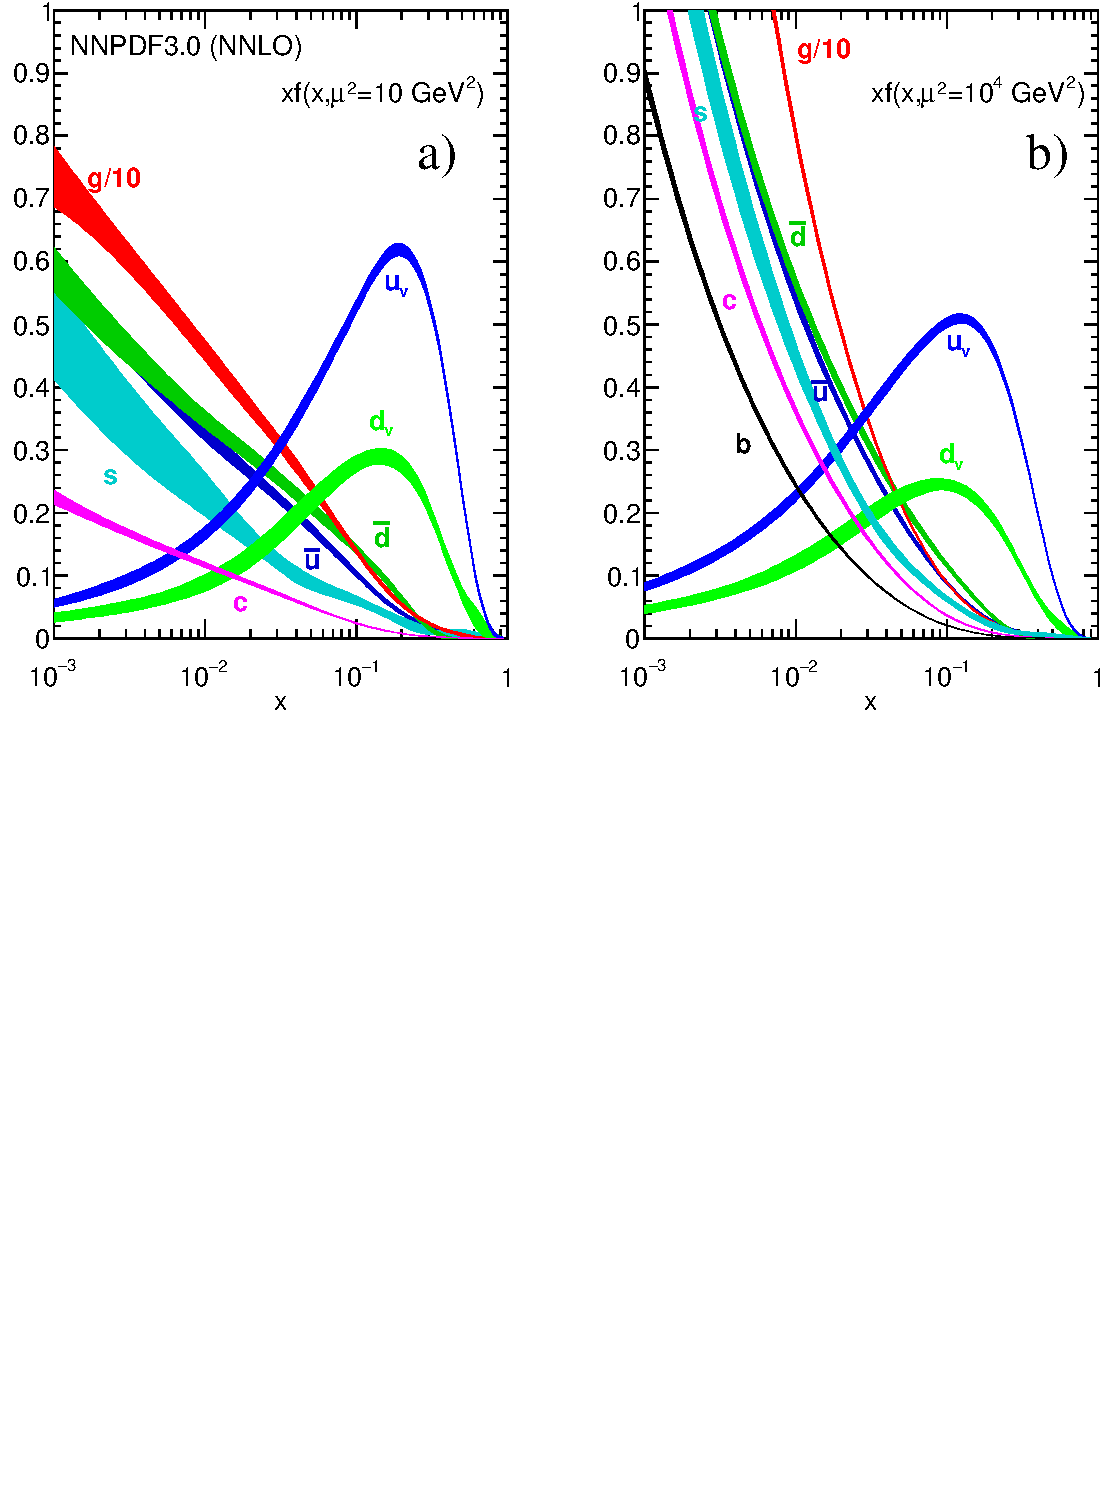
\includegraphics[width=0.7\linewidth]{2_theory/pdfs}
    \caption{Parton momentum fraction \(x\) times the unpolarized parton distributions \(f_i(x, Q^2)\) (where \(i = u_v = u - \bar{u}, \, d_v = d - \bar{d},\, \bar{u},\, \bar{d},\, s\simeq\bar{s},\, c=\bar{c},\, b=\bar{b},\, g \)) obtained in the NNLO NNPDF3.0 global analysis~\cite{NNPDF} at scales \(\mu^2 = 10~\gev^2\) (left) and \(\mu^2 = 10^4~\gev^2\) (right) with \(\alpha_s(M_Z^2) = 0.118\). Figures extracted from \Refn{\cite{ParticleDataGroup2020}}.}
    \label{fig:theory:sm:hadron_interactions:pdfs}
\end{figure}




\subsubsection{Process description}

Initially two hadrons are coming in on a collision course, where each hadron can be thought as a group of essentially collinear partons quantitatively characterised by the parton distributions. In a collision scenario with accelerated particles carrying \ac{EM} and colour charges, bremsstrahlung can occur, e.g. as gluon radiation such as \(q \to qg\). A collision between two partons, one from each side, takes place producing the hard process of interest, that can be calculated by a perturbative approach to some order in \(\alpha_s\), which corresponds to the number of outgoing partons. Emissions that are started off from the two incoming colliding partons are called \ac{ISR}, while radiations from the outgoing partons are referred as \ac{FSR}. With the parton shower development, the colour field strength increases as partons loose energy and they can break up by the production of quark-antiquark pairs. Thus, quarks and antiquarks may combine to produce a primary hadron. The creation of hadrons as a consequence of the confinement phenomenon is referred to as “hadronisation”. The additional products of the collision that are not explicitely related to the hard process (radiation, hadron remnants, products of multiple parton interactions, etc.), are generally grouped altogether and called \ac{UE}. A visualisation of the \pp collision is shown in \Fig{\ref{fig:theory:sm:hadron_interactions:parton_shower}}.



\begin{figure}[ht!]
    \centering
    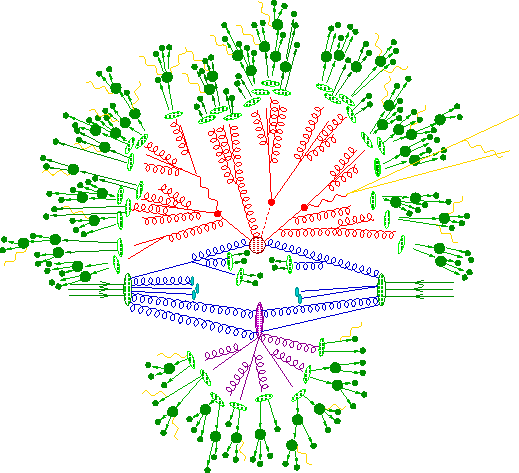
\includegraphics[width=0.7\linewidth]{2_theory/parton_shower}
    \caption{Illustration of the stages of a hadron-hadron collision. The red circle in the center of the figure represents the hard collision, surrounded by a tree-like structure representing bremmstrahlung radiation as simulated by parton showers. The purple blob at the botton represents the \ac{UE}. The hadronisation process is represented by the light green blobs, dark green blobs indicate hadron decays, while yellow lines signal soft photon radiation~\cite{Hoche-2015}.}
    \label{fig:theory:sm:hadron_interactions:parton_shower}
\end{figure}



Over the years, different \ac{LHC} experiments have measured cross sections of different \ac{SM} processes. \Fig{\ref{fig:theory:sm:hadron_interactions:sm_results}} shows the good agreement between the \ac{ATLAS}-measured cross sections of some processes and their theoretical predictions.


\begin{figure}[ht!]
    \centering
    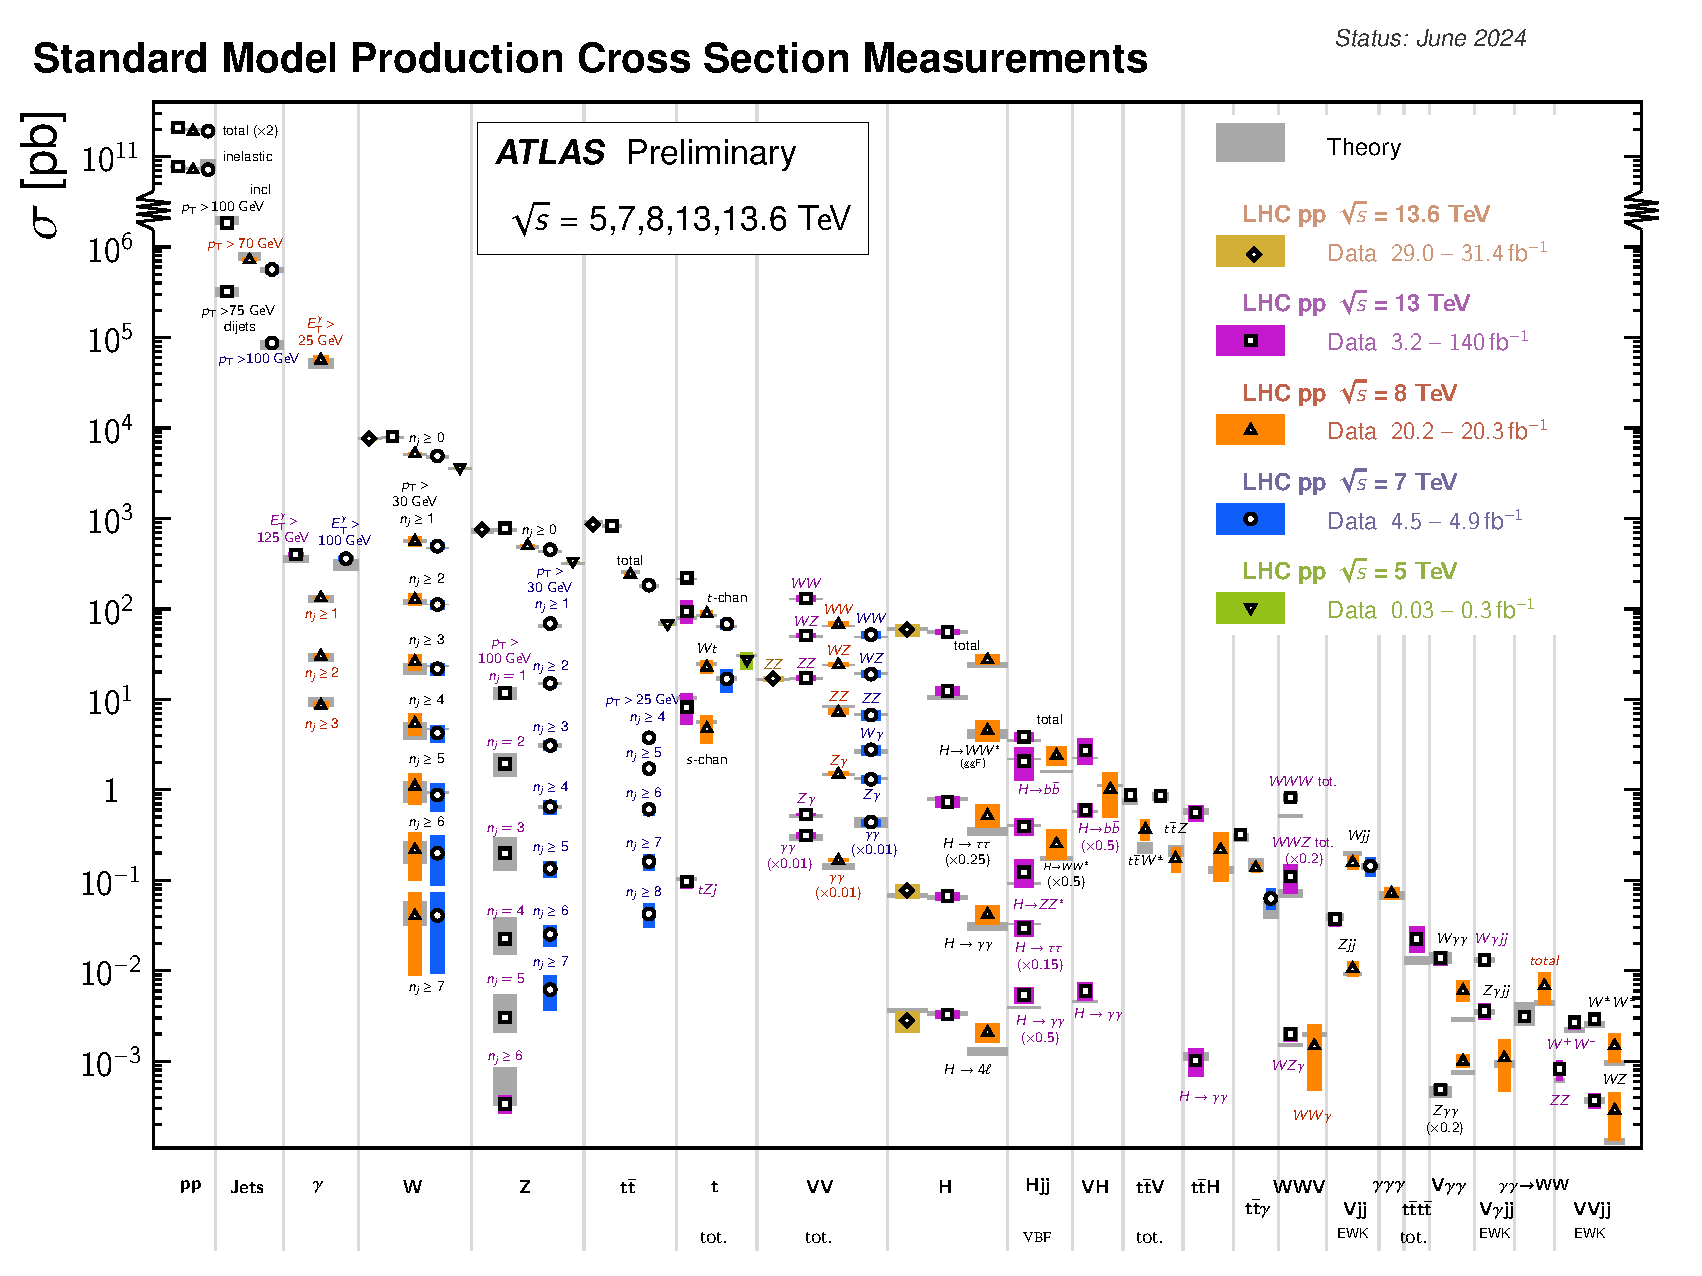
\includegraphics[width=0.8\linewidth]{2_theory/sm_measurements}
    \caption{Summary of several Standard Model total and fiducial production cross-section measurements, compared against their theoretical predictions~\cite{ATLAS-SM_Measurements}.}
    \label{fig:theory:sm:hadron_interactions:sm_results}
\end{figure}



\subsection{Theory of prompt-photon production}
\label{subsec:theory:sm:prompt_photon}


High transverse momentum ("prompt") photons constitute colourless probes of the hard interaction and their  production in proton-proton collisions, \(\pp \to \gamma+X\), provides a testing ground for QCD, whose measurement offers certain advantages over other analyses in jet production events, the most abundant process in single hadron colliders. In this case, the presence of a \ac{QED} vertex at \ac{LO} makes the theoretical calculations more reliable and gives access to a lower range of \pt. Moreover, the energy resolution of electromagnetic calorimeters are in general better than those of the hadronic calorimeter\footnote{A description of both calorimeters is given in \Ch{\ref{ch:atlas}}.}, and systematic uncertainties in the photon energy scale are smaller. Due to the fact that photons do not hadronise (see \Sect{\ref{subsec:theory:mc_simulation:hadronisation}}), the direction and energy of photons is straightforwardly measured in the calorimeter without the need for a jet algorithm to reconstruct a jet.

Prompt-photon production proceeds via two processes: the direct-photon process (D), in which the photon arises directly from the hard interaction, and the fragmentation-photon process (F), in which the photon is emitted in the fragmentation of a high transverse momentum parton~\cite{Szczurek_Pietrycki-2007,Belghobsi_Fontannaz-2009}. From a topological point of view, when a direct photon is produced, it is most likely that it will be separated from the hadronic activity, whereas a photon produced from a fragmentation process, is most probably accompanied by hadrons.

At \ac{LO} in perturbation theory, there are two subprocesses that contribute to the direct-photon production: (a) the Compton process \(qg \to \gamma q\), and (b) the annihilation process \(\qqbar \to \gamma+g\), shown in \Figs{\ref{fig:theory:sm:prompt_photon:feynman_lo_direct:compton}}{\ref{fig:theory:sm:prompt_photon:feynman_lo_direct:annihilation}}. At medium and large \(x\), there is a natural hierarchy of parton distributions in the proton, \(q \gg g \gg \bar{q}\), while at small \(x\), \(g \gg q,\bar{q}\). As a consequence, in proton-proton collisions, the \(qg\) Compton process dominates over essentially all the \pt range. This makes direct photon production particularly useful for constraining the gluon distribution.

\begin{figure}[ht!]
    \centering
    \begin{subfigure}[h]{0.49\linewidth}
        \centering
        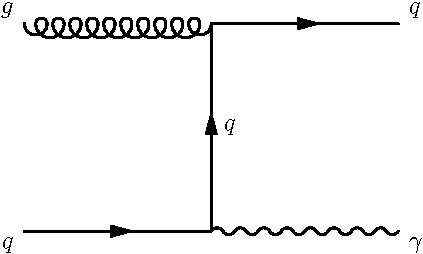
\includegraphics[width=0.7\linewidth]{2_theory/diagrams/gammajet_compton}
        \caption{Compton.}
        \label{fig:theory:sm:prompt_photon:feynman_lo_direct:compton}
    \end{subfigure}
    \hfill
    \begin{subfigure}[h]{0.49\linewidth}
        \centering
        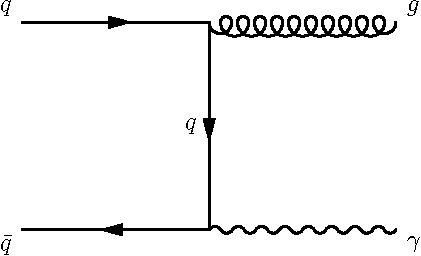
\includegraphics[width=0.7\linewidth]{2_theory/diagrams/gammajet_annihilation}
        \caption{annihilation.}
        \label{fig:theory:sm:prompt_photon:feynman_lo_direct:annihilation}
    \end{subfigure}
    \caption{Feynman diagrams for the \ac{LO} direct-photon production in \pp collisions.}
    \label{fig:theory:sm:prompt_photon:feynman_lo_direct}
\end{figure}

\ac{NLO} corrections to this process are represented in \Fig{\ref{fig:theory:sm:prompt_photon:feynman_nlo_direct}}. In \Fig{\ref{fig:theory:sm:prompt_photon:feynman_nlo_direct:gluon}}, there is a collinear singularity when the momenta of the final-state quark and gluon are parallel. This divergence cancels when real and virtual gluon contributions (see \Fig{\ref{fig:theory:sm:prompt_photon:feynman_nlo_direct:gluon_virtual}}) are summed, and the net effect is a finite \(\mathcal{O}(\alpha_s)\) correction to the \ac{LO} process. On the other hand, in the diagram of \Fig{\ref{fig:theory:sm:prompt_photon:feynman_nlo_direct:photon}} there is another collinear singularity, this time, when the photon and quark momenta are parallel. This singularity, however, does not cancel, but has to be absorbed into a photon fragmentation function \(D_q^{\gamma} (z, \mu^2_f )\) that represents the probability of finding a photon carrying longitudinal momentum fraction \(z\) in a quark jet at scale \(\mu_f\). This fragmentation function is not calculable in perturbation theory, and obeys a DGLAP evolution equation similar to that for the hadron fragmentation functions. The contribution to the cross section from \Fig{\ref{fig:theory:sm:prompt_photon:feynman_nlo_direct:photon}} contains a piece of the form
\begin{equation}
    \label{eq:theory:sm:prompt_photon:fragmentation_contribution}
    \hat{\sigma}(qg \to qg) \oplus D_q^{\gamma} \left(z, \mu_f^2\right).
\end{equation}
The photon-fragmentation contribution appears when a final-state quark-photon collinear singularity occurs in the calculation of the contribution from subprocesses such as \(qg \to gq\gamma\). At higher orders, multiple final-state collinear singularities appear in any subprocess where a high-\pt parton undergoes a cascade of successive collinear splittings ending up with a quark-photon splitting. These singularities are factorised to all orders in \(\alpha_s\) according to the factorisation theorem, and are absorbed into quark and gluon fragmentation functions of the photon, \(D_q^{\gamma} \left(z, \mu_f^2\right)\) and \(D_g^{\gamma} \left(z, \mu_f^2\right)\), respectively.

\begin{figure}[ht!]
    \centering
    \begin{subfigure}[h]{0.32\linewidth}
        \centering
        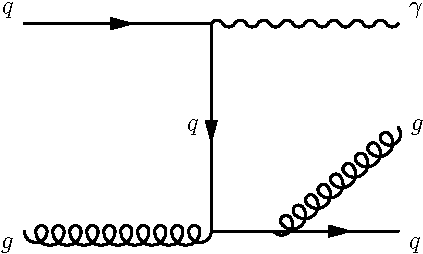
\includegraphics[width=\linewidth]{2_theory/diagrams/gammajet_fsr_gluon}
        \caption{Gluon \ac{FSR}.}
        \label{fig:theory:sm:prompt_photon:feynman_nlo_direct:gluon}
    \end{subfigure}
    \hfill
    \begin{subfigure}[h]{0.32\linewidth}
        \centering
        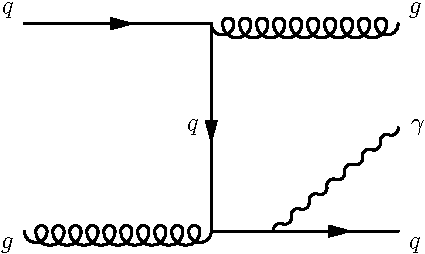
\includegraphics[width=\linewidth]{2_theory/diagrams/gammajet_fsr}
        \caption{Photon \ac{FSR}.}
        \label{fig:theory:sm:prompt_photon:feynman_nlo_direct:photon}
    \end{subfigure}
    \hfill
    \begin{subfigure}[h]{0.32\linewidth}
        \centering
        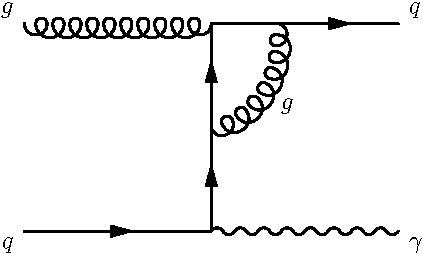
\includegraphics[width=\linewidth]{2_theory/diagrams/gammajet_nlo_direct_virtualcorrection}
        \caption{Virtual gluon correction.}
        \label{fig:theory:sm:prompt_photon:feynman_nlo_direct:gluon_virtual}
    \end{subfigure}\\
    \caption{Feynman diagrams for direct-photon production at \ac{NLO} in \pp collisions.}
    \label{fig:theory:sm:prompt_photon:feynman_nlo_direct}
\end{figure}


The photon fragmentation function increases uniformly with the scale over the whole \(z\) range, i.e. \(D_k^{\gamma} \left(z, \mu_f^2\right) \sim d^{\gamma}(z)\ln(\mu^2)\) as \(\mu^2 \to \infty\). When the \pt is large with respect to \(\sim 1~\GeV\), the \(\ln \pt^2\) growth of the fragmentation function in \Eqn{\ref{eq:theory:sm:prompt_photon:fragmentation_contribution}} compensates one of the \(\alpha_s \left(\pt^2\right)\) couplings in the subprocess cross section, and the contribution is effectively of order \(\alpha_s \left(\pt^2\right) \alpha_{EM}\), i.e. the same as the \ac{LO} contribution. Feynman diagrams corresponding to the \ac{LO} fragmentation component are shown in \Fig{\ref{fig:theory:sm:prompt_photon:feynman_lo_frag}}.



\begin{figure}[ht!]
    \centering
    \begin{subfigure}[h]{0.49\linewidth}
        \centering
        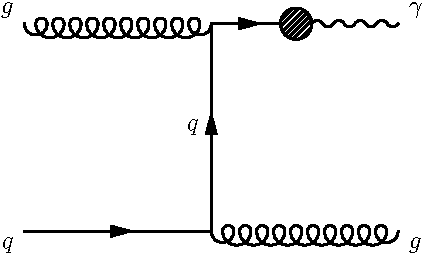
\includegraphics[width=0.7\linewidth]{2_theory/diagrams/gammajet_fragmentation_quark}
        \caption{\ac{NLO} quark fragmentation.}
        \label{fig:theory:sm:prompt_photon:feynman_lo_frag:quark}
    \end{subfigure}
    \hfill
    \begin{subfigure}[h]{0.49\linewidth}
        \centering
        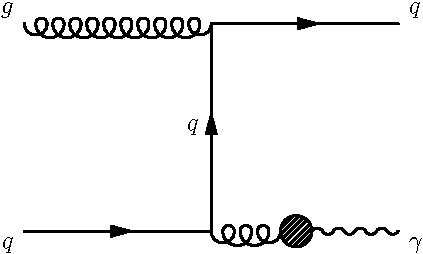
\includegraphics[width=0.7\linewidth]{2_theory/diagrams/gammajet_fragmentation_gluon}
        \caption{\ac{NLO} gluon fragmentation.}
        \label{fig:theory:sm:prompt_photon:feynman_lo_frag:gluon}
    \end{subfigure}\\
    \caption{Feynman diagrams for the \ac{LO} fragmentation-photon processes in \pp collisions (\subref{fig:theory:sm:prompt_photon:feynman_lo_frag:quark}) \(qg \to g q(\gamma)\) and (\subref{fig:theory:sm:prompt_photon:feynman_lo_frag:gluon}) \(qg \to q g(\gamma)\).}
    \label{fig:theory:sm:prompt_photon:feynman_lo_frag}
\end{figure}


The inclusive differential cross section in \(\etgam\) for the production of a non-isolated photon is given by the sum of the direct and fragmentation contributions

\begin{align}
    \dv{\sigma}{\etgam} &= \dv{\sigma_{\text{dir}}}{\etgam} + \dv{\sigma_{\text{frag}}}{\etgam} \nonumber\\
    &= \sum_{a,b=q,\bar{q},g} \int \dd{x_a} \dd{x_b} f_a\left(x_a, \mu_F^2\right) f_b\left(x_b, \mu_F^2\right) \times \nonumber\\
    &\quad
    \left[
        \dd{\hat{\sigma}^{\gamma}_{ab} \left(p^{\gamma}; x_a, x_b, \mu_R, \mu_F, \mu_f\right)}
        +
        \sum_{c=q,\bar{q}, g} \int_{z_{\min}}^{1} \frac{\dd{z}}{z^2} \dd{\hat{\sigma}^c_{ab} \left(p^{\gamma}; x_a, x_b, z, \mu_R, \mu_F, \mu_f\right)} D_c^{\gamma} \left(z, \mu_f^2\right)
    \right]
\end{align}


where \(D_c^{\gamma} \left(z,\mu_f^2\right)\) is the fragmentation function of a parton \(c\) to a photon carrying momentum fraction \(z\), \(f_a \left(x_a, \mu^2_F \right)\) is the \ac{PDF1} of a parton \(a\), \(\mu_R\) and \(\mu_F\) are the standard renormalisation and factorisation scales, and \(\mu_f\) is the fragmentation scale. Corrections to the direct component of the partonic cross section \(\hat{\sigma}^{\gamma}_{ab}\) are known up to the \ac{NNLO} in \ac{pQCD}, while the fragmentation component \(\hat{\sigma}^c_{ab}\) is only known at \ac{NLO}.

At \ac{LO}, the theory calculations for the direct and fragmentation processes converge separately, and can be considered independently. However, this distinction has no physical meaning beyond the \ac{LO}, since both kinds of processes need to be considered at the same time to cancel the final-state infrared and collinear singularities. Therefore, beyond the \ac{LO}, both direct and fragmentation processes cannot be considered separately. From a theoretical point of view, the distinction is defined by an arbitrary choice. It follows from the necessity of factorising the final-state collinear singularities and absorbing them into the fragmentation functions. This factorisation requires the introduction of an arbitrary fragmentation scale \(\mu_f\) , which is a non-physical parameter. More generally, it relies on the arbitrary choice of the factorisation scheme, which defines the finite part of the higher-order corrections that is absorbed in the fragmentation functions together with the singularities; the remaining finite part is then included in the higher-order contributions to the partonic cross sections. The dependence on this arbitrariness, and in particular, on \(\mu_f\), cancels only in the sum of the direct and fragmentation contributions, so only this sum is a physical observable.






\section{Physics \acf{BSM}}
\label{sec:theory:bsm}

The previous section briefly described most of the properties of the \ac{SM}, together with \ac{ATLAS} results showing how well the \ac{SM} agrees with experimental data. Despite being one of the most successful theories in physics in general, the model naturally has a range of validity.
However, it cannot be considered the final theory (the one that could "explain everything"), as it has certain limitations, both from a theoretical and an experiential point of view. The \ac{SM} is still regarded as an effective theory, a low-energy approximation of a more fundamental theory. There are three popular types of new physics theories: (i) models with an extended (family) symmetry or scalar sector, (ii) higher dimensional theory, and (iii) quark-lepton compositeness (namely, the \ac{SM} fermions are not elementary anymore~\cite{Kuhn_Zherwas-1984,Cabibbo_Maiani_Srivastava-1984,DeRújula_Maiani_Petronzio-1984,Baur_Spira_Zerwas-1990,Bhattacharya_Chauhan_Choudhary_Choudhury-2009,Zhan_Li_Liu_Li-2016}).
In the following, a general overview of the main shortcomings of the \ac{SM} are presented. After that, the two last types of new physics theories are discussed, enumerating the theoretical models used in the search carried out in this thesis.

\begin{itemize}
    \item \underline{Gravity:} One of the main limitations of the \ac{SM} is the impossibility of including gravity in the same way as other interactions. Not only is including gravity in the theory not enough to explain the observations, but the mathematics used in the \ac{SM} is practically incompatible with the formulation of General Relativity.
    \item \underline{Hierarchy Problem:} In the context of high energy physics, a hierarchy problem occurs when the fundamental value of some physical parameter (such as a coupling constant or a mass), in some Lagrangian is vastly different from its effective value, which is the value that gets measured in an experiment. Typically the renormalised value of parameters are close to their fundamental values, but in some cases, it appears that there has been a delicate cancellation between the fundamental quantity and the quantum corrections. In general, hierarchy problems are related to fine-tuning of the parameters in the theory. The most well-known case in particle physics is the difference on the \ac{EW} scale \(M_W \sim 10^2~\gev\) and Planck scale, where quantum gravity effects start to take over \(M_P\sim10^{19}~\gev\), whose ratio is \(M_W / M_P \sim 10^{-17}\).
    \item \underline{\acf{DM}:} A hint towards the incompleteness of the \ac{SM} is the presence of \ac{DM}. Based on astrophysical measurements and cosmological considerations~\cite{Zwicky-1937,Rubin_Kent-1970,Planck-2014,Clowe-2006,Brada-2008}, known matter accounts only for \(4\%\) of the total of the universe. On the other hand, \(23\%\) of the total matter is associated with a type of unknown matter, referred as \ac{DM}, since it does not emit \ac{EM} radiation, but is massive as it has considerable gravitational effects on visible matter. The only \ac{SM} particle that could be a viable \ac{DM} candidate is the neutrino, but as its mass is too small to explain these phenomena, it has been discarded.
    \item \underline{Neutrino's masses:} The observation of neutrino oscillation implies that although neutrinos have a very small mass, it is not zero, in contrast to the \ac{SM} prediction. Although there are several mechanisms for including them in the \ac{SM}, there is insufficient evidence to know which is the correct form, and some models propose the existence of new, yet unobserved, heavy particles~\cite{GellMann_Ramond_Slansky-2010,Glashow-1980,Ramond-2005}.
\end{itemize}





\subsection{Quark compositeness theories}
\label{subsec:theory:bsm:qstar}

In quark compositeness theories, the quarks are no longer the fundamental constituents of matter, but rather are bound states of particles often termed \textit{preons}~\cite{Pfeil-1981}. The latter are postulated to experience a hitherto unknown force on account of an asymptotically free but confining gauge interaction~\cite{Hooft-1980}, which becomes very strong at a characteristic scale \(\Lambda\), thereby leading to the aforementioned composites. In many such models~\cite{Pati_Salam_Strathdee-1975,Fritzsch_Mandelbaum-1981,Baur_Fritzsch-1984}, though not all, quarks and leptons share at least some common constituents. Such a hypothesis naturally leads to the existence of excited fermion states at a mass scale comparable to the dynamics of the new binding force.

As the "excited states" do undergo the \ac{SM} gauge interactions, they may be produced at colliders operating at high enough energies. On production, they would decay into \ac{SM} particles, with a particularly favorable channel being the radiative decay into an ordinary fermion and a gauge boson (photon, \Wboson, \Zboson, or gluon). If quarks and leptons are not fundamental constituents but only composites, this fact could, in principle, be revealed either through an accumulation of statistics at energy scales comparable to the compositeness scale \(\Lambda\) at the \ac{LHC}. If \(\Lambda\) is not too high then \ac{EQ}s can be produced on shell, while at energies well below \(\Lambda\), such excitations could manifest themselves through an effective four fermion contact interaction involving \ac{SM} particles alone. 

In general, the interactions between the \acp{EQ} (\qstar) and gauge bosons can be written as~\cite{Zhan_Li_Liu_Li-2016}:
\begin{equation}
    \mathcal{L}_{\text{gauge}} = 
    \frac{1}{2\Lambda}
    \overline{\qstar_R}
    \sigma^{\mu\nu}
    \left[
        g_s f_s \frac{\lambda_a}{2} G_{\mu\nu}^a +
        g f \frac{\tau}{2} W_{\mu\nu} +
        g' f' \frac{Y}{2} B_{\mu\nu} +
    \right]
    q_L
    + \text{H.c},
\end{equation}
where \(G_{\mu\nu}^a\), \(W_{\mu\nu}\) and \(B_{\mu\nu}\) are the field strength tensors of the SU(3), SU(2) and U(1) gauge fields, respectively. The coefficients \(g_s\), \(g = e / \sin \theta\), \(g' = e / \cos \theta\) are the strong and electroweak gauge couplings, \(\lambda_a\) is the Gell-Mann matrix, \(\tau\) is the Pauli matrix, and the weak hypercharge is \(Y = 1/3\), respectively. \(\Lambda\) is compositeness scale and \(f_s, \, f, \, f'\) are parameters determined by composite dynamics, which represent the strength of the interactions between the \acp{EQ} and their \ac{SM} partners. The \(s\) and \(t\)-channel Feynman diagrams for such process are presented in \Fig{\ref{fig:theory:bsm:diagrams}}. Finally, the decay width of \acp{EQ} to a photon and a quark can be calculated at \ac{LO}~\cite{Zhan_Li_Liu_Li-2016}:
\begin{equation}
    \Gamma\left(\qstar \to q \gamma\right) =
    \frac{1}{4}
    \alpha
    \left(f \tau_3 + f' \frac{Y}{2}\right)^2
    \frac{\mq^3}{\Lambda^2}.
\end{equation}
which increases with the \ac{EQ} mass \mq if one considers \(\Lambda = \mq\).


\begin{figure}[ht!]
    \centering
    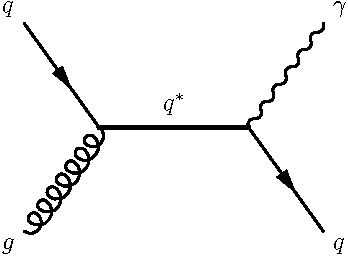
\includegraphics[width=0.3\linewidth]{2_theory/diagrams/qstar_gammajet_s_channel}
    \hspace{1cm}
    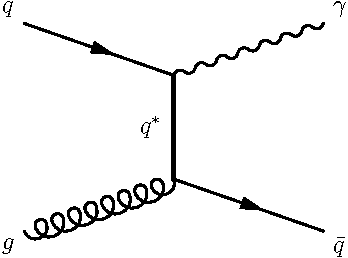
\includegraphics[width=0.3\linewidth]{2_theory/diagrams/qstar_gammajet_t_channel}
    \caption{Feynman diagrams of the \ac{EQ} production in \pp collisions and decay into a quark and a photon in the \(s\)-channel (left) and \(t\)-channel (right).}
    \label{fig:theory:bsm:diagrams}
\end{figure}


In the \ac{SM} there is not a resonance production process decaying into a photon+jet pair in \pp collisions, and direct photon+jet production at tree level occurs via Compton scattering or \qqbar annihilation, as described in \Sect{\ref{subsec:theory:sm:prompt_photon}}. As a result, the \gammajet invariant mass (\myj) distribution is rapidly falling; thus, the \gammajet production mediated by a heavy \ac{EQ} may be discovered if it exists. Hereinafter, in the context of this thesis, \ac{EQ} models are only studied with \gammajet decays. In \fixme{GIVE REFENRECE TO CHAPTER WITH SIGNALS}, information regarding cross sections and the signals signatures in the \ac{ATLAS} detector is given.

\subsection{Higher dimensional theories}

There are at least two seemingly fundamental energy scales in nature, the electroweak scale \(m_{W}~\sim 10^3~\gev\) and the Planck scale \(m_P = G^{-1/2} \sim 10^{18}~\gev\), where \(G\) is the Gravitational constant. Explaining the enormity of the ratio \(m_P / m_W\) has been the prime motivation for constructing extensions of the \ac{SM} such as models with technicolor or low-energy supersymmetry. It is remarkable that these rich theoretical structures have been built on the assumption of the existence of two very disparate fundamental energy scales. However, there is an important difference between these scales. While electroweak interactions have been probed at distances approaching \(\sim m_W^{-1}\), gravitational forces have not remotely been probed at distances \(\sim m_P^{-1}\).

Proposals for a spacetime with more than three spatial dimensions date back to the 1920s, mainly through the work of Kaluza and Klein, in an attempt to unify the forces of nature~\cite{Bailin_Love-1987}. Although their initial idea failed, the formalism that they and others developed is still useful nowadays. Around 1980, string theory proposed again to enlarge the number of space dimensions, this time as a requirement for describing a consistent theory of quantum gravity. The extra dimensions were supposed to be compactified at a scale close to the Planck scale, and thus not testable experimentally in the near future.

A different approach was given by Arkani-Hamed, Dimopoulos, and Dvali (ADD)~\cite{ADD-1998}, where they showed that the weakness of gravity could be explained by postulating two or more flat extra dimensions in which only gravity could propagate. The size of these extra dimensions should range between roughly a millimeter and \(\sim 1/\tev\), leading to possible observable consequences in current and future experiments. Another approach, by Randall and Sundrum (RS)~\cite{RS1-1999_1,RS1-1999_2}, postulates a five-dimensional Anti-deSitter (AdS) spacetime with warped geometry, where the compactification is of the scale of \(1/\tev\).


These low-scale gravity models~\cite{Antoniadis_Arkani_Dimopoulos_Dvali-1998,ADD-1998,RS1-1999_1,RS1-1999_2,Dvali-2008,Dvali-2010} allow for the production of small black holes (\acp{QBH}) in particle collisions~\cite{Argyres-1998,Banks-1999,Giddings-2002}.
\acp{QBH}, unlike semiclassical ones, show significant differences as their mass approaches the Planck scale. Semiclassical black holes decay thermally, losing mass at the Hawking temperature with minimal effect on the surrounding spacetime. However, as the black hole's mass decreases and nears the Planck scale, the influence of back-reaction on the spacetime becomes substantial, and the black hole can no longer maintain thermal equilibrium with its radiation. Microcanonical corrections help refine the decay model, but eventually quantum mechanical effects dominate. When the black hole's Compton wavelength surpasses its Schwarzschild radius, quantum behavior begins to emerge, potentially giving the black hole particle-like properties. At this point, the concepts of a well-defined temperature and entropy break down, making it unlikely that these black holes will decay thermally~\cite{Meade-2008,Alberghi-2006,Alberghi-2007}.

Focusing on black holes with mass slightly above the Planck scale, it's expected that \ac{QBH} decays will not follow a thermal pattern. Instead, decays into only a few particles will likely dominate, and these processes will take place in a small region of spacetime. The \ac{QBH} might behave like a strongly coupled resonance or a gravitationally bound state. After the black hole decays, the \ac{QCD} hadronization process will take place, given the involvement of color charges.

In \pp collisions, only a fraction of the total center of mass energy \sqs is avaiable in the hard-scattering process. By defining \(sx_ax_b \equiv s \tau \equiv \hat{s}\), where \(x_a\) and \(x_b\) are the fractional energies of the two colliding partons (see \Sect{\ref{subsec:theory:sm:hadron_interactions}}), the full cross section \(\sigma\) reads~\cite{Gingrich_Undseth-2020}:
\begin{equation*}
    \sigma_{\pp \to \text{BH} + X}(s) =
    \sum_{a,b}
        \int_{m^2/s}^{1} \dd{\tau}
            \int_{\tau}^{1}
            \frac{\dd{x}}{x}
            f_a\left(\frac{\tau}{x}\right)
            f_b(x)
            \Theta\left(m - m_{\text{th}}\right)
            \hat{\sigma}_{ab\to \text{BH}} (\hat{s} = m^2),
\end{equation*}
where \(a\) and \(b\) go through all the partons, and \(f_a\) and \(f_b\) are the \acp{PDF1} of them. The Heaviside step function \(\Theta\) marks the minimum mass threshold \(m_{\text{th}}\) at which \acp{QBH} could be produced.
The threshold is typically taken to be the Planck scale \(m_P\) for \acp{QBH}, or a few times \(m_P\) for classical black holes. For \acp{QBH} the overall range in which they are considerd to be produced is \(m_P \leq m \leq 3m_P\)~\cite{Gingrich-2010}.
The parton-level cross section \(\hat{\sigma}\) is most often taken to be the geometrical cross-section \(\sigma \sim \pi r_g^2\) with
\begin{equation*}
    r_g = k(D) \frac{1}{m_P} \left(\frac{m}{m_P}\right)^{\frac{1}{D-3}},
\end{equation*}
where \(k(D)\) is a numerical coefficient depending only on the number of dimensions and the definition of the fundamental Planck scale:
\begin{equation*}
    k(D) = 
    \left(
        2^{D-4}
        \left(\sqrt{\pi}\right)^{D-7}
        \frac{\Gamma \left(\frac{D-1}{2}\right)}{D-2}
    \right)
    ^{\frac{1}{D-3}}
\end{equation*}

Based on current experimental and phenomenological limits on the Planck scale, it is unlikely that semiclassical black holes will be accessible at energies produced by the \ac{LHC}. However, if the Planck scale is low enough, \acp{QBH} may be produced in abundance at the \ac{LHC}, and these would appear as resonances in the invariant mass of the final state particles. Concerning only the \gammajet final state, there are six non-thermal black hole states:
\begin{alignat*}{2}
    u + g       & \to QBH^{2/3}     && \to u + \gamma\\
    \bar{d} + g & \to QBH^{1/3}     && \to \bar{d} + \gamma\\
    q + \bar{q} & \to QBH^{0}       && \to g + \gamma\\
    q + g       & \to QBH^{0}       && \to g + \gamma\\
    d + g       & \to QBH^{-1/3}    && \to d + \gamma\\
    \bar{u} + g & \to QBH^{-2/3}    && \to \bar{u} + \gamma,
\end{alignat*}
where \(u\) represents all up-type quarks, \(d\) all down-type quarks and \(q\) all quark flavours. Similarly as the \ac{EQ} model, a more detailed phenomenological description of the models is given in \fixme{GIVE REFENRECE TO CHAPTER WITH SIGNALS}.












\section{\acf{MC} simulations}
\label{sec:theory:mc_simulation}


The \ac{MC} technique is a way of calculating difficult integrals that may be hard to solve by ordinary numerical interpolation methods. High-energy collisions between elementary particles normally produce complex final states, which are populated by many hadrons, leptons, photons and neutrinos. The relation between the final states and the underlying physics description is not simple due to the lack of understanding of the physics and the fact that any analytical approach is not feasible due to the large particle multiplicities. An additional difficulty is related to the need to simulate complicated geometrical factors that represent detectors, a routine situation for experimenters.
\ac{MC} methods allow the generation of complete events with final particles (i.e. hadrons, leptons and photons) together with their momenta, with the same average behaviour and the same fluctuations as the data. Whereas in the data the fluctuations arise from the quantum mechanical character of the underlying theory, in generators these fluctuations are the result of the (quasi-)randomness of the \ac{MC} approach.

The main aspects of the simulated events are: Hard process, Parton Shower, Hadronisation and \acp{UE}, and it follows the schematic representation shown in \Fig{\ref{fig:theory:sm:hadron_interactions:parton_shower}}
The main \ac{MC} event generators used in this thesis are \PYTHIA 8.1~\cite{Pythia8.1}, \PYTHIA 8.2~\cite{Pythia8.2}, \PYTHIA 8.3~\cite{Pythia8.3} and \SHERPA 2.2.2~\cite{Sherpa2.2}.

\subsection{Hard interactions and parton shower}

In order to describe a \(2 \to n\) process from the Lagrangian of the theory (where \(n\) represents a given number of partons in the final state), Feynman diagrams are drawn and evaluated using their specific rules in order to compute the \acp{ME1} in powers of \(\alpha_s\). As the number of partons in the final state increases, the number of Feynman diagrams grows factorially, making higher-order calculations challenging. However, complex processes can be simplified by factoring them into core \(2 \to 2\) processes, which are convoluted with parton splitting probabilities to approximate higher-order effects. Simulation programs implementing this approach are for instance \pythia and \Herwig. These use \ac{LO} perturbative calculations of matrix elements of \(2 \to 2\) processes and implement higher-order \ac{QCD} processes approximately via the so-called initial- and final-state \acp{PS}~\cite{Sjostrand-2006,Dobbs-2004} to produce the equivalent of multi-parton final states.

In a hard process with virtuality \(Q^2\), incoming and outgoing partons emit gluons in a pattern where emissions diverge when gluons become collinear with quarks or when their energy vanishes. Gluon branchings (\(g \to gg\)) exhibit similar divergences, while \(g \to \qqbar\) does not. \ac{NLO} \ac{QCD} programs, such as \Sherpa and \POWHEG, must match \acp{PS} to the \ac{ME1} calculation to avoid double-counting emissions. These emissions, ordered by increasing virtuality, continue until they match the hard process's \(Q^2\). \ac{FSR} similarly decreases parton virtuality until a lower cut-off (\(Q^2_0 \equiv \Lambda_{\text{QCD}} \sim 1~\gev\)) is reached, beyond which perturbation theory loses relevance, and hadronization takes over.

\subsection{Hadronisation}
\label{subsec:theory:mc_simulation:hadronisation}

As the evolution reaches \(Q^2_0 = \Lambda_{\text{QCD}} \), the \ac{PS} phase is truncated since the coupling forces become significant and confinement takes place. This phenomenon cannot still be described from first principles, and therefore, it involves some modelling to transform all the outgoing coloured partons into colourless hadrons of a typical 1 GeV mass scale. The dynamics of this evolution is generally absorbed in fragmentation functions that represents the probability of a parton to fragment into a certain hadron of the final state. Many of these primary hadrons are unstable and decay further at various timescales. Those that are sufficiently long-lived have their decays visible in the detector, or they are stable. There are several models of the hadronisation process, that attempt to connect the results of the \ac{PS} and the final particle spectrum observed. These models can be complemented and tuned using experimental observations. The hadronisation is commonly described by either the Lund string fragmentation model~\cite{Anderson-1983} (as implemented in \Pythia), or the cluster fragmentation model~\cite{Webber-1984} (as implemented in \Herwig and \Sherpa). Essentially, the Lund string fragmentation model asummes a linear confinement, where the energy stored in the colour field between quarks and antiquarks is assumed to increase linearly with the separation of colour charges. Thus, it depicts the colour force by means of a linearly rising potential as charges separate. The potential energy stored increases as partons recede, so it may break up by the production of new quark-antiquark pairs that screen the endpoint colours. Then, quarks and antiquarks may combine to produce hadrons. The cluster fragmentation model is based on the colour preconfinement property of the branching processes, which assumes that the separation of the colour charges forming a singlet are inhibited. After the perturbative parton branching process, the remaining gluons are splitted into light \qqbar pairs, and then neighbouring quarks and antiquarks can be combined into colour singlets (colourless “clusters”), with masses distributions peaking at low values and asymptotically independent of the hard subprocess scale.


\subsection{\acf{UE}}

In addition to the hard interaction that is generated by the \ac{MC} simulation, it is also necessary to account for the interactions between the incoming proton remnants. This is usually modelled through multiple extra \(2 \to 2\) scattering, occurring at a scale of a few GeV. The modelling of the \ac{UE} is crucial in order to give an accurate reproduction of the energy flow that accompanies hard scatterings in hadron colliders. The \ac{UE} can include additional hard interactions and soft processes which can not be calculated perturbatively. These are modelled with adjustable parameters which are tuned to experimental data.



\subsection{Tunes}

Due to the non-perturbative, and therefore incalculable, nature of much of the soft physics processes, like the shower approximations, hadronisation and \ac{UE}, \ac{MC} generators inevitably contain a number of free parameters. These different parameters are usually tuned with data from colliders. A specific set of chosen parameters for a \ac{MC} generator is referred to as a “tune”.
In general, the \ac{ATLAS} \Pythia A14 tune~\cite{Pythia-A14Tune} is used throughout this thesis.
The A14 tune is based on the MONASH tune~\cite{MonashTune} of the \Pythia authors which uses \ee collision data for the hadronisation parameters, and minimum bias \pp collision data at \ac{LHC} to constrain parameters sensitive to initial state radiation and the \ac{UE}. The A14 tune uses in addition a large variety of \ac{ATLAS} data sensitive to multiple parton interactions and \ac{ISR}/\ac{FSR}, and includes jets built from tracks and variables sensitive to the internal jet structure.


\subsection{\acs{ATLAS} detector simulation}

To directly compare the data collected with the \ac{ATLAS} detector with the prediction of \ac{SM} and \ac{BSM} events in simulation, the interaction of the produced particles with the detector material has to be simulated.
The \GEANT~\cite{Geant4} software package is used to simulate the interaction of particles produced in \pp collisions with the different parts of the detector (the \ac{ATLAS} detector is described in \Ch{\ref{ch:atlas}}). \GEANT is an extensive particle simulation package that governs all aspects of the propagation of particles through detectors, based on a description of the geometry of the detector components and the magnetic field. The physics processes include, among others, ionisation, Bremsstrahlung, photon conversions, multiple scattering, scintillation, absorption and transition radiation. The last step involves the digitalisation, which simulates the detector outputs in the same format as the actual raw data. Due to the detailed and complicated geometry of \ac{ATLAS} and the diversity and complexity of the physics processes involved, the consumed computing time per event is large (\(\mathcal{O}\)(1 hour)).

The simulation of a large number of interactions necessary to mimick the \ac{ATLAS} reconstruction is computationally extensive. Especially the simulation of shower developments in the calorimeters consumes a large amount of CPU and computing time. For many \ac{BSM} searches, a large number of parameters affecting the predicted particle masses and interactions have to be simulated, therefore, a "fast" parameterised detector simulation has been developed to cope with this high simulation demand.

A so-called AtlFast3 or AF3~\cite{ATLAS-AF3} (built upon AltFast2~\cite{ATLAS-AF2}) setup simulation chain uses \GEANT~\cite{Geant4} simulation for the interactions in the \ac{ID} and \ac{MS} (described in \Ch{\ref{ch:atlas}}), and two parametrised simulations of the \ac{ECAL} and \ac{HCAL} are used: FastCaloSim V2\footnote{The previous version of AtlFast, called AtlFast2 used FastCaloSim~\cite{ATLAS-FastCaloSim} to simulate the pasage of particles through the calorimeters.}, and FastCaloGAN.
Parametric simulations of the calorimeter response simulate the energy of a particle shower as a single step based on an underlying parametrization instead of simulating how every particle propagates and interacts inside the calorimeter volume.

AtlFast3 introduces several key improvements compared to AtlFast2. Specifically, AtlFast3 enhances the handling of calorimeter showers, significantly improving how energy deposits in the detector cells are simulated. These improvements address limitations in AtlFast2, where sub-cluster structures and lateral shower shapes were not fully described. This new generation also integrates enhanced parameterised simulations and a more precise calorimeter model, leading to improved reconstruction of physics objects like jets and missing transverse energy. These changes lead to better agreement between fast simulation and full simulation results.
Moreover, AtlFast3 supports more advanced algorithms for tracking and calorimeter simulation, ensuring that discrepancies seen in AtlFast2 are minimized, such as inaccuracies in shower shapes and fluctuations.




\FloatBarrier
\part{Experimental setup}
\label{part:exp_setup}
\chapter{The ATLAS Experiment}
\label{ch:atlas}

\epigraph{\emph{Something.}}{Someone}

The work in this thesis has been performed using data from the \ac{ATLAS} detector, one of the particle detectors recording collisions of protons accelerated by the \ac{LHC} particle accelerator at \ac{CERN}. 
In the following chapter, an introduction to the \ac{LHC} is given in \Sect{\ref{sec:atlas:LHC}}, followed by a discussion of the \ac{ATLAS} detector in \Sect{\ref{sec:atlas:atlas}}. The discussion is focused on aspects important to the analyses of this thesis.



\fixme{update chapter, see version in spanish}



\section{LHC}
\label{sec:atlas:LHC}

The \ac{LHC} \cite{LHC-TDR,LHC-Machine} is the largest hadron accelerator in the world, located at \ac{CERN}, in the French-Swiss border. It has a longitude of 27 km, located between 50 and 174 meters underground.
The \ac{LHC} is designed to collide protons (and heavy ions) at a center of mass energy of \(14~\tev\). To keep the protons and heavy ions on the accelerator ring, overall 9593 magnets are used. These magnets include superconducting dipole and quadrupole magnets, cooled down to 1.9 K (-271 $^{\circ} C$). The dipole magnets generate a magnetic field of 8.3 T.

\begin{figure}[ht!]
    \centering
    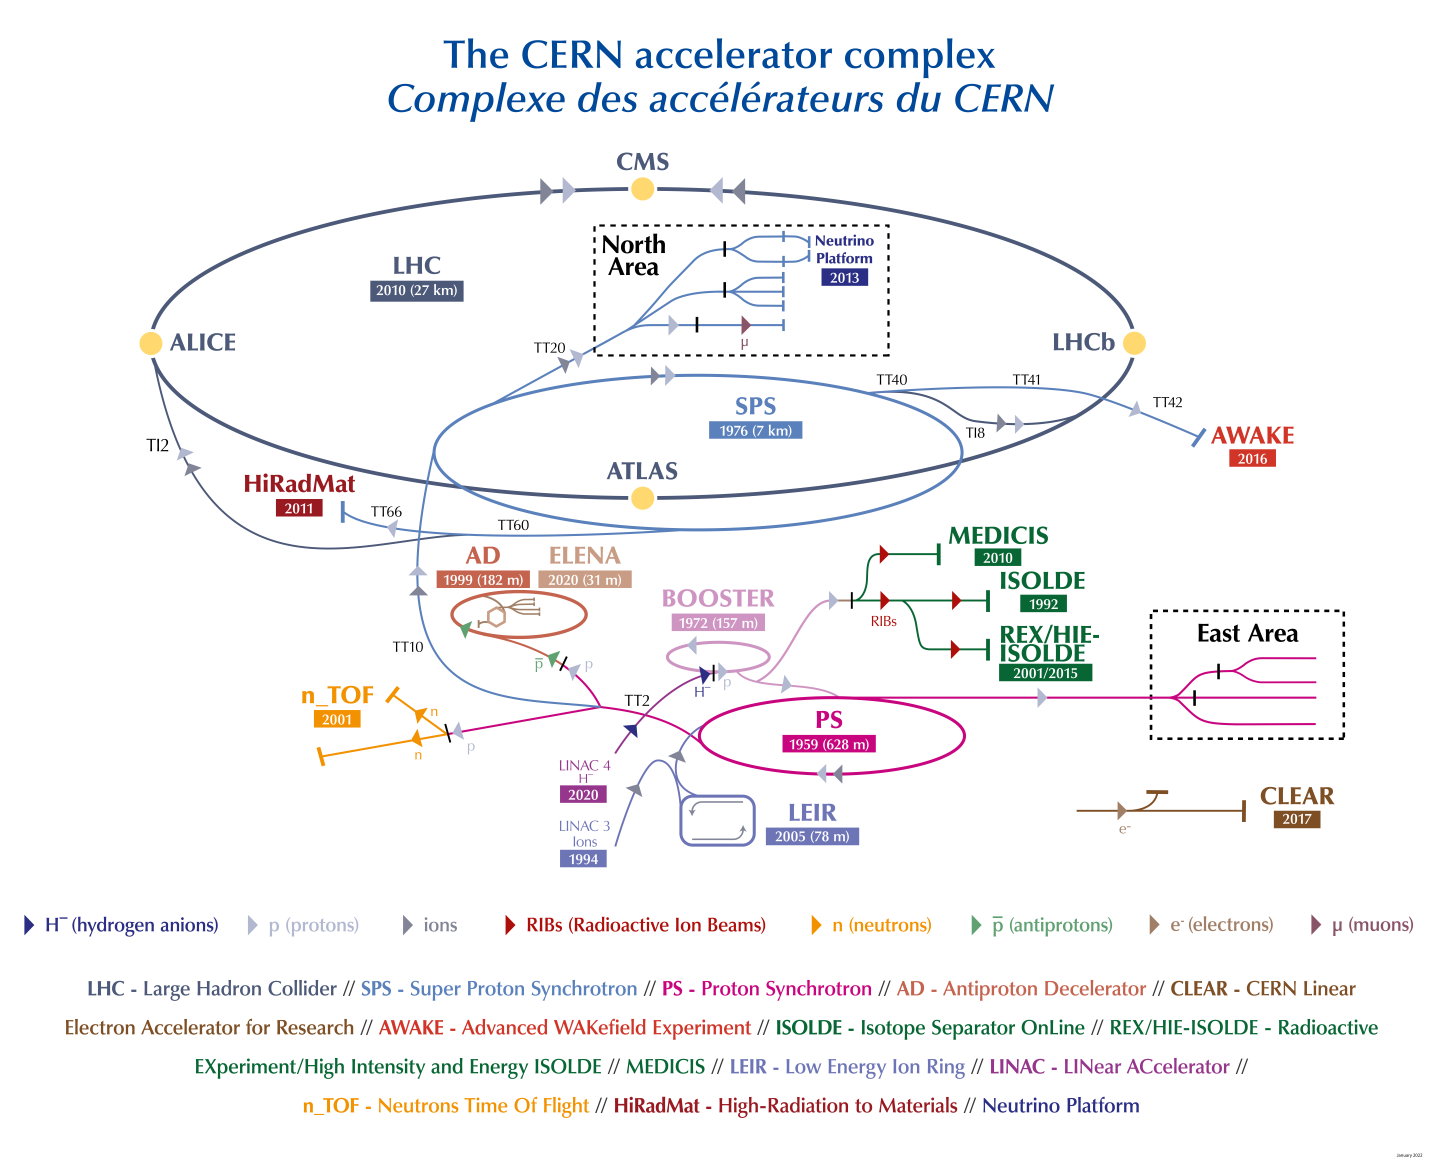
\includegraphics[width=0.75\linewidth]{3_experiment/lhc/AcceleratorComplex2022_large.png}
    \caption{Overview of the \ac{LHC} complex where all the accelerators that lead up to the \ac{LHC} are shown~\cite{LHC-complex}.}
    \label{fig:atlas:lhc:lhc}
\end{figure}

In \Fig{\ref{fig:atlas:lhc:lhc}} a general overview of the \ac{LHC} accelerator facilities is shown. The protons are sourced from hydrogen gas by stripping its electrons and are accelerated in a first linear accelerator (LINAC2) to \(50~\mev\). Subsequently, the protons are successively accelerated in the \ac{PSB}, the \ac{PSync}, and the \ac{SPS}, where they reach an energy of \(450~\gev\) before being injected into the \ac{LHC}.  Overall 8 radiofrequency cavities can push the energy of the protons in the \ac{LHC} up to \(14~\tev\).

The protons are injected as bunches of \(\mathcal{O}(10^{11})\) protons into the \ac{LHC} with a spacing of 25 ns (7.5 m). These bunches are later brought to collision in so-called bunch crossings. The filling scheme of the pre-accelerator chain, in combination with finite switching times of the injection and dumping magnets, results in regular patterns of filled and empty bunches.

The \ac{LHC} so far provided proton and heavy ion beams for two data-taking periods, and is undergoing a third. Between 2009 and 2013 (known as \RunOne), the \ac{LHC} operated with centre-of-mass energy ($\sqrt{s}$) of 7 TeV and 8 TeV.  After a long shutdown (LS1), the second run (\RunTwo) started in 2015 and ended in 2018, providing 13 TeV collisions to the experiments around the \ac{LHC} ring. In 2022 the Run-3 began, at which \pp collisions happen at an energy of \(13.6~\tev\), estimated to run until 2026.
The four yellow dots in shown \Fig{\ref{fig:atlas:lhc:lhc}} there are four interaction points, housing the \acs{ALICE}~\cite{ALICE}, \acs{LHCb}~\cite{LHCb}, \acs{CMS}~\cite{CMS}, \acs{ATLAS}~\cite{ATLAS}, \acs{LHCf}~\cite{LHCf}, \acs{TOTEM}~\cite{TOTEM}, \acsu{MoEDAL}~\cite{MoEDAL} experiments, among many other experiments.


One of the most important parameters to characterize the functioning of the accelerator is the instantaneous luminosity \(\mathcal{L}\), defined as the number of particles per unit time per unit area, and can be calculated from the relation
\begin{equation}
    \mathcal{L} = \frac{N_b^ 2n_b f_{rev}\gamma_r}{4\pi\epsilon_n\beta^*}F
    \label{eq:atlas:LHC:instantaneous_lumi}
\end{equation}
where $N_b$ is the number of particles per bunch, $n_b$ the bunches per beam, $\gamma_r$ is the relativistic gamma factor, $\epsilon_n$ is the normalised transverse beam emittance and $\beta^*$ being the beta function at the collision point which determining the transverse spread of the particle beam. The correction term F takes into account the beam crossing angle. The revolution frequency is represented by $f_{rev}$ which is \(\sim 11~\)kHz, and with the bunch-spacing of \(25~ns\), allows for beam crossing at the four interaction points with a frequency of \(\sim 40~\)MHz. 

A measure for the total recorded data is the integrated luminosity over time is given by
\begin{equation}
    N_{event} = L_{int} \sigma_{event} = \sigma_{event} \int \mathcal{L} dt,
    \label{eq:atlas:LHC:integrated_lumi}
\end{equation}
connecting the luminosity with the number of events. More details regarding the luminosity measurements in \ac{ATLAS} are shown in \Sect{\ref{sec:atlas:runs}}.








\FloatBarrier
\section{ATLAS}
\label{sec:atlas:atlas}

\ac{ATLAS} is one of the multi-purpose detectors of the \ac{LHC}, located at Point-1 along the \ac{LHC}. It was designed and built to study the \pp (and heavy ion) collisions at the \tev scale.

The overall shape of the detector is that of a cillinder as shown in \Fig{\ref{fig:atlas:atlas:atlas}}. It has a length of 44m and 25m in diameter, being the largest particle detector built so far. The \ac{ATLAS} detector is divided geometrically in two parts: the central part called \textit{barrel}, and the outer caps called \textit{end-caps}.

\begin{figure}[ht!]
    \centering
    \includegraphics[width=0.8\linewidth]{3_experiment/atlas/ATLAS_full.png}
    \caption{Overview of the \ac{ATLAS} detector and all its sub-detectors, including the systems added during the \ac{LS2}~\cite{ATLAS-Diagram}.}
    \label{fig:atlas:atlas:atlas}
\end{figure}

\ac{ATLAS} is built in layers of sub-detectors, each of which designed to have a different role on the identification and reconstruction of particles produced in the collisions. \ac{ATLAS} provides hermetic coverage around the beam axis, enabling detection of all charged particles generated in the collisions in the plane orthogonal to the beam axis. This is particularly important in searches for new physics, relying on analyses of momentum balances in the orthogonal plane.

It is built up of multiple layers, starting from the innermost component, the \acf{ID}, providing tracking hits close to the beam pipe. Around the \ac{ID}, there is a superconductor solenoid which creates an axial magnetic field of \(\sim 2\) T to curve the \ac{ID} tracks of charged particles.
After the first magnet, there is a system of two calorimeters: the \ac{ECAL} and \ac{HCAL}. The former is in charge of measuring the kinetic energy of photons and electrons, and the latter measures the energy of the jets.
The outermost parts of \ac{ATLAS} are built by the muon spectrometer, providing momentum reconstruction for muons passing through the inner detector layers. Intertwined with the muon spectrometer, there are a total of 8 barrel toroid coils, providing a total magnetic field of 4 T (0.5 T per coil) to measure the momentum of muons. The toroid magnetic field is completed by the end-cap toroids,  also generating a magnetic field up to 4T for muons leaving \ac{ATLAS} close to the beam pipe.

Every component in \ac{ATLAS} working together enables the reconstruction and identification of a variety of particles with high precision. An overview of the design capabilities of \ac{ATLAS} in terms of the momentum and energy resolution is given in \Tab{\ref{tab:atlas:atlas:expected_performance}}, adapted from \Refn{\cite{ATLAS}}.
Here the resolution given lists first a stochastic term, measuring the uncertainty based on the statistically dominated interaction of a particle with the material, followed by a noise term, which accounts for uncertainties due to electronic noise in the readout process. 


% Please add the following required packages to your document preamble:
% \usepackage{multirow}
\begin{table}[ht!]
    \caption{General performance goals of the \ac{ATLAS} detector. The units of \pt and \(E\) are in \gev. Extracted from \Refn{\cite{ATLAS}}}
    \begin{tabular}{|l|c|c|c|}
        \hline
        \multirow{2}{*}{\textbf{Detector Component}}    & \multirow{2}{*}{\textbf{Required resolution}}     & \multicolumn{2}{c|}{\textbf{$\eta$ coverage}}             \\\cline{3-4} 
                                                        &                                                   & Measurement              & Trigger                        \\ \hline
        Tracking                                        & \( \sigma_{\pt}/\pt = 0.05\%\pt \oplus 1\%    \)  & \( \pm 2.5 \)            &                                \\ \hline
        EM calorimetry                                  & \( \sigma_{E}/E = 10\%/\sqrt{E} \oplus 0.7\%  \)  & \( \pm 3.2 \)            & \( \pm 2.5 \)                  \\ \hline
        Hadronic calorimetry (jets)                     &                                                   &                          &                                \\
        $\quad$barrel and end-cap                       & \( \sigma_{E}/E = 50\%/\sqrt{E} \oplus 3\%    \)  & \( \pm 3.2 \)            & \( \pm 3.2 \)                  \\
        $\quad$forward                                  & \( \sigma_{E}/E = 100\%/\sqrt{E} \oplus 10\%  \)  & \( 3.1 < \abseta< 4.9 \) & \( 3.1 < \abseta< 4.9 \)       \\ \hline
        Muon spectrometer                               & \( \sigma_{\pt}/\pt = 10\%\) at \(\pt =1~\tev \)  & \( \pm 2.7 \)            & \( \pm 2.4 \)                  \\
        \hline
    \end{tabular}
    \label{tab:atlas:atlas:expected_performance}
\end{table}

% \begin{table}[htpb!]
% \includegraphics[width=\linewidth]{figures/ExpSetup/ResolutionATLASDesign.pdf}
% \caption{Performance goals of the \ac{ATLAS} detectors' subsystems.  Units are given in GeV.  $\bigoplus$ indicating a sum in quadrature of the single terms for the total uncertainty \label{tab:expSetup:Resolutions}\cite{ATLAS}. }
% \end{table}


\subsection{ATLAS Coordinate system}
\label{subsec:atlas:coordinates}

\begin{figure}[ht!]
    \centering
    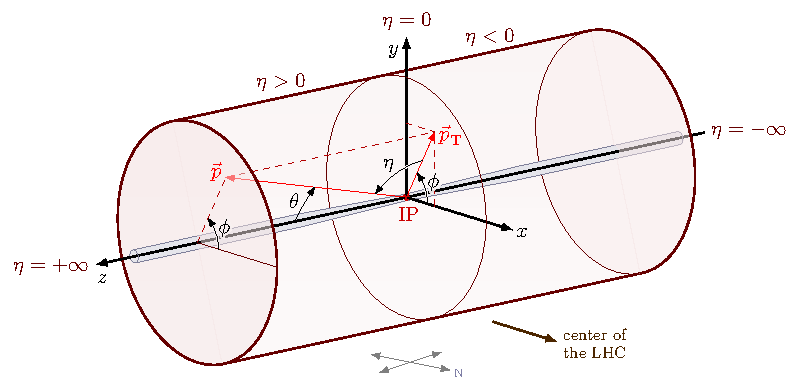
\includegraphics[width=0.8\linewidth]{3_experiment/atlas/ATLAS_coordinates}
    \caption{\ac{ATLAS} coordinate system~\cite{ATLAS-Diagram}.}
    \label{fig:atlas:atlas:atlas_coordinates}
\end{figure}

The coordinate system used within \ac{ATLAS}, displayed in \Fig{\ref{fig:atlas:atlas:atlas_coordinates}}, is used throughout this thesis and shortly described in the following~\cite{ATLAS}. 
The origin of the right-handed coordinate system is at the nominal interaction point, with the positive x-axis pointing towards the centre of the \ac{LHC}.  The x-y plane is perpendicular to the beam axis, defining the z-axis. Towards the surface defines the positive y-axis. An azimuthal angle $\phi$ is defined around the beam axis, and a polar angle $\theta$ is the angle from the beam axis. Instead of $\theta$ the rapidity $y$ is used for heavy objects:
\begin{equation}
    y = \frac{1}{2} \ln[(E+p_z)/(E-p_z)].
\end{equation}
Differences in rapidity are invariant under boosts along the beam axis. For massless objects or relativistic objects ($m << \vb*{p}$),  the pseudorapidity is used instead: 
\begin{equation}
    \eta = -\ln(\tan(\theta/2)).
\end{equation}
To quantify the distance between two objects,  $\Delta R$ is defined:
\begin{equation}
    \Delta R = \sqrt{\Delta\phi^2 + \Delta\eta^2}
\end{equation}
The transverse momentum and energy are defined in the x-y plane, with the transverse momentum given as $\pt = \sqrt{p_x^2 +p_y^2}$.






\subsection{Inner Detector}
\label{subsec:atlas:atlas:id}

\begin{figure}[ht!]
    \centering
    \begin{subfigure}[t]{0.49\linewidth}
        \centering
        \includegraphics[width=\linewidth]{3_experiment/atlas/inner_detector.jpg}
        \caption{\ac{ID} with all its submodules in the barrel and endcap regions~\cite{ATLAS-InnerDetector}.}
        \label{fig:atlas:atlas:atlas_inner_detector:general}
    \end{subfigure}
    \hfill
    \begin{subfigure}[t]{0.49\linewidth}
        \centering
        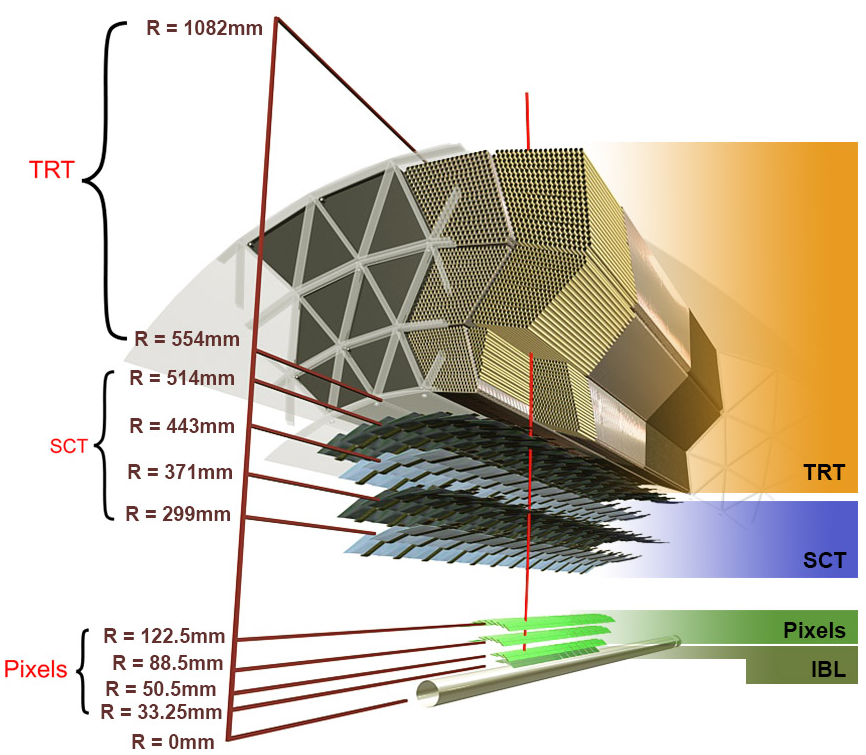
\includegraphics[width=0.8\linewidth]{3_experiment/atlas/inner_detector_layers}
        \caption{Layers of the \ac{ID} showing their distance to the beam~\cite{ATLAS-InnerDetector}.}
        \label{fig:atlas:atlas:atlas_inner_detector:layer_radius}
    \end{subfigure}
    \caption{\ac{ATLAS} \ac{ID} diagrams showing the different submodules, with their corresponding dimensions.}
    \label{fig:atlas:atlas:atlas_inner_detector}
\end{figure}

A cross-section of the \acf{ID} system \cite{ATLAS-ID-TDR} is shown in \Fig{\ref{fig:atlas:atlas:atlas_inner_detector}}, highlighting the distance of each subsystem from the beampipe. The innermost part of the \ac{ID} is the \ac{IBL}, followed by three layers of pixel detectors. At 299 mm radial distance from the beam pipe, four layers of \ac{SCT} modules are located before the \ac{TRT}, which extends the overall \ac{ID} detector size to a radius of 1082 mm. The \ac{ID} allows for particle track reconstruction within $\abseta < 2.5$.


The role of the \ac{ID} is the trajectory tracking of changed particles to determine their charge and momentum. It is immersed in a 2 T magnet field generated by the \ac{ATLAS} solenoid magnet system, that bends the trajectories of charged particles. The curvature radius is proportional to the particle momentum and its direction distinguishes positive from negative charges. The detected particle tracks allow for the reconstruction of primary collision vertices, which is important to distinguish pile-up collisions from the collision of interest, and of secondary decay vertices of longer-lived particles, which is crucial for the identification of e.g. \(B\) mesons or \(\tau\) leptons.


\paragraph{IBL - Insertable B-layer}
After Run-1, during a long shutdown in 2013-2014, the pixel detector system was subject to maintenance and upgrades. Within this set of upgrades, a 4th pixel layer at a 3.3 cm distance from a new, smaller beam pipe (33 mm outer radius, originally 36 mm), whic was the first in particle physics experiments~\cite{ATLAS-IBL-TDR,ATLAS-IBL-proceedings} and has led to significant improvements in interaction vertex reconstruction and identification of b-hadron jets.


\paragraph{Pixel Detector}
The innermost pixel layer, the IBL, is surrounded by three layers of pixel detectors, arranged in barrels around the beam pipe \cite{ATLAS-Pixel-DesignPerformance,ATLAS-Pixel-Performance-Proceedings}. The method of detection of charged particles is the measurement of deposited induced charges in a silicon layer, product of ionization. The first layer is at a distance of 50.5 mm from the beam pipe's centre. As can be seen in \Fig{\ref{fig:atlas:atlas:atlas_inner_detector:general}}, the end caps of the pixel layer consist of 3 disks around the beampipe, stretching the length of the pixel component of the \ac{ID} to 1.4 m length along the beam axis.  The pixel detector consists of overall 1744 pixel modules with a nominal size of $50 \mu m x 400 \mu m$ in the $(\phi, z)$ plane ($\phi, r$ for the disk panels), comprising over 80 million readout channels.  
The pixel and \ac{IBL} part of the \ac{ATLAS} detector is crucial for tracking, providing 4 pixel hits over the entire \ac{ID} pseudorapidity coverage ($|\eta| < 2.5.$).  

\paragraph{Semiconductor Tracker}
The pixel detector and \ac{IBL} are located within \ac{SCT} modules \cite{ATLAS-SCT}.  
Similar to the pixel detector modules, the \ac{SCT} modules are semiconductor-based, arranged into cylindrical layers around the beampipe in the barrel region, forming disks in the endcap. Since the \ac{SCT} modules only provide precise location along one axis, two modules are combined back-to-back and rotated against each other to gain two dimensional spacial information. Four layers are arranged in the barrel, nine disks in each endcap side (see \Fig{\ref{fig:atlas:atlas:atlas_inner_detector:general}}). Including the endcap disks, the \ac{SCT} extends up to $|z| < 2735 mm$.

\paragraph{Transition Radiation Tracker}
The last part of the \ac{ID} is the \ac{TRT} \cite{ATLAS-TRT-DesignPerformance}, in the barrel stretching from 554 mm to 1082 mm radial distance. This detector is composed of 4 mm diameter straw tubes, arranged in parallel to the beam pipe or radially in the barrel and end-cap, respectively. Within $|\eta| < 2.0$, three barrel rings and 18 end-cap units provide typically 36 hits per track. The straws are intertwined with polypropylene fibres for passing through particles to create transition radiation. Inside the straws is a thin tungsten wire, collecting charges drifting through the straws gas mixture (Xe, CO2 and O2). The level of radiation and collected charges in each straw can be used to discriminate between electrons and charged pions.  The \ac{TRT} only offers spatial information in the $(R-\phi)$ plane, no information in the z-direction can be extracted due to the straws orientation. There is a total of 50000 tubes in the barrel region, while the end-caps contain 320000 tubes.








\subsection{Calorimeters}

\begin{figure}[ht!]
    \centering
    \includegraphics[width=0.8\linewidth]{3_experiment/atlas/calorimenters.jpg}
    \caption{\ac{ATLAS} calorimeter system, showing the \acf{ECAL} and the \acf{HCAL}~\cite{ATLAS-Calorimeter-Diagram}.}
    \label{fig:atlas:atlas:atlas_calorimeters}
\end{figure}

As previously mentioned, the \ac{ID} system is surrounded by two calorimeters: the \acf{ECAL} and the \acf{HCAL}, as shown in \Fig{\ref{fig:atlas:atlas:atlas_calorimeters}}. These calorimeters are designed to measure the energy and position of the incident particles, via the deposited energy by the secondary particle cascades produced by the incident ones. It covers the whole \(\phi\) range and up to \(\abseta<4.9\), with a finer granularity in the region that coincides with the \ac{ID}.
The calorimeter system allows for the discrimination between photons and electrons from hadrons (jets). Furthermore, it allows to measure the energetic imbalance (thanks to its total coverage and hermiticity) and it provides the trigger system with the necessary information for the event selection.

Both calorimeters are so-called sampling calorimeters with alternating layers of absorber and active material. The absorber layer triggers a shower development of consecutive interactions with the detector material, the active layer detects the signal.
The shower development and properties are of vital importance for the particle identification, as it will be shown later.
Two important quantities in connection with the calorimeters are the radiation length, $X_0$, and the interaction length $\lambda$. The radiation length refers to the distance after which an particle (electrons for example) energy has been reduced to \(1/e\) of its initial energy. The interaction length describes the mean free path before the occurrence of an hadronic interaction.

The design resolution of the system on the calorimetric energy is given by
\begin{equation}
    \frac{\sigma(E)}{E} = 
    \frac{a}{\sqrt{E}} \oplus b \oplus \frac{c}{E}
\end{equation}
where \(\oplus\) means that the terms are summed in quadrature. The stochastic term \(\frac{a}{\sqrt{E}}\) is related with the fluctuations on the shower developments, the constant term \(b\) takes into account the inhomogeneities of the detector, and the last term is associated with the electronic noise and is proportional to \(\frac{1}{E}\). The value of the coefficients \(a\) and \(b\) depend on the incident objects. For the electrons' case in the \ac{ECAL}, \(a\sim 10\%~\gev^{1/2}\) and \(b~\sim 0.7\%\), while those for charged pions in the center of the detector are \(a~\sim50\%~\gev^{1/2}\) and \(b\sim5\%\) \cite{ATLAS-Calorimeters-PerformanceRun2}.



\subsubsection{Electromagnetic Calorimeter - ECAL}
\label{subsubsec:atlas:atlas:cals:ecal}

The \ac{ECAL} specializes on the detection of electrons, positrons and photons, which deposit their energy in relatively dense showers: energetic electrons that radiate Bremsstrahlung photons, while energetic photons convert to electron-positron pairs when traversing the dense material.
The absorber is made of lead (Pb) with stainless steel sheets, while \ac{LAr} is used as the active material with copper and kapton electrodes for readout.


The calorimeter has an accordion geometry which provides complete \(\phi\) symmetry without azimuthal cracks. 
It is divided into two half barrels covering the central detector region (\(\abseta<1.475\)), with a small (4 mm) gap at $z = 0$ and one end-cap on each side of the beamline (\(1.375<\abseta<3.2\)).
The transition region between the barrel and end-cap is referred as the \textit{crack} region, and the majority of physics analysis using the \ac{ECAL} require that the photons and electrons are outside of it.
Additionally, the \ac{LAr} technology is used for the hadronic calorimeters end-caps as well as a \ac{FCAL} ($3.1 < \eta < 4.9$).

The thickness of the \ac{ECAL} is over 22 radiation lengths (\(X_0\)) in the barrel region, while over \(24 X_0\) in the end-cap region. For photons, the distance at which the energy dropped to \(1/e\) is \(9/7 X_0\), therefore all the photon's electromagnetic energy is deposited in the \ac{ECAL}, and only a small part reaches the \ac{HCAL}.

The mode of measurement is as follows. The incident particles interact with the absorbent medium (Pb), initiating a shower of charged and neutral particles. The charged particles ionize the \ac{LAr} medium and the electrodes, with the help of an applied magnetic field, collect the electrons produced in the ionization process. The total signal of the active medium is then proportional to the total real energy of the incident particle.

\begin{figure}[ht!]
    \centering
    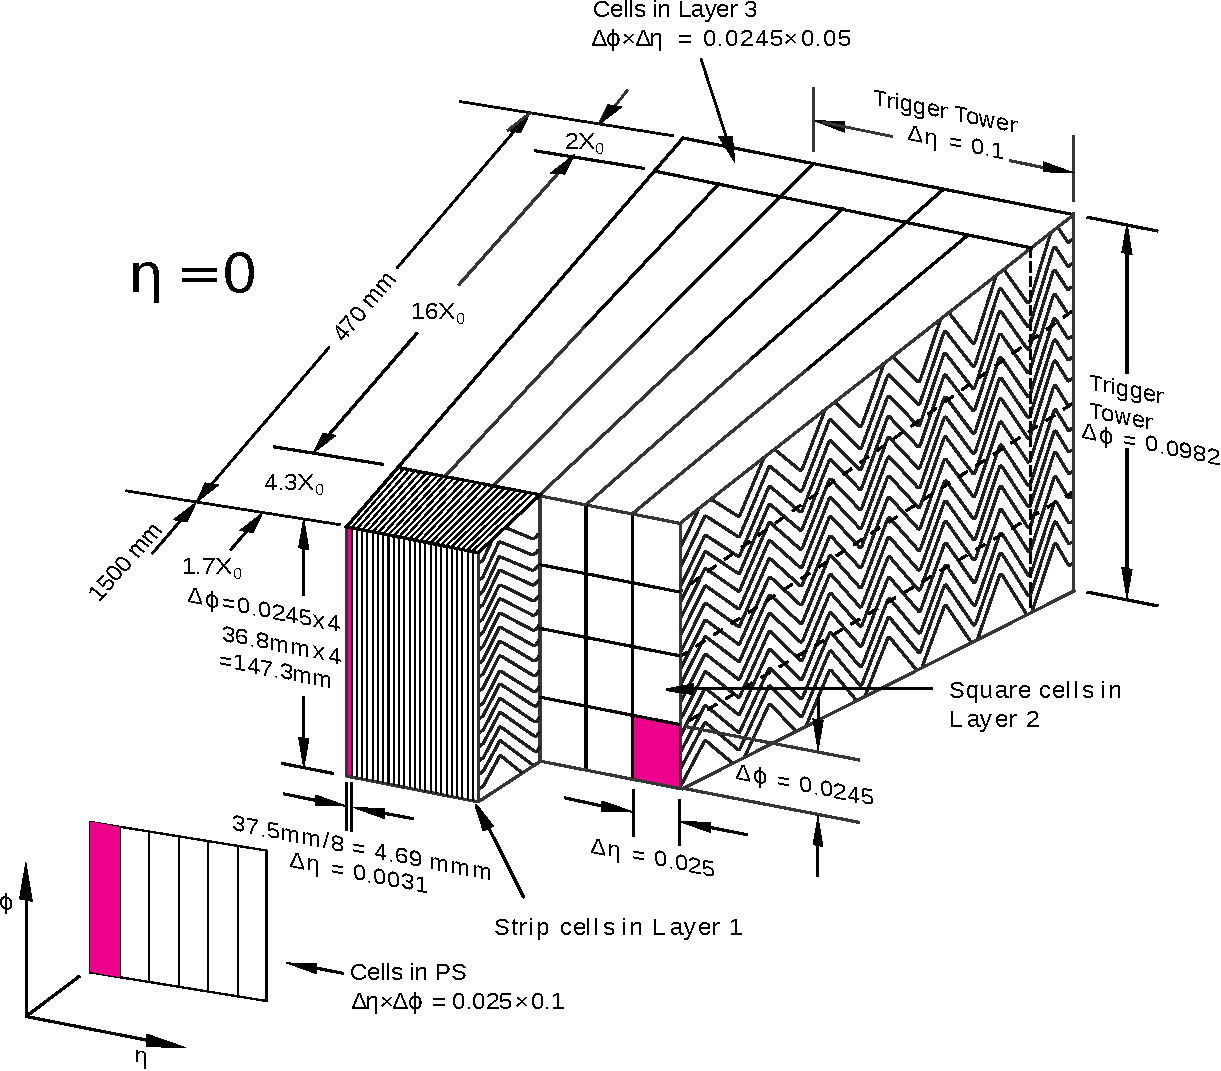
\includegraphics[width=0.8\linewidth]{3_experiment/atlas/ecal_cells}
    \caption{Segment of the \ac{ECAL} showing the layer arrangement and cell dimensions in each layer~\cite{ATLAS}.}
    \label{fig:atlas:atlas:cals:ecal:ecal_cells}
\end{figure}

\begin{figure}[ht!]
    \centering
    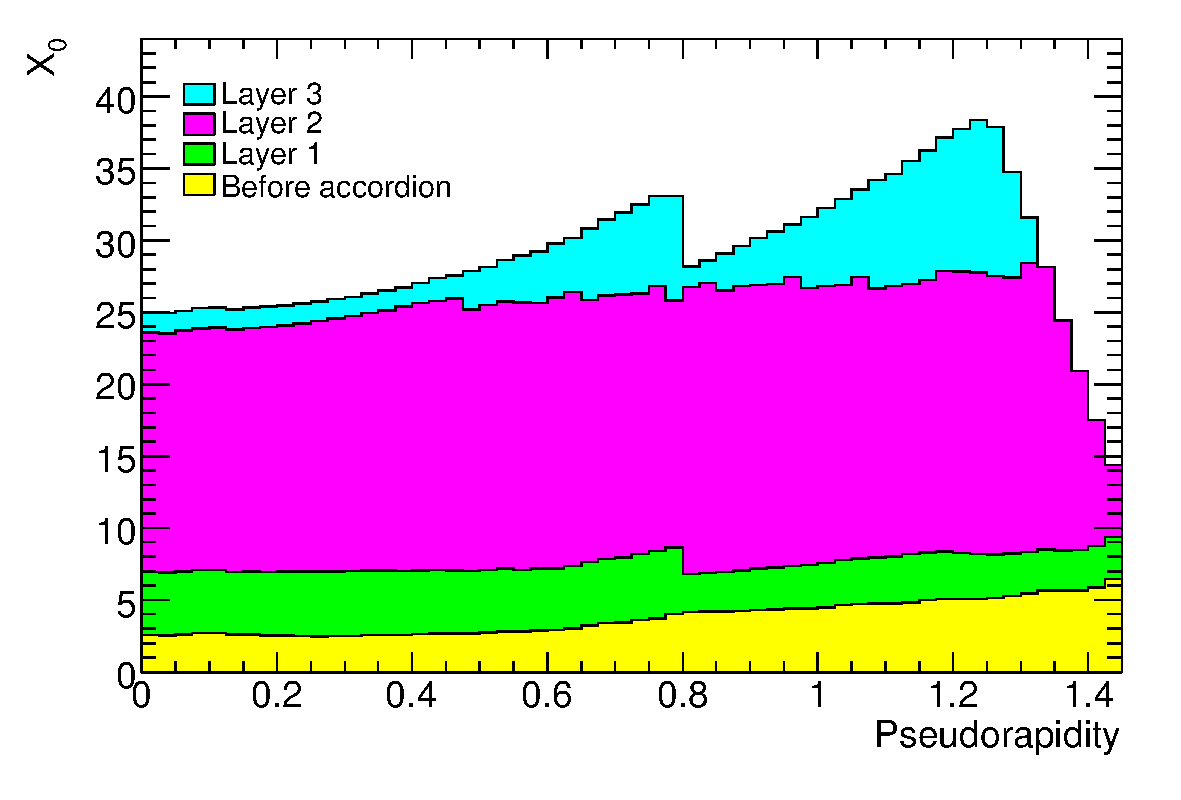
\includegraphics[width=0.46\linewidth]{3_experiment/atlas/ecal_radiation_lengths1}
    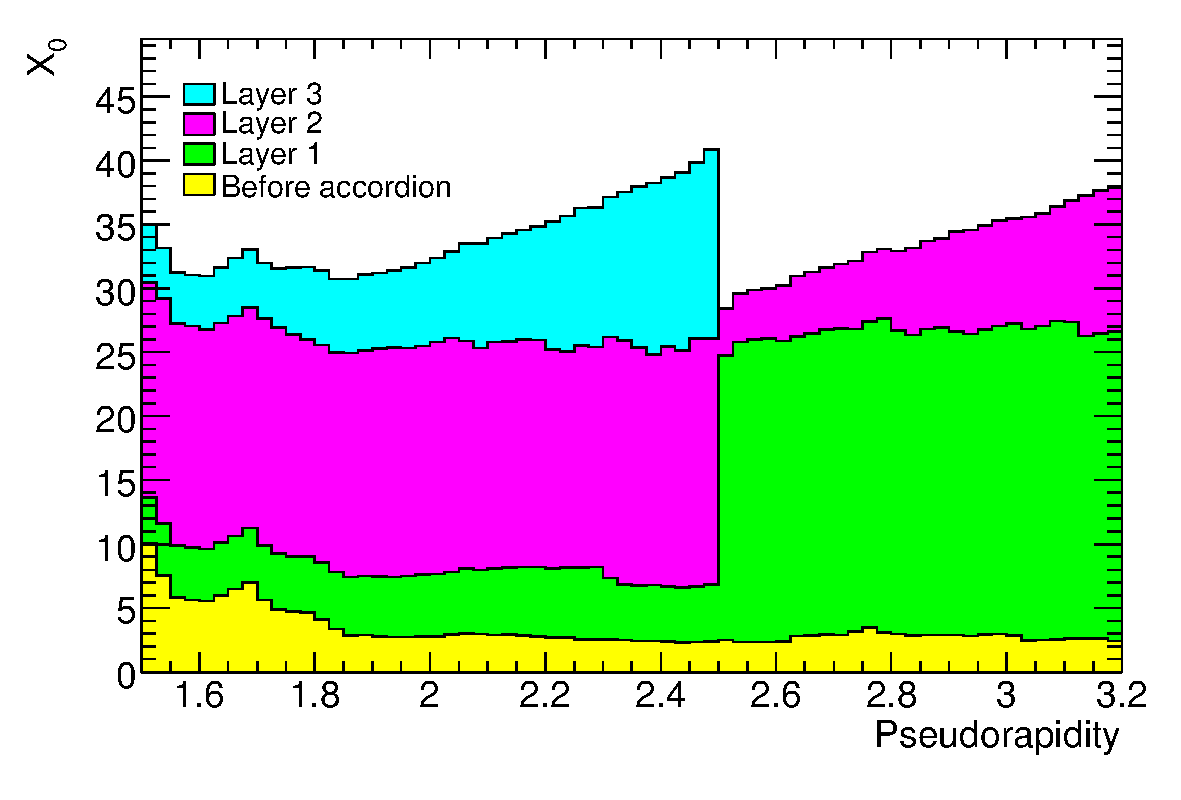
\includegraphics[width=0.46\linewidth]{3_experiment/atlas/ecal_radiation_lengths2}
    \caption{Radiation lengths as a function of \abseta for the \ac{ECAL}, separated for each sublayer~\cite{ATLAS}.}
    \label{fig:atlas:atlas:cals:ecal:ecal_radiation_length}
\end{figure}

Within the region accepted for precision measurements (\(\abseta<2.5\) excluding the crack), the \ac{ECAL} is segmented in three longitudinal layers, displayed in \Fig{\ref{fig:atlas:atlas:cals:ecal:ecal_cells}}.
The first layer consists on fine-granularity bands (also called the strip layer) which helps with the discrimination between isolated photons and pairs of photons spacialy closed originating from \(\pizero\to\gamma\gamma\) decays. This layer has a constant thickness of \(\sim 6 X_0\) as a function of \(\eta\) (see \Fig{\ref{fig:atlas:atlas:cals:ecal:ecal_radiation_length}}), and provides a precise measurement of this variable.
For high energy photons and electrons, the majority of their energy is collected in the second layer, which has a lateral granularity of \(0.025 \times 0.025\) in \((\eta, \phi)\) and a thickness of \(\sim 24 X_0\).
The third layer collects the energy deposited by the tails of the electromagnetic shower, with thickness that varies between 2 and 12 \(X_0\).
There is also a presampler (not shown in figures), that covers the region \(\abseta<1.8\) that improves the energy measurement for particles that start showering before entering the calorimeter.




\subsubsection{Hadronic Calorimeter - HCAL}



Three hadronic calorimeter layers surround the \ac{ECAL} and provide additional discrimination for electrons and photons when measuring the hadronic energy. The \ac{HCAL} extends in pseudorapidity up to \(\abseta<4.9\), allowing virtually the entirety of the solid angle to be covered from the interaction point. In the barrel region (\(\abseta<1.7\)), the tile calorimeter, a sampling calorimeter using steel as absorbing material and plastic scintillator tiles as active material~\cite{ATLAS-Tile-TDR}, is located. It is divided into two parts (\(\abseta<1.0\) and \(0.8<\abseta<1.7\)). The scintillators, arranged in a periodic array, are connected to an optical fiber that carries the light produced by the passing particles to a photomultiplier tube. This array extends, in \(R\), from 2.28 to 4.25 m. In the endcap region (\(1.5<\abseta<3.2\)) there is an hadronic sampling calorimeter, the \ac{HEC}, with copper plates as absorber and liquid argon as active material. Each side of the endcap consists of two wheels, one behind the other with the flat Cu plates arranged perpendicular to the beam axis, with a radius of 2.3 m. Finally there is the \ac{FCAL}, a sampling calorimeter that extends the coverage of the system to \(\abseta<4.9\), coaxial to the beam axis and located 4.7 m on either side of the interaction point. The main material of the modules is \ac{LAr} (with copper or tungsten), and while not used for precision measurements, it provides information for computation of the missing transverse energy and reconstruction of jets in regions very close to the beam axis.

The \ac{HCAL} has a thickness greater than \(7.7~\lambda\) in the barrel region (\(9.7~\lambda\) in total if the \ac{ECAL} is counted). Analogous to the radiation length mentioned for the \ac{ECAL}, a hadronic interaction length is defined as the average distance over which the energy of a hadron is reduced to \(1/e\) of its initial energy. Thus, all the energy with which the hadrons arrive at the \ac{HCAL} is deposited there.





\subsection{Muon spectrometer}

\begin{figure}[ht!]
    \centering
    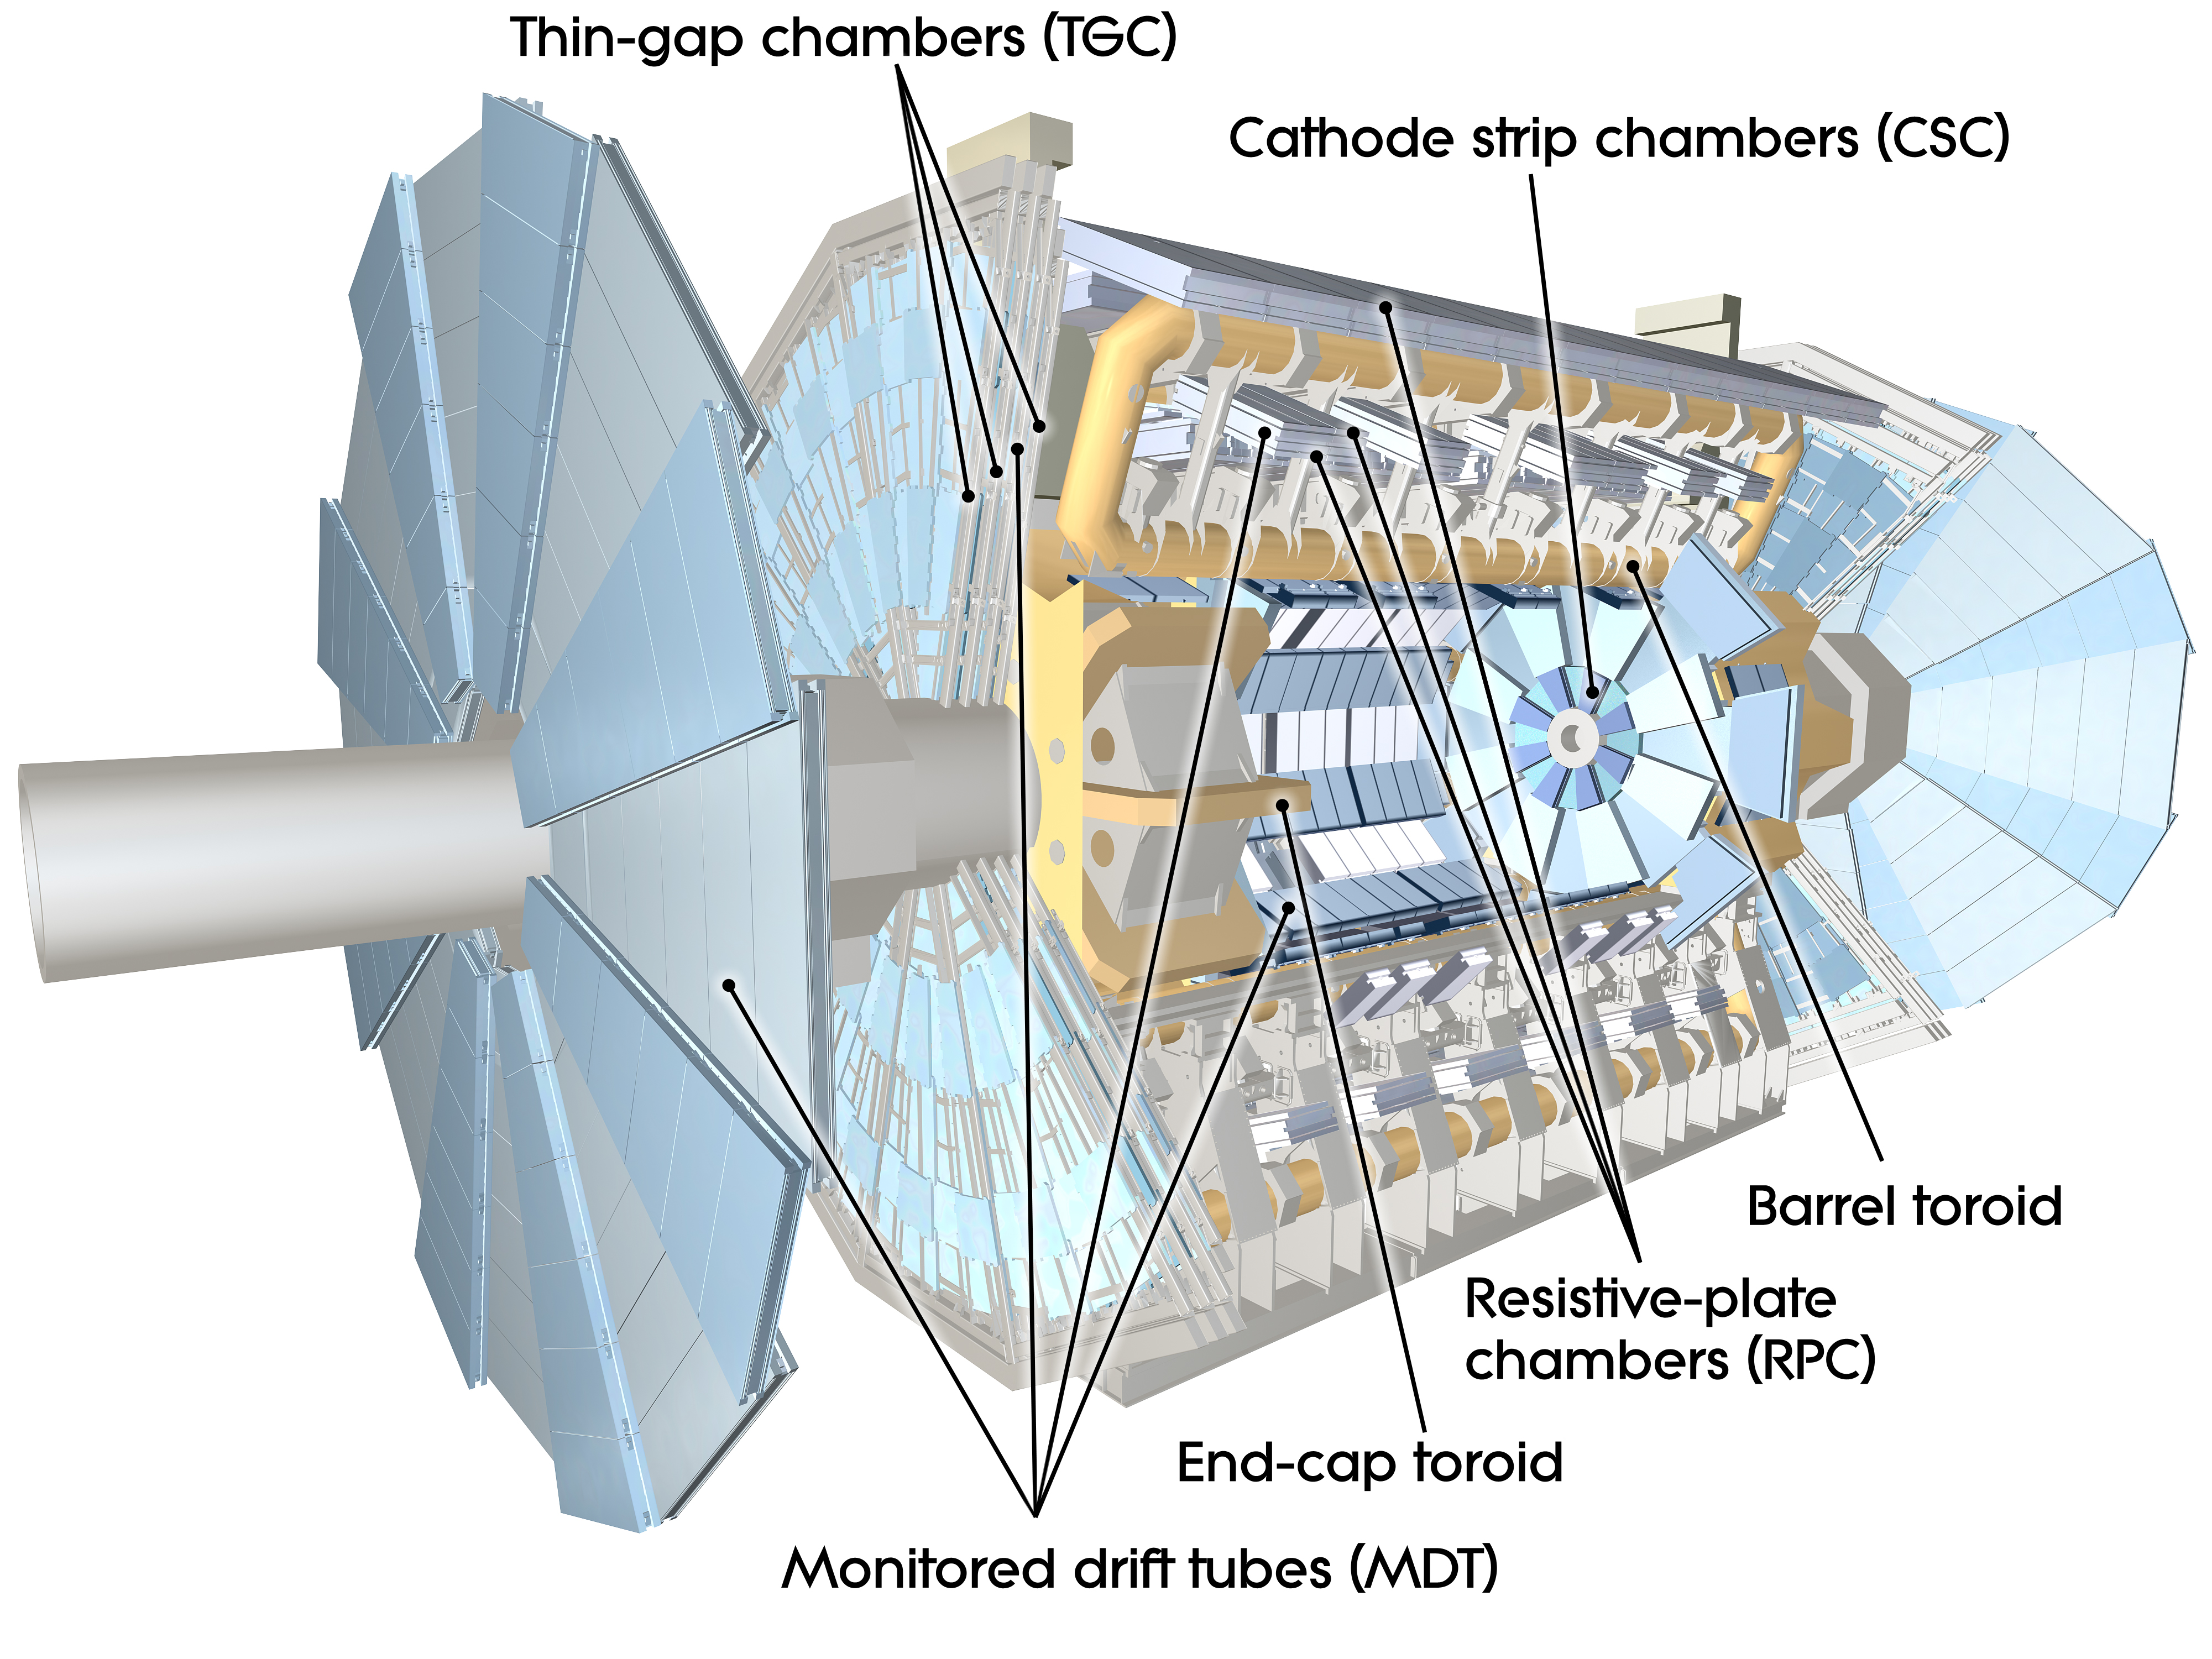
\includegraphics[width=0.7\linewidth]{3_experiment/atlas/muon_detector}
    \caption{\ac{ATLAS} \acf{MS}~\cite{ATLAS}.}
    \label{fig:atlas:atlas:muon_spectrometer:muon_spectrometer}
\end{figure}

The high \pt muons generated at the interaction point have very high penetrating power and are poorly interacting. Therefore, the \ac{MS} \cite{ATLAS-Muon-TDR} is located in the outermost part of the \ac{ATLAS} detector, embedded within the 4 T magnetic field generated by the barrel and endcap toroid magnets, and is designed to obtain high precision position and momentum measurements of high \pt muons. This is the largest subdetector and the one that gives \ac{ATLAS} its size.

The \ac{MS} is designed to precisely measure muons within \(\abseta<2.7\) and to provide muon trigger information up to \(\abseta<2.4\), shown in \Fig{\ref{fig:atlas:atlas:muon_spectrometer:muon_spectrometer}}, highlighting the different subsystems

The \ac{MS} is composed of different types of muon detection chambers (see \Fig{\ref{fig:atlas:atlas:muon_spectrometer:muon_spectrometer}}). \acp{MDT} are responsible for most of the precision measurements and cover the range of \(\abseta<2.7\). They operate similarly to the \ac{TRT}, with tubes filled with an ionising gas and a central anode collecting the electrons produced, and the drift time is associated with the distance to the track. In the endcap region there are \ac{CSC} that have high spatiotemporal resolution and a coverage of \(\abseta>2.0\). These chambers work by measuring the charge deposited on an anode as a result of the cascade of electrons created near the anode. \acp{RPC} provide a fast estimation of the muon momentum at triggerl-level with a coverage of \(\abseta<1.05\)\footnote{The innermost End-Cap layer has been replaced with the \ac{ATLAS} \ac{NSW} after \RunTwo~\cite{ATLAS-NSW}. It features MicroMegas as precision trackers as they provide better performance at the high rates expected in future LHC operations.}. \acp{RPC} measure the discharge between two parallel resistive plates subjected to a high potential difference, following the ionisation of the internal gas volume caused by the passage of energetic muons. Finally, in the endcap region, there are \acp{TGC}, similar in function to \acp{CSC}. They also provide information to the trigger system in this region and have a coverage of \(\abseta<2.4\).

If hits in the \ac{ID} and the \ac{MS} can be associated with a single muon, a very good momentum resolution of up to
\begin{equation}
    \frac{\sigma(\pt)}{\pt} = 
    0.02\% \cdot \pt~[\gev] \oplus 2\%
\end{equation}
is achieved. The momentum resolution degrades accordingly if a track is identified in only one of the two systems.






\subsection{The Trigger System}



The \ac{ATLAS} trigger system \cite{ATLAS-Trigger-Performance-2010,ATLAS-Trigger-Performance-2015,ATLAS-Trigger-Performance-Run2} uses information from the detector to reject events that do not possess interesting physics (physics already known for example), reducing the event frequency from 40 MHz (bunch-crossing frequency mentioned in \Sect{\ref{sec:atlas:LHC}}) to around 1.5 kHz. It is necessary to emphasize here the central role of the trigger system for the proper functioning of the whole experiment, being responsible for deciding which events are saved and, ultimately, which physics will be encountered (or not) during the event analysis. Without an efficient trigger system, all the subdetectors described above would be wasted. To achieve such a reduction in event frequency and, at the same time, have a high efficiency in selecting those of interest, the trigger system is composed of two consecutive levels capable of performing increasingly complex particle identification; a first hardware-based trigger level, \ac{L1}, and then a high-level software-based trigger, the \ac{HLT}. Each level allows events to be analyzed in greater detail, increasing the accuracy of the selection criteria and the complexity of the algorithms used.


\subsubsection{Level-1 trigger}

The trigger decision starts with the hardware-based \ac{L1} trigger \cite{ATLAS-L1Trigger}, which identifies \acp{ROI}. These \ac{ROI} consist of neighbouring cells in the \ac{ECAL} and \ac{HCAL} and are defined from the position in the calorimeter of each object found in a potentially interesting event, which extends as a cone from the interaction point along the detector.
Regarding muons, it takes the information read by the \ac{MS}, more specifically the \ac{TGC} and \ac{RPC} and allows to obtain a fast estimate of the muon \pt.
The \ac{L1} trigger also has a component that allows for topological requirements such as invariant mass selections and distance measures to be taken into account in the \ac{L1} decision, referred as the \ac{L1Topo}.

The design of the \ac{L1} allows to have an acceptability in the range of \(\abseta<2.5\) for electrons, photons, muons and taus, up to \(\abseta<3.2\) for jets, and \(\abseta<4.9\) for the missing transverse momentum calculation.
Using the \acp{ROI}, the \ac{L1} trigger must make the decision to keep or discard the event, reducing the event rate from 40 MHz to less than 100 kHz in approximately 2.5 \(\mu s\), time determined in part by the limited size of the memory buffers and in part by the time it takes for the muons produced in the event to reach the \ac{MS}. This final decision is done by the \ac{CTP}, and then passes the \acp{ROI} to the next trigger level: the \ac{HLT}.



\subsubsection{The High Level Trigger}


When an event is accepted by the \ac{L1}, the \ac{HLT}~\cite{ATLAS-HLTTrigger} executes a sequence of algorithms starting from the \acp{ROI} defined by the \ac{L1}, and allows to reduce the event rate that is stored at 1.5 kHz in 0.2 s. 
The reconstruction and identification of candidate particles in the \ac{HLT} is evaluated in a sequence of steps where different algorithms are applied. 
If the selection fails in a certain step, the following steps are no longer executed to save execution time. 
In \ac{HLT}, the algorithms are grouped into sets of fast reconstruction algorithms executed first, and then a set of precision reconstruction algorithms similar to those used offline are executed, thanks to the latency time available.
The fast reconstruction algorithms use the calorimeter and track information from the \ac{ID} only within the \ac{ROI} to perform candidate selection and identification, and perform background rejection as quickly and early as possible.
If the candidate particle passes the criteria defined by the fast reconstruction selection, precision selection algorithms are run. These have access to detector information outside the RoI, at the highest granularity and including details on calorimeter energy calibration, sub-detector alignment and magnetic field mapping.

The exact sequence and type of algorithms considered at the \ac{HLT} are defined in the trigger \textit{menu}. This comprises a database of triggers, each of one defining a sequence of algorithms and requirements on these algorithms for an event to pass the \ac{HLT}.
% The overall set of triggers targeting various detector signatures associated with particles, such as electrons, muons or photons as well as missing transverse energy.
The trigger requirements are designed and budgeted in a way that the overall \ac{HLT} rate does not exceed 1 kHz. In some cases, even the reduction in event rate achieved through the \ac{HLT} algorithms for desired trigger requirements, such as low momentum triggers, is too high. To keep the overall \ac{HLT} rate below 1 kHz in these cases, triggers can still be included in the menu, but with a prescale. A prescale is an artificial scaling of the trigger, only accepting every Nth trigger decision if the prescale factor is N. This allows triggers with an otherwise high rate to still collect events.

The \ac{HLT} algorithms run on approximately 40 thousand CPU cores. In addition, partial event construction is used for trigger-level analysis, detector monitoring, and detector subsystem calibrations. Finally, the accepted events by the \ac{HLT} are saved to a disk and distributed, available \textit{offline} for any study or analysis.






\FloatBarrier
\section{Data-taking during Run-2}
\label{sec:atlas:runs}


The operation of the \ac{LHC} is organized into distinct periods known as data-taking Runs. Each run typically spans several years and is characterized by specific experimental conditions, including the energy at which the protons are collided and the intensity of the beams. Since its commissioning, the \ac{LHC} has undergone multiple data-taking runs: Run-1 (2010-2013) operated at collision energies up to 8 TeV, Run-2 (2015-2018) at 13 TeV, and Run-3 (2022-present) at 13.6 TeV. Each data taking period, once the \ac{LHC} announces stable beams, is divided into \acp{LB} of approximately two minutes. At each \ac{LB}, the instantaneous luminosity is practically constant and the beam conditions are stable. Due to the high complexity of the \ac{LHC} and the \ac{ATLAS} detector, it is expected to have inefficiencies in the detectors and sub-detectors and/or in the data acquisition chain. During each Run, each part of \ac{ATLAS} is monitored and any failure or problem is registered, including inactive components, or problems on the \ac{LHC} beam.

In order to guarantee the high-quality data, free from significant defects, the \acp{LB} and ranges within them that pass all the quality criteria are compiled into \ac{GRL}. The lists are produced and distributed in a centralized manner, in order to provide any \ac{ATLAS} group with the same collection of \acp{LB}. Since during the runs different parts of the detector are available (in an optimal run, all of the subdetectors are available), there are multiple \acp{GRL} available to use. Each analysis, then, selects which \ac{GRL} to use depending their tolerance to the subdetectors' faults.

The present thesis uses \ac{ATLAS} data recollected from \pp collissions during the Run-2 (2015-2018), at a centre of mass energy of \(\sqrt{s} = 13~\tev\). During this run, the \ac{LHC} delivered a total of \(156~\ifb\), from which \ac{ATLAS} collected \(147~\ifb\). The total integrated luminoity avaliable for Phyiscs analysis is \(140.07~\ifb\)\footnote{First measurements and initial \acp{GRL} led to a total of \(139~\ifb\)}, as seen from \Fig{\ref{fig:atlas:runs:lumi_run2}}. The uncertainty in the combined integrated luminosity for Run-2 is \(0.83\%\)~\cite{ATLAS-Lumi-Run2}, obtained using the LUCID-2 detector~\cite{ATLAS-LUCID2}.
Combining the 2022, 2023 and 2024 years of data taking for Run-3, 159 \ifb of data was recollected, shown in \Fig{\ref{fig:atlas:runs:lumi_run3}}~\cite{ATLAS-Lumi-Run3-2022,ATLAS-Lumi-Run3-2023}.

\begin{figure}[ht!]
    \centering
    \begin{subfigure}[h]{0.49\linewidth}
        \centering
        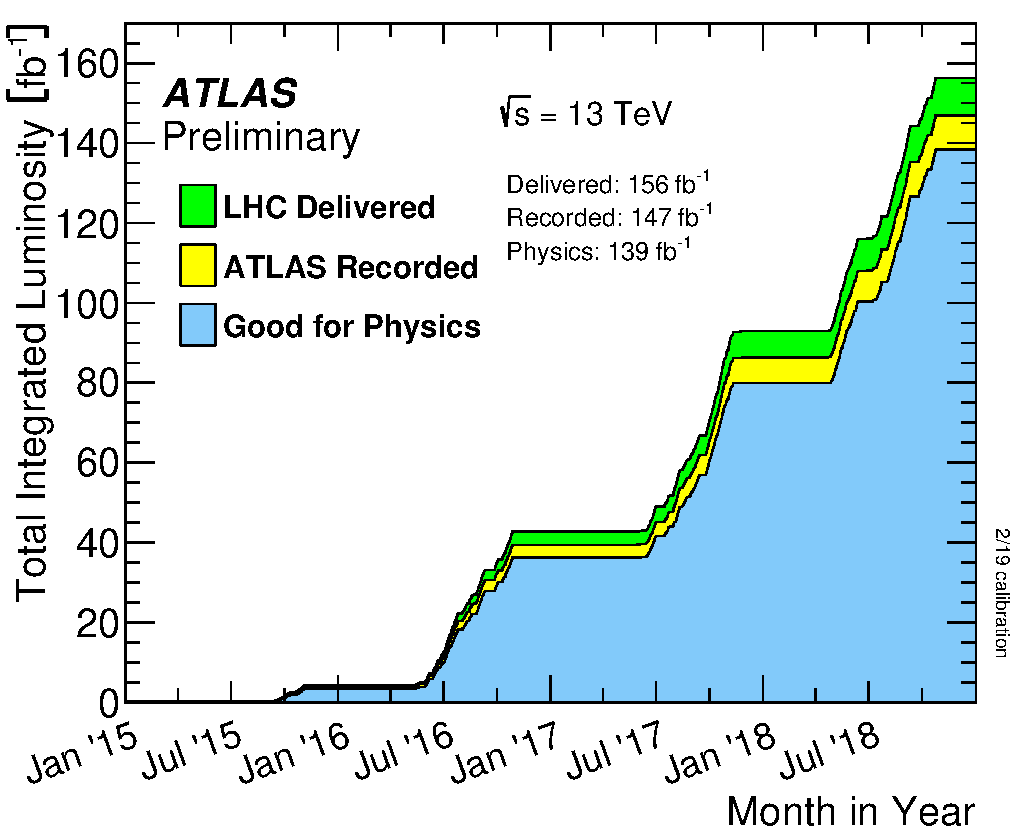
\includegraphics[width=\linewidth]{3_experiment/lhc/DeliveredLuminosityRun2}
        \caption{Run-2 (2015-2018)}
        \label{fig:atlas:runs:lumi_run2}
    \end{subfigure}
    \hfill
    \begin{subfigure}[h]{0.49\linewidth}
        \centering
        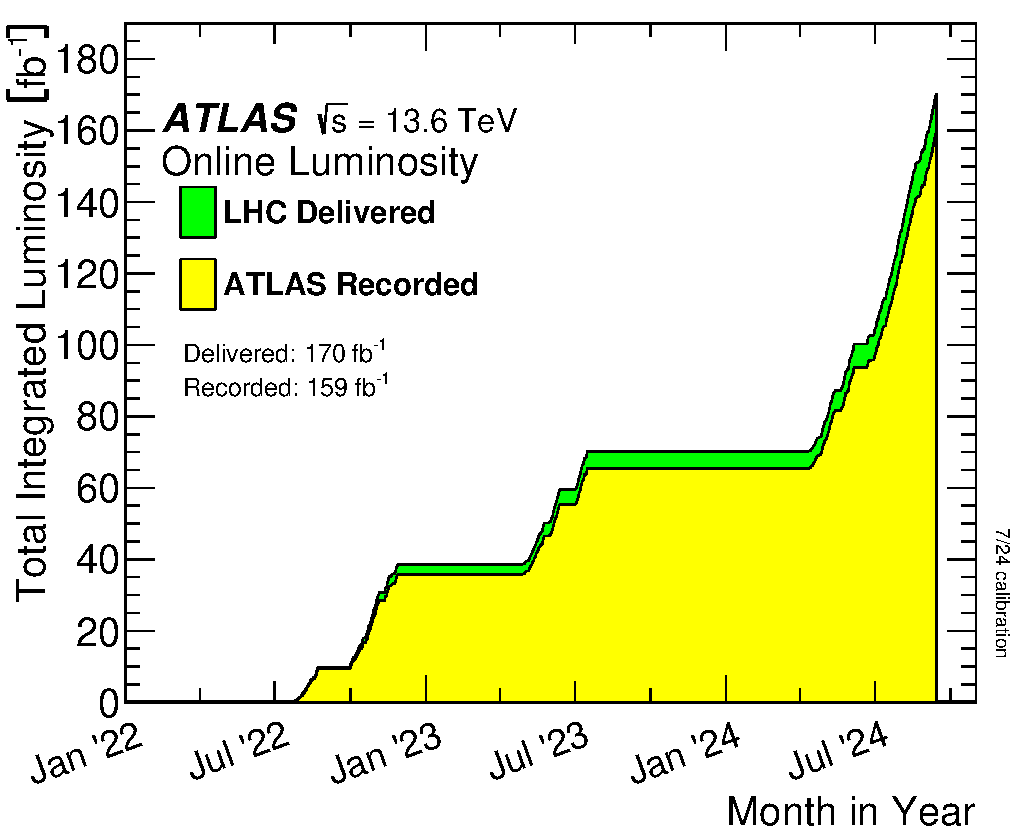
\includegraphics[width=\linewidth]{3_experiment/lhc/DeliveredLuminosityRun3}
        \caption{Early Run-3 (2022-2024)}
        \label{fig:atlas:runs:lumi_run3}
    \end{subfigure}
    \caption{Luminosity delivered by the \ac{LHC} and recorded by \ac{ATLAS} during the Run-2~\cite{ATLAS-Lumi-Run2} and Run-3 data taking periods. For Run-2, the fraction of data good for physics analyses is also displayed.}
    \label{fig:atlas:runs:lumi}
\end{figure}

Another important concept in \ac{ATLAS} data acquisition is pileup, which occurs when particles produced in more than one \pp collision arrive at the detector at the same time, or more generally, when signals overlap in a way that cannot be separated. When bunches of protons collide, the probability of an interaction is proportional to the particle density, or better, to the particle flux, which is expressed by the instantaneous luminosity. The actual number of particle collisions that take place when two bunches intersect is a random variable that follows a Poisson distribution. For low luminosities, in most beam crossings, no collisions occur, but for high instantaneous luminosities, in most crossings many particle collisions occur at the same time. Depending on the subdetector and the type of measurement, it may or may not be possible to distinguish between particles coming from different simultaneous interactions. This is called in-time pile-up. In contrast, out-of-time pile-up includes the effects that arise when the time the detector needs to return to its waiting state is longer than the time between bunches crossing. A quantitative measure of pile-up and event activity is the mean value of \pp inelastic interactions per bunches crossing, \avgmu.

The maximum instantaneous luminosities increased by a factor of four over the four years of Run-2, resulting in an increase of \avgmu from 10 up to 60, as shown in \Fig{\ref{fig:atlas:runs:pileup_run2}}. For Run-3, pileup was drastically increase up to values of 57 for year 2024, in average increasing up to 52 interactions per bunch crossing, displayed in \Fig{\ref{fig:atlas:runs:pileup_run3}}.

\begin{figure}[ht!]
    \centering
    \begin{subfigure}[h]{0.49\linewidth}
        \centering
        \includegraphics[width=\linewidth]{3_experiment/lhc/PileupConditionsRun2.png}
        \caption{Run-2}
        \label{fig:atlas:runs:pileup_run2}
    \end{subfigure}
    \hfill
    \begin{subfigure}[h]{0.49\linewidth}
        \centering
        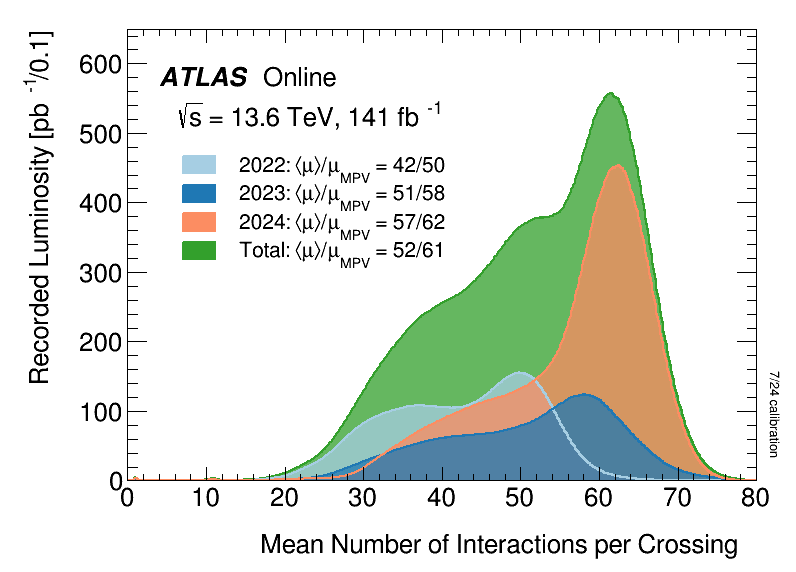
\includegraphics[width=\linewidth]{3_experiment/lhc/PileupConditionsRun3.png}
        \caption{Run-3}
        \label{fig:atlas:runs:pileup_run3}
    \end{subfigure}
    \caption{Pileup conditions during Run-2 and Run-3.}
    \label{fig:atlas:runs:pileup}
\end{figure}































































% \section{Monte-Carlo simulations}
% \label{sec:atlas:MC}

% The \acf{MC} method uses a series of computational algorithms based on the repetition of events with a variable and random factor, which allows obtaining global numerical results. In the context of particle physics, it is not only used to reproduce the randomness imposed by unique quantum mechanics, but also to perform different approximations, such as numerical integrals. \ac{MC} simulations play a fundamental role in the prediction of the theory, playing a key role in practically all the analyses carried out by the \ac{ATLAS} collaboration.

% After the event generation, the interaction between the particles and the detector is simulated. This is done using programs that simulate the passage of particles through matter, together with a full simulation of the \ac{ATLAS} detector, where the materials used and their dimensions are precisely detailed. This step is performed using the \GEANT4 software~\cite{Geant4} for full detector simulations.
% It is also possible to perform a simplified interaction simulation in order to save resources and computational time, called \textsc{AtlFast3}~\cite{AtlFast3}. Once the simulation of the detector has been performed, the events are reconstructed with the same algorithms used for data. Three simulation runs, \texttt{mc20a}, \texttt{mc20d} and \texttt{mc20e}, are generated with the expected pile-up distribution for data taken in the years 2015+2016, 2017 and 2018 respectively.























































% The \ac{LHC} \cite{LHCTDR,LHCMachine} is the largest particle accelerator in the world.  It is located at the \ac{CERN},  in Geneva,  Switzerland.  With its 27 km circumference, the accelerator ring is partially located in Switzerland and partially in France,  between 50-175 meters underground. 
% The \ac{LHC} was designed to accelerate protons in two separate beam pipes up to a centre of mass energy of 14 TeV.  It is also capable of accelerating heavy ions. 
% To keep the protons and heavy ions on the accelerator ring,  overall 9593 magnets are used.  These magnets include superconducting dipole and quadrupole magnets,  cooled down to 1.9 K (-271 $^{\circ}  C$).  The dipole magnets generate a magnetic field of 8.3 T. 

% \begin{figure}[htpb!]
% \centering
% \includegraphics[width=0.99\linewidth]{figures/ExpSetup/CernAcceleratorComplex2013.jpeg}
% \caption{Overview of the CERN accelerator facilities,  including the acceleration chain leading up to the \ac{LHC} \cite{CERNAcceleratorComplex2013} \label{fig:expSetup:acceleratorComplex}}
% \end{figure}

% Before the protons enter the \ac{LHC},  a chain of accelerators is used (see Fig.  \ref{fig:expSetup:acceleratorComplex}): starting from a hydrogen bottle,  negative hydrogen ions are fed into the Linear Accelerator 2 (LINAC2) and are accelerated up to 50 MeV.  Before getting inserted into the \ac{PSB} the ions are stripped of their electrons only leaving protons. The up to 2 GeV accelerated protons are then inserted into the Proton Synchrotron (PS),  followed by the \ac{SPS} which accelerates the protons from 60 GeV to 450 GeV before feeding the \ac{LHC}. Overall 8 radiofrequency cavities can push the energy of the protons in the LHC up to 14 TeV. 

% The \ac{LHC} so far provided proton and heavy ion beams for two data-taking periods.  Between 2009 and 2013 (known as Run-1), the LHC was operating with a centre-of-mass energy ($\sqrt{s}$) of 7 TeV and 8 TeV.  After a long shutdown (LS1) , the second run (Run-2) started in 2015 and ended in 2018,  providing 13 TeV collisions to the experiments around the \ac{LHC} ring.  In Figure \ref{fig:expSetup:acceleratorComplex} visualised yellow dots, there are four interaction points, housing the \acs{ALICE} \cite{ALICE},  \acs{LHCb} \cite{LHCb}, 
% \acs{CMS} \cite{CMS},  \acs{ATLAS} \cite{ATLAS}, \acs{LHCf} \cite{LHCf} , \acs{TOTEM} \cite{TOTEM}, \acs{MoEDAL} \cite{MoEDAL} experiments,  among many other experiments.

% The instantaneous luminosity \cite{LHCMachine} is a measure of the accelerator:

% \begin{align}
% \mathcal{L} = \frac{N_b^ 2n_bf_{rev}\gamma_r}{4\pi\epsilon_n\beta^*}F
% \label{eq:theory:instantaneousLumi}
% \end{align}
% With $N_b$ the number of particles per bunch,  the bunches per beam $n_b$,  revolution frequency $f_{rev}$,  the relativistic gamma factor $\gamma_r$,   $\epsilon_n$ normalised transverse beam emittance as well as $\beta^*$, the beta function at the collision point,  determining the transverse spread of the particle beam.  The correction term F takes into account the beam crossing angle. 

% \begin{align}
% N_{event} = L_{int} \sigma_{event} = \sigma_{event} \int \mathcal{L} dt \label{eq:theory:integratedLumi}
% \end{align}

% A measure for the recorded data is the integrated luminosity over time, (see equation \eqref{eq:theory:integratedLumi}), connecting the luminosity with the number of events.  This can be seen for each month during Run-2 in Figure \ref{fig:expsetup:LumiOverview}.  This illustrates the overall 156 $\text{fb}^{-1}$ of a proton-proton collisions delivered to \ac{ATLAS} by the \ac{LHC} as well as the 139 $\text{fb}^{-1}$  of data collected by \ac{ATLAS} with detector conditions good enough to use the events in data analysis.

% \begin{figure}[htpb!]
% \centering
% \includegraphics[width=0.75\linewidth]{figures/ExpSetup/DeliveredRecordedLumi.png}
% \caption{Summary of the luminosity delivered by the LHC,  recorded by the ATLAS detector as well as the overall data good to use for physics analyses \cite{LumiPublicResultsPage} \label{fig:expsetup:LumiOverview}}
% \end{figure}

% As already hinted to in equation \eqref{eq:theory:instantaneousLumi},  protons in the acceleration chain are accelerated in so-called bunches to generate high instantaneous luminosity.  
% As a consequence,  many proton-proton interactions can happen during one crossing of bunches.  In Figure \ref{fig:expsetup:pileup},  the mean number of interactions per bunch crossing is given for all years of Run-2 data-taking. This so-called \textit{pile-up} reached above 70 number of interactions per bunch crossing in 2017.  
% \begin{figure}[htpb!]
% \centering
% \includegraphics[width=0.75\linewidth]{figures/ExpSetup/PileupConditionsRun2.png}
% \caption{Pileup conditions throughout Run-2 \cite{LumiPublicResultsPage} \label{fig:expsetup:pileup}}
% \end{figure}







% %
% %\textcolor{gray}{
% %discuss accelerator chain - which energies in which accelerator 
% %some parts about magnet structure 
% %RF cavities for accelerations
% %include that the LHC is filled by single hydrogen bottle, its tilted to avoid water accumulating in the tunnel, magnet structure of the Lhc,  to focus beams and the RF cavities to accelerate.
% %}
% %.


% %include that the LHC is filled by single hydrogen bottle, its tilted to avoid water accumulating in the tunnel, magnet structure of the Lhc,  to focus beams and the RF cavities to accelerate.
% %Include some words on the bunch structure and the acceleration complex before the LHC. 
% %inlcude pileup discussion plot from lumi public results
% %integrated luminosity and instantaneous luminosity 
% %need to mention bunches, filling schemes to an extend, how often collisions are happening..
% %\textcolor{red}{have to mention what runs are - in connection with good runs lists}
% %\textcolor{red}{have to introduce run 1 and run 2 - because have run 1 analysis comparisons at some point? }





% %=====================================
% \FloatBarrier
% \section{ATLAS}
% \label{sec:ExpSetup:ATLAS}
% \FloatBarrier
% %=====================================
% The \ac{ATLAS} detector is located at Point 1 along the \ac{LHC}. This is the only \acs{CERN} site along the LHC ring with access to a main experiment, the \ac{SPS} as well as the LHC. 
% The overall structure is comparable to a barrel,  leading to the centre part of the detector being referred to as the barrel, as well as the large,  25m in diameter,  wheels on each side referred to as endcaps. 
% With its 25 meters tall and 44 meters length,  \ac{ATLAS} is the largest particle detector built on a collider so far. 
% It consists of multiple sub-systems and sub-detectors,  all built with different purposes in mind,  targeting momentum and energy reconstruction.  \ac{ATLAS} provides hermetic coverage around the beam axis,  enabling detection of all charged particles generated in the collisions in the plane orthogonal to the beam axis.  This is particularly important in searches for new physics, relying on analyses of momentum balances in the orthogonal plane such as discussed within this thesis.
% An illustration of the design of \ac{ATLAS} is given in Figure \ref{fig:expSetup:ATLASoverall}.  It is built up of multiple layers,  starting from the innermost component,  the \acf{ID},  providing tracking hits close to the beam pipe.  Surrounding the \ac{ID} is a system of two calorimeters. The outermost parts of \ac{ATLAS} are built by the muon spectrometer,  providing momentum reconstruction for muons passing through the inner detector layers. 
% Arguably one of the most striking features of \ac{ATLAS} is given through its magnet system.  Three superconducting Niobium-Titanium (NbTi) magnets span an overall length of 26m.  The first magnet system, the central solenoid,  is wrapped around the \ac{ID},  providing a 2 T axial magnetic field to curve the \ac{ID} tracks of charged particles. 
% The largest magnet parts are the eight barrel toroid coils,  intertwined with the outer muon system,  providing a total magnetic field of 4 T (0.5 T per coil) to measure the momentum of muons.  The toroid magnetic field is completed by the end-cap toroids,  also generating a magnetic field up to 4T for muons leaving \ac{ATLAS} close to the beam pipe. 

% \begin{figure}[htpb]
% \centering
% \includegraphics[width=0.9\linewidth]{../figures/ExpSetup/ATLAS_full.pdf} 
% \caption{Overview graphic of the ATLAS detector design \label{fig:expSetup:ATLASoverall},  with two people illustrated for scale reference \cite{ATLASfull}}
% \end{figure}

% Every component in \ac{ATLAS} working together enables the reconstruction and identification of a variety of particles with high precision.  An overview of the design capabilities of \ac{ATLAS} in terms of the momentum and energy resolution is given in Table \ref{tab:expSetup:Resolutions},  adapted from \cite{ATLAS}.
% Here the resolution given lists first a stochastic term,  measuring the uncertainty based on the statistically dominated interaction of a particle with the material,  followed by a noise term,  which accounts for uncertainties due to electronic noise in the readout process. 

% \begin{table}[htpb!]
% \includegraphics[width=\linewidth]{figures/ExpSetup/ResolutionATLASDesign.pdf}
% \caption{Performance goals of the \ac{ATLAS} detectors' subsystems.  Units are given in GeV.  $\bigoplus$ indicating a sum in quadrature of the single terms for the total uncertainty \label{tab:expSetup:Resolutions}\cite{ATLAS}. }
% \end{table}

% In the following, a brief overview of the detector is given; a more comprehensive description can be found in \cite{ATLAS} as well as the Technical Design Reports of the subsystems,  as cited throughout the description below. 

% \subsection{ATLAS Coordinate system}
% The coordinate system used within \ac{ATLAS} is used throughout this thesis and shortly described in the following \cite{ATLAS}. 
% The origin of the right-handed coordinate system is at the nominal interaction point,  with the positive x-axis pointing towards the centre of the \ac{LHC}.  The x-y plane is perpendicular to the beam axis,  defining the z-axis.  Towards the surface defines the positive y-axis.
% An azimuthal angle $\phi$ is defined around the beam axis, and a polar angle $\theta$ is the angle from the beam axis.  Instead of $\theta$ the rapidity $y$ is used for heavy objects:
% \begin{align}
% y = \frac{1}{2} \ln[(E+p_z)/(E-p_z)]
% \end{align}
% Differences in Rapidity are invariant under boosts along the beam axis.
% For massless objects or relativistic objects ($m << \vb*{p}$),  the pseudorapidity is used: 
% \begin{align}
% \eta = -\ln(\tan(\theta/2)) 
% \end{align}
% To quantify the distance between two objects,  $\Delta R$ is defined:
% \begin{align}
% \Delta R = \sqrt{\Delta\phi^2 + \Delta\eta^2} \label{eq:expsetup:deltaR}
% \end{align}
% The transverse momentum and energy are defined in the x-y plane,  with the transverse momentum given as $p_T = \sqrt{p_x^2 +p_y^2}$.

% %=====================================
% \subsection{Inner Detector}
% %=====================================
% A cross-section of the \ac{ID} system \cite{IDTDR} is shown in Figure \ref{fig:expSetup:InnerDetectors}, highlighting the distance of each subsystem from the beampipe. The innermost part of the \ac{ID}  is the \ac{IBL},  followed by three layers of pixel detectors.  At 299 mm radial distance from the beam pipe, four layers of \ac{SCT} modules are located before the \ac{TRT},  which extends the overall \ac{ID} detector size to a radius of 1082 mm.  The \ac{ID} allows for particle track reconstruction within $|\eta| < 2.5$.

% \begin{figure}[htpb!]
% \centering
% \subfloat[Sketch of the \ac{ID} and distances of its sub-detectors]{\includegraphics[width=0.49\linewidth]{figures/ExpSetup/ID_includingIBL.png}}
% \subfloat[Overview of barrel and end-cap \ac{ID} components, apart from \ac{IBL} \label{fig:expsetup:idendcaps}]{\includegraphics[width=0.49\linewidth]{figures/ExpSetup/ID_overview_noIBL.eps}}
% \caption{Slice view of the Inner Detector,  highlighting each sub-detectors distance to the beampipe \cite{IDsketchwithIBL} (a) and cut-out view of the barrel and endcap components,  not including the \ac{IBL} \cite{ATLAS} (b).  \label{fig:expSetup:InnerDetectors}  }
% \end{figure}
% \paragraph{IBL - Insertable B-layer}
% After Run-1,  during a long shutdown in 2013-2014,  the pixel detector system was subject to maintenance and upgrades.  Within this set of upgrades,  %the \ac{DBM} was inserted within the pixel detector volume,  
% a 4th pixel layer at a 3.3 cm distance from a new,  smaller beam pipe (33 mm outer radius,  originally 36 mm).  A fourth pixel layer was a first in particle physics experiments \cite{IBLTDR,IBLproceedings} and has led to significant improvements in interaction vertex reconstruction and identification of b-hadron jets. 

% \paragraph{Pixel Detector}
% The innermost pixel layer,  the IBL,  is surrounded by three layers of pixel detectors,  arranged in barrels around the beam pipe \cite{PixelDesignPerformance,PixelPerformanceProceedings}.  The first layer is at a distance of 50.5 mm from the beam pipe's centre.  As can be seen in Figure \ref{fig:expsetup:idendcaps},  the end caps of the pixel layer consist of 3 disks around the beampipe,  stretching the length of the pixel component of the \ac{ID} to 1.4 m length along the beam axis.  The pixel detector consists of overall 1744 pixel modules with a nominal size of $50 \mu m x 400 \mu m$ in the $(\phi, z)$ plane ($\phi, r$ for the disk panels), comprising over 80 million readout channels.  
% The pixel and \ac{IBL} part of the ATLAS detector is crucial for tracking,  providing 4 pixel hits over the entire \ac{ID} pseudorapidity coverage ($|\eta| < 2.5.$).  
% %The resolution in the barrel is 10 mm (R-f) and 115 mm (z),as in the end-cap.

% \paragraph{Semiconductor Tracker}
% The pixel detector and \ac{IBL} are located within \ac{SCT} modules \cite{SCT}.  
% Similar to the pixel detector modules, the \ac{SCT} modules are semiconductor-based,  arranged into cylindrical layers around the beampipe in the barrel region,  forming disks in the endcap.  Since the \ac{SCT} modules only provide precise location along one axis,  two modules are combined back-to-back and rotated against each other to gain two dimensional spacial information.  Four layers are arranged in the barrel,  nine disks in each endcap side (see Fig. \ref{fig:expsetup:idendcaps}). Including the endcap disks, the \ac{SCT} extends up to $|z| < 2735 mm$. 

% \paragraph{Transition Radiation Tracker}
% The last part of the \ac{ID} is the \ac{TRT} \cite{TRTDesignPerformance},  in the barrel stretching from 554 mm to 1082 mm radial distance.  This detector is composed of 4 mm diameter straw tubes,  arranged in parallel to the beam pipe or radially in the barrel and end-cap, respectively.  Within $|\eta| < 2.0$,  three barrel rings and 18 end-cap units provide typically 36 hits per track. The straws are intertwined with polypropylene fibres for passing through particles to create transition radiation.  Inside the straws is a thin tungsten wire,  collecting charges drifting through the straws gas mixture (Xe, CO2 and O2). The level of radiation and collected charges in each straw can be used to discriminate between electrons and charged pions.  The \ac{TRT} only offers spatial information in the $(R-\phi)$ plane, no information in the z-direction can be extracted due to the straws orientation. 
 
% %70% Xe, 27% CO2 and 3% O2.
% %R − phi direction, while no information is provided
% %along the z-direction.
% %and can provide up to 36 hits per track.
% %up the TRT are straw tubes 4 mm in diameter,
% %with walls made of two multi-layer films, each 35  m thick.
% %The TRT is designed to provide a large number of hits, typically 36 per track,
% %with a coverage of j j < 2:0. It has an intrinsic accuracy of 130  m in R 􀀀  ,
% %providing no information in the z-direction
% %The TRT [71] consists of three barrel rings, with 32 modules each, and 18 end-caps units
% %31 2.2 The ATLAS detector
% %with 224 layers.
% %These are positioned
% %parallel to the beam pipe in the barrel and radial in the end caps. The
% %n the TRT this is done by polypropylene
% %fibres (foils), which are interwoven between the barrel (end-cap) straws, that enable
% %the production of transition radiation in the formof X-rays. The amount of radiation
% %produced can be used to distinguish between, e. g. electrons and charged pions, as the
% %amount of radiation would depend on how relativistic the charged particle is.

% %The TRT can discriminate between two signals, according to their
% %amplitude: the lowest charge is due to the minimum-ionising particles (MIPs) crossing the
% %gas, while the strongest signal is given by the transition-radiation photons absorbed in
% %the gas. This last class of events is originated by the electrons, hence the TRT is able to
% %contribute to electron identification on a straw-by-straw basis
% %\subsubsection*{SCT - Semiconductor Tracker }
% %\subsubsection*{TRT - Transition Radiation Tracker}
% %
% %gaseous/polypropylene-fibre transition radiation tracker (TRT) a
% %\subsubsection*{BCM - Beam Condition Monitor} --> beam condition monitor
% %\cite{BCM}
% %=====================================
% \subsection{Calorimeter System}
% %=====================================
% The overall \ac{ID} system is surrounded by two sets of calorimeters \cite{ATLAS}.  An \acf{ECAL} \cite{LArTDR} in the inner most part, followed by a \ac{HCAL} \cite{TileTDR} (see Figure \ref{fig:expSetup:calorimeters}).  Both systems are designed to record the energy deposits of mainly electromagnetically interacting particles (electron,  photons) or the energy of hadrons,  based on hadronic interactions. 

% \begin{figure}[htpb!]
% \centering
% \includegraphics[width=0.75\linewidth]{figures/ExpSetup/Calorimeter_overview.eps}
% \caption{Illustration of the \ac{ATLAS} calorimeter system \cite{ATLAS} \label{fig:expSetup:calorimeters}}
% \end{figure}

% Both calorimeters are so-called sampling calorimeters with alternating layers of absorber and active material.  The absorber layer triggers a shower development of consecutive interactions with the detector material,  the active layer is detecting the signal. The shower development and properties can be a helpful characteristic in particle identification.
% Overall,  the calorimeters cover the $|\eta|$ range below 4.9.  Two important quantities in connection with the calorimeters are the radiation length, $X_0$,  and the interaction length $\lambda$.   The radiation length  refers to the distance after which an electrons energy has been reduced to 1/e of its initial energy.  The interaction length describes the mean free path before the occurrence of an hadronic interaction.


% \paragraph{Liquid Argon Calorimeter}
% Liquid Argon (LAr) calorimeters \cite{LArTDR} are used in multiple parts of the calorimeter system.  First,  it is comprising the \ac{ECAL},  with two half barrels covering the central detector region, with a small (4 mm) gap at $z = 0$ and one end-cap on each side of the beamline (see Fig. \ref{fig:expSetup:ecal}).  Additionally,  the LAr technology is used for the hadronic calorimeters end-caps as well as a \ac{FCAL} ($3.1 < \eta < 4.9$). 
% The active material is LAr,  with copper and kapton electrodes for readout.  The absorber is made of lead with stainless steel sheets.  As can be seen in Figure \ref{fig:expSetup:ecal},  an accordion symmetry is used to ensure homogeneous coverage all over $\phi$.

% \begin{figure}[htpb!]
% \centering
% \subfloat[\label{fig:expSetup:ecal}]{\includegraphics[width=0.45\linewidth]{figures/ExpSetup/ECalVis.png}}
% \subfloat[\label{fig:expSetup:crack}]{\includegraphics[width=0.45\linewidth]{figures/ExpSetup/CrackRegionmaterial.png}}
% \caption{Visualisation of an \ac{ECAL} slice at $\eta = 0$ (a),   next to an overview of the material in terms of radiation lengths infront of the presampler and main \ac{ECAL} (b).  Both from \cite{ATLAS}.}
% \end{figure}

% Infront of the \ac{ECAL} between $|\eta| < 1.52$ in the barrel region and $1.5 < |\eta| < 1.8$ in the end cap,  there is an additional layer of instrumented Liquid Argon,  the \textit{presampler}.  This is included in order to account for energy losses of particles before entering the \ac{ECAL}.  The first layer of the \ac{ECAL} has the finest granularity, comprising 4.3 $X_0$, followed by the second layer of 16 $X_0$ radiation lenghts in depth and a third layer with coarse granularity. 
% The total thickness in the barrel of the \ac{ECAL} is over 22 $X_0$,  over 24 $X_0$ in the endcap. 
% In Figure \ref{fig:expSetup:crack},  the amount of material infront of the presampler as well as the accordion part of the calorimeters is given in radiation lenghts.  Within the region of $ 1.37 < |\eta| < 1.52$,  a large amount of material is present.  This is due to the transition between the barrel and end-cap cryostats,  housing the calorimeters.  This region is knowns as the \textit{crack} region or transition region. 

% \paragraph{Tile Hadronic Calorimeter}
% The hadronic calorimeter is built of a tile calorimeter technology \cite{TileTDR} in the barrel and extend barrel region (between $0 < |\eta| < 1.7$,  see Figure \ref{fig:expSetup:calorimeters}).  Similar to the \ac{LAr} calorimeter the tile calorimeter is a sampling calorimeter,  with a steel absorber material as well as plastic scintillator tiles as active material.  The scintillator tiles are combined with optical fibres and photo-multipliers for signal readout.  In the barrel,  the tile calorimeter has an overall depth of roughly 9.7 interaction lengths. 

% %=====================================
% \subsection{Muon System}
% %=====================================
% The outermost part of the \ac{ATLAS} detector is the \ac{MS} \cite{MuonTDR}. It is embedded within the 4 T magnetic field generated by the barrel and endcap toroid magnets.  In Figure \ref{fig:expSetup:MS},  a quarter of the muon system is visualised, highlighting the different subsystems.  \acp{MDT} and \acp{RPC} form three layers around the barrel,  \acp{CSC} are used close to the beam pipe.  The \textit{Big Muon wheels},  forming the "lids" of the \ac{ATLAS} barrel structure,  are comprised of \ac{TGC} and \ac{MDT} subdetectors.  A short overview of the subsystems is given in the following.

% %d drift tube (MDT) and cathode strip (CSC) chambers for momentum determination an
% %resistive plate (RPC) and thin gap (TGC) chambers for triggering. The

% \begin{figure}[htpb!]
% \centering
% \includegraphics[width=0.8\linewidth]{figures/ExpSetup/MuonSpectrometer.png}
% \caption{Overview of a quarter of the muon spectrometer, showing all subsystems \cite{MuonTriggerPerformance} \label{fig:expSetup:MS}}
% \end{figure}

% \paragraph{MDT - Monitored Drift Tubes}
% The \ac{MDT} subdetectors of the muon spectrometer are drift tubes with a diameter of 29.97 mm.  They are filled with 93\% Ar,  7 \% CO2 and have a tungsten-rhenium wire in the middle.  There are in total 1171 \ac{MDT} chambers,  each layer with up to eight layers of drift tubes.  Overall 354240 tubes cover a pseudorapidity range up to $|\eta| < 2.7$,  providing high precision track coordinates perpendicular to the magnetic field.  In the innermost end-cap layer,  the \ac{MDT} chambers are replaced by \ac{CSC}'s. 

% %29.97 mm diameter drift tubes
% %93%Ar Å 7%CO2
% %tungsten-rhenium wire, measuring 50 ¹m in
% %Three to eight layers of drift tubes are used in
% %both barrel and end-caps to allow a total of twenty measurements for each track.\\
% %precision tracking
% %1171 MDT chambers, with a combined total of 354240 tubes.
% %ionisation
% %The coverage of the MDTs extends to
% %j j < 2:7 except in the innermost end-cap layer where they are limited to
% %j j < 2:0,
% %track coordinates
% %in the bending direction.
% %⌘| < 2.7.
% \paragraph{CSC - Cathode Strip Chamber}
% In the endcap in a pseudorapidity range of $2.0 < |\eta| < 2.7$,  the \ac{CSC} detectors provide a fast response and high spatial resolution,  similar to \ac{MDT}'s.  Since \ac{MDT} reach their maximum operational radiation tolerance close to the beampipe,  \ac{CSC} are used at the high radiation environment close to the beampipe.
% \ac{CSC} detectors are multiwire proportional chambers filled with the same gas mixture as \ac{MDT}'s.  They provide both $r$ and $\phi$ coordinates.
% %precision tracking
% %2:0 < j j < 2:7 replacing mdt's
% %incoming neutron
% %rate is expected to exceed 150 Hz=cm2, the maximum for safe operation of the
% %MDTs.
% %multiwire proportional chambers, using the same gas mixture
% %radial direction wire
% %characterised by a
% %fast response time and high spatial resolution
% %both radial and phi coordinate with
% Both \ac{MDT} and \ac{CSC} detectors are used for precision momentum measurements,  whereas \ac{RPC} and \ac{TGC} 
% detectors are used to provide fast information to the \ac{ATLAS} trigger system (see section \ref{sec:ExpSetup:trigger}).

% \paragraph{RPC - Resistive Plate Chambers}
% In combination with \ac{MDT}'s , \ac{RPC} detectors are used to provide a coarse,  quick,  secondary coordinate measurement.
% Each \ac{RPC} consists of two detector layers orthogonal to each other, providing $\phi$ and $\eta$ coordinate measurements.  The \ac{RPC} covers an overall pseudorapidity region up to $|\eta| < 1.05$.
% The detectors are named after the two resistive parallel plates of phenolic-melaminic plastic laminate within each chamber,  enclosing a gas mixture.
% %
% %triggering
% %provide a measure of the second coordinate in the
% %barrel.
% %They cover the pseudorapidity region |⌘| < 1.05.
% %much quicker response time compared
% %with the CSCs.
% %coarsely measure a second tracking coordinate in the
% %no-bending phi-projection to complement the
% %The chambers are filled with a gas mixture of C2H2F4 and a small fraction of resistive component
% %SF6 contained in two resistive parallel plates of bakelite, kept at a 2mm distance.
% %The two detector layers which form the chamber are placed orthogonally to read both the h and f
% %Two layers of chambers (middle station) provide the trigger for low-pT muons, while a
% %third one (outer station) is used for high pT trigger thresholds.

% \paragraph{TGC - Thin Gap Chambers}
% The last component of the \ac{MS} are \ac{TGC}.  They are multi-wire proportional chambers similar to \ac{CSC}'s,  but with a coarser granularity.  The gas filling is a mixture of CO2 and n-pentane (n-C5H12).  Similar to \ac{RPC} detectors,  \ac{TGC} are able to provide a signal faster than 25 ns,  allowing for a matchin of a signal to a specific bunch crossing.  Their fast readout time is used in the trigger system,  additional to \ac{MDT}, s they provide a secondary measurement of the azimuthal angle.   
% %triggering
% %TGCs are multi-wire
% %proportional chambers, filled with a mixture of CO2 and n-pentane (n-C5H12), and have a similar
% %structure as the CSCs but a higher granularity.
% %They are used as trigger chambers for muon tracks
% %and, in addition to the MDTs, they provide a second measurement of the azimuthal coordinate. Both
% %TGC and RPC chambers are designed to provide a signal over a time shorter than 25 ns.

% %=====================================
% %\subsection{Magnet System}
% %=====================================
% %\subsection{Forward Detectors}
% %%=====================================
% %%\subsubsection*{LUCID - Luminosity Cherenkov Integrating Detector}
% %%%\subsubsection*{AFP - ATLAS Forward Proton}
% %%\subsubsection*{ALFA - Absolute Luminosity For ATLAS}
% %%\subsubsection*{ZDC - Zero Degree Calorimeter}


% \FloatBarrier
% \subsection{The Trigger System}
% \label{sec:ExpSetup:trigger}
% %\subsubsection*{L1}
% %\subsubsection*{HLT}
% %\subsubsection*{MBTS - Minimum Bias Trigger Scintillator}

% With all the components of the ATLAS detector described above,  any interactions and electrical signals from the entire detector convolute into a large set of read-out information. Even without any proton-proton collisions provided by the \ac{LHC},  ATLAS can detect feedback from the detectors through for example cosmic muons. Storing every single interaction within ATLAS during collisions would exceed the storage capabilities of the CERN computing centres and simultaneous would not provide any differentiation between high energetic collision interactions and low energy scattering of the protons.
% The ATLAS trigger system has been designed to select collision events of interest to the multitude of physics analyses performed with ATLAS data.  To do so,  a two-stage trigger system was used during Run-2.  A visualisation of the trigger system, as well as the flow of data through this system, is given in Figure \ref{fig:expSetup:trigVis}.

% \begin{figure}[h]
% \centering
% \includegraphics[width=0.8\linewidth]{figures/ExpSetup/triggerSystem_withoutFTK.pdf}
% \caption{Overview of the ATLAS trigger system during Run-2.  Adapted from \cite{Run2TriggerOperation} \label{fig:expSetup:trigVis}}.
% \end{figure}

% The first trigger level is based in hardware.  This \textit{Level-1} trigger is built of processors digitizing the calorimeter readout and information from the muon spectrometers (\ac{TGC}, \ac{RPC}),  identifying electrons, photons,  tau leptons,  jets,  and can calculate missing transverse energy.  The L1Topo component of the Level-1 system allows for topological requirements such as invariant mass selections and distance measures to be taken into account in the Level-1 decision.  The final decision to keep or discard an event at Level-1 is made by the \ac{CTP}.  This Level-1 trigger step reduces the 40 MHz collision rate down to a maximum rate of 100 kHz \cite{Run2TriggerOperation} and passes on Regions-of-Interest in $\eta$ and $\phi$ to the next trigger step,  the \acf{HLT}.  Regions-of-Interest consist of neighbouring calorimeter cells in the \ac{ECAL} and \ac{HCAL},  a detailed discussion in connection with electron triggers is given in Chapter \ref{ch:trigger}.\\
% The \ac{HLT} is a software-based trigger,  a computing farm allowing for sequences of algorithms.  The \ac{HLT} is designed to reduce the event rate from 100 kHz to around 1 kHz that is saved.  The algorithms run on the \ac{HLT} farm have access to higher granularity calorimeter information as well as tracking information from the \ac{ID}.  A typical trigger sequence includes fast algorithms, designed to quickly reject events not targeted by the trigger,  followed by more precise algorithms that can run more time-consuming reconstruction and identification similar to events stored offline.  The exact sequence and type of algorithms considered at the \ac{HLT} are defined in the trigger \textit{menu}.  This comprises a database of triggers,  each trigger defining a sequence of algorithms and requirements on these algorithms for an event to pass the \ac{HLT}.  
% The overall set of triggers targeting various detector signatures associated with particles,  such as electrons,  muons or photons as well as missing transverse energy.  The trigger requirements are designed and budgeted in a way that the overall \ac{HLT} rate does not exceed 1 kHz. 
% In some cases,  even the reduction in event rate achieved through the \ac{HLT} algorithms for desired trigger requirements,  such as low momentum triggers,  is too high.  To keep the overall \ac{HLT} rate below 1 kHz in these cases,  triggers can still be included in the menu, but with a \textit{prescale}.  A prescale is an artificial scaling of the trigger,  only accepting every Nth trigger decision if the prescale factor is N.  This allows triggers with an otherwise high rate to still collect events.
% %\textcolor{red}{need to mention what trigger towers are}
% %\textcolor{red}{have mentioned the bandwidth and budgets of the different signatures? -- might have built up to this in the DAQ section}



\chapter{Reconstruction and identification of physical objects}
\label{ch:objects}
\epigraph{\emph{“Champions keep playing until they get it right.”}}{Billie Jean King}


The particles (and products of their decays) produced at every collission, interact with the detector in a particular manner according to their nature. The information recollected by all the sub-detectors described in the previous chapter allow for the reconstruction and identification of the physical objects present in each accepted event by the trigger system. Two types of reconstruction and identification exist. The \textit{online} one, is carried out at the same time the \pp collissions take place, and the \textit{offline} one, done after the events are saved to storage. The reconstruction is done event by event, and is carried in the same way for events recorded by the \ac{ATLAS} detector and for simulated \ac{MC} events. In the following, a brief overview of the offline reconstruction and identification of the objects used in this thesis is given.



\fixme{update chapter, see version in spanish}



\section{Track and vertex reconstrucion}

In a high-pile-up event, there can be of the order of 1000 charged particles passing through the \ac{ATLAS} detector. The information from the \ac{ID} (\Sect{\ref{subsec:atlas:atlas:id}}) is used to reconstruct the trajectories of charged particles, called \textit{tracks}.

Tracking charged particles is a critical step in reconstruction. Tracks encode charged particles' momentum and trajectory, playing an essential role in particle identification and primary vertex reconstruction. As the inner detector is closest to the beamline and comprises minimally ionizing detector material with high granularity, it plays the main role in track reconstruction. A charged particle passing through different layers of \ac{ID} leaves a signal via ionization. As the \ac{ID} solenoidal field is homogenous, the resulting trajectory is circular in the \(xy\) plane. Five parameters shown in \Fig{\ref{fig:objects:track_vtx:track_parameters}} define charged particle tracks:
\begin{itemize}
    \item \(q/\pt\): the ratio of the charge and transverse momentum defining the curvature
    \item \(d_0\): the distance of the closest approach to the primary vertex in \(xy\)-plane defining the transverse impact parameter
    \item \(z_0\): the longitudinal impact parameter along the \(z\)-axis
    \item \(\phi_0\): the azimuthal angle
    \item \(\theta_0\): the polar angle of the particle direction oat the closest point of approach~\cite{ATLAS-Tracks-Performance-Run2}.
\end{itemize}

\begin{figure}[ht!]
    \centering
    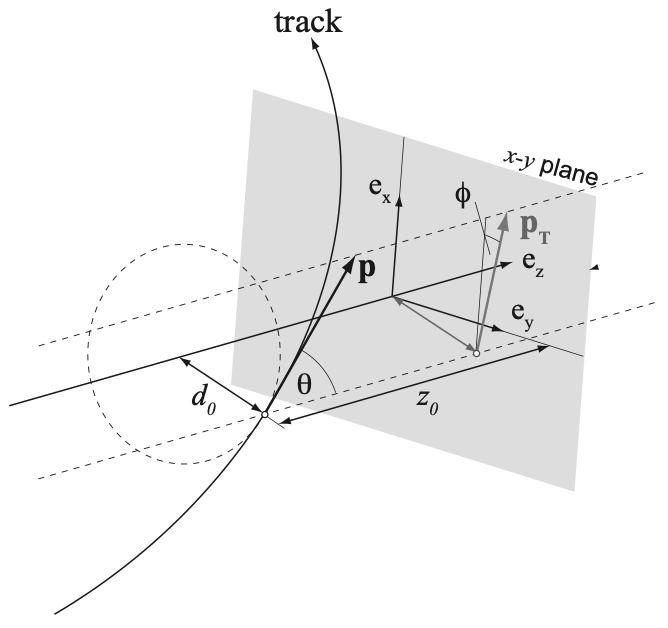
\includegraphics[width=0.6\linewidth]{3_experiment/object_reconstruction/tracking_coordinates.png}
    \caption{Schematic showing the tracking parametrization~\cite{ATLAS-Tracking-2007}.}
    \label{fig:objects:track_vtx:track_parameters}
\end{figure}

The track reconstrucion used in Run-2 uses two complementary approaches: the \textit{inside-out} approach, and the \textit{outside-in}~\cite{ATLAS-NEWT}. 

The first step in the inside-out track reconstruction is the seed-finding, where three hits in the silicon detector are searched for to seed the track reconstruction. Using these three hits and assuming an uniform magnetic field, a first estimate of the track parameters is obtained. Using the track seeds, the track is extrapolated to the other silicon layers, from which a combinatorial Kalman filter is used to estimate the track parameters. At this stage of the process there can be several track candidates for each track seed. Once the track is formed, an ambiguity resolution algorithm is applied to reassign shared clusters to the track with a better match~\cite{ATLAS-NNClustering}, and the final track candidate is fitted using a global \chisq method. The last part of the inside-out method consists on extending the tracks to the \ac{TRT}, and including the \ac{TRT} hits to the track, to improve the track's momentum resolution.

To improve the efficiency for tracks from decays displaced from the original collision point, an outside-in track reconstruction algorithm is also used. The track is seeded with hits from the \ac{TRT}. The track is extended to include hits from the silicon detector, with an ambiguity solver again applied to mitigate the hit sharing between two tracks.

Primary and secondary vertices are of vital importance for the subsequent object reconstruction in \ac{ATLAS}. In this step, the tracks found as explained previously are used as input to the vertexing algorithm~\cite{ATLAS-PVReconstruction,ATLAS-VertexReconstruction}. First of all, the \ac{PV} is defined as the location where two protons collide. \acp{PV} are reconstructed by matching up intersecting tracks, which proceeds in three main steps: seeding, track assignment, and fitting. The vertex with the largest \(\sum \pt^2\) for all associated tracks is labeled as the hard-scatter vertex. There are some particles that decay rapidly after their production, such as \(\tau\) leptons or heavier quarks (\(b\) or \(\cquarks\)), and their decay position can be measured. From the remaining tracks originated from these decays, it is possible to identify secondary vertices. All the remaining reconstructed vertices are considered to be pile-up.








\section{Photons and electrons}

The reconstruction of electrons and photons in \ac{ATLAS} is based on the energy deposition in the \ac{ECAL}. Since electrons and photons leave similar signals in the \ac{ECAL}, their reconstrucion is done simultaneously, distinguishing between them by the reconstructed track information left in the \ac{ID}.


\subsection{Reconstruction}
\label{subsec:objects:egamma:reco}

The \textit{offline} photon and electron reconstruction~\cite{ATLAS-EGamma-Performance-2015-2017,ATLAS-TopoClusters-Run2} makes use of dynamic, variable-size clusters, connected topologically between the \ac{ECAL} and \ac{HCAL} cells~\cite{ATLAS-TopoClusters-Run1}, called topo-clusters. This approach allows for the clusters to recover energy from bremsstrahlung photons or from electrons from photon conversions. With this approach, there are three types of objects:
\begin{itemize}
    \item Electrons: consists of a cluster built from the energy deposits in the \ac{ECAL} and a matched track.
    \item Converted photons: consits of a cluster mathed to a conversion vertex (or vertices)
    \item Unconverted photons: cluster matched to neither an electron track nor a conversion vertex.
\end{itemize}

\begin{figure}[ht!]
    \centering
    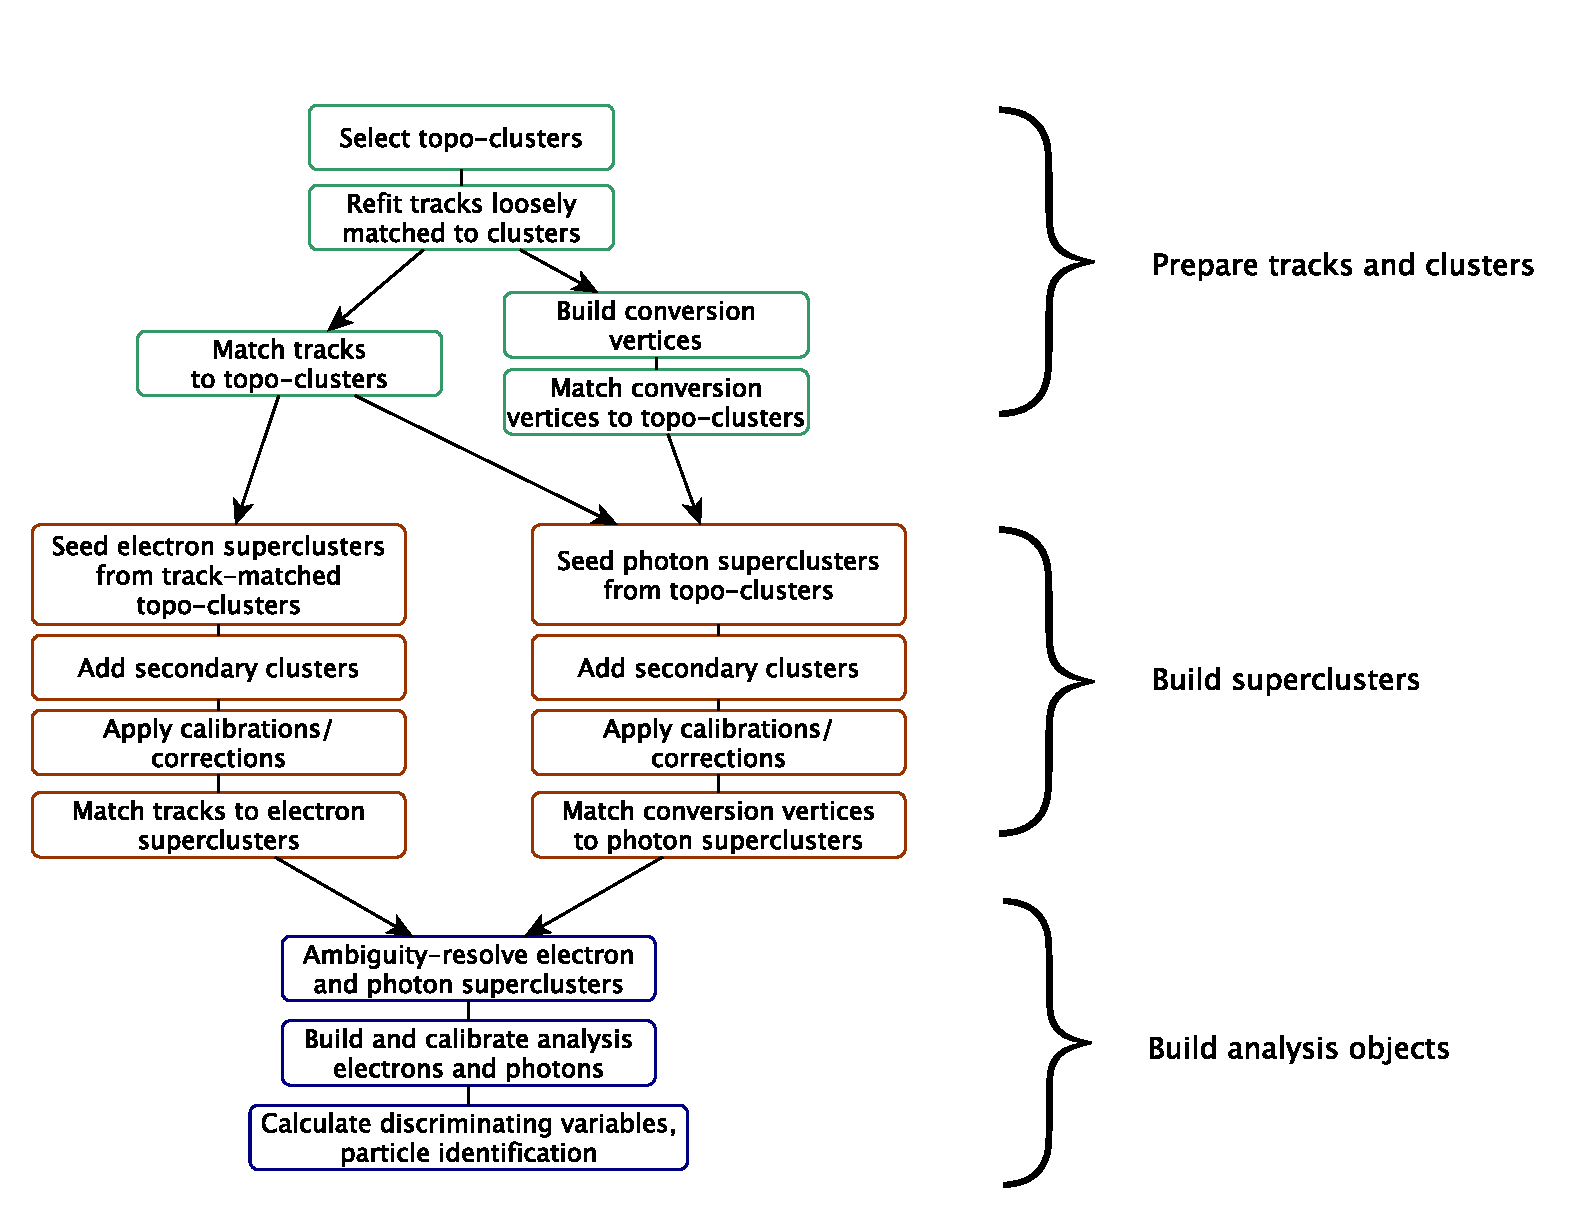
\includegraphics[width=0.8\linewidth]{3_experiment/object_reconstruction/egamma_reconstruction}
    \caption{Diagrama showing the reconstruction algortihm workflow for electrons and photons, extacted from \Refn{\cite{ATLAS-EGamma-Performance-2015-2017}}}
    \label{fig:objects:egamma:reco:reco_diagram}
\end{figure}

The algorithm for the reconstruction of electrons and photons proceeds as shown in \Fig{\ref{fig:objects:egamma:reco:reco_diagram}}.
The reconstruction process begins with the topo-cluster formation. First, proto-clusters are formed in the \ac{ECAL} and \ac{HCAL} by grouping cells that have a required energy, and by subsequently adding neighbouring cells in four consecutive steps, obtaining the topo-cluster. Reconstructions starts only in those cases where the topo-clusters energy in the \ac{ECAL} is greater than \(400~\mev\).

The algorithm also builds conversion vertices out of the refitted tracks and matches them to the selected topo-clusters.
After the initial track-cluster matching and conversion building, the electron and photon supercluster algorithms run separately in parallel. In the first stage, topo-clusters are evaluated for use as seed cluster candidates, which form the basis of superclusters; in the second stage, clusters near the seed candidates are identified as satellite cluster candidates, which may emerge from bremsstrahlung radiation or topo-cluster splitting. Satellite clusters are added to the seed candidates to form the final superclusters, if they pass the necessary selection criteria.
After applying initial position corrections to the resultant superclusters, the reconstruction algorithm matches tracks to
the electron superclusters and conversion vertices to the photon superclusters.

Since one object may be reconstructed as both an electron and a photon, an ambiguity resolution is performed to remove part of the overlap. However, some overlap is allowed in order to maintain a high reconstruction efficiency for electrons and photons, to which physics analyses may apply their own criteria. The final electrons and photons are then built and calibrated, facilitating the calculation of additional variables used for quality cuts and ambiguity resolution



\subsection{Identification}
\label{subsec:objects:egamma:id}

In order to distinguish real photons (those coming from the collision) from background photons which have much larger production cross sections (coming from hadrons decays, also called fake photons), it is necessary to rely on a algorithm of identification with high signal efficiency and background rejection, for photon candidates with \(\pt \sim 10~\gev\) up to the \tev scale. 
Currently, photon identification in ATLAS is based on a set of rectangular cuts on \acp{SSV} computed from the energy deposited in the cells of the cluster in the first and second layer of the \ac{ECAL}, and from the leakage to the \ac{HCAL}. These variables describe the passage of the photons through the calorimeters, characterizing the lateral and longitudinal electromagnetic showers.
The full photon identification process is presented in \Ch{\ref{ch:pid_ss}}, where the \acp{SSV} are explained one by one. Also, \Chs{\ref{ch:ffs}}{\ref{ch:cellrw}} present two approaches to correct the differences seen in these \acp{SSV} between data and \ac{MC}.



\subsubsection{Shower shape variable corrections}

Due to the imperfection of the \ac{ATLAS} simulation to model the \acp{SSV}, and that these variables are used as input to the identification step, it is important that they are corrected. Historically, the corrections are called \acp{FF}, and they comprised modifications to the mean value of the \acp{SSV}, calculated by minimizing the \chisq value between the data and \ac{MC} \acp{SSV}.
More details on the \ac{SSV} corrections are given in GIVE SECTION!!!

Additional corrections to all the reconstructed and identified photons in the simulation are applied event-by-event in the form of scale factors. These values, provided centrally by the \textsc{EGamma} group to \ac{ATLAS}, represent the residual differences on the efficiencies between actual data and \ac{MC}, computed as a function of the photon \pt and pseudo-rapidity \(\eta\) and separately for converted and unconverted photons.








\subsection{Isolation}
\label{subsec:objects:egamma:iso}

To further reduce the backgrounds of jets misidentified as photons and of hadron decay within the jets (such as the case of neutral pions), two isolation variables are defined: \etconefo and \ptconetw.

\begin{figure}[ht!]
    \centering
    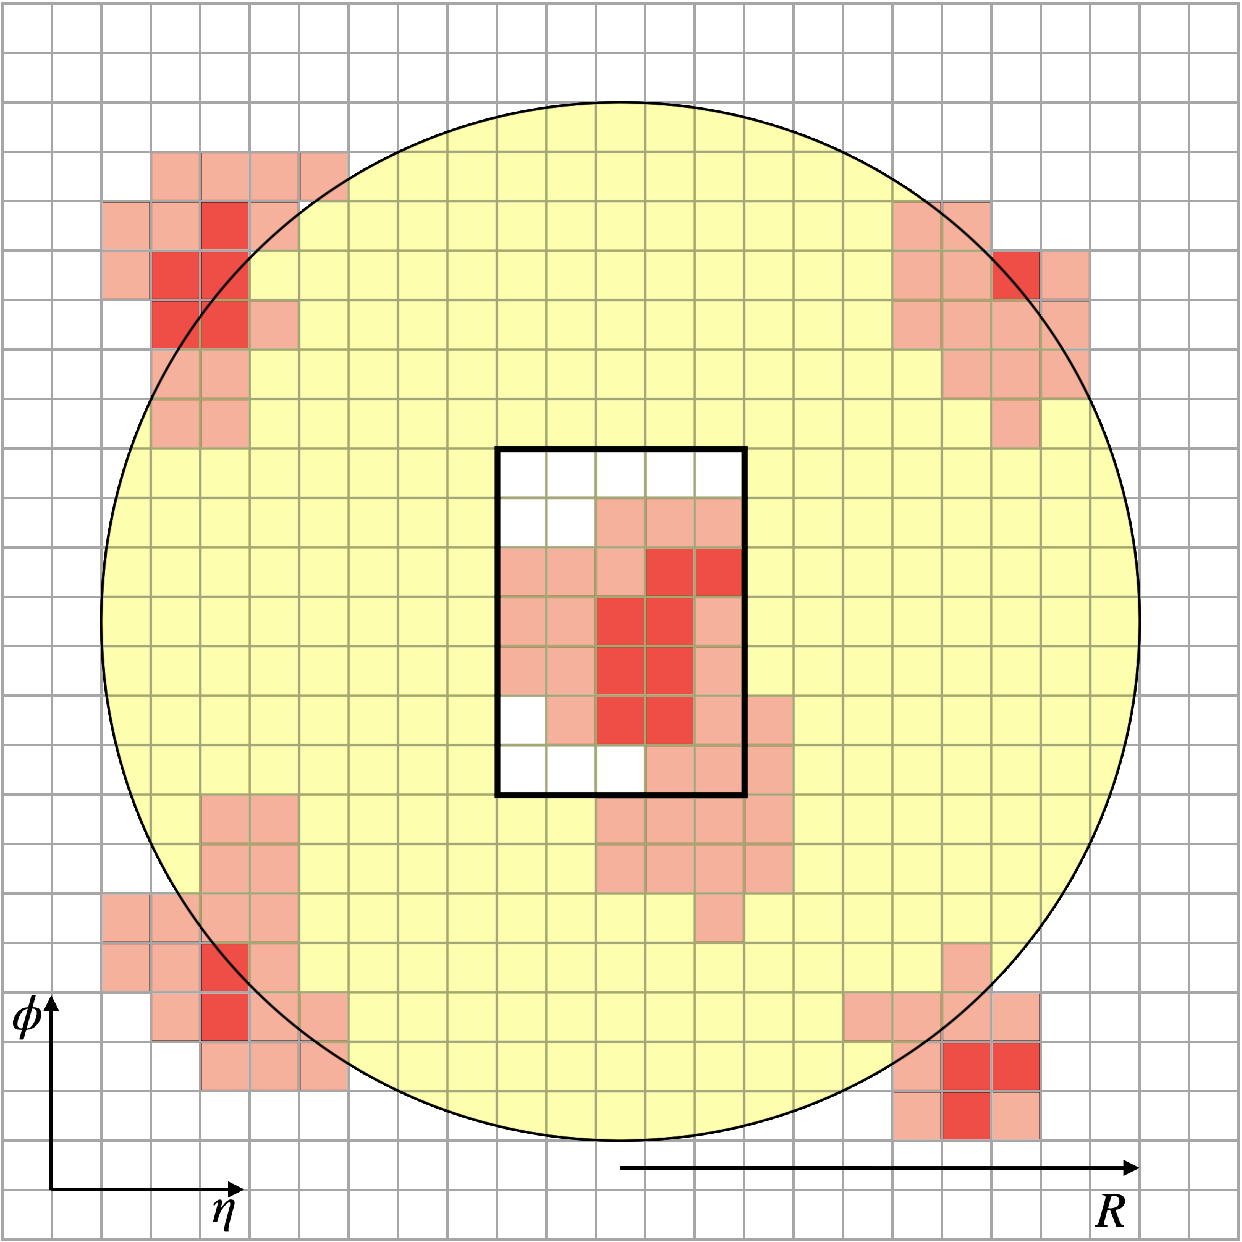
\includegraphics[width=0.5\linewidth]{3_experiment/object_reconstruction/isolation_diagram}
    \caption{Diagram showing the calculation of the calorimetric isolation variable. When \(R=0.4\), \etconefo is computed.}
    \label{fig:objects:egamma:iso:iso_diagram}
\end{figure}

The procedure to compute the isolation energy \etconefo is as follows, and showed in \Fig{\ref{fig:objects:egamma:iso:iso_diagram}}. First, a cone of radius \(\DeltaR<0.4\) is built around the photon or electron candidate, and the energies of all the cells in the topo-clusters (introduced in \Sect{\ref{subsec:objects:egamma:reco}}) whose bary-centers are located inside the cone, are added together. Then, to this computed energy, the energy of all the cells in a \(5\times 7\) window (in units of \(\eta \times \phi\) in the second layer of the \ac{ECAL}) centered around the candidate are subtracted, in order to remove the energy of the candidate itself. Pile-up contributions and energy leakages outside the cone are also taken into account.

The track isolation variable \ptconetw is obtained by adding the \pt of the good-quality tracks in a cone of radius \(\DeltaR<0.2\) around the electron candidate or in the direction of the converted photon cluster.
The track associated to the track or to the converted photon are excluded from this computation, as well as those tracks which do not pass the \textit{good-quality} track requirement. A \textit{good-quality} track is defined as one in which the \pt is \(\pt>1~\gev\), and it has a minimum distance to the primary vertex along the \(z\)-axis of \(|z_0 \sin \theta| < 3\) mm.

In general, for photons and electrons, there is no other energy deposited in the cone around the candidate, apart from the low-energy objects originating from the remnants of the collision, multiple interactions and pile-up. On the other hand, for fake photon candidates and non-direct photons, additional energy is observed within the cone, originating from objects accompanying the jet.

\begin{table}[ht!]
    \caption{Summary of electron and photon isolation \acp{WP} use throughout this thesis.}
    \resizebox{\linewidth}{!}{%
        \begin{tabular}{|l|c|c|c|}
            \hline
            Object                      & WP                             & Calorimetric Isolation                                    & Track Isolation   \\ \hline
            \multirow{3}{*}{Photon}     & \texttt{FixedCutLoose}         & \(E_{T}^{\text{cone20}}<0.065\times \pt \)                & -                                  \\
                                        & \texttt{FixedCutTightCaloOnly} & \(\etconefo < 0.022\times \pt + 2.45~\gev\)               & -                                  \\
                                        & \texttt{FixedCutTight}         & \(\etconefo < 0.022\times \pt + 2.45~\gev\)               & \(\ptconetw/\pt < 0.05\)           \\ \hline
            \multirow{2}{*}{Electron}   & \texttt{Loose\_VarRad}         & \(\etconetw < 0.2\times\pt\)                              & \(\pt^{\text{cone30}}/\pt < 0.15\) \\
                                        & \texttt{HighPtCaloOnly}        & \(\etconetw < \max\left(0.015\times\pt, 3.5~\gev\right)\) & -                                  \\ \hline
        \end{tabular}
    }
    \label{fig:objects:egamma:iso:iso_table}
\end{table}

From the calorimetric and track isolation different \acp{WP} can be defined separately for both electrons and photons. For electrons, two strategies are defined: either to achieve a fixed effiicency, or to apply fixed cuts on the isolation variables. In the case of photons, there are \acp{WP} which do not use both the isolation variable, as is the case of the \texttt{FixedCutTightCaloOnly} \ac{WP}, which only uses calorimetric isolation. The definitions of the different \acp{WP} used throughout this thesis is shown in \Tab{\ref{fig:objects:egamma:iso:iso_table}}. Also, it is common to define the following variables for the photon \texttt{FixedCutTight} \ac{WP}:
\begin{align}
    \etiso &= \etconefo - 0.022 \times \et - 2.45~\gev\\
    \ptiso &= \ptconetw / \et
\end{align}
therefore leaving the \texttt{FixedCutTight} \ac{WP} defined as
\begin{align}
    \etiso &< 0 ~\gev\\
    \ptiso &< 0.05 
\end{align}















\section{Muons}



The rate of bremsstrahlung radiation is inversely proportional to the square of a particle's mass. Since muons are about 200 times heavier than electrons, they primarily interact with the detector material through ionization. Therefore, muons are minimally ionizing particles that do not create electromagnetic shower in the calorimeters and pass through all layers of the \ac{ATLAS} detector. Hence, muon detection relies on track measurements from the \ac{ID} and \ac{MS}. The combination of the two subdetectors define four types of muons, depending on the used information for the reconstruction:
\begin{itemize}
    \item \acp{CB}: muons reconstructed from a global refit of \ac{ID} and \ac{MS} tracks
    \item \acp{ST}: muons reconstructed from a fitted \ac{ID} track and \ac{MS} segment track
    \item \acp{CT}: muons reconstructed using \ac{ID} track matched to the minimum ionizing energy deposits in the calorimeters
    \item \acp{ME}: muons reconstructed solely from \ac{MS} tracks.
\end{itemize}


The overlap between different types of muons is resolved as follows. When two muon types share the same \ac{ID} track, the order of preference is: first \ac{CB}, then \ac{ST} and finally \acp{CT}. The overlap with \acp{ME} is solved by analyzing the hits of the tracks, selecting those tracks with the best fit and the highest number of hits.

For the muon identification, quality cuts are applied to distinguish isolated muons from those coming from background processes, mainly from pion and kaon decay.
The variables with good discriminating power used are described in \Refn{\cite{ATLAS-Muon-Performance-2016}}. Four identification selections are defined: Loose, Medium, Tight, and High-\pt. The first three categories are inclusive, and Medium being the default selection in \ac{ATLAS}. Finally, the muon candidates to be used by the analyses are asked to satisfy the isolation requirements, both at traack and calorimetric levels, analogously to what was detailed for photons in the previous section. For the first case, a variable similar to that used for photons is used, but with a variable-radius cone \(\DeltaR = \min(10~\gev/\pt, 0.3)\) around the muon \pt, excluding the muon track. For calorimetric isolation the same variable \etconefo is used, with the difference of using a radius of \(R=0.2\), instead of \(0.4\) as before. Based on these variables, 7 isolation selection criteria (7 \acp{WP}), optimized for different analyses, are defined.








\section{Jets}


Due to color confinement in \ac{QCD}, a quark or gluon cannot exist on its own and goes through hadronization to form a collimated color-neutral stream of particles, \textit{jets}. Generally, jets penetrate through the \ac{ECAL} and get fully absorbed by the material in the hadronic calorimeter. In the following, a brief description of the typical clustering method adopted by \ac{ATLAS} is given. Also, the two existing types jet reconstruction are described.


\subsection{\Antikt jet clustering algorithm}

Given that jets are constituted by a high number of particles that leave energy depositiions in the \ac{ECAL} and \ac{HCAL} and tracks in the \ac{ID}, a clustering algorithm groups together constituents in the event to define the jets. Said algorithm is called the \antikt algorithm~\cite{AntiKtAlgorithm}. In the same way as for electrons and photons, \ac{ATLAS} jet reconstruction relies on the formation of \topos: grouped energy depositions in the calorimeters cells using a sequential combination algorithm. Then, the \antikt algorithm combines the \topos with the following steps:
\begin{itemize}
    \item Measure the distance between all \topos between themselves, and of each \topo with the beam:
        \begin{gather}
            \dij = \min \left( p_{T,i}^{-2}, p_{T,j}^{-2} \right) \frac{\Delta_{i,j}^2}{R^2}\\
            d_{iB} = p_{T,i}^{-2}
        \end{gather}
        where \(\Delta_{ij}^2 = \Delta\phi_{ij}^2 + \Delta\eta_{ij}^2\) and \(R\) is the jet-radius.
    \item If the minimum of all the distances computed previouly is \(d_{iB}\), the \topo \(i\) is classified as a jet, and is discarded in successive iterations.
    \item If the minimum of all the distances is \(d_{ij}\), \topos \(i\) and \(j\) are combined, all the distances are computed again with this new \topo and the iteration is carried all over again.
\end{itemize}
This process is repeated until all te particles in the event have been clustered.

The \antikt algorithm starts by clustering the radiation around the hardest particle in the event since the leading \pt particle will define the \(\min \left( \frac{1}{p_{T,i}^2}, \frac{1}{p_{T,j}^2}  \right)\) term in the \dij definition. This allows jets in the event to have a stable direction early on the combination process. The \antikt algorithm is preferred to other sequential jet algorithms since jets have regular boundaries which are approximately conical, shown in \Fig{\ref{fig:objects:jets:antikt}}. Jets originating from quarks or gluons in general are called small-\(R\) jets and a radius of \(R=0.4\) is used for their reconstruction. On the other hand, jets representing massive particles which decay hadronically are called large-\(R\) jets, and use \(R=1.0\). The usage of a wider cone helps to include the majority of the particles product of the decay.


\begin{figure}[ht!]
    \centering
    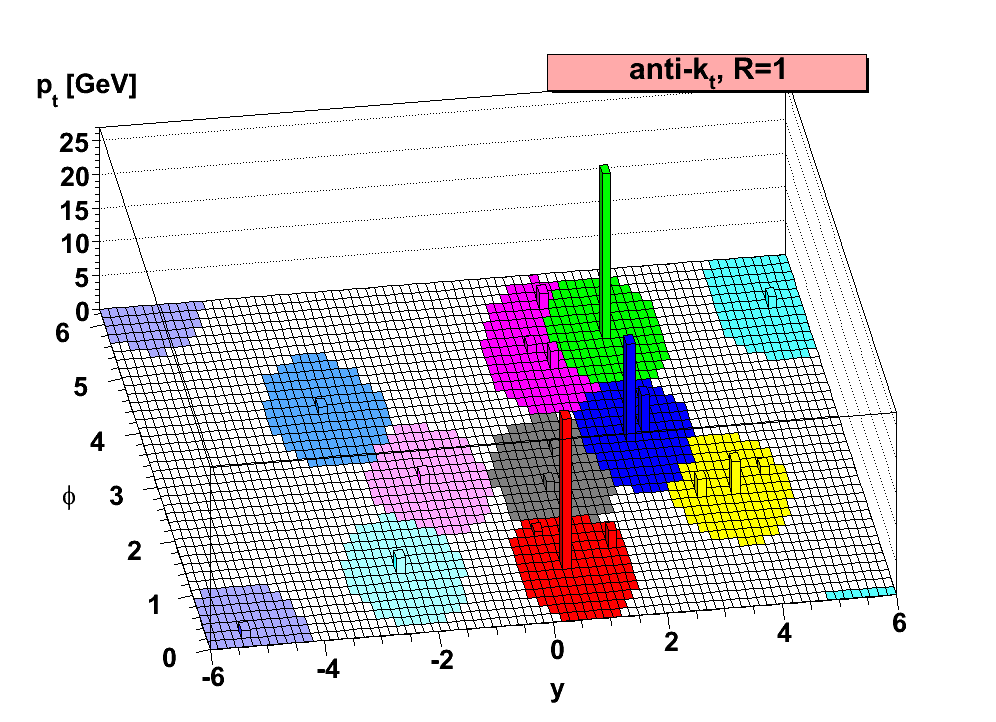
\includegraphics[width=0.7\linewidth]{3_experiment/object_reconstruction/antikt_clusters}
    \caption{Schematic representation of the \antikt algorithm for jet clustering~\cite{AntiKtAlgorithm}.}
    \label{fig:objects:jets:antikt}
\end{figure}

\subsection{Calorimeter Jets}

One way to reconstruct jets is based on energy deposits in the calorimeter. In a similar way to what has been explained for electrons and photons in \Sect{\ref{subsec:objects:egamma:reco}}, energy depositions on the cells of the \ac{ECAL} and \ac{HCAL} are used to build \topos, which approximates the energy deposits of individual hadrons~\cite{ATLAS-TopoClusters-Run1,ATLAS-TopoClusters-Run2}. Jets reconstructed in this manner and clustered with the \antikt algorithm with a radius of \(R=0.4\) are referred as \textsc{EMTopo} jets, and are the proxies for the individual quarks and gluons. In the jet reconstruction, only the \topos with positive net energy are included.

\subsection{PFlow Jets}

Another approach for jet reconstruction is taken in the particle flow algorithm, in which measurements from both the tracker and the calorimeter are combined to form the signals, which ideally represent individual particles.
In this alorithm, tracks are matched to \topos using proximity in \((\eta,\phi)\) space, also accounting for the size of the \topo. The tracks are only “matched” if the cluster carries more than \(10\%\) of the track's momentum. Sometimes the \topo fails to cluster all of the hadron's energy in a single \topo. In cases where the expected energy of the track is less than the expected track's energy, a “split shower recovery” combines nearby \topos to form a \topo set. From this \topo set, the expected energy of the track is subtracted from the \topo's cells, starting with high-energy density cells. If the residual energy is consistent with the resolution of the expected track energy, the residual energy is also subtracted in the last step called “remnant removal”.

The result of this algorithm is a set of tracks, modified and unmodified \topos which are the \ac{PFlow} objects. The \ac{PFlow} objects can also be clustered with the \antikt algorithm and the same \(R=0.4\) to form \ac{PFlow} jets.

There quite a lot of benefits of using the \ac{PFlow} algorithm over the \textsc{EMTopo} one:
\begin{itemize}
    \item The momentum resolution of the tracker is significantly better than the calorimeter's energy resolution for low-energy charged particles.
    \item Allows for a higher acceptance for softer particles. Tracks are reconstructed for charged particles with a minimum \pt of \(400~\mev\), and oftentimes these particles' energy deposits do not pass the thresholds to seed \topos.
    \item Improved angular resolution of a single charged particle as it uses the tracker information instead of the calorimeter's.
    \item Low-\pt charged particles originating within a hadronic jet are swept out of the jet cone by the magnetic field by the time they reach the calorimeter. By using the tracks azimuthal coordinate at the perigee, these particles are clustered into the jet.
    \item It is possible to remove those tracks originating from pile-up, knowing that these do not originate from the \ac{PV}.
\end{itemize}

However, particle flow introduces a complication. For any particle whose track measurement ought to be used, it is necessary to correctly identify and subtract its signal in the calorimeter to avoid double-counting. In the particle flow algorithm, a boolean decision is made as to whether to use the tracker or calorimeter measurement. The ability to accurately subtract all of a single particle energy, without removing energy deposited by other particles, forms the key performance criterion upon which the algorithm is optimised.

In this thesis, \ac{PFlow} jets are considered, as they have proven to provide better jet reconstruction~\cite{ATLAS-JetPFlow-Performance}, principally for those with low \pt and in the \met reconstruction~\cite{ATLAS-MET-Performance-2016}.


\subsection{Jet calibration}

Once the jets are reconstructed, their 4-momentum is corrected to match the kinematics of a truth jet\footnote{The truth jets come from the \antikt clustering of the stable final state truth particles (hadrons and charged leptons) in simulation.}, as shown in \Fig{\ref{fig:objects:jets:jet_calib:jet_calib_sequence}}. The first three corrections account for contamination from the underlying pile-up distribution and fluctuations due to the origin of the jet~\cite{ATLAS-Jet-Calibration-Run2}. The Global Sequential Calibration improves the jets \pt resolution (and associated uncertainties) by sequentially removing the dependence of the reconstructed jet response (\(R= E^{\text{reco}} / E^{\text{truth}}\)) on key event observables. Finally, the residual differences between data and \ac{MC} are accounted for by
measuring the momentum imbalance in \Zjets, \gammajet and multi-jet events.

\begin{figure}[ht!]
    \centering
    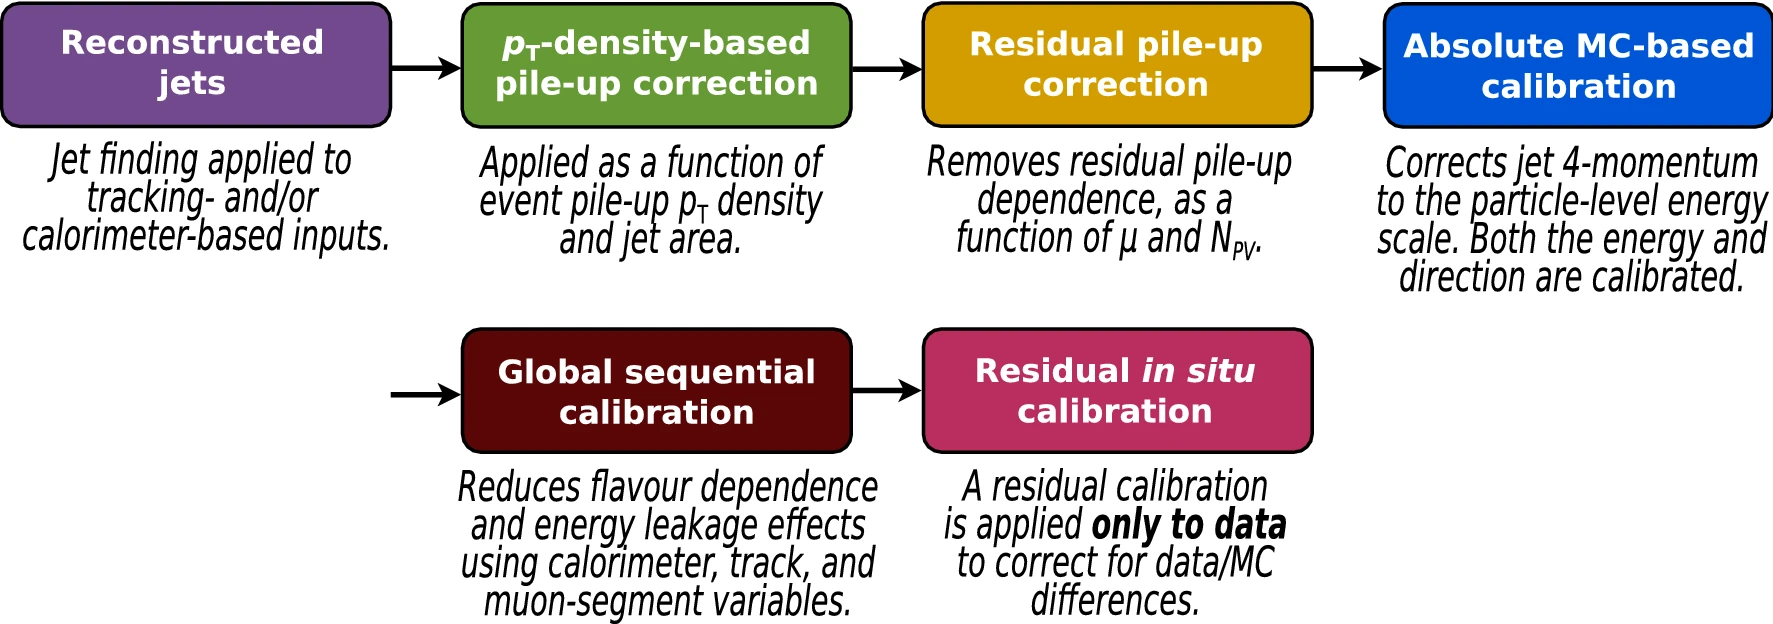
\includegraphics[width=\linewidth]{3_experiment/object_reconstruction/jet_calibration}
    \caption{\texttt{PFLow} 4-momemtum jet calibration steps~\cite{ATLAS-Jet-Calibration-Run2}.}
    \label{fig:objects:jets:jet_calib:jet_calib_sequence}
\end{figure}

To reduce the number of jets with a considerable fraction of energy coming from pile-up, the \ac{JVT} algorithm is used. This algorithm \fixme{update to NNJVT} reconstructs a multivariate discriminant that combines, among other quantities, the \ac{JVF} (fraction of the tracks' \pt associated to a jet originating from the \ac{PV}, and the total number of tracks) and the number of \acp{PV} in the event \Npv. As the jets that do not originate from the hard-scatter interaction are generally softer, the \ac{JVT} cut is applied only to jets with \(\pt<60~\gev\) and \(\abseta<2.4\). The default \ac{JVT} \ac{WP} is \(96\%\) efficient for hard-scatter jets.
















\section{Jet flavor tagging}

Heavy hadrons decays are governed mainly by the heaviest hadron in the decay cascade. A \(b\)-hadron generally decays through a cascade to a \(c\)-hadron, which in turn decays to an \(s\)-hadron, etc, which leads to the existence of multiple vertices.

\ac{FTAG} is the classification of jets containing \(b\)-hadrons (\bjets), \(c\)-hadrons (\cjets) or neither \(b\)-
or c-hadrons (light-flavour jets, or \ljets) by using algorithms sensitive to the distinctive properties of the respective classes.
These complex algorithms rely on the multiple vertices, on the high mass, high decay multiplicity and characteristic decay modes of the \(b\)- and \(c\)-hadrons, as well as on the properties of heavy-quark fragmentation.


In \ac{ATLAS} a two-step approach is employed to reconstruct key characteristics of heavy-flavour jets. In the first stage, low-level algorithms use complementary methods to extract track information from the charged particles linked to the jet. Some algorithms focus on the properties of individual tracks, while others analyse their correlations or combine them to explicitly reconstruct displaced vertices. In the second stage, the outputs from these algorithms are integrated into a high-level algorithm using multivariate classifiers to optimize performance. Over time, the algorithms have evolved significantly, starting with likelihood-based discriminants and boosted decision trees during \ac{LHC} Run-1, and progressing to more advanced methods like recurrent and deep neural networks, resulting in notable improvements on the identification performance~\cite{ATLAS-FTAG-Calibration-2012,ATLAS-FTAG-Efficiency-2012,MV2Algorithm,ATLAS-FTAG-DeepLearning}.

Starting in Run-3, a novel Transformer-based "GN2" algorithm is developed by the \ac{FTAG} combined performance group in \ac{ATLAS}. The GN2 algorithm is a single trained model which supersedes DL1d~\cite{ATLAS-FTAG-DL1-Run2} and the low level algorithms that feed it. It is based on GN1~\cite{ATLAS-FTAG-GN1}, and was quickly refied into GN2. GN2 replaces the Graph Attention Network~\cite{GANs} used by GN1 with a Transformer~\cite{GN2Transformer}, and also benefits from several other architectural optimisations and from an order of magnitude more training statistics.

GN2 directly accepts information about the jet and associated tracks and as such does not depend on other flavour tagging algorithms. GN2 retains the two the auxiliary training objectives that were introduced with GN1: the grouping of tracks originating from a common vertex, and the prediction of the underlying physics process from which each track originated.

This new algorithm is also prepared to provide identification of \cjets and jets originating from \(\tau\) decays. Outputs of this tagger comprise the probabilities of a jet to be tagged as a \(b\)-, \(c\)-, \(\tau\)- and light-flavor jet, labeled as \(p_b\), \(p_c\), \(p_{\tau}\) and \(p_u\), respectively.

\subsection{\bjet identification performance}

In order to evaluate the performance of the tagger of identifying \bjets at a constant efficiency, the ability to reject \(c\)-, \(\tau\)- and light-flavor jets is measured. The tagger output probabilities are combined to build a single discriminant \gntb, defined as
\begin{equation}
    \gntb = \log \left(
        \frac{p_b}{f_c p_c + f_{\tau} p_{\tau} + \left(1-f_c-f_{\tau}p_u\right)}
    \right).
\end{equation}
The parameters \(f_{c(\tau)}\) are free and determine the weighting between \(p_{c(\tau)}\) and \(p_u\) in the discriminant. The specific values of these parameters are determined through an optimisation procedure aimed at maximimsing the rejection of \cjets (\(\tau\)-jets) and \ljets and found to be \(0.2\) (\(0.01\)).


From the tagger discriminant score, several \acp{WP} can be defined, simply by requiring the \gntb score to by above a certain threshold. The \ac{FTAG} working group provides centrally to the whole \ac{ATLAS} collaboration 5 different \acp{WP} to achieve a fixed overall \btagging efficiency: \(65, 70, 77, 85\) and \(90\%\) efficiency, and are shown in \Fig{\ref{fig:objects:jet_tagging:btag_discrminant}}. In said figure, the data and \ac{MC} GN2 tagger distributions are compared, where the different flavour contributions are shown with different colors.

\begin{figure}[ht!]
    \centering
    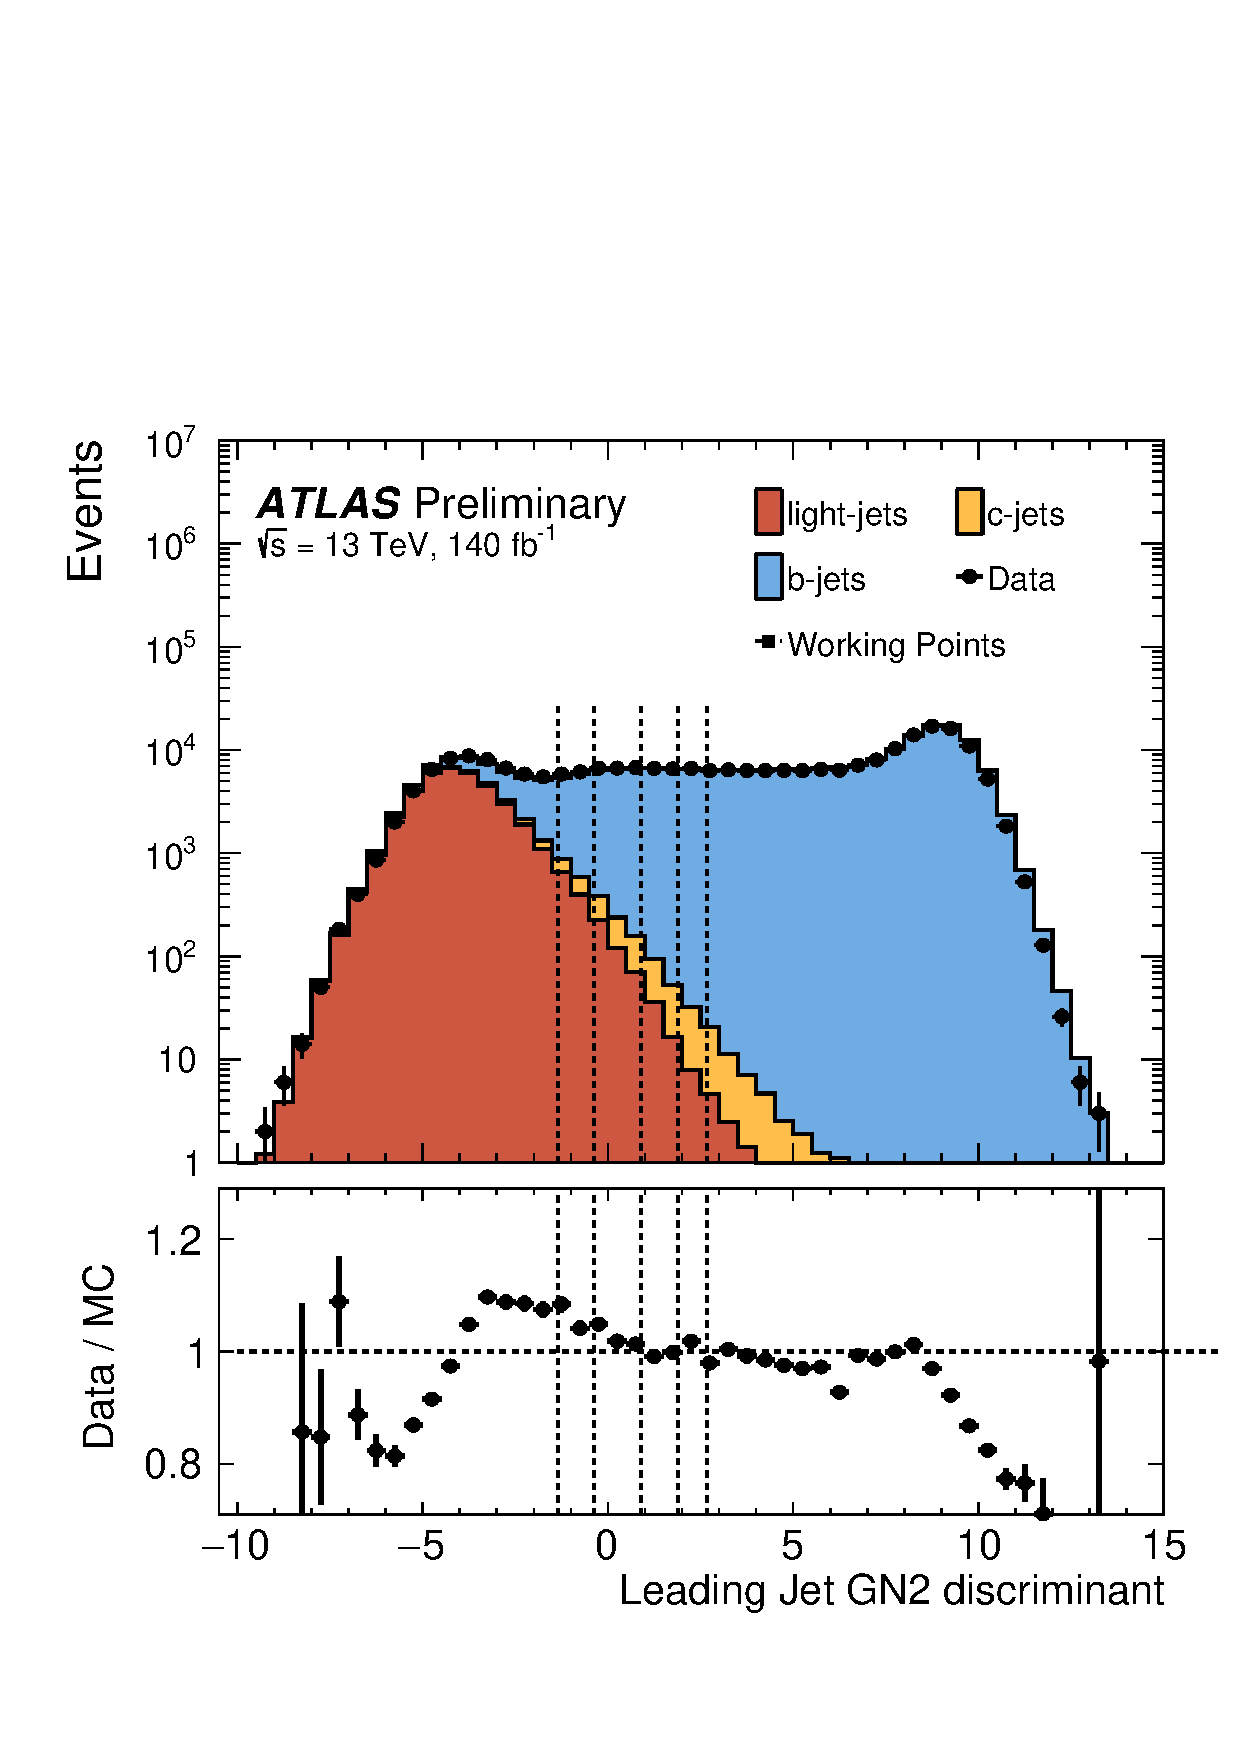
\includegraphics[width=0.6\linewidth]{3_experiment/object_reconstruction/btagging_discriminant}
    \caption{GN2 tagger discriminant comparison between data and single-lepton \ttbar \ac{MC} simulation. The \(l\)-, \(b\)- and \cjets are contributions are shown with different colors, and the 5 \btag \acp{WP} shown with the dashed vertical lines. From left to right, the dashed lines represent the \(90, 85, 77, 70\) and \(65\%\) efficiency \acp{WP}. The lower pad shows the ratio between data and the stacked \ac{MC}~\cite{ATLAS-FTAG-GN2BtagWPs}.}
    \label{fig:objects:jet_tagging:btag_discrminant}
\end{figure}

One key challenge of \btagging is the decrease in efficiency at higher \pt. In this high-\pt regime, particles become more collimated and they tend to travel further in the \ac{ID} before decaying, potentially leading to a decay track with spurious hits. The degraded efficiency is visualised in \Tab{\ref{tab:objects:ftag:btag_efficiency_original}}, where tagging efficiencies are shown for \bjets, along with \cjets, \ljets and \tjets rejections, in the low and high-\pt regimes. The values shown are computed by using different samples, where \ttbar is used at low-\pt and \(Z'\) decay events~\footnote{The leptophobic axial-vector \(Z'\) model is a simplified Dark-Matter model in which one of the theorised decay products are a pair of quarks.} are used in the high-\pt region. It can be seen that the \btag efficiency drops by \(30\%\) for higher \pt jets.

\begin{table}[ht!]
    \caption{Measured \btagging efficiencies and \cjets, \ljets and \tjets rejections in the low and high-\pt regime.}
    \label{tab:objects:ftag:btag_efficiency_original}
    \begin{tabular}{llcccc}
    \toprule
    Sample & \pt range [\gev]                                    & $b$-efficiency & $c$-rejection & light-flavor rejection & $\tau$-rejection \\ \midrule
    $t\bar{t}$  & \(20<\pt<250\)    & $0.76$         & $17.52$       & $448.61$               & $71.15$          \\
    $Z'$        & \(250<\pt<6000\)  & $0.41$         & $20.27$       & $179.99$               & $452.94$         \\ \bottomrule
    \end{tabular}
\end{table}

\subsection{\cjet identification performance}

Similar to \btagging, a single discriminant can be built from the output probabilities of the tagger in order to identify \cjets against \bjets, \(\tau\)-jets and \ljets:
\begin{equation}
    \gntc = \log \left(
        \frac{p_c}{f_b p_b + f_{\tau} p_{\tau} + \left(1-f_b-f_{\tau}p_u\right)}
    \right)
\end{equation}
where now the \(f_{b(\tau)}\) are the free parameters that control the rejection between \(b\)-, \(\tau\)- and light-flavor jets. Using the same optimisation procedure as for \btagging, the values for \(f_{b(\tau)}\) are found to be \(0.3\) (\(0.05\)).

Thanks to the great \btagging efficiency achieved by GN2, it is possible to design a \ctagging \ac{WP} after applying \btagging-veto, further separating \cjets from \ljets. By building this simultaneous tagging \ac{WP} and assuming the fraction of \tjets to be negligible, one can separate light-, \(c\)- and \(\bjets\) in three orthogonal regions. Starting from requiring a jet to \textit{not} pass the \(77\%\) \btagging \ac{WP} (\btag veto), three different \ctagging \acp{WP} are defined by fixing the \gntc score: \(10, \, 30\) and \(50\%\) \ctag efficiency. The efficiency and rejection measurements for the both samples described above, after applying the \(50\%\) \ctag \ac{WP} are shown in \Tab{\ref{tab:objects:ftag:ctag_efficiency_original}}.

\begin{table}[ht!]
    \caption{Measured \ctagging efficiencies and \bjets, \ljets and \tjets rejections in the low and high-\pt regime. The values shown correspond to those after applying the \btagging \(77\%\) \ac{WP} veto and the \(50\%\) \ctagging \ac{WP}. \fixme{rejection values not correct!}}
    \label{tab:objects:ftag:ctag_efficiency_original}
    \begin{tabular}{llcccc}
    \toprule
    Sample & \pt range [\gev]                                    & $c$-efficiency & $b$-rejection & light-flavor rejection & $\tau$-rejection \\ \midrule
    $t\bar{t}$  & \(20<\pt<250\)    & $0.467$         & $17.52$       & $448.61$               & $71.15$          \\
    $Z'$        & \(250<\pt<6000\)  & $0.344$         & $20.27$       & $179.99$               & $452.94$         \\ \bottomrule
    \end{tabular}
\end{table}


\fixme{Add plots with GN2 distributions?}












% \subsection{Monte Carlo generators}

% \paragraph{Sherpa}
% One of the general purpose event generators used in this thesis is \texttt{SHERPA} \cite{Sherpa}.  It includes matrix element generators as well as a built-in parton showering.  In this thesis,  simulated events with \texttt{SHERPA} include Multi-boson processes as well as the associate production of vector bosons and jets.  

% \paragraph{Powheg} 
% The \texttt{POWHEG} \cite{Powheg} framework is a matrix element generator at next-to-leading perturbative order.  The matrix element generation is interfaced with generators like \texttt{PYTHIA} or \texttt{HERWIG++} in order to simulate the parton shower.  This kind of combination of matrix element generator and parton shower simulation is used or top-related processes such as top-antitop pair production. 

% \paragraph{MadGraph5\_ aMC@NLO} \texttt{MadGraph5} \cite{Madgraph} is used as a matrix element calculator at next-to-leading perturbative order.  Similar to \texttt{POWHEG},  it is interfaced with \texttt{PYTHIA} or \texttt{HERWIG} to include parton showering. 

% \paragraph{Pythia}
% A second general purpose event generator used in this thesis is \texttt{PYTHIA 8}\cite{pythia},  even with matrix element calculation and parton showering possible within \texttt{PYTHIA}, it is widely used for its parton showering,  interfaced with \texttt{POWHEG} or \texttt{HERWIG}.  Additionally,  \texttt{PYTHIA} is used in this thesis to simulate minimum-bias proton-proton collisions.

% \paragraph{Herwig} The \texttt{HERWIG} \cite{Herwig,Herwig++} Monte Carlo event generator has capabilities to be used to simulate the matrix element,  but is only used within this thesis as a variation of the \texttt{PYTHIA} parton showering. 

% \paragraph{EvtGen}
% \texttt{EvtGen} \cite{EvtGen} is a framework that simulates the decay of final state particles.  Events associated with the production and decay of a top quark used in this thesis are simulated through a combination of \texttt{POWHEG}, \texttt{PYTHIA} and \texttt{EvtGen}.  Within this thesis, all events generated with a parton showering by \texttt{PYTHIA} include final state particle decays simulated with \texttt{EvtGen}.

% \subsection{ATLAS detector simulation}
% \label{sec:DAQ:AF2}


% To directly compare the data collected with the ATLAS detector with the prediction of \ac{SM} and \ac{BSM} events in simulation,  the interaction of the produced particles with the detector material has to be simulated.
% The Geant4 \cite{Geant4} software package is used to simulate the interaction of particles with the detector material.
% A full Geant4 model of the ATLAS detector is used to simulate the transition of particles produced in proton-proton collisions through the different detector layers. 

% The simulation of a large number of interactions necessary to mimick the ATLAS reconstruction is computationally extensive.  Especially the simulation of shower developments in the calorimeters consumes a large amount of CPU and computing time. 
% For many \ac{BSM} searches,  a large number of parameters affecting the predicted particle masses and interactions have to be simulated.  A 'fast' parameterised detector simulation has been developed to cope with this high simulation demand.  A so-called Atlfast-II or AFII setup simulation chain uses Geant4 simulation for the interactions in the \ac{ID} and muon spectrometer,  but a parametrised simulation called FastCaloSim for the particle interactions in the electromagnetic and hadronic calorimeter. 
% The improvements in computing time compared to Geant4 simulation of the full detector as well as a fast,  simplified Geant4 simulation is shown in Figure \ref{fig:DAQ:AFIIvsG4}.  The overall processing time is reduces by roughly an order of magnitude compared to the full Geant4 simulation \cite{AFIIprinciple}. 
% \begin{figure}[h]
% \centering
% \includegraphics[width=0.8\linewidth]{figures/DAQ/AFII_CPU_improvement.png}
% \caption{CPU time distributions for 250 $ \ttbar $ events compared for G4,  fast G4 and AFII setup,  taken from \cite{AFIIprinciple} \label{fig:DAQ:AFIIvsG4}}
% \end{figure}
% The fast calorimeter simulation FastCaloSim uses a parametrisation of the calorimeter response.  The parametrisation has been extracted through Geant4 simulation and tunes to data. 
% The main three simplifications include simplifying the detector geometry,  approximating the calorimeter cells as cuboids,  only reproducing the average lateral energy distributions and restricting the simulation to three types of initial particles. 




\FloatBarrier
\part{Photon shower shape corrections}
\label{part:pid}
\chapter{Photon identification and shower shapes}
\label{ch:pid_ss}
\epigraph{\emph{“Champions keep playing until they get it right.”}}{Billie Jean King}

% In \Sect{\ref{subsec:objects:egamma:id}} a very brief description on the identification procedure was described. In the current chapter, a more detailed explanation on the process as well as on the variables used to perform the photon identification is presented. \fixme{elaborate more}

The \ac{ECAL} was presented briefly in \Sect{\ref{subsubsec:atlas:atlas:cals:ecal}}, where the measurement mechanism and all the layers it has was described. In this subdetector, photons deposit their energy via electron-positron pair creation and bremsstrahlung radiation, creating an \ac{EM} shower. The \ac{ECAL} does a great job to compute the energy of the \ac{EM} shower, but identifying the initiating particle remains a challenging task. 
However, by virtue of the different layers and granularities in the \ac{ECAL}, different characteristics of these \ac{EM} showers can be studied, and are encoded by different variables called \acfp{SSV}.

% \fixme{give the overview of the chapter?} As a first step, the variables used to identify correctly the photons are described in detail and the current problem of disagreement between data and \ac{MC} is explained. 






\section{Shower shapes}
\label{sec:pid_ss:ss}

As mentioned in \Sect{\ref{subsec:objects:egamma:id}}, photon identification relies on rectangular cuts applied to \acp{SSV} that lead to an excellent separation power between real isolated photons from fake photons originating from hadrons. These \acp{SSV} are computed from the photon candidates' energy deposits in the \ac{ECAL} and \ac{HCAL} cells, and serve to describe the passage of the photons candidates throughout the calorimeters, characterizing the lateral and longitudinal \ac{EM} showers.

In general, real photons produce narrower energy deposits in the \ac{ECAL}, and have lower leakages to the \ac{HCAL}, compared to those photons proveninent from hadrons, where the presence of additional neighbouring hadrons close to the fake photon tend to widen the showers. Furthermore, since the first layer of the \ac{ECAL} consists on fine strips, it is possible to discriminate photon candidates coming from \(\pizero\to\gamma\gamma\) decays, characterized by two local maxima due to the presence of two nearby photons.

\begin{table}[ht!]
    \caption{Discriminative \acp{SSV} used for photon identification. The three columns on the right denote whether the variable is used for the \textit{loose} (L), \textit{medium} (L) or \textit{tight} (T) identification \ac{WP} or not.}
    \centering
    \resizebox{\textwidth}{!}{
        \begin{tabular}{p{.2\textwidth}p{.50\textwidth}p{0.12\textwidth}|p{.01\textwidth}p{.01\textwidth}p{.01\textwidth}}
            \hline
            \hline
            Category  &  Description  &  Name & L & M & T \\
            \hline
            \hline
            Hadronic leakage
            &  Ratio of \et in the first sampling layer of the \ac{HCAL} to \et of the \ac{EM} cluster (used over the ranges \(\abseta<0.8\) and \(\abseta>1.52\))
            &  \(R_{\text{had 1}}\)  & \checkmark & \checkmark & \checkmark\\
            &  Ratio of \et in the \ac{HCAL} to \et of the \ac{EM} cluster (used over the range \(0.8<\abseta<1.37\))
            &  \(R_{\text{had}}\) & \checkmark & \checkmark & \checkmark\\
            \hline
            EM second layer
            &  Ratio of the energy in \(3\times 7\) \(\eta \times \phi\) cells over the energy in \(7 \times 7\) cells centered around the photon cluster position
            &  \(R_{\eta}\) & \checkmark & \checkmark & \checkmark\\
            &  Lateral shower width in \(\eta\) & \(w_{\eta 2}\)  & \checkmark & \checkmark & \checkmark\\
            &  Ratio of the energy in \(3 \times 3\) \(\eta \times \phi\) cells over the energy of \(3 \times 7\) cells centered around the photon cluster position
            &  \(R_{\phi}\) &  & \checkmark & \checkmark\\
            \hline
            EM first layer      
            &  Lateral shower width in 3 strips around the maximum
            &  \(w_{\eta 1}\) or \(w_1\) &  & \checkmark & \checkmark\\
            &  Total lateral width
            &  \(w_{\text{s tot}}\) &  & \checkmark & \checkmark\\
            &  Energy outside the core of the three central cells, within seven cells divided by the energy within the three central strips &  \(f_{\text{side}}\)  &  & \checkmark & \checkmark\\
            &  Difference between the energy associated with the second maximum in the strip layer with the minimum value found between the first and second maxima.
            &  \(\Delta E\)  &  & \checkmark & \checkmark\\
            &  Ratio of the energy difference between the maximum energy deposit and the energy deposit in the secondary maximum in the cluster to the sum of these energies
            &  \(E_{\text{ratio}}\)  &  & \checkmark & \checkmark\\
            &  Ratio of the energy in the first layer to the total energy of the \ac{EM} cluster
            &  \(f_1\) & & \checkmark & \checkmark\\
            \hline
            \hline
        \end{tabular}
    }
    \label{tab:pid_ss:ss:ss_variables}
\end{table}

In the following, the \acp{SSV} used for photon identification are detailed, and shown summarised in \Tab{\ref{tab:pid_ss:ss:ss_variables}}.
The first variable makes use of the energy measured in the \ac{HCAL}:
\begin{itemize}
    \item Hadronic leakage: is the trasnverse energy deposited in the \ac{HCAL}, normalized to the energy deposited in the \ac{ECAL}:
        \begin{equation}
            {\rhad}_{(1)} = \frac{\et^{\text{had}}}{\et^{\text{EM}}}
        \end{equation}
        In order to minimize the effects of resolution degradation, in the barrel-endcap transition region of the \ac{HCAL} (\(0.8\leq \abseta\leq 1.37\)) the energy deposit in the whole \ac{HCAL} is used (\rhad). On the reminaing of the detector, only the energy deposited in first layer of the \ac{HCAL} is used (\rhado).
\end{itemize}
The following variables use the second-layer information of the \ac{ECAL}:
\begin{itemize}
    \item Lateral energy profile in \(\eta\):
        \begin{equation}
            \reta = \frac{E_{3\times7}^{s2}}{E_{7\times7}^{s2}}
        \end{equation}
        where \(E_{i\times j}^{s2}\) is the energy sum in the second calorimeter layer contained in a window of \(i \times j \) cells (units of \(\eta \times \phi\) cells), centered at the most energetic cell. This variable gives a measure of the showers' width in the \(\eta\) direction.
    \item Lateral energy profile in \(\phi\):
        \begin{equation}
            \rphi = \frac{E_{3\times3}^{s2}}{E_{3\times7}^{s2}}
        \end{equation}
        defined in a similar way as \reta. However, this variable behaves very different for converted and unconverted photons. Due to the action of the magnetic field, the electrons and positros are curved into opposite directions in \(\phi\), having as a result, \ac{EM} showers much wider in the case of converted photons than those for unconverted ones.
    \item Lateral shower width in \(\eta\):
        \begin{equation}
            \weta = \sqrt{
                \frac{\sum E_i \eta_i^2}{\sum E_i}
                -
                \left(\frac{\sum E_i \eta_i}{\sum E_i}\right)^2
            }
        \end{equation}
        measures the proper width of the \ac{EM} shower, where \(E_i\) is the energy in the \(i\)-th cell of the \ac{ECAL}, measured in a window of \(3\times 5 \) cells in \(\eta \times \phi\).
\end{itemize}
The following variables use the information from the first \ac{ECAL} layer, composed of the strip cells that allow for a high \(\eta\) resolution and allows for a good separation between isolated photons from photons product of the \(\pizero\) decay. \Fig{\ref{fig:pid_ss:ss:pizero}} shows the difference in the energy deposited in the \ac{ECAL} between the two cases mentioned previously.
\begin{itemize}
    \item Lateral energy profile in \(\eta\)
        \begin{equation}
            \fside = \frac{E_7^{s1} - E_3^{s1}}{E_3^{s1}}
        \end{equation}
        measures the energy outside the core of the three central strips within a window of 7 cells, divided by the energy in the three central cells.
    \item Lateral shower width in \(\eta\) (3 strips)
        \begin{equation}
            \wone = \sqrt{
                \frac{\sum E_i (i - i_{max})^2}{\sum E_i}
            }
        \end{equation}
        where \(i\)runs over all cells in a window of 3 cells around the highest-energy-cell. This variable measures the width of the \ac{EM} shower in the first layer of the calorimeter.
    \item Lateral shower width in \(\eta\) (full).
        It is defined in a similar way as \wone, but uses all the cells in a window of \(\delta\eta\times\delta\phi=0.0625\times 0.2\), corresponding to approximately to \(20\times 2\) strips \(\eta\times\phi\).
    \item Energy difference
        \begin{equation}
            \deltae = E_{\text{max}, 2}^{s1} - E_{\text{min}}^{s1}
        \end{equation}
        represents the energy difference between the second maximum and the minimum reconstructed energy between the two maxima in the strip layer.
    \item Energy ratio
        \begin{equation}
            \eratio = \frac{
                E_{\text{max}, 1}^{s1} - E_{\text{max}, 2}^{s1}
            }{
                E_{\text{max}, 1}^{s1} + E_{\text{max}, 2}^{s1}
            }
        \end{equation}
        is the ratio of energy difference between the two maxima, normalized to the sum of those energies, in the strip layer.
\end{itemize}

\begin{figure}[ht!]
    \centering
    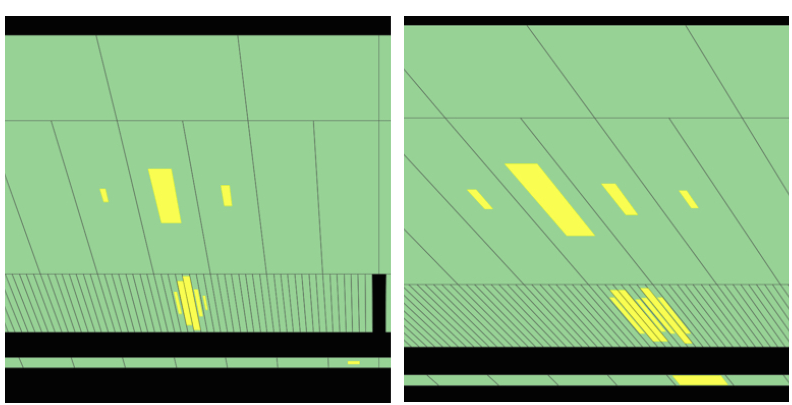
\includegraphics[width=0.7\linewidth]{4_photonid/shower_shapes/PhotonPizero}
    \caption{Characteristic energy deposits by an isolated photon (left), and a \(\pizero\to\gamma\gamma\) event (right), which is possible to distinguish thanks to the granularity of the first \ac{ECAL} layer~\cite{ATLAS-ECAL-Pizero}.}
    \label{fig:pid_ss:ss:pizero}
\end{figure}






\section{Photon Identification}


\subsection{Optimisation}
\label{subsec:pid_ss:pid:optimisation}

Starting from these discriminating \acp{SSV}, three \acp{WP} can be defined: \textit{loose}, \textit{medium} and \textit{tight} \acp{WP}~\cite{ATLAS-EGamma-Performance-2024}. The loose \ac{WP} is employs cuts to the variables defined in the second layer and to the hadronic leakage variable, used primarily by the trigger. The medimum \ac{WP} is a \ac{WP} optimised to have a flat \(95\%\) efficiency. This \ac{WP} applies cut to all the previously defined variables (strip and middle layer and leaks to the \ac{HCAL}). Finally, the tight \ac{WP}, uses all the \acp{SSV} defined and provides an excellent background rejection. TABLE shows which variables are used for each \ac{WP}.

ADD PLOTS OF ALL THE VARIABLES COMPARING REAL AND FAKE

The cuts on the \acp{SSV} for each identification \ac{WP} are optimised as a function of the transverse energy and the pseudo-rapidity of the photon candidate, to account for the shape of the variables for different \(\eta\) and for variations in the amount of material and the geometry of the calorimeter. The three \acp{WP} are also optimised separately for converted and unconverted photons.
The optimisation is performed with a \ac{MV} approach where signal efficiencies are scanned between \(0\%\) and \(100\%\) while trying to maximise the background rejection. The resulting, optimised, cut values are subject to fluctuations and therefore they are manually smoothed.

Two different \ac{MC} samples are used for the optimisation procedure, representative at different \ptgam. For photons with \(10<\pt<25~\gev\), radiative \Zboson decays (\(\Zboson\to\ellell\gamma\)) samples are used as signal, while \Zjets events accounts for the background. Events used are selected by requiring two opposite charged leptons and a minimum angular separation between the photon and the lepton of \(\DeltaR_{\text{min}}(\ell, \gamma) > 0.4\). To reject non-radiating \Zboson bosons, the dilepton invariant mass has to satisfy \(m_{\ell\ell}<83~\gev\), and the three-body invariant mass \(m_{\gamma\ell\ell}\) needs to approximate the \Zboson boson mass: \(80~\gev < m_{\gamma\ell\ell} < 100~\gev\). Finally, the photon is required to have \(\abseta<2.37\), excluding the crack region.
Finally, for higher \pt photons, \(\pt>25~\gev\), the inclusive-photon (\yj) signal events are compared agains dijet backgrounds. The event selection used in this case is simply requiring the photon to be in the \ac{ECAL} acceptance region (excluding the crack).





\subsection{Efficiency measurements}

Photon identification efficiency measurements are carried out using three different methods that are detailed in \Refn{\cite{ATLAS-EGamma-Performance-2015-2016}} and that are combined to yield correction factors for analyses. In all cases, photons are required to satisfy the Loose isolation criterion defined in \Refn{\cite{ATLAS-EGamma-Performance-2015-2016}} and therefore the photon efficiencies are measured relative to this isolation criterion. In the following paragraphs, a brief description of each method is given.

For the lower \pt range (\(7<\pt<100~\gev\)), photons from radiative \Zboson decays are used as signal photons, selecting the events in the same way as for the \acp{WP} optimisation (\Sect{\ref{subsec:pid_ss:pid:optimisation}}). The only difference in this case, is an additional lower limit on the di-lepton invariant mass of \(40<m_{\ellell} < 83~\gev\). To estimate the number of signal and background events, template fits to the observed three-body invariant-mass distribution are performed.

The second method to compute efficiencies relies on Smirnov transformations~\cite{SmirnovTransform} to the electrons' \acp{SS} to resemble those of photons'. The samples used in this approach are \(\Zboson\to ee\) decays, in which the electrons are required to pass loose photon isolation. The candidate electrons in data contain a small background from \Wjets and multijet production; this background is subtracted by fitting simulated signal samples and background templates derived from data control regions to the \(m_{ee}\) data distributions. The electron candidates are counted for events in the range \(70 < m_{ee} < 110~\gev\), and the efficiencies are measured using the tag-and-probe method described in \Refn{\cite{ATLAS-EGamma-Performance-2015-2017}}. The \pt range in which this method is implemented is \(25<\pt<250~\gev\).

The final and third method uses higher \pt photons originating from \ac{QCD} \gammajet production with transverse momenta in the range \(50<\pt<1500~\gev\). The photons for this study are required to pass the loose identification \ac{WP} employed in the trigger. This sample is dominated by background dijet events whose production cross section is orders of magnitude higher. The maxtrix method~\cite{ATLAS-EGamma-Performance-2015-2016} is used in this case, which constructs four orthogonal regions that either pass or fail the tight identification \ac{WP}, and pass or fail the track-isolation (described in \Sect{\ref{subsec:objects:egamma:iso}}). For each region, two unknowns arise: the number of signal and background events.
If the track isolation efficiencies are known for the signal and background components, then it is possible to estimate the efficiency for loose photons passing the tight identification criteria. The isolation efficiencies for signal photons are estimated using \ac{MC} samples, and the ones for backgrounds are obtained in a jet-enriched control region constructed by inverting the identification criteria.
The efficiency measurements in data for the tight identification \ac{WP} then reads:
\begin{equation}
    \varepsilon^{\text{tight-ID}} = \frac{
        \frac{
            \hat{\varepsilon}_{\text{ID}} - \hat{\varepsilon}_{\text{ID}}^b
        }{
            \hat{\varepsilon}_{\text{ID}}^s - \hat{\varepsilon}_{\text{ID}}^b
        }
        \cdot
        N_{\text{ID}}^T
    }{
        \frac{
            \hat{\varepsilon} - \hat{\varepsilon}^b
        }{
            \hat{\varepsilon}^s - \hat{\varepsilon}^b
        }
        \cdot
        N^T
    },
\end{equation}
where \(N^T\) accounts for the totality of photons in the inclusive sample which consists on \(N^s\) prompt photons (or signal photons) and \(N^b\) fake photons (background photons). The number \(N^T_{\text{ID}}\) is the subset of \(N^T\) that pass the identification requirement. Data, signal and background track isolation efficiencies are represented by \(\hat{\varepsilon}\), \(\hat{\varepsilon}^s\) and \(\hat{\varepsilon}^b\), respectively. Similarly, the track isolation efficiencies for those photons passing tight identification are shown as \(\hat{\varepsilon}_{\text{ID}}\), \(\hat{\varepsilon}_{\text{ID}}^s\) and \(\hat{\varepsilon}_{\text{ID}}^b\), respectively. The measured efficiencies for photons with \(\pt>150~\gev\) is between \(90\) and \(96\%\).

Since data and simulation measured efficiencies do not match, \ac{MC} needs to be corrected to account for these differences. In the ideal case where one expects perfect agreement between both samples, ratios of the data efficiencies to simulation efficiencies in each \(\pt-\eta\)-conversion status bin should be \(1.0\). These ratios are referred as \acp{SF} and are computed separately for each one of the methods described. Then, the different methods' \acp{SF} are combined using a weighted average in each bin, assuming the statistical and systematic uncertinaties to be uncorrelated between the methods. Resulting \acp{SF} in all cases are consistent with \(1.0\), only deviating by a maximum of \(2\%\). The only exception to this case is in the first \pt-bin (\(7<\pt<10~\gev\)) where deviations of up to \(30\%\) take place.





\section{Shower shapes variables differences between data and MC}

The \ac{ATLAS} \ac{MC} simulation does not perfectly describes data. This is clearly seen when computing the previsously mentioned \acp{SF}, whose values were different from 1, meaning that different efficiencies are obtained in data and in \ac{MC}. In particular, when comparing the \acp{SS} distributions, it is seen that \ac{MC} distributions are shifted or even the whole shape differs.

The main differences on the distributions arise for the \(\eta\) shower profiles, where broader distributions were seen in data compared to \ac{MC}. Part of the effect was corrected in 2010 after moving to detailed description of the material composition in the accordion absorbers in \textsc{Geant4}. However, the remaining data-\ac{MC} disagreements are still under study and could be due to several potential effects:
\begin{itemize}
    \item Detector geometry description of the lead thickness (including possible variations of due to gravity) or material composition, material before the \ac{ECAL}, a decrease of the width of cells caused by calorimeter contraction due to temperature (mainly in the first layer).
    \item Mismodeling of the electric field in the \ac{LAr} gaps.
    \item Mismodeling of the cross-talk effect (energy sharing between calorimeter cells due to electronics possible in \(\eta\) direction).
\end{itemize}



To account for the differences in the \acp{SS}, historically, corrections were made in the form of shifts to each one of the \ac{MC} distributions. These shifts comprised the so-called \acp{FF}, and were determined using a \chisq minimisation on the comparison of data and \ac{MC} \acp{SS}~\cite{ATLAS-EGamma-Performance-2015-2016,ATLAS-EGamma-Performance-2015-2017}.
Even though the differences decreased substantially after these corrections, some of them remained, shown in FIGURE. It is seen from the distributions that the main differences that remained are related to the shape of the distributions, therefore needing for higher order corrections. In \Ch{\ref{ch:ffs}} a detailed description of newly derived corrections is presented.
Since \acp{SS} are built from energy deposits on the \ac{ECAL} cells, another possible way of correcting the current disagreement between data and \ac{MC} \acp{SS} is to directly correct the energies on \ac{MC} at a cell-level, fixing the differences in all \acp{SSV} at once. This new approach is studied in \Ch{\ref{ch:cellrw}}.


\section{Samples and event selection for the \ac{SS} correction studies}

As mentioned above, the improved \ac{FF} method and a novel cell-based reweighting method is presented in \Chs{\ref{ch:ffs}}{\ref{ch:cellrw}}.

Similar to what had been done for the identification optimisation studies, two photon samples are used for the \acp{FF} calculation. For photons with \(7\leq\ptgam\leq 50~\gev\), \ac{FSR} photons from \Zboson-boson decay are considered, while photons from \ac{QCD} \gammajet events are used for photons with \(\ptgam\geq50~\gev\), hereinafter referred as \ac{RZ} photons and \ac{SP} samples, respectively. On the other hand, for the cell-level corrections to the \acp{SSV}, only \ac{RZ} photons are used. In what follows, event selection for both types of samples is detailed.

For both types of corrections, the \ac{MC} samples are reweighted to match the luminosity of the collected \ac{ATLAS} data, and also pileup re-weighted to match the pileup profile shown in \Sect{\ref{sec:atlas:runs}}.

\subsection{Radiative \Zboson boson decays}

For low-\pt photons, \ac{RZ} photons are used as signal photons, while backgrounds are modeled by \(\Zboson\to\ell\ell\) events. The photons are required to pass the following selection:
\begin{itemize}
    \item \textbf{\ac{ECAL} \abseta acceptance region}. First of all, the photons are required to be inside the \ac{ECAL} acceptance region excluding the crack, detailed in \Sect{\ref{subsubsec:atlas:atlas:cals:ecal}}, given by \(\abseta<1.37\) or \(1.52<\abseta<2.37\). 
    \item \textbf{Isolation}. Fake photon candidates are removed by imposing an isolation requirement on the calorimetric isolation variable with the \texttt{FixedCutTightCaloOnly} \ac{WP}.
    \item \textbf{\ac{FSR} selection}. As shown in FIGURE, the vast majority of events correspond to \(m_{\gamma\ell\ell}>100~\gev\) and \(m_{\ell\ell}\sim m_{\Zboson} \approx 91~\gev\), which represent \ac{ISR} photons (photons radiated from the inital quarks). Photon candidates from \ac{ISR} are largely affected by the \Zjets background, where a jet fakes a photon~\footnote{The production cross-section of \Zjets is about three orders of magnitude higher than that of \(\Zboson+\gamma\), and a non-negligible fraction of jets contains high-\pt \pizero's, decaying to collimated photon pairs}.
    However, a second peak appears in the distribution where the three-body invariant mass approximates the \Zboson mass (\(m_{\gamma\ell\ell}\approx m_{\Zboson}\)). These particular type of events are referred as \ac{FSR} photons, characterised by high real photon purity, and are the ones of interest for the correction studies.
    \item \textbf{Photon-lepton overlap}. By requiring a minimum angular distance between the photon and the closest lepton (\(\DeltaR_{\text{min}}>0.4\)), biases in the \ac{ECAL} deposits by the objects are avoided.
    \item \textbf{Truth-matching}. \fixme{give description here}
\end{itemize}


\subsubsection{Special selection for cell-based reweighting corrections}

For the cell-energy reweighting method to correct the \acp{SS}, a special selection needs to be applied to the \ac{EM} clusters. For the current studies, only \acp{SS} built from the second layer are studied. Clusters of \(7\times 11\) cells in \(\eta\times\phi\) are considered, shown in FIGURE with the current cell arrangement used.

In this work, only "healthy clusters" are considered, that is, events need to be associated to clusters of 77 cells (no cells missing) and the central cell must be the one with highest energy in the corresponding cluster ("hottest" cell). In FIGURE, an example of the averaged energies at each cell, for events with unconverted photons in data is shown.

For these particular studies, the photon isolation requirement is relaxed to the \texttt{FixedCutLoose} \ac{WP} is used.

%  and no identification selection is applied. The same \ac{FSR} requirements are posed on the events in which the invariant masses must satisfy \(80 < m_{\gamma\ell\ell} < 100~\gev\) and \(40<m_{\ellell} < 83~\gev\) which removes the majority of non-\ac{FSR} photons. The photon to the closest lepton candidate are required to be separated by a minimum angular distance of \(\DeltaR_{\text{min}}>0.4\), and the photons need to be in the \ac{ECAL} acceptance region of 

\subsection{Inclusive photons}

Photon+jet events are used for the high-\pt regime of the \acp{FF} corrections. The events pass loose identification trigger requirements and for the nominal values of the corrections tight identification is applied. This selection is applied to reduce the vast di-jet background, which has much higher production cross-sections. As for the \ac{RZ} photon samples, the photons are required to be within the \ac{ECAL} acceptance region excluding the crack.
\chapter{Shower shapes corrections}
\label{ch:ss_corrections}
\epigraph{\emph{“Champions keep playing until they get it right.”}}{Billie Jean King}


In the previous chapter, it was seen that \acp{SF} (ratio of data efficiencies to simulated ones) deviate from unity. Given that photon identification relies on cuts to the photon \acp{SS}, it was found that the differences in fact appear on these variables. Since Run-1, they have been corrected with what is known as \acfp{FF}, which, historically, they have been computed as simple shifts to the \ac{MC} distributions and have been found to provide very good improvements on the \acp{SF}. However, as seen before, there are still discrepancies between the distributions that need to be addressed in order to rely on even a better simulation.
In \Sect{\ref{sec:ss_corrections:ffs}}, a more sophisticated approach based on a higher order computation to correct the \acp{SS} is presented. Also, a novel approach using directly the cells energies is studied and addressed in \Sect{\ref{sec:ss_corrections:cell_rw}}. The studies presented in this chapter comprise one of the main topics of work for the current thesis.





\section{\acfp{FF}}
\label{sec:ss_corrections:ffs}


\subsection{Data and simulated samples}
\label{subsec:ss_corrections:ffs:samples}

\acp{FF} are computed using full Run-2 dataset, collected at \(\sqrt{s}=13~\tev\) and with a corresponding integrated luminosity of \(140~\ifb\).
Both the \ac{RZ} and \ac{SP} simulated samples are used for this study, as their represent complementary \pt-ranges. \ac{RZ} events are generated with \SHERPA 2.2.11~\cite{Sherpa2.2}, while \SHERPA 2.2.1 is used for \(\Zboson \to \ell\ell\) background events. Respecting the \ac{SP} samples, events are generated with \PYTHIA 8.186~\cite{Pythia8.1}, which includes leading-order \gammajet events from both direct processes (\(qg\to q\gamma\) and \(\qqbar \to g \gamma\)) and photon fragmentation from \ac{QCD} dijet events.

In both cases, the \ac{ATLAS} detector is simulated using \GEANT 4~\cite{Geant4} and the \ac{MC} events are reweighted so that their pileup distributions resembles the one in data, for each year of the Run-2 data-taking period.


\subsection{Calculation}
\label{subsec:ss_corrections:ffs:calculation}

% \acp{FF} are computed in a series of steps that start by preparing the input datasets up to the systematic uncertainties calculation. In the first step, histograms of all the \acp{SSV} are created and then smoothed, which are then used to perform the actual optimisation of the \acp{FF}.
% % This process is repeated for different isolation and identification selection requirements, in order to compute the systematic uncertainties.
% In the following a step by step description of the process is described.

The calculation is performed separately for the two considered samples: \ac{RZ} for photons with \(7\leq\pt\leq 50~\gev\) and \ac{SP} for photons with \(\pt> 50~\gev\), which were already discussed in \Sect{\ref{subsec:pid_ss:pid:event_selection}}. Since \acp{SS} distributions vary as a function of \pt and \abseta, the computation is done in bins of these variables:
\begin{gather}
    \ptgam:
    \begin{cases}
        \text{\ac{RZ}}: [7,\, 15,\, 20,\, 30,\, 50] ~\gev\\
        \text{\ac{SP}}: (50,\, 60,\, 80,\, 100,\, 150,\, 300,\, 600,\, \infty] ~\gev\\
    \end{cases}\\
    \abseta: [0,\, 0.6,\, 0.8,\, 1.15,\, 1.37,\, 1.52,\, 1.81,\, 2.01,\, 2.37].
\end{gather}
Furthermore, as mentioned in \Sect{\ref{sec:pid_ss:ss}}, there are variables very sensitive to the photon's conversion status, that is, whether if the photons are converted or unconverted. For this reason, the calculation is done separately for converted and unconverted photons. A total of nine variables are corrected using this method: \eratio, \fside, \reta, \rphi, \rhad, \rhado, \wone, \weta and \wstot; as they are the ones in which the largest discrepancies are observed between data and \ac{MC}.

For each \ac{SS}, histograms of \ac{MC} and data of 100 bins are created. The choice of the binning is done based on having sufficient statistics at each bin and also to capture all the features of the variables.
After that, each histogram is smoothed using the \acf{KDE} tool from TMVA~\cite{TMVA}. The \ac{KDE} method consists of estimating the shape of a \acf{PDF2} by the sum over smeared events. The \ac{PDF2} \(p(x)\) of a variable \(x\) is
\begin{equation}
	p(x) = \frac{1}{N}\sum_{i=1}^{N} K_h(x-x_i)
\end{equation}
where \(N\) is the number of events, \(K_h(t) = K(t/h)/h\) is the kernel function, and \(h\) is the bandwidth of the kernel. The basic idea is that each event is considered as a Dirac-\(\delta\)-function, which is replaced by a Kernel function (Gaussian) and finally they are summed altogether to form the final \ac{PDF2}. The \ac{KDE} smoothing can be applied in two forms: non-adaptive \ac{KDE} or adaptive \ac{KDE}, as seen in \Fig{\ref{fig:ss_corrections:ffs:calculation:adaptive_nonadaptive_kde}}. In the former, the bandwidth is constant for the entire sample \(h_{NA}\), while in the latter, it uses the value from non-adaptive \ac{KDE}, but it varies as a function of \(p(x)\) as
\begin{equation}
	h_A = \frac{h_{NA}}{\sqrt{p(x)}}
\end{equation}
Adaptive \ac{KDE} improves the shape of the estimated \ac{PDF2} in regions of low statistics, however, in high statistics regions it can give rise to over-smoothing. The degree of smoothing is tuned by multiplying the bandwidth \(h\) by fine factors. 
These fine factors are user-defined parameter which are tuned to allow the \ac{PDF2} to retain the important features of the \ac{SS} but to also avoid statistical fluctuations. Higher values indicate broader Kernel functions and therefore de \ac{PDF2} catches less statistical fluctuations.
Examples of the smoothing procedure applied to \rhad are shown in \Fig{\ref{fig:ss_corrections:ffs:calculation:smoothing_ss}} for cases in which original histograms have low and high statistics.

\begin{figure}[ht!]
    \centering
    \includegraphics[width=0.6\linewidth]{4_photonid/ffs/smoothing/kde}
    \caption{Adaptive and non-adatptive \ac{KDE} smoothing.}
    \label{fig:ss_corrections:ffs:calculation:adaptive_nonadaptive_kde}
\end{figure}

\begin{figure}[ht!]
    \centering
    \begin{subfigure}[h]{0.49\linewidth}
        \centering
        \includegraphics[width=\linewidth]{4_photonid/ffs/smoothing/can__pdfhist__mc__ph_rhad1__c_pt15p0_eta1p15}
        \caption{Low statistics case: \ac{RZ}}
    \end{subfigure}
    \hfill
    \begin{subfigure}[h]{0.49\linewidth}
        \centering
        \includegraphics[width=\linewidth]{4_photonid/ffs/smoothing/can__pdfhist__mc__ph_rhad1__u_pt0060p0_eta1p15}
        \caption{High statistics case: \ac{SP}}
    \end{subfigure}
    \caption{\ac{KDE} smoothing applied to the \rhad for photons in \(0.8<\abseta<1.15\) in two scenarios: low and high statistics. Original histograms are shown with the blue points and their \acp{PDF2} with the orange lines. The fine factors used for each case are displayed in the figure.}
    \label{fig:ss_corrections:ffs:calculation:smoothing_ss}
\end{figure}


Once the data and \ac{MC} \acp{PDF2} are created for a given variable, \pt, \abseta and conversion type, the \ac{MC} \ac{PDF2} is normalised to data's and a \chisq value is computed between both, excluding the underflow and overflow bins, as:
\begin{equation}
	\chisq = \sum_{i=1}^{N} \dfrac{(w_{\text{MC},i} W_{\text{data}} - w_{\text{data},i} W_{\text{MC}})^2}{s_{\text{MC},i}^2 W_{\text{data}}^2 + s_{\text{data},i}^2 W_{\text{MC}}^2}.
\end{equation}
\(N\) is the number of bins in the \acp{PDF2}, \(w_{\text{MC},i}\) and \(w_{\text{data},i}\) are the event numbers of \ac{MC} and data at each bin, respectively, \(s_{\text{MC},i}\) and \(s_{\text{data},i}\) are the bin errors and finally \(W_{\text{data}}\) and \(W_{\text{MC}}\) are the sum of weights for data and \ac{MC}, respectively.

\subsubsection{Shift-only corrections}

Taking into account only the mean's correction of the \acp{SS}, the \ac{MC} \ac{PDF2} is shifted to the left and right one bin at a time. As a consequence of this procedure, the shift \ac{FF} resolution directly depends on the bin-width of the \acp{PDF2}, therefore having smaller bin-widths mean to obtain a better resolution on the shift value. Given that histograms, in the first place, are built with relative wide bins, the \acp{PDF2} can be constructed using high-accuracy narrow bin to ensure high resolution. After convergence tests on the \acp{FF}, the \acp{PDF2} are constructed with 5000 bins.
The starting number of bins that the \ac{MC} distribution needs to be shifted is estimated by computing the difference on the means between data and simulation. From this starting value, shifts of 100 bins to each side are considered.

For each bin the distribution has been shifted, the aforementioned \chisq value is computed and recorded. Assuming that the measurements errors \(s_{\text{MC},i}\) and \(s_{\text{data},i}\) have a normal gaussian distribution~\footnote{This requirement is satisfied as long as the bin contents of both \acp{PDF2} are greater than 10, which is also satisfied since histograms are built with relatively wide bins.}, and that the parameters for each \(\chi^2\) value are independent, it is expected that the shape followed by the \chisq values is approximately paraboloidal.

To extract the \acp{FF}, the \chisq scan near the minimum is fitted with a parabolic function (5 bins to each side of the minimum bin) and the shift \ac{FF} is obtained from the fit minimum. Finally, the \acp{SS} can be corrected as
\[
	\text{SS}_{\text{new}} = \text{SS}_{\text{old}} + \text{shift}.
\]


\subsubsection{Shift+stretch corrections}

It was seen that even after applying corrections to the means of the \ac{MC} \acp{SS} distributions, differences remained on the shapes of them, and in some cases these can be quite substantial. One way to continue improving the agreement between data and \ac{MC} is to include another correction which is referred as \textit{stretching}. The two corrections, called shift+stretch corrections, are meant to fix both the mean and the widths of the \ac{MC} distributions simultaneously.

The shift+stretch correction method starts by finding the maximum of the \ac{MC} \ac{PDF2}. The \ac{PDF2} is then stretched around it by calculating the new position of each bin by the product: \(\text{stretch}\times (x - \text{stretch point})\). In this manner, each bin's center conserves the initial distance to the center of the distribution, multiplied by the stretch factor. In the scenario where the shift is \(>1\), there might be cases in which it is big enough to give rise to empty bins inbetween. The content of these empty bins are then linearly interpolated from the neighbouring non-zero bins.
Once the \ac{PDF2} is stretched, it is then shifted left and right following the same procedure as for the shift-only case, calculating \chisq values for each \(\text{shift}_i\) after applying \(\text{stretch}_j\). As a result of the precedure, now, a two-dimensional grid on the shift-stretch plane of \chisq values is obtained. The pair of shift-stretch \acp{FF} is now retrieved from the minimum bin's center, and the corrections are applied to the \ac{MC} \acp{SS} as:
\begin{equation}
	\text{SS}_{\text{new}} = \text{stretch}\times(\text{SS}_{\text{old}} - \text{stretch point}) + \text{shift} + \text{stretch point}.
\end{equation}

An example of the resulting \chisq values for the \fside variable for unconverted photons with \(15<\pt<20~\gev\) in \(2.01<\abseta<2.37\) is shown in \Fig{\ref{fig:ss_corrections:ffs:calculation:fside_calculation:chi2}}, where the shift is on the \(x\)-axis and the stretch on the \(y\)-axis. The optimal shift-stretch value is given be the position of the minimum bin, which corresponds to \(\text{shift}=0.03\) and \(\text{stretch}=1.09\). A visualisation of the \acp{PDF2} before and after applying the corrections is shown in \Fig{\ref{fig:ss_corrections:ffs:calculation:fside_calculation:pdfs}}, where they are compared with the data distribution. As seen from the figure, there is a huge improvement and the distributions match almost perfectly.

\begin{figure}[ht!]
    \centering
    \begin{subfigure}[t]{0.49\linewidth}
        \centering
        \includegraphics[width=\linewidth]{4_photonid/ffs/procedure/can2d__chi2scan_nocontour__ph_fside__Isotightcaloonly_IdNone_u_pt15p0_eta2p01}
        \caption{\chisq values in the shift-stretch plane.}
        \label{fig:ss_corrections:ffs:calculation:fside_calculation:chi2}
    \end{subfigure}
    \hfill
    \begin{subfigure}[t]{0.49\linewidth}
        \centering
        \includegraphics[width=\linewidth]{4_photonid/ffs/procedure/can__data_mc_fudged_comp__ph_fside__Isotightcaloonly_IdNone_u_pt15p0_eta2p01}
        \caption{Data (black points), uncorrected (red line) and corrected (blue line) \acp{PDF2} for the \fside variable, showing the impact of the \acp{FF}.}
        \label{fig:ss_corrections:ffs:calculation:fside_calculation:pdfs}
    \end{subfigure}
    \caption{Calculation of shift+stretch \acp{FF} for \fside with unconverted photons.}
    \label{fig:ss_corrections:ffs:calculation:fside_calculation}
\end{figure}







\subsection{Uncertainties}
\label{subsec:ss_corrections:ffs:uncs}

\subsubsection{Statistical uncertainties}

To extract the statistical uncertainties on the shift and stretch \acp{FF}, a fit to the \(1\sigma\) (\(68.3\%\) confidence level) contour on the \chisq values is performed. This contour represents an ellipse in the large sample limit which takes the following form:
\begin{equation}
    \chi^2 = \chi^2_{\text{min}} + \frac{1}{1-\rho^2} \left[ \left( \frac{x-x_0}{\sigma_x} \right)^2 + \left( \frac{y-y_0}{\sigma_y} \right)^2 - 2\rho \left( \frac{x-x_0}{\sigma_x} \right) \left( \frac{y-y_0}{\sigma_y} \right) \right],
\end{equation}
where \(\rho\) is the correlation coefficient between both variables, \(\sigma_x\) and \(\sigma_y\) the uncertainties on \(x\) and \(y\), respectively, \((x_0, y_0)\) is the location of the ellipse's center, and \(\chi^2_{\text{min}}\) is the \(\chi^2\) minimum value obtained from the 2D histogram.


By extracting the semi-major and semi-minor axes of the fitted ellipse, and with the tilt angle of it, the statistical uncertainties on two variables \(x\) and \(y\) (in this case representing the shift and stretch, respectively) are (see \App{\ref{app:ellipse_formulae}}):
\begin{gather}
    \sigma_x = \sqrt{a^2 \cos^2\theta + b^2 \sin^2\theta}\\
    \sigma_y = \sqrt{a^2 \sin^2\theta + b^2 \cos^2\theta}.
\end{gather}

\subsubsection{Systematic uncertainties}

The systematic uncertainties are derived by varying the preselection criteria, that is, photon identification and photon isolation. Changing different preselection criteria allows the \acp{SS} to vary depending on the amount of background contamination, and in consequence so do the \acp{FF}.
The different selections are:
\begin{itemize}
    \item \acf{RZ} sample:
        \begin{itemize}
            \item Nominal: No ID, \texttt{FixedCutTightCaloOnly} isolation.
            \item Loose ID, no isolation.
            \item Loose ID, \texttt{FixedCutTightCaloOnly} isolation.
            \item No ID, \texttt{FixedCutLoose} isolation.
        \end{itemize}
    \item \acf{SP} sample:
        \begin{itemize}
            \item Nominal: Tight ID, \texttt{FixedCutLoose} isolation.
            \item Tight ID, \texttt{FixedCutTight} isolation.
        \end{itemize}
\end{itemize}
All other combinations (or lack thereof) of selection criteria would result in either a sample with too low statistics, or too low purity.

\acp{FF} are derived for each one of the previous selections, and the difference between the nominal and the veried ones is calculated. The maximum difference is taken as the systematic uncertainty, as the most conservative approach.










\subsection{Results}
\label{subsec:ss_corrections:ffs:results}


Due to the fact that \acp{FF} are calculated in different \pt using two different samples which span complementary regions, the results are concatenated at \(50~\gev\). in the following, shift and stretch values are reported for different \ac{SS} variables.

The reported shift values in the figures are normalised by the standard deviation of the \ac{SS} after stretching, as this quantity allows to understand how much each variable is shifted with respect to its width. Also, it provides an unique measure for all considered variables, since they span different ranges. Nevertheless, the variables' width vary for different \pt-\abseta bins, leading to eventual large differences between neighbouring bins. In such cases, there are no drastic differences differences on the original shift values.

In \Fig{\ref{fig:ss_corrections:ffs:reslts:ffs}}, examples of resulting \acp{FF} for the \reta and \weta variables using converted photons are presented. It can be seen that for both variables the \acp{FF} depend on \pt, specially towards higher momenta and converted photons. This behaviour is also repeated on all variables.
By inspecting the behaviours and trends of the \acp{FF}, it is also possible to retrieve information on the \ac{MC} mismodelling of the \acp{SS}. As said in \Sect{\ref{sec:pid_ss:ss_differences}}, broader \(\eta\) widths and profiles were observed for data compared to the simulation. This is, in fact, still observed to present day, since the stretch values increase towards higher \pt, stretching the \ac{MC} simulations as much as twice theirs initial width. In the case of \reta (\weta) (for the displayed \abseta bin and converted photons), the \ac{MC} simulation overestimated (underestimated) the central value by almost a standard deviation after fixing the width, meanining that huge differences are still present in the uncorrected \ac{MC} distribution. 

\begin{figure}[ht!]
    \centering
    \begin{subfigure}[h]{0.49\linewidth}
        \centering
        \includegraphics[width=\linewidth]{4_photonid/ffs/results/combined/1d/can__comb__ph_reta__c__eta1p15__shift_normalized}
        \caption{\reta}
        \label{fig:ss_corrections:ffs:reslts:ffs:reta}
    \end{subfigure}
    \hfill
    \begin{subfigure}[h]{0.49\linewidth}
        \centering
        \includegraphics[width=\linewidth]{4_photonid/ffs/results/combined/1d/can__comb__ph_weta2__c__eta1p15__shift_normalized}
        \caption{\weta}
        \label{fig:ss_corrections:ffs:reslts:ffs:weta}
    \end{subfigure}
    \caption{Shift and stretch \acp{FF} for \reta (left) and \weta (right) \acp{SS} for converted photons as a function of the photon \pt with \(1.15<\abseta<1.37\). Results from \ac{RZ} (black) and \ac{SP} (blue) are displayed, where the shaded regions denote the total uncertainty, while the error bars only the statistical one. Stretch values are shown in the bottom pad. The shift, on the other hand, is shown in the top pad, which are normalised by the standard deviation of the \ac{SS} after applying the stretch, as indicated in the text.}
    \label{fig:ss_corrections:ffs:reslts:ffs}
\end{figure}

It is also useful to visualise the \acp{FF} for a fixed \pt-bin and as a function of \abseta. This is shown for \wstot using converted photons with \(50<\pt<60~\gev\) in \Fig{\ref{fig:ss_corrections:ffs:reslts:ffs_eta_wstot}} where the normalised and raw shift values are displayed. For \(\abseta>1.81\) (last two bins), normalised shift values are greater than previous bins by, at least, a factor of 2. However, the raw shift values shown in \Fig{\ref{fig:ss_corrections:ffs:reslts:ffs_eta_wstot:raw_shift}} do not present such an abrupt change, indicating that this is a direct consequence of the change of width of the distributions.


\begin{figure}[ht!]
    \centering
    \begin{subfigure}[h]{0.49\linewidth}
        \centering
        \includegraphics[width=\linewidth]{4_photonid/ffs/results/SP/1d/can__SP__ph_wstot__c__pt0050p0__shift_normalized}
        \caption{Normalised shift values.}
        \label{fig:ss_corrections:ffs:reslts:ffs_eta_wstot:normalised_shift}
    \end{subfigure}
    \hfill
    \begin{subfigure}[h]{0.49\linewidth}
        \centering
        \includegraphics[width=\linewidth]{4_photonid/ffs/results/SP/1d/can__SP__ph_wstot__c__pt0050p0}
        \caption{Raw shift values.}
        \label{fig:ss_corrections:ffs:reslts:ffs_eta_wstot:raw_shift}
    \end{subfigure}\\
    \caption{Shift and stretch \acp{FF} for \wstot \acp{SS} using converted photons as a function of \abseta and photons from the \ac{SP} with \(50<\pt<60~\gev\). Normalised shift values are displayed in \Fig{\subref{fig:ss_corrections:ffs:reslts:ffs_eta_wstot:normalised_shift}} while original, or raw, values are shown in \Fig{\subref{fig:ss_corrections:ffs:reslts:ffs_eta_wstot:raw_shift}}. Points with the uncertainty bar show the statistical uncertainty only, and the shaded regions represent the total uncertainty. Stretch values are shown in the bottom pad. Shift values are displayed in the top pad, which are normalised by the standard deviation of the \ac{SS} after applying the stretch.}
    \label{fig:ss_corrections:ffs:reslts:ffs_eta_wstot}
\end{figure}


In order to validate the obtained \acp{FF}, the corrections are applied to the \acp{SS} event-by-event.
\Figs{\ref{fig:ss_corrections:ffs:results:ss_rz}}{\ref{fig:ss_corrections:ffs:results:ss_sp}} show the application of the \acp{FF} to some of the \ac{SS} distributions using the \ac{RZ} and \ac{SP} samples, respectively, divided into the barrel and endcap regions in \abseta. In the barrel region, the corrections indeed improve the agreement, but the magnitudes of these corrections are not as dramatic as in the endcap region, where huge improvements are seen. Taking the \wone and \wstot variables as an example, major shape differences are observed between the nominal simulation and data, which the shift+stretch methods manage to fix. The same behaviour is observed using the \ac{SP} samples, where these variables present two or more peaks, and they are correctly fixed by the \acp{FF}. In all the shown cases, the corrected \ac{MC} and data are almost undistinguishable showing the importance of these corrections and how they were improved.

\begin{figure}[ht!]
    \centering
    \begin{subfigure}[h]{0.32\linewidth}
        \centering
        \includegraphics[width=\linewidth]{4_photonid/ffs/results/RZ/corrections/c/ptFull/etaCoarse/can__correction__ph_fside__Isotightcaloonly_IdNone__c__ptFullpt07p0__etaCoarseeta0p00}
        \caption{\fside, barrel.}
    \end{subfigure}
    \hfill
    \begin{subfigure}[h]{0.32\linewidth}
        \centering
        \includegraphics[width=\linewidth]{4_photonid/ffs/results/RZ/corrections/c/ptFull/etaCoarse/can__correction__ph_w1__Isotightcaloonly_IdNone__c__ptFullpt07p0__etaCoarseeta0p00}
        \caption{\wone, barrel.}
    \end{subfigure}
    \hfill
    \begin{subfigure}[h]{0.32\linewidth}
        \centering
        \includegraphics[width=\linewidth]{4_photonid/ffs/results/RZ/corrections/c/ptFull/etaCoarse/can__correction__ph_wstot__Isotightcaloonly_IdNone__c__ptFullpt07p0__etaCoarseeta0p00}
        \caption{\wstot, barrel.}
    \end{subfigure}\\
    \begin{subfigure}[h]{0.32\linewidth}
        \centering
        \includegraphics[width=\linewidth]{4_photonid/ffs/results/RZ/corrections/c/ptFull/etaCoarse/can__correction__ph_fside__Isotightcaloonly_IdNone__c__ptFullpt07p0__etaCoarseeta1p52}
        \caption{\fside, endcap.}
    \end{subfigure}
    \hfill
    \begin{subfigure}[h]{0.32\linewidth}
        \centering
        \includegraphics[width=\linewidth]{4_photonid/ffs/results/RZ/corrections/c/ptFull/etaCoarse/can__correction__ph_w1__Isotightcaloonly_IdNone__c__ptFullpt07p0__etaCoarseeta1p52}
        \caption{\wone, endcap.}
    \end{subfigure}
    \hfill
    \begin{subfigure}[h]{0.32\linewidth}
        \centering
        \includegraphics[width=\linewidth]{4_photonid/ffs/results/RZ/corrections/c/ptFull/etaCoarse/can__correction__ph_wstot__Isotightcaloonly_IdNone__c__ptFullpt07p0__etaCoarseeta1p52}
        \caption{\wstot, endcap.}
    \end{subfigure}\\
    \caption{Selected \acp{SS} distributions using the \ac{RZ} samples for converted photons after applying the \acp{FF} corrections event-by-event to the \ac{MC} simulation. The \acp{SS} are shown in the barrel region (top) and in the endcap (bottom). Data points are represented by the black points and uncorrected (corrected) \ac{MC} simulation by the blue (green) lines. The bottom pads show the ratio of data to the corresponding \ac{MC} simulation.}
    \label{fig:ss_corrections:ffs:results:ss_rz}
\end{figure}

\begin{figure}[ht!]
    \centering
    \begin{subfigure}[h]{0.32\linewidth}
        \centering
        \includegraphics[width=\linewidth]{4_photonid/ffs/results/SP/corrections/c/ptFull/etaCoarse/can__correction__ph_fside__Isoloose_Idtight__c__ptFullpt0050p0__etaCoarseeta0p00}
        \caption{\fside, barrel.}
    \end{subfigure}
    \hfill
    \begin{subfigure}[h]{0.32\linewidth}
        \centering
        \includegraphics[width=\linewidth]{4_photonid/ffs/results/SP/corrections/c/ptFull/etaCoarse/can__correction__ph_w1__Isoloose_Idtight__c__ptFullpt0050p0__etaCoarseeta0p00}
        \caption{\wone, barrel.}
    \end{subfigure}
    \hfill
    \begin{subfigure}[h]{0.32\linewidth}
        \centering
        \includegraphics[width=\linewidth]{4_photonid/ffs/results/SP/corrections/c/ptFull/etaCoarse/can__correction__ph_wstot__Isoloose_Idtight__c__ptFullpt0050p0__etaCoarseeta0p00}
        \caption{\wstot, barrel.}
    \end{subfigure}\\
    \begin{subfigure}[h]{0.32\linewidth}
        \centering
        \includegraphics[width=\linewidth]{4_photonid/ffs/results/SP/corrections/c/ptFull/etaCoarse/can__correction__ph_fside__Isoloose_Idtight__c__ptFullpt0050p0__etaCoarseeta1p52}
        \caption{\fside, endcap.}
    \end{subfigure}
    \hfill
    \begin{subfigure}[h]{0.32\linewidth}
        \centering
        \includegraphics[width=\linewidth]{4_photonid/ffs/results/SP/corrections/c/ptFull/etaCoarse/can__correction__ph_w1__Isoloose_Idtight__c__ptFullpt0050p0__etaCoarseeta1p52}
        \caption{\wone, endcap.}
    \end{subfigure}
    \hfill
    \begin{subfigure}[h]{0.32\linewidth}
        \centering
        \includegraphics[width=\linewidth]{4_photonid/ffs/results/SP/corrections/c/ptFull/etaCoarse/can__correction__ph_wstot__Isoloose_Idtight__c__ptFullpt0050p0__etaCoarseeta1p52}
        \caption{\wstot, endcap.}
    \end{subfigure}\\
    \caption{Same as \Fig{\ref{fig:ss_corrections:ffs:results:ss_rz}} but with the \ac{SP} samples.}
    \label{fig:ss_corrections:ffs:results:ss_sp}
\end{figure}
























\section{Cell-based energy reweighting}
\label{sec:ss_corrections:cell_rw}

The design and functionality of the \ac{ATLAS} \ac{ECAL} was described in \Sect{\ref{subsubsec:atlas:atlas:cals:ecal}} as well as the process from which electrons and photons deposit their energies in the \ac{ECAL}: pair creation and bremsstrahlung radiation. Then, from these energy depositions in the \ac{ECAL} the \acp{SS} are built and used for photon identification. However, the fact that \ac{MC} and data \acp{SS} do not match, means that the energy depositions are different between these two, leading to a lower-level disagreement.

Although the \acf{FF} method described before led to an excellent improvement on the agreement between data and \ac{MC} distributions, it is still based on modifying high-level variables and all independently of each other. On the other hand, by directly correcting the cells' energy depositions in the simulation, a simultaneous fix to all the \acfp{SS} and any other variable computed from the energies would be acquired. This processes is what is known as cell-based energy reweighting.

The cell-based reweighting approach has been developed and tested initialy for electrons~\cite{thesis_khandoga}, and further tested for photons~\cite{thesis_belfkir}. For the electron's case, results have been very promising, where the second-layer \acp{SS} were substantially corrected. However, for photons, the same method that was used for electrons struggled, only working on average. Another approach to correct the simulation was based on matching data and simulated events, tested only on pseudo-data and technically complicated, but leading to better  improvements~\cite{thesis_belfkir}.

In the current section, a new way of correcting the cell energies in \ac{MC} is studied, using only the second layer of the \ac{ECAL}, for simplicity. The method shares similarities with the \ac{FF} method, making it easy to understand.
First, the special event selection used for this study is presented. An overview of the old method to correct energies is briefly discussed, and then a study on how this method is improved is presented.





\subsection{Event selection}
\label{subsec:ss_corrections:cell_rw:event_selection}

The studies presented in this section are carried out with the same dataset as used for the \ac{FF} calculation, described in \Sect{\ref{subsec:ss_corrections:ffs:samples}}. However, in this case, only the \ac{RZ} samples are used.
Events are selected as described in \Sect{\ref{subsec:pid_ss:pid:event_selection}}, using loose-isolated photons. Nevertheless, given that these studies rely on information on the second layer of the \ac{ECAL}, special selection on the cells needs to be taken into account.

When an electron or photon enters the calorimeter, its footprint in the second layer is a visible cluster of cells surrounding the most energetic and central one (also referred as \textit{hottest cell}). Clusters of \(7\times 11\) cells in \(\eta\times\phi\) are considered, shown in \Fig{\ref{fig:ss_corrections:cell_rw:event_selection:cluster:arrangement}} with the current cell arrangement used.
Approximately, 90\% of the energy of the cluster is shared amongst the 9 central cells, which are highlighted in blue in \Fig{\ref{fig:ss_corrections:cell_rw:event_selection:cluster:arrangement}}, and the average normalised energy for data is shown in \Fig{\ref{fig:ss_corrections:cell_rw:event_selection:cluster:energy}}, visualising how the energy is distributed.

\begin{figure}[ht!]
    \centering
    \begin{subfigure}[t]{0.49\linewidth}
        \centering
        \includegraphics[width=0.5\linewidth]{4_photonid/cell_rw/cells_visualization}
        \caption{Cell arrangement showing the cell number. The hottest cell is cell number 39, and the neighbouring ones are highlighted in light blue.}
        \label{fig:ss_corrections:cell_rw:event_selection:cluster:arrangement}
    \end{subfigure}
    \hfill
    \begin{subfigure}[t]{0.49\linewidth}
        \centering
        \includegraphics[width=0.8\linewidth]{4_photonid/cell_rw/cells-energy-u-etainclusive}
        \caption{Averge energy of cells in \(7\times 11\) clusters for data.}
        \label{fig:ss_corrections:cell_rw:event_selection:cluster:energy}
    \end{subfigure}
    \caption{Cells arrangement and average energy distribution amongst the clusters.}
    \label{fig:ss_corrections:cell_rw:event_selection:cluster}
\end{figure}

In this work, only events in which the clusters have the total of 77 cells are considered. Also, the events are required to have the central cell to be the most energetic.






\subsection{Calculation}
\label{subsec:ss_corrections:cell_rw:calculation}

\subsubsection{Early developments}
\label{subsubsec:ss_corrections:cell_rw:calculation:previous}

All events that pass the selection will have a cluster associated to it, each of one having \(N\) cells and each cell has an energy \(E_i\), for \(i=1,\dots,N\). For each event, in the first place, cluster energies are obtained as
\begin{equation*}
    E = \sum_{i=1}^{N} E_i.
\end{equation*}
which then are used to compute normalized cell energies \(e_i = E_i/E\). Distributions of these normalized energies are then obtained when considering all the events that pass selection, and their means are used to compute the corrections at each cell \(i\):
\begin{equation}
    \label{eq:ss_corrections:cell_rw:calculation:previous:old_corrections}
    \Delta_i = \overline{\left( \frac{ E_i^{\text{data}} }{ E^{\text{data}} } \right)} - \overline{\left( \frac{ E_i^{\text{MC}} }{ E^{\text{MC}} } \right)}
    = \bar e_i^{\text{data}} - \bar e_i^{\text{MC}}
\end{equation}
where \(E^{\text{data/MC}}\) are the cluster energies for data and \ac{MC} and, as mentioned above, the mean is done over all events that pass the selection. By definition these corrections coefficients sum to 0 over the whole cluster:
\begin{equation*}
    \sum_i \Delta_i = \sum_i \overline{\left( \frac{ E_i^{\text{data}} }{ E^{\text{data}} } \right)} - \sum_i \overline{\left( \frac{ E_i^{\text{MC}} }{ E^{\text{MC}} } \right)}
    = \overline{\sum_i \frac{ E_i^{\text{data}} }{ E^{\text{data}} }} - \overline{\sum_i \frac{ E_i^{\text{MC}} }{ E^{\text{MC}} }}
    = 1 - 1 = 0
\end{equation*}
Then a cell energy is corrected as:
\begin{equation}
    \label{eq:ss_corrections:cell_rw:calculation:previous:correction_method}
    E_i^{\text{MC-RW}} = E_i^{\text{MC}} + \Delta_i E^{\text{MC}},
\end{equation}
which is translated into shifting the cell energy divided by the cluster energy \(E^{\text{MC}}\) (from now on called normalized cell energy, \(e_i^{\text{MC}}\)) by an amount of \(\Delta\), so data and \ac{MC} distributions' means match. For the early studies on photons, reweights were calculated separately for unconverted and converted photons, and they were also binned in \(\abseta\):
\[
    \abseta: [0, 0.2, 0.4, 0.6, 0.8, 1.0, 1.2, 1.3, 1.37, 1.52, 1.6, 1.8, 2.0, 2.2, 2.37]
\]

Because the corrections coefficients sum to zero, this method also implies that the cluster energy remains constant throughout the reweighting procedure:
\begin{equation*}
    E^{\text{MC-RW}} \equiv \sum_i E_i^{\text{MC-RW}}
    = \sum_i E_i^{\text{MC}} + \sum_i \Delta_i E^{\text{MC}} = E^{\text{MC}} + E^{\text{MC}} \sum_i \Delta_i = E^{\text{MC}}
\end{equation*}

The corrections can be visualized as 2-dimensional matrices, as seen in \Fig{\ref{fig:ss_corrections:cell_rw:calculation:previous:reweights}}, and therefore the reweighting procedure is developed using 2-dimensional histograms. For the case of working with the calorimeter layer 2, clusters of 77 cells (\(\eta\times\phi=7\times11\)) are used.

\begin{figure}[htbp]
    \centering
    \includegraphics[width=0.48\linewidth]{4_photonid/cell_rw/old_method/reweights_method1u_ptInclusive_eta040_phiInclusive}
    \caption{Energy reweights to be applied to \ac{MC} cells, for unconverted photons with \(0.4<\abseta<0.6\). \fixme{fix luminosity}}
    \label{fig:ss_corrections:cell_rw:calculation:previous:reweights}
\end{figure}

The \acp{SS} computed using the second-layer information are \reta, \rphi and \weta, which can be calculated from energy deposits from the relations:
\begin{gather*}
    \reta = \frac{E_{3\times 7}}{E_{7\times 7}}\\
    \rphi = \frac{E_{3\times 3}}{E_{7\times 3}}\\
    \weta = \sqrt{\frac{\sum_i E_i \eta^2_i}{\sum_i E_i} - \left( \frac{\sum_i E_i \eta_i}{\sum_i E_i} \right)^2}
\end{gather*}
where \(E_{i\times j}\) is the summed cell energy in a region \(\eta\times\phi=i\times j\) cells around the central cell. It was shown in the previous studies~\cite{thesis_belfkir} that this method only corrects the shower shapes in average, but differences on the shape remain. This is due to the fact that this method only corrects the means of the energies distributions, by redistributing the energies amongst the cells. However, these energy distributions still present differences, specially regarding the shapes, leading to a very similar situation to what has been seen for the \acp{FF}. In this manner, a very similar approach of further correcting the means and widths of the normalised energies distributions can be employed.


% \reta and \rphi \acp{SS} are showed in \Fig{\ref{fig:ss_corrections:cell_rw:calculation:previous:ss}}. Present results manage to reproduce the same behaviours for both \acp{SS}, indicating an improvement in \reta while no big changes are seen for \rphi. This means that the reweighting method used for electrons does not work correctly for photons, although stepping into the right direction.


% \begin{figure}[ht!]
%     \centering
%     \begin{subfigure}[h]{0.49\linewidth}
%         \centering
%         \includegraphics[width=\linewidth]{4_photonid/cell_rw/old_method/ss_Reta_RW_u_ptInclusive_eta040_phiInclusive}
%         \caption{\reta}
%     \end{subfigure}
%     \hfill
%     \begin{subfigure}[h]{0.49\linewidth}
%         \centering
%         \includegraphics[width=\linewidth]{4_photonid/cell_rw/old_method/ss_Rphi_RW_u_ptInclusive_eta040_phiInclusive}
%         \caption{\rphi}
%     \end{subfigure}
%     \caption{Comparison of \ac{SS} between data (grey histogram) and uncorrected (red histogram) fudged (green line) and re-weighted (blue line) \ac{MC} simulation. The bottom pad of the figures show the ratio of simulation over data.}
%     \label{fig:ss_corrections:cell_rw:calculation:previous:ss}
% \end{figure}



\subsubsection{New re-weighting method}

This new method aims to correct both the mean and variance of normalized cell energies distributions by applying shifts and stretches. Similar to the approach followed for \acp{SS}, a first approximation for shift and stretch values of the energy distributions is to compute means and root mean squares (RMS) of them at each cell, respectively. Then, reweighted normalized cell energies can be obtained as
\begin{equation}
    \label{eq:ss_corrections:cell_rw:calculation:new:normalized_e}
    e_i^{\text{MC-RW}} = \frac{\text{RMS}_{e,i}^{\text{data}}}{\text{RMS}_{e,i}^{\text{MC}}} \left( e_i^{\text{MC}} - \bar e_i^{\text{MC}} \right) + \bar e_i^{\text{data}},
\end{equation}
where the subindex \(e\) indicates that the RMS is calculated from normalized cell energy distributions and \(i\) runs over all cells in the cluster.

Since the normalized cell energy at cell \(i\) can be calculated as \(e_i^{j} = E_i^{j} / E^{j}\), for \(j=\)MC-RW, MC and data, and it is required to have the same cluster energy after the reweighting procedure (\(E^{\text{MC-RW}} = E^{\text{MC}}\)). Multiplying \Eqn{\ref{eq:ss_corrections:cell_rw:calculation:new:normalized_e}} by \(E^{\text{MC-RW}}\) it is possible to arrive at an expression for \(E_i^{\text{MC-RW}}\):
\begin{equation}
    \label{eq:ss_corrections:cell_rw:calculation:new:correction_method}
    E_i^{\text{MC-RW}} = \frac{\text{RMS}_{e,i}^{\text{data}}}{\text{RMS}_{e,i}^{\text{MC}}} E_i^{\text{MC}} + \left( \bar e_i^{\text{data}} - \frac{\text{RMS}_{e,i}^{\text{data}}}{\text{RMS}_{e,i}^{\text{MC}}} \bar e_i^{\text{MC}} \right) E^{\text{MC}}.
\end{equation}
Comparing \Eqn{\ref{eq:ss_corrections:cell_rw:calculation:new:correction_method}} to \Eqn{\ref{eq:ss_corrections:cell_rw:calculation:previous:correction_method}}, it is observed that \(E_i^{\text{MC}}\) is now multiplied by a stretch factor, and a similar shift is applied to the normalized cell energy distribution but with modifications introduced by the stretch:
\begin{equation*}
    \begin{split}
        \text{stretch:}& \qquad 1 \to \frac{\text{RMS}_{e,i}^{\text{data}}}{\text{RMS}_{e,i}^{\text{MC}}}\\
        \text{shift:}& \qquad \bar e_i^{\text{data}} - \bar e_i^{\text{MC}} \to \bar e_i^{\text{data}} - \frac{\text{RMS}_{e,i}^{\text{data}}}{\text{RMS}_{e,i}^{\text{MC}}} \bar e_i^{\text{MC}}
    \end{split}
\end{equation*}

Finally, to guarantee that the cluster energy remains constant, cell energies are re-scaled by \(\sum_i E_i^{\text{MC}} / \sum_i E_i^{\text{MC-RW}}\). As a result of this procedure, two reweights matrices are needed, and one example of them is presented in \Fig{\ref{fig:ss_corrections:cell_rw:calculation:new:reweights}}.
For what follows, this new method is applied to correct the cell energies, and it is computed inclusively in \pt and \abseta, only separating between unconverted and converted photons.

\begin{figure}[ht!]
    \centering
    \begin{subfigure}[h]{0.49\linewidth}
        \centering
        \includegraphics[width=\linewidth]{4_photonid/cell_rw/results/h_u_shift_mpl}
        \caption{Shift correction}
    \end{subfigure}
    \hfill
    \begin{subfigure}[h]{0.49\linewidth}
        \centering
        \includegraphics[width=\linewidth]{4_photonid/cell_rw/results/h_u_stretch_mpl}
        \caption{Stretch correction}
    \end{subfigure}
    \caption{Example of two reweights matrices, using shift (left) and stretches (right) corrections. Shown results correspond to unconverted photons. The shift values are multiplied by a factor of 100 to improve visualisation.}
    \label{fig:ss_corrections:cell_rw:calculation:new:reweights}
\end{figure}









\subsection{Results}
\label{subsec:ss_corrections:cell_rw:results}

\Fig{\ref{fig:ss_corrections:cell_rw:calculation:new:reweights}} shows the shift and stretch reweighting matrices for unconverted photons. It can be noted that the major shift correction is done in the central cell, where the shift corresponds to a negative value. Negative shifts to the normalised cell energy means that energy must be removed from the central cell, and distributed to the neighbouring ones, as seen from the positive shifts values in the closest cells. Regarding stretch values, a rather symmetric distribution of values is observed with respect to the central cell.

Using these correction factors to the normalised energies to each cell, in \Fig{\ref{fig:ss_corrections:cell_rw:results:cells}}, the resulting cell energy distributions are displayed for cells 28, 39 and 50~\footnote{As shown in \Fig{\ref{fig:ss_corrections:cell_rw:event_selection:cluster:arrangement}}, cell number 39 is the central one, while cell 28 and 50 are to the left and right, respectively, in the \(\eta\) direction.}. The new reweighting method achieves greats improvements on the agreement between data and MC. The reweighting method does well correcting tails of the distributions for all cells, as well as the peaks of them, which can be seen specially for cell 28.

\begin{figure}[ht!]
    \centering
    \begin{subfigure}[h]{0.32\linewidth}
        \centering
        \includegraphics[width=\linewidth]{4_photonid/cell_rw/results/cells/c__u__L2_e_cell_028_normTo1}
        \caption{Cell 28}
    \end{subfigure}
    \hfill
    \begin{subfigure}[h]{0.32\linewidth}
        \centering
        \includegraphics[width=\linewidth]{4_photonid/cell_rw/results/cells/c__u__L2_e_cell_039_normTo1}
        \caption{Cell 39}
    \end{subfigure}
    \hfill
    \begin{subfigure}[h]{0.32\linewidth}
        \centering
        \includegraphics[width=\linewidth]{4_photonid/cell_rw/results/cells/c__u__L2_e_cell_050_normTo1}
        \caption{Cell 50}
    \end{subfigure}
    \caption{Normalized cell energy distributions for cells 28, 39 and 50 of the cluster using unconverted photons. Blue and red points correspond to the reweighted and original \ac{MC} distributions, respectively, while the grey histogram represents data.}
    \label{fig:ss_corrections:cell_rw:results:cells}
\end{figure}



To assess the behaviour of the reweighting procedure applied to the \acp{SS} of the second \ac{ECAL} layer, in \Fig{\ref{fig:ss_corrections:cell_rw:results:ss}} the comparison of the methods for correcting the \reta, \rphi and \weta \acp{SS} are shown. In the three cases, an improvement over the uncorrected \ac{MC} is observed, specially for the \rphi and \weta variables, but the cell-based energy reweighting method for unconverted photons does not reach the level of agreement with data as the \acp{FF}, which has been shown to provide an excellent match with data. Nevertheless, there is almost no difference seen between the reweighting and the \ac{FF} method for converted photons, indicating that there is room for improvement on the corrections.


\begin{figure}[ht!]
    \centering
    \begin{subfigure}[h]{0.32\linewidth}
        \centering
        \includegraphics[width=\linewidth]{4_photonid/cell_rw/results/ss/c__u_eta00__ss_Reta}
        \caption{\reta, unconverted photons}
    \end{subfigure}
    \hfill
    \begin{subfigure}[h]{0.32\linewidth}
        \centering
        \includegraphics[width=\linewidth]{4_photonid/cell_rw/results/ss/c__u_eta00__ss_Rphi}
        \caption{\rphi, unconverted photons}
    \end{subfigure}
    \begin{subfigure}[h]{0.32\linewidth}
        \centering
        \includegraphics[width=\linewidth]{4_photonid/cell_rw/results/ss/c__u_eta00__ss_Weta2}
        \caption{\weta, unconverted photons}
    \end{subfigure}\\
    \begin{subfigure}[h]{0.32\linewidth}
        \centering
        \includegraphics[width=\linewidth]{4_photonid/cell_rw/results/ss/c__c_eta00__ss_Reta}
        \caption{\reta, converted photons}
    \end{subfigure}
    \hfill
    \begin{subfigure}[h]{0.32\linewidth}
        \centering
        \includegraphics[width=\linewidth]{4_photonid/cell_rw/results/ss/c__c_eta00__ss_Rphi}
        \caption{\rphi, converted photons}
    \end{subfigure}
    \begin{subfigure}[h]{0.32\linewidth}
        \centering
        \includegraphics[width=\linewidth]{4_photonid/cell_rw/results/ss/c__c_eta00__ss_Weta2}
        \caption{\weta, converted photons}
    \end{subfigure}\\
    \caption{\acp{SS} distributions for unconverted (top row) and converted (bottom row) photons in \(\abseta<0.6\). Data is represented by the grey histogram. Uncorrected \ac{MC} simulation is shown with the red points and reweighted (fudged) \ac{MC} with the blue (green) line.}
    \label{fig:ss_corrections:cell_rw:results:ss}
\end{figure}






\section{Conclusions and future work}
\label{sec:ss_corrections:summary}

In the current chapter two methods to correct the observed disagreement between data and simulated \acfp{SS} were studied.

The \acf{FF} method has been historically used in the collaboration, which in the begginings it was only based on simple shifts of the distributions by adding a constant term to the variable. Even though the corrections led to good improvements and therefore obtaining \acfp{SF} closer to one, notable shape differences remained between data and simulation. In the context of this work, by adding a linear term to the variable transformation, the widths of the \ac{MC} distributions are fixed leading to even better agreement. This new method of correcting the \acp{SS} using \acp{FF} is referred as the shift+stretch method and is now used throughout the \ac{ATLAS} collaboration. 

A novel and lower-level method that aims to modify the energies in the \ac{ECAL} cells has also been developed. By using the energy distributions at each cell in clusters around the most energetic cell, it is possible to correct all the \acp{SS} at once. This method applies the same strategy of shifting and stretching the normalised energy from \ac{MC} simulation to match the distribution found in data. Although the method is new and still needs polishing and its extension to other layers of the \ac{ECAL}, it led to promising results in which some variables are corrected in the same way as with \acp{FF}. The cell-based energy reweighting method shows a great potential in the collaboration, not only in the context of \textit{offline} photon identification, but also at trigger level.

\subsection{Future work}

One of the most exciting and promising approaches to correct the \acp{SS} is the cell-based method. As previously mentioned, this approach could be employed on different steps on the photon identification process, such as at trigger level, or event \textit{offline} to correct all the \acp{SS} simultaneously. Another potential, and important usage, is to use the corrected clusters to directly compute photon identification, for example as considering the clusters as images and using a Convolutional Neural Network (CNN) to perform the photon identification~\cite{thesis_belfkir}.

\acfp{SSV} can be easily interpreted in terms of physical terms. For this reason, maintaining these physical quantities serve to understand the underlying physics of the processes. To continue correcting these variables is of great interest and there are several ways in which these can be achieved. The current method of transforming the variable but using higher-order terms remains a challenging task, but yet not explored. By making use of the novel Machine Learning (ML) techniques, it is possible to obtain correction factors for higher-order terms in the expansion, further correcting higher-order momenta of the distributions (skewness, kurtosis, etc.). Other interesting approach is using mulivariate reweighting, which was explored in \Refn{\cite{thesis_spah}}, showing very promising results.


\FloatBarrier
\part{Search for new physics in high-mass photon+jet final states}
\label{part:search}
\chapter{Analysis motivation and strategy}
\label{ch:motivation_strategy}
\epigraph{\emph{“Champions keep playing until they get it right.”}}{Billie Jean King}

yet another template (yat)
\chapter{Signal and Background samples}
\label{ch:sig_bkg_samples}
\epigraph{\emph{“Champions keep playing until they get it right.”}}{Billie Jean King}

yet another template (yat)
\chapter{Event selection and signal regions definitions}
\label{ch:evt_selection}
\epigraph{\emph{“Champions keep playing until they get it right.”}}{Billie Jean King}

The photon+jet high-mass final state represents an ideal scenario for searches of physics \ac{BSM}. As mentioned in \Ch{\ref{ch:strategy}}, bumps on the \myj distribution over the \ac{SM} are searched for by modeling the background with a functional form. In order to be able to visualise, in case of it exists, any signal (physics \ac{BSM}) over the background, it is indispensable to have an excellent knowledge of it, and to be able to separate correctly both.

Unlike count-searches, where one needs to define signal, validation and control regions to estimate the background, in resonance searches it is usual to design a signal region that is able to provide a smooth background, but also, a clean signal over it. In this chapter, all the event selection that leads to the signal regions used in this analysis are presented. In \Ch{\ref{ch:bkg}}, the estimation and modeling of the background are explained in detail.


\section{Trigger}
\label{sec:evt_selection:trigger}

Events are collected by a single photon trigger (\texttt{HLT\_g140\_loose}) with a transverse momentum treshold of \(140~\gev\) which is the lowest unprescaled photon trigger for the most part of the data taking periods\footnote{For 2015 the lowest unprescaled trigger was the \texttt{HLT\_g120\_loose}, but the \texttt{HLT\_g140\_loose} was also in the menu}, selecting events with at least one photon passing the loose identification criteria. This trigger has been kept unprescaled and is fully efficient for photons with \(145~\gev\) with uncertainties less than \(0.1\%\) above \(150~\gev\). It has been computed with a bootstrap method following the prescriptions in \cite{ATLAS-PhotonTrigger-Performance-2015} and it is shown in Figure \ref{fig:evt_selection:trigger:trigger_perf_15_18} as a function of photon \(\pt\), \(\eta\) and \(\avgmu\) for the different years of data taking.

\begin{figure}[ht!]
    \centering
    \includegraphics[width=0.32\textwidth]{5_resonances/event_selection/trigger/perfPlots_2015-2018_thesis_DATA_Et_g140_loose}
    \includegraphics[width=0.32\textwidth]{5_resonances/event_selection/trigger/perfPlots_2015-2018_thesis_DATA_eta_g140_loose}
    \includegraphics[width=0.32\textwidth]{5_resonances/event_selection/trigger/perfPlots_2015-2018_thesis_DATA_avmu_g140_loose}
    \caption{Trigger efficiency for \texttt{HLT\_g140\_loose} trigger as a function of photon \(\pt\) (left), \(\eta\) (middle) and \(\avgmu\) (right) as measured from data for every year between 2015 and 2018.}
    \label{fig:evt_selection:trigger:trigger_perf_15_18}
\end{figure}








\section{Preselection}
\label{sec:evt_selection:presel}



As discussed in \Sect{\ref{sec:atlas:runs}}, during a data-taking period, events recollected by the \ac{ATLAS} detector is grouped into \acp{LB} to then compile them into \acp{GRL}. These \acp{GRL} guarantees that the data used is free of inefficiencies in the detector or sub-detectors, or in the \ac{LHC} beam. This analysis uses the Full Run-2 dataset collected at \(\sqs = 13~\tev\), which leads to a total of \(140.1 \pm 1.26~\ifb\) after selecting the good-quality events from the \acp{GRL}. Additionally, events with different kinds of problems are removed, such as those with calorimeter noise or corrupted events, or those with non-working calorimeter cells.





\subsection{Objects}
\label{subsec:evt_selection:presel:objs}

First, photon, lepton and jet candidates are selected with a set of general requirements, called \textit{baseline}. After this initial selection, an overlap removal procedure is applied to deal with the case of the same particle being reconstructed as different objects. The missing transverse momentum is calculated from these baseline objects. Finally, the photon, lepton and jet candidates used to define the different signal regions must fulfil additional requirements and are hereafter referred to as "signal candidates". In the following paragraphs, a brief description of the objects used in the analysis is givem, based on the description shown in \Ch{\ref{ch:objects}}.


\paragraph{Photons}

In the offline selection, photon candidates must pass the \texttt{Tight} identification criteria based on the shape of the lateral and longitudinal shower they leave in the calorimeter, pass a \pt threshold greater than \(25~\GeV\) and be contained in an angular range of \(\abseta < 2.37\), discarding the barrel-endcap transition region (\(1.37 < \abseta < 1.52\)). An additional requirement of \(\pt > 150~\GeV\) is required for the candidate signal photons so as to ensure that it was selected by the trigger. The photon is also required to be isolated, satisfying the requirements of the \texttt{Tight} \ac{WP} (defined in \Sect{\ref{subsec:objects:egamma:iso}}), which applies cuts on both the calorimetric isolation energy and the track isolation, thus reducing the background from jets misidentified as photons.


\paragraph{Electrons}

The baseline electrons are selected with \(\pt > 10~\gev\), \(\abseta < 2.47\), and originate from the primary vertex. The \texttt{Loose} identification requirement is applied. The signal electrons are further selected applying the \texttt{Tight} identification and the \texttt{Loose\_VarRad} isolation requirement, or \texttt{HighPtCaloOnly} if they have \(\pt > 200~\gev\). After baseline and signal electrons are identified, it is required that there is no electrons in the event.


\paragraph{Muons}
Baseline muons are selected with the \texttt{Medium} identification, have \(\pt > 10~GeV\), \(\abseta < 2.7\) and originate from the primary vertex. Signal muons are additionally required to pass the \texttt{Loose\_VarRad} isolation \ac{WP}. A further selection of requiring 0 muons is impossed, as in the final state of this search only photons and jets are expected.


\paragraph{Jets}

\ac{PFlow} jets are reconstructed using the \antikt algorithm with \(R=0.4\) as described in \Sect{\ref{sec:objects:jets}}, and the baseline selection is defined as those which have \(\pt>20~\gev\) and \(\abseta<2.8\). The \ac{NNJvt} algorithm is used to remove jets originating from pileup interactions for jets with \(\pt<60~\gev\).

Heavy flavour jets are of great importance for this analysis, since the search will be conducted for three different flavours: light, \(c\), and \(b\)-flavour jets. For this reason, the novel GN2 tagger, defined in \Sect{\ref{sec:objects:ftag}}, is used to discriminate between these three flavours.
Flavour tagging is only applied to the leading jet, and only if it has \(\abseta < 2.5\).
To accomplish the simultaneous two-dimensional tagging, first, jets are identified as \bjets if they pass the \(77\%\) tagging efficiency \ac{WP}.
In the second step, those events in which the leading jet is not tagged as a \bjet are identified as a \cjet if they pass the loose \(50\%\) tagging efficiency \ac{WP}. Those events which fail both the \btag and \ctag \acp{WP} are defined as untagged, or containing a light-jet.


\subsection{Overlap Removal}
\label{subsec:evt_selection:presel:or}

Due to final-state object misidentification, a single object could be reconstructed as more than one object, being therefore effectively counted multiple times. For this purpose, an overlap removal procedure is taken in to account to eliminate overlaps between the selected objects. The strategy and order of removal is shown in \Tab{\ref{tab:evt_selection:presel:or}}. Two types of baseline objects are compared with each other, based on their closeness in terms of \DeltaR as well as other criteria. In each step, if the overlap criteria highlighted under Condition is met, the object listed under the \textit{Object removed} column gets discarded, whereas the \textit{Object compared} to is kept in the event. This way ambiguities in the object reconstruction are resolved and double counting of detector signals as two different types of objects is avoided.

\begin{table}[ht!]
    \centering
    \caption{Overlap removal procedure.}
    \begin{tabular}{cccc}
        \toprule
        Step    & Object removed    & Object compared to & Condition\\
        \midrule
        1       & muon              & electron              & is \ac{CT} muon and shared \ac{ID} track  \\
        2       & photon            & electron              & \(\DeltaR < 0.4\)                         \\
        3       & photon            & muon                  & \(\DeltaR < 0.4\)                         \\
        4       & jet               & electron              & \(\DeltaR < 0.2\)                         \\
        5       & electron          & jet                   & \(\DeltaR < 0.4\)                         \\
        6       & jet               & muon                  & \(\DeltaR < 0.2\) and \(N_{\text{tracks}} < 3\) \\
        % 7       & jet               & muon                  & not a \bjet and \(N_{\text{tracks}} < 3\) \\
        7       & muon              & jet                   & \(\DeltaR < 0.4\)\\
        8       & jet               & photon                & \(\DeltaR < 0.4\)\\
        \bottomrule
    \end{tabular}
    \label{tab:evt_selection:presel:or}
\end{table}










\section{Signal regions optimisation}
\label{sec:evt_selection:sr_opt}


This works aims to search for resonances in the \gammajet system invariant mass spectrum, therefore the main goal of the event selection is to achieve:
\begin{itemize}
    \item a clean and smoothly falling background distribution, containing mainly direct \(s\)-channel \gammajet events, rejecting fragmentation, \(t\)-channel and jet faking photons events, and
    \item high signal efficiency and significance.
\end{itemize}

% The final state of interest in this analysis is the one that contains at least a photon and a jet.
To determine the basic event selection, studies on basic kinematic variables have been carried out, optimizing in all cases for a high signal significance, and are presented in the following.
However, in the first place, several basic cuts are defined below from where all the studies are based upon:
\begin{itemize}
    \item Require at least one tight and isolated photon: \(\ngamma > 0\).
    \item At least one jet: \(\njets > 0\).
    \item In the hard-scatter interaction for prompt photon production, the photon and the jet carry approximately the same momentum. For this reason, the jet is required to have \(\ptjet > 150~\gev\).
    \item Remove any non-leading jet with \(\ptjet < 60~\gev\).
    \item Require same pseudorapidity selection for the jet as for the photon, to avoid photon faking jet events: \(|\etajet| < 1.37\) or \(1.52 < |\etajet| < 2.37\).
    \item Avoid turn-on region of the mass spectrum: \(\myj > 500~\gev\).
\end{itemize}



\subsection{Photon and jet angular selections}
\label{subsec:evt_selection:sr_opt:eta}



\subsubsection{Pseudorapidity separation}
\label{subsubsec:evt_selection:sr_opt:eta:deta}


The dynamics of the underlying processes in \(2 \to 2\) hard collinear scattering can be investigated using the variable \(\theta^*\), where \(\cos\theta^* \equiv \tanh \left(\Delta y / 2\right)\) and \(\Delta y\) is the difference between the rapidities of the two final-state particles. The variable \(\theta^*\) coincides with the scattering angle in the centre-of-mass frame, and its distribution is sensitive to the spin of the exchanged particle. For processes dominated by \(t\)-channel gluon exchange, such as dijet production in \pp collisions (and therefore fragmentation photon production), the differential cross section behaves as \(\left(1 - \left|\cos \theta^*\right|\right)^{-2}\) when \(\left|\cos \theta^*\right| \to 1\). In contrast, processes dominated by \(t\)-channel quark exchange, such as direct photon production (see \Fig{\ref{fig:theory:sm:prompt_photon:feynman_lo_direct}}), are expected to have an \(\left(1 - \left|\cos \theta^*\right|\right)^{-1}\) behaviour when \(\left|\cos \theta^*\right| \to 1\). For both processes, there are also \(s\)-channel contributions which are, however, non-singular when \(\left|\cos \theta^*\right| \to 1\).
This behaviour on the cross-section has been measured in \Refn{\cite{ATLAS-IsolatedPhotonMeasurement}}.

Since the analysis considers highly energetic jets and the fact that photons are massless, it is possible to approximate \(\Delta\eta \sim \Delta y\), and accomplish a removal of non-direct photons. Therefore, for this reason, by removing events with high \detayj-vaues, fragmentation photon and \(t\)-chanels events can be removed.

\begin{figure}[ht!]
    \centering
    \begin{subfigure}[h]{0.49\linewidth}
        \centering
        \includegraphics[width=\linewidth]{5_resonances/event_selection/deta/can2d__direct__presel__phjet_m_phjet_deta}
        \caption{Direct photons}
        \label{fig:evt_selection:sr_opt:eta:deta:2d:direct}
    \end{subfigure}
    \hfill
    \begin{subfigure}[h]{0.49\linewidth}
        \centering
        \includegraphics[width=\linewidth]{5_resonances/event_selection/deta/can2d__fragmentation__presel__phjet_m_phjet_deta}
        \caption{Fragmentation photons}
        \label{fig:evt_selection:sr_opt:eta:deta:2d:frag}
    \end{subfigure}
    \caption{\(\detayj-\myj\) 2D distribution for the \gammajet \pythia background, separating into direct (left) and fragmentation (right) photons.}
    \label{fig:evt_selection:sr_opt:eta:deta:2d}
\end{figure}


\Fig{\ref{fig:evt_selection:sr_opt:eta:deta:2d}} shows the \Deta-\myj two-dimensional distribution of the \gammajet background, separating into direct and fragmentation events.
It can be seen from these distributions there is a higher concentration of high-\detayj events for fragmentation photons compared to direct photons. This scenario es true regardless of the \myj value, but more prominent in the \(1 < \myj < 5~\tev\) region. By selecting events with low \detayj it is possible to reject a high proportion of fragmentation photons and \(t\)-channel events.

\begin{figure}[ht!]
    \centering
    \begin{subfigure}[h]{0.49\linewidth}
        \centering
        \includegraphics[width=\textwidth]{5_resonances/event_selection/deta/1d/preselM2000W/bkg_sig/1d/no_normalized/can__photonjet_Pythia_sig__preselM2000W__phjet_deta__wsignals_models__qStar_M2000__Run2__effrej}
        \caption{\(1000~\gev < \myj < 3000~\gev\)}
        \label{fig:evt_selection:sr_opt:eta:deta:1d:effrej_2000W}
    \end{subfigure}
    \hfill
    \begin{subfigure}[h]{0.49\linewidth}
        \centering
        \includegraphics[width=\textwidth]{5_resonances/event_selection/deta/1d/preselM6000W/bkg_sig/1d/no_normalized/can__photonjet_Pythia_sig__preselM6000W__phjet_deta__wsignals_models__qStar_M6000__Run2__effrej}
        \caption{\(5000~\gev < \myj < 7000~\gev\)}
        \label{fig:evt_selection:sr_opt:eta:deta:1d:effrej_6000W}
    \end{subfigure}\\
    \begin{subfigure}[h]{0.49\linewidth}
        \centering
        \includegraphics[width=\textwidth]{5_resonances/event_selection/deta/1d/preselM2000W/bkg_sig/1d/no_normalized/can__photonjet_Pythia_sig__preselM2000W__phjet_deta__wsignals_models__qStar_M2000__Run2__SB_significance}
        \caption{\(1000~\gev < \myj < 3000~\gev\)}
        \label{fig:evt_selection:sr_opt:eta:deta:1d:SB_2000W}
    \end{subfigure}
    \hfill
    \begin{subfigure}[h]{0.49\linewidth}
        \centering
        \includegraphics[width=\textwidth]{5_resonances/event_selection/deta/1d/preselM6000W/bkg_sig/1d/no_normalized/can__photonjet_Pythia_sig__preselM6000W__phjet_deta__wsignals_models__qStar_M6000__Run2__SB_significance}
        \caption{\(5000~\gev < \myj < 7000~\gev\)}
        \label{fig:evt_selection:sr_opt:eta:deta:1d:SB_6000W}
    \end{subfigure}
    \caption{\(\deta{\gamma}{j}\) distribution in two \myj windows comparison between background and signal models. The bottom pads in \Figs{\ref{fig:evt_selection:sr_opt:eta:deta:1d:effrej_2000W}}{\ref{fig:evt_selection:sr_opt:eta:deta:1d:effrej_6000W}} show the signals efficiencies (coloured lines) and background rejection (hashed histogram) if a cut of the type \(\Deta < X\) is applied. On the contrary, on \Figs{\ref{fig:evt_selection:sr_opt:eta:deta:1d:SB_2000W}}{\ref{fig:evt_selection:sr_opt:eta:deta:1d:SB_6000W}}, the bottom pad shows the signal significance. The \yj events were modelled with \pythia.}
    \label{fig:evt_selection:sr_opt:eta:deta:1d}
\end{figure}

Comparisons of background with signal models using this variable are shown in \Fig{\ref{fig:evt_selection:sr_opt:eta:deta:1d}}. The selection in these figures corresponds on selecting events with \(\mq - 1000 < \myj < \mq + 1000 ~\gev\), which consists on a \(2~\tev\) mass window around the signal model's mass.
The bottom pad in \Figs{\ref{fig:evt_selection:sr_opt:eta:deta:1d:effrej_2000W}}{\ref{fig:evt_selection:sr_opt:eta:deta:1d:effrej_6000W}} show the efficiency on the signals for the coloured lines, while the hashed histogram shows the background rejection if a cut of the type \(\Deta < X\) is applied. From these, it can be seen that a cut to this variable at \(\Deta \approx 1.6\) would help reduce background considerabely (\(\sim 80\%\)) while keeping most of the signal events (efficiency \(60-80\%\)).
Further studies have been carried out as well computing the significance of this cut. \Figs{\ref{fig:evt_selection:sr_opt:eta:deta:1d:SB_2000W}}{\ref{fig:evt_selection:sr_opt:eta:deta:1d:SB_6000W}}, show in the bottom pads the signal significance for the same cases.
Excepting the trivial cut on \(\Deta = 0\), it can be noted that for higher \myj values maximum significance can be achieved by selecting events with \(\deta{\gamma}{j} \lesssim 1.6\), and for this reason, it has been opted to apply the cut \(\deta{\gamma}{j} < 1.6\) for the rest of the analysis.
Another important aspect that can be seen from these figures is the fact thath the majority of fragmentation photon events \enquote{live} in the high-\Deta region, as anticipated from \Fig{\ref{fig:evt_selection:sr_opt:eta:deta:2d:frag}}. By applying this cut, fragmentation photon events are highly reduced.


\subsubsection{Photon and jet pseudorapidity}
\label{subsubsec:evt_selection:sr_opt:eta:etas}

In the low mass region \(\myj \lesssim 3~\tev\), there is a high background concentration of events with \(\etagam > 1.37\) and \(\etajet > 1.37\), compared to the benchmark signals, as seen from \Fig{\ref{fig:evt_selection:sr_opt:eta:etas:1d}}. For this reason, by applying a cut on these two variables the signal-to-background ratio would increase with almost no cost on the signal significance nor efficiency, as shown in the bottom pads of the figures. Therefore, it is decided that events with \(\etagam > 1.37\) and \(\etajet > 1.37\) are removed.

\begin{figure}[ht!]
    \centering
    \begin{subfigure}[h]{0.49\linewidth}
        \centering
        \includegraphics[width=\textwidth]{5_resonances/event_selection/eta/preselM2000W_deta/bkg_sig/1d/no_normalized/can__photonjet_Pythia_sig__preselM2000W_deta__absph_eta0__wsignals_models__qStar_M2000__Run2__SB_significance}
        \caption{\etagam}
        \label{fig:evt_selection:sr_opt:eta:etas:1d:ph}
    \end{subfigure}
    \hfill
    \begin{subfigure}[h]{0.49\linewidth}
        \centering
        \includegraphics[width=\textwidth]{5_resonances/event_selection/eta/preselM2000W_deta/bkg_sig/1d/no_normalized/can__photonjet_Pythia_sig__preselM2000W_deta__absjet_eta0__wsignals_models__qStar_M2000__Run2__SB_significance}
        \caption{\etajet}
        \label{fig:evt_selection:sr_opt:eta:etas:1d:jet}
    \end{subfigure}
    \caption{\etagam and \etajet distributions in a window of \(1000~\gev < \myj < 3000~\gev\) comparing signals with the main \yj \pythia background. Bottom pads show signals significances over the background.}
    \label{fig:evt_selection:sr_opt:eta:etas:1d}
\end{figure}



\subsection{Extended isolation}
\label{subsec:evt_selection:sr_opt:extended_iso}

The photon reconstruction, identification and isolation cuts on photons act to reduce instrumental backgrounds (misidentified hadrons) to a negligible level, but some of the substantial background from secondary (fragmentation) photons remains.
To further reduce this background, the contribution to the leading photon isolation energy from jets close to it is investigated, after applying all the selections shown above.

\begin{figure}[ht!]
    \centering
    \begin{subfigure}[t]{0.49\linewidth}
        \centering
        \includegraphics[width=\linewidth]{5_resonances/event_selection/extended_iso/can__photonjet_Pythia__presel_deta_etas__phjet_drmin__Run2}
        \caption{Separation into direct and fragmentation photon events.}
        \label{fig:evt_selection:sr_opt:extended_iso:phjet_drmin:frag_direct}
    \end{subfigure}
    \hfill
    \begin{subfigure}[t]{0.49\linewidth}
        \centering
        \includegraphics[width=\linewidth]{5_resonances/event_selection/extended_iso/can__photonjet_Pythia__phjet_drmin__regions_presel_deta_etas_J1_presel_deta_etas_J2_presel_deta_etas_J3_presel_deta_etas_J1_presel_deta_etas_J5__Run2}
        \caption{Separation into jet multiplicity.}
        \label{fig:evt_selection:sr_opt:extended_iso:phjet_drmin:njets}
    \end{subfigure}
    
    \caption{\(\DeltaR_{\text{min}}\) distribution for the \gammajet \pythia background. This variable shows the minimum distance found between the leading photon and any of the jets.}
    \label{fig:evt_selection:sr_opt:extended_iso:phjet_drmin}
\end{figure}

In \Fig{\ref{fig:evt_selection:sr_opt:extended_iso:phjet_drmin:frag_direct}}, the distribution of \(\DeltaR_{\text{min}}\) is shown, separating between fragmentation and direct photon events. Said variable, measures the angular distance between the leading photon and the closest jet to the photon. From this distribution it is possible to note that the majority of events very close to the photon (small \(\DeltaR_{\text{min}}\)) are fragmentation events.
Furthermore, the contribution to the said distribution can be seen for events which have different jet multiplicity (\njet), shown in \Fig{\ref{fig:evt_selection:sr_opt:extended_iso:phjet_drmin:njets}}. It is known that fragmentation photon events contain more jets than those events coming from direct photon production, and with higher jet multiplicity, the higher the probabilities are that a jet is very close to the photon, contributing to the isolation energy of it.


\begin{figure}[ht!]
    \centering
    \begin{subfigure}[t]{0.49\linewidth}
        \centering
        \includegraphics[width=\linewidth]{5_resonances/event_selection/extended_iso/can__photonjet_Pythia__phjet_drmin_ph_caloiso0__regions_presel_deta_etas__Run2}
        \caption{Full direct+fragmentation contribution.}
        \label{fig:evt_selection:sr_opt:extended_iso:phjet_drmin:etiso:full}
    \end{subfigure}
    \hfill
    \begin{subfigure}[t]{0.49\linewidth}
        \centering
        \includegraphics[width=\linewidth]{5_resonances/event_selection/extended_iso/can__photonjet_Pythia__phjet_drmin_ph_caloiso0__presel_deta_etas__Run2}
        \caption{Direct and fragmentation contributions separately.}
        \label{fig:evt_selection:sr_opt:extended_iso:phjet_drmin:etiso:separated}
    \end{subfigure}
    \caption{\(\etiso\) contribution as a function of \(\DeltaR_{\text{min}}\). The \etiso values are obtained from the mean of the \etiso distribution.}
    \label{fig:evt_selection:sr_opt:extended_iso:phjet_drmin:etiso}
\end{figure}

To study the contribution to the isolation energy of the photon from these jets, \Fig{\ref{fig:evt_selection:sr_opt:extended_iso:phjet_drmin:etiso:full}} shows the mean photon isolation energy contribution from the closest jet to the photon. Jets lying very close to the photon contribute highly to this energy, specially jets with \(\DeltaR (\gamma, j) < 1.0\), and in this particular value, the energy starts to drastically increase. This behaviour is also presented separately for direct and fragmentation photon production in \Fig{\ref{fig:evt_selection:sr_opt:extended_iso:phjet_drmin:etiso:separated}}, from which the higher contribution to the energy is given by fragmentation photon events.
From hereinafter, a cut to this variable at \(\DeltaR (\gamma, j) \geq 1.0\) is going to be considered to reduce fragmentation events and to obtain a cleaner photon signature.






\subsection{Jet \texorpdfstring{\pt}{pT}}
\label{subsec:evt_selection:sr_opt:jet_pt}


After applying all the aforementioned cuts, one observed, key, feature of fragmentation events is that there is a big proportion of events in which the leading jet carries much more momentum than the leading photon. In an ideal direct photon production, which is what is aimed to using this event selection, both the photon and jet carry approximately the same \pt. In order to study if a selection based on the jet and photon \pt is feasible, \ptgam vs \ptjet distributions are shown in \Fig{\ref{fig:evt_selection:sr_opt:jet_pt:ptgam_ptjet}} for both direct and fragmentation photons. From these figures, it can be clearly seen that the fragmentation photon production is the one contributing to having events with \(\ptjet \gg \ptgam\).


\begin{figure}[ht!]
    \centering
    \begin{subfigure}[h]{0.49\linewidth}
        \centering
        \includegraphics[width=\linewidth]{5_resonances/event_selection/jet_pt/presel_deta_etas_iso/bkg/2d/can2d__direct__presel_deta_etas_iso__ph_pt0_jet_pt0}
        \caption{Direct photons}
    \end{subfigure}
    \hfill
    \begin{subfigure}[h]{0.49\linewidth}
        \centering
        \includegraphics[width=\linewidth]{5_resonances/event_selection/jet_pt/presel_deta_etas_iso/bkg/2d/can2d__fragmentation__presel_deta_etas_iso__ph_pt0_jet_pt0}
        \caption{Fragmentation photons}
    \end{subfigure}
    \caption{\ptgam-\ptjet 2D distribution for direct and fragmentation \pythia \gammajet background.}
    \label{fig:evt_selection:sr_opt:jet_pt:ptgam_ptjet}
\end{figure}

\begin{figure}[ht!]
    \centering
    \begin{subfigure}[h]{0.49\linewidth}
        \centering
        \includegraphics[width=\linewidth]{5_resonances/event_selection/jet_pt/presel_deta_etas_iso_ptrel50/bkg/2d/can2d__direct__presel_deta_etas_iso_ptrel50__ph_pt0_jet_pt0}
        \caption{Direct photons}
    \end{subfigure}
    \hfill
    \begin{subfigure}[h]{0.49\linewidth}
        \centering
        \includegraphics[width=\linewidth]{5_resonances/event_selection/jet_pt/presel_deta_etas_iso_ptrel50/bkg/2d/can2d__fragmentation__presel_deta_etas_iso_ptrel50__ph_pt0_jet_pt0}
        \caption{Fragmentation photons}
    \end{subfigure}
    \caption{\ptgam-\ptjet 2D distribution for direct and fragmentation \pythia \gammajet background, selecting events in which the leading jet \pt satisfies \Eqn{\ref{eq:evt_selection:sr_opt:jet_pt:jet_pt_rel_X}} with \(X=0.5\).}
    \label{fig:evt_selection:sr_opt:jet_pt:ptgam_ptjet_X0.5}
\end{figure}



In order to clean the sample from fragmentation photon contributions even more, the events selected are those that satisfy:
\begin{equation}
    \label{eq:evt_selection:sr_opt:jet_pt:jet_pt_rel_X}
    \frac{\ptjet - \ptgam}{\ptgam} < X, \qquad X \in [0, 1]
\end{equation}
where \(X\) is the allowed fraction of \ptgam the jet has to have, hence defining an upper value for \ptjet for a given \ptgam. The optimal value is found to be \(X=0.5\), at which the signal efficiency is very high, while the rejected background consists solely of fragmentation events.

In \Fig{\ref{fig:evt_selection:sr_opt:jet_pt:ptgam_ptjet_X0.5}}, the background \ptgam vs \ptjet distribution is shown again separately for direct and fragmentation photons, from which it is noted that the vast majority of events removed are fragmentation. The same distribution for different \ac{EQ} signals is shown in \Fig{\ref{fig:evt_selection:sr_opt:jet_pt:ptgam_ptjet_signals}}, having efficiencies greater than 95\%. The cut efficiency for background and some \qstar signals are shown in \Tab{\ref{tab:evt_selection:sr_opt:jet_pt:efficiency_selection}}.


\begin{figure}[ht!]
    \centering
    \begin{subfigure}[h]{0.32\linewidth}
        \centering
        \includegraphics[width=\linewidth]{5_resonances/event_selection/jet_pt/presel_deta_etas_iso/sig/2d/can2d__qStar_f1p00_M2000__presel_deta_etas_iso__ph_pt0_jet_pt0}
        \caption{\(\mq=2000~\gev\).}
    \end{subfigure}
    \hfill
    \begin{subfigure}[h]{0.32\linewidth}
        \centering
        \includegraphics[width=\linewidth]{5_resonances/event_selection/jet_pt/presel_deta_etas_iso/sig/2d/can2d__qStar_f1p00_M4000__presel_deta_etas_iso__ph_pt0_jet_pt0}
        \caption{\(\mq=4000~\gev\).}
    \end{subfigure}
    \hfill
    \begin{subfigure}[h]{0.32\linewidth}
        \centering
        \includegraphics[width=\linewidth]{5_resonances/event_selection/jet_pt/presel_deta_etas_iso/sig/2d/can2d__qStar_f1p00_M7000__presel_deta_etas_iso__ph_pt0_jet_pt0}
        \caption{\(\mq=7000~\gev\).}
    \end{subfigure}\\
    \begin{subfigure}[h]{0.32\linewidth}
        \centering
        \includegraphics[width=\linewidth]{5_resonances/event_selection/jet_pt/presel_deta_etas_iso_ptrel50/sig/2d/can2d__qStar_f1p00_M2000__presel_deta_etas_iso_ptrel50__ph_pt0_jet_pt0}
        \caption{\(\mq=2000~\gev\), \ptjet cut applied.}
    \end{subfigure}
    \hfill
    \begin{subfigure}[h]{0.32\linewidth}
        \centering
        \includegraphics[width=\linewidth]{5_resonances/event_selection/jet_pt/presel_deta_etas_iso_ptrel50/sig/2d/can2d__qStar_f1p00_M4000__presel_deta_etas_iso_ptrel50__ph_pt0_jet_pt0}
        \caption{\(\mq=4000~\gev\), \ptjet cut applied.}
    \end{subfigure}
    \hfill
    \begin{subfigure}[h]{0.32\linewidth}
        \centering
        \includegraphics[width=\linewidth]{5_resonances/event_selection/jet_pt/presel_deta_etas_iso_ptrel50/sig/2d/can2d__qStar_f1p00_M7000__presel_deta_etas_iso_ptrel50__ph_pt0_jet_pt0}
        \caption{\(\mq=7000~\gev\), \ptjet cut applied.}
    \end{subfigure}\\
    \caption{\ptgam-\ptjet 2D distribution for different \qstar signal samples with \(f=1.0\), selecting jets according to formula \Eqn{\ref{eq:evt_selection:sr_opt:jet_pt:jet_pt_rel_X}} with \(X=0.5\). The first three figures shown the 2D distribution without the application of the \ptjet cut, while the three at the botton contain it.}
    \label{fig:evt_selection:sr_opt:jet_pt:ptgam_ptjet_signals}
\end{figure}



\begin{table}[ht!]
    \centering
    \caption{Background and signal efficiency on the \ptjet cut defined above.}
    \begin{tabular}{lc}
        \toprule
        & \(\varepsilon_{\text{rel}}\) \\
        \midrule
        \gammajet Pythia & $0.8827$ \\
        \(\mq=2000~\gev\),  \(f=1.00\) & $0.9707$ \\
        \(\mq=4000~\gev\),  \(f=1.00\) & $0.9918$ \\
        \(\mq=7000~\gev\),  \(f=1.00\) & $0.9942$ \\
        \bottomrule
    \end{tabular}
    \label{tab:evt_selection:sr_opt:jet_pt:efficiency_selection}
\end{table}



The variable that is affected the most by this particular cut is, as expected, \ptjet. This distribution is shown in \Fig{\ref{fig:evt_selection:sr_opt:jet_pt:jet_pt}} before and after the cut is applied. It is observed how the fragmentation events contribution drastically decrease, making the \ptjet distribution much smoother. Moreover, since the observable of interest is \myj, a comparison of this distribution is shown in \Fig{\ref{fig:evt_selection:sr_opt:jet_pt:phjet_m}}, to assess the changes in the spectrum. Applying this particular cut on \ptjet has almost not effect on the final \myj distribution. Very small differences are observed but at very low \myj. This is due to the asymmetry in \pt that the jet and photon had (\(\ptjet \gg \ptgam\)).

In the final selection, the cut \((\ptjet - \ptgam) / \ptgam < 0.5\) is applied.

\begin{figure}[ht!]
    \centering
    \begin{subfigure}[h]{0.32\linewidth}
        \centering
        \includegraphics[width=\linewidth]{5_resonances/event_selection/jet_pt/presel_deta_etas_iso/bkg/1d/no_normalized/can__photonjet_Pythia__presel_deta_etas_iso__jet_pt0__Run2}
        \caption{Before \ptjet cut.}
    \end{subfigure}
    \hfill
    \begin{subfigure}[h]{0.32\linewidth}
        \centering
        \includegraphics[width=\linewidth]{5_resonances/event_selection/jet_pt/presel_deta_etas_iso_ptrel50/bkg/1d/no_normalized/can__photonjet_Pythia__presel_deta_etas_iso_ptrel50__jet_pt0__Run2}
        \caption{After \ptjet cut.}
    \end{subfigure}
    \hfill
    \begin{subfigure}[h]{0.32\linewidth}
        \centering
        \includegraphics[width=\linewidth]{5_resonances/event_selection/jet_pt/can__photonjet_Pythia__jet_pt0__regions_presel_deta_etas_iso_presel_deta_etas_iso_ptrel50__Run2}
        \caption{Final comparison}
    \end{subfigure}
    \caption{\ptjet distribution before and after the cut to remove fragmentation events. The contributions for direct and fragmentation photons are shown separately. On the third plot, the orange (blue) line represents the distribution after (before) the cut is applied.}
    \label{fig:evt_selection:sr_opt:jet_pt:jet_pt}
\end{figure}



\begin{figure}[ht!]
    \centering
    \includegraphics[width=0.45\linewidth]{5_resonances/event_selection/jet_pt/can__photonjet_Pythia__phjet_m__regions_presel_deta_etas_iso_presel_deta_etas_iso_ptrel50__Run2}
    \caption{\myj distribution before and after the \ptjet cut. The orange (blue) line represents the distribution after (before) the cut is applied.}
    \label{fig:evt_selection:sr_opt:jet_pt:phjet_m}
\end{figure}















\section{Signal regions}
\label{sec:evt_selection:sr}


By applying the previously defined cuts (summarised in \Tab{\ref{fig:evt_selection:sr:signal_regions_scheme}}), it is possible to obtain a clean \myj distribution, where the vast majority of fragmentation photon and \(t\)-channel events are removed, but still having high signal efficiency. 

This work will benefit from the further separation that can be achieved by classifying the leading jet into three possible flavours: light-, \(c\)- or \(b\)-tagged jets. Making use of the current \ac{ATLAS} \(b\) and \cjet GN2 tagger, the signal regions SRB SRC and SRL can be defined. A scheme of how this separation occurs is presented in \Fig{\ref{fig:evt_selection:sr:signal_regions_scheme}}. First, \bjets are discriminated against light- and \cjets by menas of the \(77\%\) \btag efficiency \ac{WP}. By selecting those jets that fail to enter region SRB, a \ctagger \ac{WP} of \(50\%\) \ctag efficiency is applied to select \cjets, and those do not pass this \ctagger, are classified as untagged, or, simply \ljets.

\begin{table}[ht!]
    \caption{Signal regions definitions. \fixme{for the moment, all plots have the old naming SRC50/SRL50, but in the text I used SRC/SRL. Should I keep the old naming until I re-do the plots with the correct text?}}
    \label{tab:evt_selection:sr:srs}
    \centering
    \begin{tabular}{|l|>{\centering\arraybackslash}p{0.08\linewidth}|>{\centering\arraybackslash}p{0.08\linewidth}|>{\centering\arraybackslash}p{0.08\linewidth}|>{\centering\arraybackslash}p{0.08\linewidth}|}
        \hline
        Cut                                     & SR & SRB & SRC & SRL \\
        \hline
        \ngamma                                 & \multicolumn{4}{c|}{$>0$} \\ \hline
        \ptgam [GeV]                            & \multicolumn{4}{c|}{$>150$} \\ \hline
        \njet                                   & \multicolumn{4}{c|}{$>0$} \\ \hline
        \ptjet [GeV]                            & \multicolumn{4}{c|}{$>150$} \\ \hline
        \etajet                                 & \multicolumn{4}{c|}{$<1.37 \,\,||\,\, (>1.52 \,\,\&\&\,\, <2.37)$} \\ \hline
        \myj [GeV]                              & \multicolumn{4}{c|}{$>500.$} \\ \hline
        \detayj                                 & \multicolumn{4}{c|}{$<1.6$} \\ \hline
        \etagam                                 & \multicolumn{4}{c|}{$<1.37$} \\ \hline
        \etajet                                 & \multicolumn{4}{c|}{$<1.37$} \\ \hline
        \(\Delta R_{\text{min}} (\gamma, j)\)   & \multicolumn{4}{c|}{$\geq 1.0$} \\ \hline
        \((\ptjet - \ptgam)/\ptgam\)            & \multicolumn{4}{c|}{$<0.5$} \\ \hline
        \btag \(77\%\)                          & - & Pass   & \multicolumn{2}{c|}{Fail} \\ \hline
        \ctag \(50\%\)                          & - & -      & Pass & Fail \\ \hline
    \end{tabular}
\end{table}

\begin{figure}[ht!]
    \centering
    \includegraphics[width=0.35\linewidth]{5_resonances/event_selection/SRL_SRC_SRB-crop}
    \caption{Two-dimensional sequential tagger scheme.}
    \label{fig:evt_selection:sr:signal_regions_scheme}
\end{figure}
\chapter{Signal modeling and systematic uncertainties}
\label{ch:signals}


This search targets three different types of \gammajet resonance signals: \acp{EQ}, \acp{QBH} and generic, Gaussian-shaped resonances. To perform hypothesis tests for these signals, their expected \myj spectra must be known.
These predicted signal shapes are modeled by a continuous \ac{PDF2} that are later included in the \ac{SB} fits.
Also, the theoretical and experimental systematic uncertainties are studied in this chapter, as these enter the final fits performed to data.







%%%%%%%%%%%%%%%%%%%%%%%%%%%%%%%%%%%%%%%%%%%%%%%%%%%%%%%%%%%%%%%%%%%%%%%%%%%%%%%%%%%%%%%%%%%%%%%%%%%%
%%%%%%%%%%%%%%%%%%%%%%%%%%%%%%%%%%%%%%%%%%%%%%%%%%%%%%%%%%%%%%%%%%%%%%%%%%%%%%%%%%%%%%%%%%%%%%%%%%%%
%%%%%%%%%%%%%%%%%%%%%%%%%%%%%%%%%%%%%%%%%%%%%%%%%%%%%%%%%%%%%%%%%%%%%%%%%%%%%%%%%%%%%%%%%%%%%%%%%%%%
%%%%%%%%%%%%%%%%%%%%%%%%%%%%%%%%%%%%%%%%%%%%%%%%%%%%%%%%%%%%%%%%%%%%%%%%%%%%%%%%%%%%%%%%%%%%%%%%%%%%
%%%%%%%%%%%%%%%%%%%%%%%%%%%%%%%%%%%%%%%%%%%%%%%%%%%%%%%%%%%%%%%%%%%%%%%%%%%%%%%%%%%%%%%%%%%%%%%%%%%%
%%%%%%%%%%%%%%%%%%%%%%%%%%%%%%%%%%%%%%%%%%%%%%%%%%%%%%%%%%%%%%%%%%%%%%%%%%%%%%%%%%%%%%%%%%%%%%%%%%%%
\section{Signal modeling}
\label{sec:signals:modeling}

The fully-simulated signal model describes both the invariant mass shape, the efficiency and the signal acceptances. However, these signals are generated in a limited set of masses (and couplings in the case of \acp{EQ} signals), but one would like to evaluate the signal predictions at any intermediate parameter, that is, rely on interpolated signals.

To accomplish this interpolation, a two step process is followed. First, it is necessary that each one of the simulated signals follow a continuous distribution rather than a histogram. This process of transforming a histogram to a \ac{PDF2} was employed in the calculation of \acp{FF}, in \Sect{\ref{subsec:ss_corrections:ffs:calculation}}, but with the purpose of smoothing the histograms. In this case, the \ac{KDE} algorithm is used to retrieve a \ac{PDF2} from the signal histogram.
% and the fine factors are optimised for each signal on the grid.

\begin{figure}[ht!]
    \centering
    \begin{subfigure}[h]{0.49\linewidth}
        \centering
        \includegraphics[width=\linewidth]{5_resonances/signal/can__kde_comparison_rhos__qStar_f1p00_M6500__SR}
        \caption{\qstar model with \(\mq = 6500~\gev,\, f=1.0\)}
        \label{fig:signals:modeling:fine_factor_optimization_qstar}
    \end{subfigure}
    \begin{subfigure}[h]{0.49\linewidth}
        \centering
        \includegraphics[width=\linewidth]{5_resonances/signal/can__kde_comparison_rhos__cStar_f1p00_M1000__SR}
        \caption{\cstar model with \(\mc = 1000~\gev,\, f=1.0\)}
        \label{fig:signals:modeling:fine_factor_optimization_cstar}
    \end{subfigure}
    \caption{Fine factors optimization for the \qstar and \cstar signal models. Points represents original distribution, while coloured lines represent the estimated \acp{PDF2}.}
    \label{fig:signals:modeling:fine_factor_optimization}
\end{figure}

The fine factors are optimized by eye for parameter of the theory, both for the \ac{EQ} model and \ac{QBH} models. Examples of the optimization can be found on \Fig{\ref{fig:signals:modeling:fine_factor_optimization}} for \qstar and \cstar signals. As the number of entries in the main core of the distributions span multiple orders of magnitude, it is most important to model correctly the peak of the distributions rather than the tails, therefore in some cases the tails are not perfectly modeled for all entries of the original distributions.

Once all the \acp{PDF2} are obtained, signals models for any intermediate mass and/or coupling are obtained with a moment morphing method as described in \Refn{\cite{MomentMorphing}}. The interpolation is done in a pair-wise manner: to obtain any intermediate \ac{PDF2}, the closest two to the desired mass/coupling value are used. For instance, to obtain an interpolated signal with \(\mq = 3200~\gev, \, f=1\), the input signals to the interpolation are the ones with \(\mq = 3000~\gev\) and \(\mq = 4000~\gev\).
This method of obtaining the signal samples is shown in \Fig{\ref{fig:signals:modeling:final_interpolation}}, which contains the interpolated signals with dashed lines and the original ones with solid lines for the \qstar model. For all the interpolated signals, shapes are sensible and lead to a smooth transition between original signal samples.


\begin{figure}[ht!]
    \centering
    \includegraphics[width=0.6\linewidth]{5_resonances/signal/can__qstar__q_1p00__coupling_interpolation}
    \caption{Illustration of the moment morph method to interpolate between \acp{PDF2}, for the case of \qstar signals with \(f=1\). The original signal distributions are shown with the solid lines with different colors, while all the inteprolated shapes are shown with the dashed red line.}
    \label{fig:signals:modeling:final_interpolation}
\end{figure}
%%%%%%%%%%%%%%%%%%%%%%%%%%%%%%%%%%%%%%%%%%%%%%%%%%%%%%%%%%%%%%%%%%%%%%%%%%%%%%%%%%%%%%%%%%%%%%%%%%%%
%%%%%%%%%%%%%%%%%%%%%%%%%%%%%%%%%%%%%%%%%%%%%%%%%%%%%%%%%%%%%%%%%%%%%%%%%%%%%%%%%%%%%%%%%%%%%%%%%%%%
%%%%%%%%%%%%%%%%%%%%%%%%%%%%%%%%%%%%%%%%%%%%%%%%%%%%%%%%%%%%%%%%%%%%%%%%%%%%%%%%%%%%%%%%%%%%%%%%%%%%
%%%%%%%%%%%%%%%%%%%%%%%%%%%%%%%%%%%%%%%%%%%%%%%%%%%%%%%%%%%%%%%%%%%%%%%%%%%%%%%%%%%%%%%%%%%%%%%%%%%%
%%%%%%%%%%%%%%%%%%%%%%%%%%%%%%%%%%%%%%%%%%%%%%%%%%%%%%%%%%%%%%%%%%%%%%%%%%%%%%%%%%%%%%%%%%%%%%%%%%%%
%%%%%%%%%%%%%%%%%%%%%%%%%%%%%%%%%%%%%%%%%%%%%%%%%%%%%%%%%%%%%%%%%%%%%%%%%%%%%%%%%%%%%%%%%%%%%%%%%%%%










%%%%%%%%%%%%%%%%%%%%%%%%%%%%%%%%%%%%%%%%%%%%%%%%%%%%%%%%%%%%%%%%%%%%%%%%%%%%%%%%%%%%%%%%%%%%%%%%%%%%
%%%%%%%%%%%%%%%%%%%%%%%%%%%%%%%%%%%%%%%%%%%%%%%%%%%%%%%%%%%%%%%%%%%%%%%%%%%%%%%%%%%%%%%%%%%%%%%%%%%%
%%%%%%%%%%%%%%%%%%%%%%%%%%%%%%%%%%%%%%%%%%%%%%%%%%%%%%%%%%%%%%%%%%%%%%%%%%%%%%%%%%%%%%%%%%%%%%%%%%%%
%%%%%%%%%%%%%%%%%%%%%%%%%%%%%%%%%%%%%%%%%%%%%%%%%%%%%%%%%%%%%%%%%%%%%%%%%%%%%%%%%%%%%%%%%%%%%%%%%%%%
%%%%%%%%%%%%%%%%%%%%%%%%%%%%%%%%%%%%%%%%%%%%%%%%%%%%%%%%%%%%%%%%%%%%%%%%%%%%%%%%%%%%%%%%%%%%%%%%%%%%
%%%%%%%%%%%%%%%%%%%%%%%%%%%%%%%%%%%%%%%%%%%%%%%%%%%%%%%%%%%%%%%%%%%%%%%%%%%%%%%%%%%%%%%%%%%%%%%%%%%%
\section{Acceptances and efficiencies}
\label{sec:signals:acc_eff}

The event selection described in the previous chapter is aimed to reduce non-\(s\)-channel \gammajet backgrounds while maintaining a high signal efficiency. In addition to that, the novel GN2 tagger is used to separate the inclusive signal region SR into three orthogonal ones: SRB for \bjets, SRC for \cjets, and SRL for \ljets. This is a crucial aspect in the analysis as it allows, for the first time at the \ac{LHC}, to study \ac{EQ} resonances initiated by a \cstar, orthogonal to other flavors.

\begin{table}[ht!]
    \centering
    \caption{\ac{EQ} signals signifcances over the total background in the SR, SRB, SRC and SRL regions. The considered signals for each flavor have coupling \(f=1.0\).}
    \begin{subtable}[t]{\linewidth}
        \centering
        \caption{\(m = 2000~\gev\) in a window of \(1000<\myj<3000~\gev\)}
        { \tiny
        \begin{tabular}{l >{\raggedleft\arraybackslash}p{0.18\linewidth}>{\raggedleft\arraybackslash}p{0.18\linewidth}>{\raggedleft\arraybackslash}p{0.18\linewidth}>{\raggedleft\arraybackslash}p{0.18\linewidth}}
                \toprule
                \textbf{Signal channel} & SR & SRB & SRC & SRL \\
                \midrule
                Total Bkg. events & 89030.428 & 2570.406 & 14911.838 & 71548.184 \\
                \midrule
                jet \ra $\gamma$ fake   & 3649.795 & 180.319 & 673.710 & 2795.767 \\
                $\gamma$ + jets \Pythia & 85380.633 & 2390.087 & 14238.128 & 68752.418 \\
                \midrule
                \bstar & 242.824, \(Z = 0.810\)    & 147.637, \(Z = 2.880\)  & 40.605, \(Z = 0.330\)    & 54.582, \(Z = 0.200\) \\
                \cstar & 1576.968, \(Z = 5.270\)   & 108.852, \(Z = 2.130\)  & 729.760, \(Z = 5.930\)   & 738.356, \(Z = 2.760\) \\
                \qstar & 31183.749, \(Z = 99.160\) & 625.209, \(Z = 11.880\) & 4335.836, \(Z = 33.970\) & 26222.705, \(Z = 92.810\) \\
                \bottomrule
            \end{tabular}
        }
    \end{subtable}\\
    \smallskip
    \begin{subtable}[t]{\linewidth}
        \centering
        \caption{\(m = 4000~\gev\) in a window of \(3000<\myj<5000~\gev\)}
        { \tiny
            \begin{tabular}{l >{\raggedleft\arraybackslash}p{0.18\linewidth}>{\raggedleft\arraybackslash}p{0.18\linewidth}>{\raggedleft\arraybackslash}p{0.18\linewidth}>{\raggedleft\arraybackslash}p{0.18\linewidth}}
                \toprule
                \textbf{Signal channel} & SR & SRB & SRC & SRL \\
                \midrule
                Total Bkg. events & 200.888 & 5.999 & 27.677 & 167.212 \\
                \midrule
                jet \ra $\gamma$ fake   & 7.014 & 0.334 & 1.419 & 5.260 \\
                $\gamma$ + jets \Pythia & 193.874 & 5.665 & 26.258 & 161.951 \\
                \midrule
                \bstar & 0.708, \(Z = 0.050\) & 0.281, \(Z = 0.110\) & 0.136, \(Z = 0.030\) & 0.291, \(Z = 0.020\) \\
                \cstar & 5.514, \(Z = 0.390\) & 0.337, \(Z = 0.140\) & 1.668, \(Z = 0.310\) & 3.509, \(Z = 0.270\) \\
                \qstar & 295.673, \(Z = 17.530\) & 6.803, \(Z = 2.410\) & 33.739, \(Z = 5.520\) & 255.131, \(Z = 16.500\) \\
                \bottomrule
            \end{tabular}
        }
    \end{subtable}
    \label{tab:signals:acc_eff:qstar_signficances}
\end{table}


In high-energy physics it is fundamental to first study the sensitivity of the signals that are searched for. In \Tab{\ref{tab:signals:acc_eff:qstar_signficances}}, the number of events for each considered background\footnote{The jet-faking-photon background is studied in \Ch{\ref{ch:bkg}}.}, as well as the number of signal events in each of one of the signal regions, for two benchmark signals. The signal regions in the tables, however, have an additional cut on \myj, such that only a window around the hypothesized signal is covered. The three considered flavours are shown in the table, and for each one the signal significance is calculated according to
\begin{equation}
    Z =
    \sqrt{
        2 \left(
            \left(s + b\right)
            \ln \left(1 + \frac{s}{b}\right)
            - s
        \right)
    }.
\end{equation}


In both cases, the \qstar signal has the highest significance, regardless of the signal region. This is a consequence of the high cross-section this process has, and for this reason, the inclusive SR region is used to search for \qstar signals.

One important feature to note is the very high improvement of the \bstar signals in the dedicated \btagging regions, when compared to the inclusive one. In the case of \bstar with \(\mb=2000~\gev\), the significance is increased by a factor of \(3.5\). This improvement is due to the impressive performance of the GN2 tagger, which allows a great separation of \bjets agains other flavors.

Respecting the \cstar signals, the dedicated \ctagging region SRC leads to an increase on the significance over the background, compared to the inclusive SR region. This behaviour, however, is prominet at lower \mc, where the performance of the GN2 tagger is optimal.
Nevertheless, since no drastical separation between \cquarks and \lquarks can be obtained with the current tagging algorithm, a non-negligible quantity of \cstar events remain in the \ltagged region SRL. In order to achieve greater sensitivity for this particular signal, the search for the \cstar signals is carried out in three orthogonal regions simultaneously, hereinafter referred as SRC+SRB+SRL.


The signals production cross sections are corrected to the visible cross section by multiplying them by \(A \times \varepsilon\), where \(A\) is the probability of the event selection criteria to accept the signal event (\ac{EQ} or \ac{QBH} in this work), referred as the \textit{acceptance}, and \(\varepsilon\) is the reconstruction and identification efficiency. The factor \(A \times \varepsilon\) is of crucial interest for theorists as well, as it allows them to compare theoretical results with the experiments.

The acceptance is computed for each signal as the ratio
\begin{equation}
    A = \frac{N^{\text{truth}}_{\text{pass}}}{N_{\text{total}}}
\end{equation}
where \(N_{\text{total}}\) is the total number of generated events and \(N^{\text{truth}}_{\text{pass}}\) is the number of events passing the event selection criteria at particle (truth) level (that is, all the even selection based on kinematic cuts only). On the other hand, the selection efficiency is calculated as
\begin{equation}
    \varepsilon = \frac{N^{\text{reco/ID}}_{\text{pass}}}{N^{\text{truth}}_{\text{pass}}},
\end{equation}
and \(N^{\text{reco/ID}}_{\text{pass}}\) is the number of events that pass all the reconstruction and identification requirements, such as photon identification and isolation, jet cleaning and trigger. \fixme{look at definitions, need to change results?}

\Tab{\ref{tab:signals:acc_eff:acceptances}} shows the measured acceptance for two benchmark \ac{EQ} signals with different mass, and are all displayed in \Fig{\ref{fig:signals:acc_eff:acceptances:qstar}}, for each flavour and with unit coupling. The same results for \ac{QBH} signals are presented in \Fig{\ref{fig:signals:acc_eff:acceptances:qbh}}.
For the \cstar and \qstar signals, it can be seen that lower acceptances are obtained, compared to the \qstar signals. This reason for this behaviour is due to the lepton-veto. Heavier quarks are likely to decay into lighter quarks accompanied by a \Wboson that decays into a pair of leptons \(\ell \bar{\nu}\), or to a pair of quarks that hadronise, then it is most likely that a lepton is present in the event in this case. In the \qstar case, only \(\sim 10\%\) of the events contain a lepton, while this number increases to almost \(\sim 30\%\) for the \bstar signal, as seen from \Tab{\ref{tab:signals:acc_eff:acceptances}}.

Similarly, in \Fig{\ref{fig:signals:acc_eff:efficiencies}}, reconstruction and identification efficiencies are shown for the three flavors of the \ac{EQ} signals. As it is expected, best performance is obtained for \qstar signals when neither of the \(b\) or \ctagging is applied. Moreover, as it was discussed in \Sect{\ref{sec:objects:ftag}}, a significant decrease on the efficiency is observed on the performance of the GN2 tagger, and this is reflected on the measured efficiencies in \Figs{\ref{fig:signals:acc_eff:efficiencies:cstar}}{\ref{fig:signals:acc_eff:efficiencies:bstar}}, where for higher masses the tagger efficiency decreases to almost half its initial value.

\begin{table}[ht!]
    \centering
    \caption{Acceptance measurements for two benchmark \ac{EQ} \qstar signals with \(f = 1.0\). The second and fifth columns denote the cutflow for all the cuts, the third and sixth the absolute efficiencies, and the fourth and seventh the relative efficiencies of each cut.}
    \resizebox{\columnwidth}{!}{
        \begin{tabular}{lrrrrrr}
            \toprule
                                                                    & \multicolumn{3}{c}{\(\mq=4000~\gev\)} & \multicolumn{3}{c}{\(\mb=4000~\gev\)} \\
            \midrule
            Cut                                                     & Events & $\varepsilon_{\text{abs}}$ & $\varepsilon_{\text{rel}}$ & Events & $\varepsilon_{\text{abs}}$ & $\varepsilon_{\text{rel}}$ \\
            \midrule
            Total Events                                            & 50000 & \multicolumn{2}{c}{1.0000}    & 50000 & \multicolumn{2}{c}{1.0000} \\
            $\ngamma>0$ and $\njets>0$ after baseline sel.          & 47702 & \multicolumn{2}{c}{0.9540}    & 47318 & \multicolumn{2}{c}{0.9464} \\
            $\ngamma>0$ and $\njets>0$ after OR                     & 47356 & 0.9471 & 0.9927               & 45304 & 0.9061 & 0.9574 \\
            $\ngamma>0$ and $\njets>0$ after signal sel.            & 45811 & 0.9162 & 0.9674               & 42505 & 0.8501 & 0.9382 \\
            Skim $\ngamma>0$                                        & 45811 & 0.9162 & 1.0000               & 42505 & 0.8501 & 1.0000 \\
            Skim $\ptgam > 145~\gev$                                & 45796 & 0.9159 & 0.9997               & 42500 & 0.8500 & 0.9999 \\
            Skim $|\etagam| < 1.37$ or ($1.52 < |\etagam| < 2.37$)  & 45796 & 0.9159 & 1.0000               & 42500 & 0.8500 & 1.0000 \\
            Skim $\njets>0$                                         & 45796 & 0.9159 & 1.0000               & 42500 & 0.8500 & 1.0000 \\
            Skim $\nlep=0$                                          & 44304 & 0.8861 & 0.9674               & 29659 & 0.5932 & 0.6979 \\
            $\ptgam > 150~\gev$                                     & 44304 & 0.8861 & 1.0000               & 29658 & 0.5932 & 1.0000 \\
            $\ptjet > 150~\gev$                                     & 43612 & 0.8722 & 0.9844               & 28504 & 0.5701 & 0.9611 \\
            $|\etajet| < 1.37$ or ($1.52 < |\etajet| < 2.37$)       & 41197 & 0.8239 & 0.9446               & 27362 & 0.5472 & 0.9599 \\
            $m_{\gamma j} > 500~\gev$                               & 41180 & 0.8236 & 0.9996               & 27291 & 0.5458 & 0.9974 \\
            $|\Delta\eta(\gamma,j)| < 1.6$                          & 30219 & 0.6044 & 0.7338               & 19821 & 0.3964 & 0.7263 \\
            $|\eta^{\gamma}| < 1.37$                                & 30056 & 0.6011 & 0.9946               & 19603 & 0.3921 & 0.9890 \\
            $|\etajet| < 1.37$                                      & 29880 & 0.5976 & 0.9941               & 19472 & 0.3894 & 0.9933 \\
            $\Delta R_{\text{min}}(\gamma,j) \geq 1.0$              & 27795 & 0.5559 & 0.9302               & 18073 & 0.3615 & 0.9282 \\
            $(\ptjet - \ptgam) / p_{T}^{\gamma} \leq 0.5$           & 27795 & 0.5559 & 1.0000               & 18073 & 0.3615 & 1.0000 \\
            \midrule
            Acceptance                                              & \multicolumn{3}{c}{0.5559}            & \multicolumn{3}{c}{0.3615} \\
            \bottomrule
        \end{tabular}
    }
    \label{tab:signals:acc_eff:acceptances}
\end{table}

\begin{figure}[ht!]
    \centering
    \begin{subfigure}[h]{0.49\linewidth}
        \centering
        \includegraphics[width=\linewidth]{5_resonances/signal/acceptances/qstar/can__bStar__coupling_comparison__phjet_m_acceptance}
        \caption{\ac{EQ}}
        \label{fig:signals:acc_eff:acceptances:qstar}
    \end{subfigure}
    \hfill
    \begin{subfigure}[h]{0.49\linewidth}
        \centering
        \includegraphics[width=\linewidth]{5_resonances/signal/acceptances/QBH/can__QBH_n1__phjet_m_acceptance}
        \caption{\ac{QBH}}
        \label{fig:signals:acc_eff:acceptances:qbh}
    \end{subfigure}
    \caption{Measured acceptances for the \ac{EQ} (left) and \ac{QBH} (right).}
    \label{fig:signals:acc_eff:acceptances}
\end{figure}

\begin{figure}[ht!]
    \centering
    \begin{subfigure}[h]{0.32\linewidth}
        \centering
        \includegraphics[width=\linewidth]{5_resonances/signal/efficiencies/NS/sig/full_efficiencies/NOM/Nom/qstar/can__qStar__Nom__NS__efficiency}
        \caption{\qstar signals in no-tag region.}
        \label{fig:signals:acc_eff:efficiencies:qstar}
    \end{subfigure}
    \hfill
    \begin{subfigure}[h]{0.32\linewidth}
        \centering
        \includegraphics[width=\linewidth]{5_resonances/signal/efficiencies/NSC50/sig/full_efficiencies/NOM/Nom/qstar/can__cStar__Nom__NSC50__efficiency}
        \caption{\cstar in \ctagged region.}
        \label{fig:signals:acc_eff:efficiencies:cstar}
    \end{subfigure}
    \hfill
    \begin{subfigure}[h]{0.32\linewidth}
        \centering
        \includegraphics[width=\linewidth]{5_resonances/signal/efficiencies/NSB/sig/full_efficiencies/NOM/Nom/qstar/can__bStar__Nom__NSB__efficiency}
        \caption{\bstar in \btagged region.}
        \label{fig:signals:acc_eff:efficiencies:bstar}
    \end{subfigure}
    \caption{Measured efficiencies for the \ac{EQ} signals. \Fig{\subref{fig:signals:acc_eff:efficiencies:qstar}}: \qstar signal when no tagging is applied whatsoever; \Fig{\subref{fig:signals:acc_eff:efficiencies:cstar}}: \cstar signal with \ctagging applied; and \Fig{\subref{fig:signals:acc_eff:efficiencies:bstar}}: \bstar signal with \btagging applied.}
    \label{fig:signals:acc_eff:efficiencies}
\end{figure}







%%%%%%%%%%%%%%%%%%%%%%%%%%%%%%%%%%%%%%%%%%%%%%%%%%%%%%%%%%%%%%%%%%%%%%%%%%%%%%%%%%%%%%%%%%%%%%%%%%%%
%%%%%%%%%%%%%%%%%%%%%%%%%%%%%%%%%%%%%%%%%%%%%%%%%%%%%%%%%%%%%%%%%%%%%%%%%%%%%%%%%%%%%%%%%%%%%%%%%%%%
%%%%%%%%%%%%%%%%%%%%%%%%%%%%%%%%%%%%%%%%%%%%%%%%%%%%%%%%%%%%%%%%%%%%%%%%%%%%%%%%%%%%%%%%%%%%%%%%%%%%
%%%%%%%%%%%%%%%%%%%%%%%%%%%%%%%%%%%%%%%%%%%%%%%%%%%%%%%%%%%%%%%%%%%%%%%%%%%%%%%%%%%%%%%%%%%%%%%%%%%%
%%%%%%%%%%%%%%%%%%%%%%%%%%%%%%%%%%%%%%%%%%%%%%%%%%%%%%%%%%%%%%%%%%%%%%%%%%%%%%%%%%%%%%%%%%%%%%%%%%%%
%%%%%%%%%%%%%%%%%%%%%%%%%%%%%%%%%%%%%%%%%%%%%%%%%%%%%%%%%%%%%%%%%%%%%%%%%%%%%%%%%%%%%%%%%%%%%%%%%%%%









%%%%%%%%%%%%%%%%%%%%%%%%%%%%%%%%%%%%%%%%%%%%%%%%%%%%%%%%%%%%%%%%%%%%%%%%%%%%%%%%%%%%%%%%%%%%%%%%%%%%
%%%%%%%%%%%%%%%%%%%%%%%%%%%%%%%%%%%%%%%%%%%%%%%%%%%%%%%%%%%%%%%%%%%%%%%%%%%%%%%%%%%%%%%%%%%%%%%%%%%%
%%%%%%%%%%%%%%%%%%%%%%%%%%%%%%%%%%%%%%%%%%%%%%%%%%%%%%%%%%%%%%%%%%%%%%%%%%%%%%%%%%%%%%%%%%%%%%%%%%%%
%%%%%%%%%%%%%%%%%%%%%%%%%%%%%%%%%%%%%%%%%%%%%%%%%%%%%%%%%%%%%%%%%%%%%%%%%%%%%%%%%%%%%%%%%%%%%%%%%%%%
%%%%%%%%%%%%%%%%%%%%%%%%%%%%%%%%%%%%%%%%%%%%%%%%%%%%%%%%%%%%%%%%%%%%%%%%%%%%%%%%%%%%%%%%%%%%%%%%%%%%
%%%%%%%%%%%%%%%%%%%%%%%%%%%%%%%%%%%%%%%%%%%%%%%%%%%%%%%%%%%%%%%%%%%%%%%%%%%%%%%%%%%%%%%%%%%%%%%%%%%%
\section{Systematic uncertainties}
\label{sec:signals:systs}

Systematic uncertainties are one of the most crucial aspects in a search, given that they modify the signal expected values in the different signal regions of the analysis. These uncertainties are included in the statistical model as nuisance parameters, explained in \Sect{\ref{subsec:strategy:stat_treatment:systs}}.
As in this analysis the background is obtained directly from data, systematic uncertainties only enter the statistical model through the signals. However, uncertainties related to the background modeling are still taken into account, but a speciific estimation of those is given in \Ch{\ref{ch:bkg}}. 
There are two types of systematic uncertainties affecting the signals: experimental and theoretical, and both are described in the following.


% In the present work, systematic uncertainties arise from the reconstruction of the various physics objects, from theoretical and modelling uncertainties affecting the predictions of the signals. These uncertainties manifest themselves as uncertainties in the overall yield of the final observable. The uncertainties are grouped in two categories, depending what they affect:
% \begin{itemize}
%     \item Signal uncertainties: they comprise uncertainties that will affect the signal shape or yield. There are three sources:
%         \begin{itemize}
%             \item Detector or experimental uncertainties.
%             \item Theory/modelling uncertainties.
%         \end{itemize}
%     \item Background modeling uncertainties: they are uncertainties associated with the choice of the fit function.
% \end{itemize}

% In the following sections, a detailed description of each source of uncertainty will be shown.


%%%%%%%%%%%%%%%%%%%%%%%%%%%%%%%%%%%%%%%%%%%%%%%%%%%%%%%%%%%%%%%%%%%%%%%%%%%%%%%%%%%%%%%%%%%%%%%%%%%%
%%%%%%%%%%%%%%%%%%%%%%%%%%%%%%%%%%%%%%%%%%%%%%%%%%%%%%%%%%%%%%%%%%%%%%%%%%%%%%%%%%%%%%%%%%%%%%%%%%%%
%%%%%%%%%%%%%%%%%%%%%%%%%%%%%%%%%%%%%%%%%%%%%%%%%%%%%%%%%%%%%%%%%%%%%%%%%%%%%%%%%%%%%%%%%%%%%%%%%%%%
\subsection{Experimental uncertainties}
\label{subsec:signals:systs:exp}

Experimental uncertainties arise from uncertainties on the simulation of the detector, reconstruction or calibration of physical objects, corrections due to pileup or luminosity.

For each one of the considered sources of uncertainties, with the exception of the luminosity ones, their effect is studied on the relative difference seen on the selection efficiency of the signals.

% In the following, a description of the procedures to evaluate uncertainties common to all processes are discussed. The prescription and tools are those implemented in the \texttt{SUSYTools} package used in this analysis. For each one of the uncertainties considered, the effects of the uncertainty are studied in terms of the relative uncertainty on the selection efficiency of the signals. %Furthermore, the relative uncertainties on the mean and standard deviation of the signals for each variation are computed and are shown in \App{\ref{app:systs_means_stddevs}}

\subsubsection{Luminosity and pileup reweighting uncertainty}
The uncertainty on the combined full Run-2 integrated luminosity is obtained using the LUCID-2 detector \cite{ATLAS-LUCID2} for the primary luminosity measurements, complemented by measurements using the \ac{ID} and calorimeters. The obtained uncertainty is of \(0.83\%\) \cite{ATLAS-Lumi-Run2}. 
Moreover, uncertainties related to the reweighting of \ac{MC} events to match the pile-up distributions found in data need to be taken into account for which a nuisance parameter is added to the fit, allowing for variations of the applied pile-up event weight~\cite{ATLAS-PileupRW}.


\subsubsection{Photon identification, isolation, trigger, energy scale and resolution}
The uncertainty on the photon identification is evaluated by computing the difference between identification efficiencies by applying the uncertainties on the photon \ac{FF}, computed in \Ch{\ref{ch:ss_corrections}}.
Regarding the uncertainties on photon isolation, they are computed by applying data-driven shifts to the simulated \etiso shapes. The effect of these uncertainties on the selection efficiency is fount to be, in all cases, \(<0.2\%\).
The photon energy scale and resolution is considered as well, and the uncertainties are found to be \(<0.5\%\).

% {
%     \color{red}
%     For the current version of results, the identification, isolation and trigger scale factors are set to \(1\), and a fixed, conservative, uncertainty of \(5\%\) is used. This is because the presented efficiencies variations correspond to using the \texttt{AnalysisBase} release 21.2. Once final release 22 recommendations are released, the correct configuration will be used.
% }


\subsubsection{Jet energy scale (JER) and resolution (JES)}

The uncertainties associated with jets are estimated following the methodology described in \Refns{\cite{ATLAS-JetEnergy-2011}}{\cite{ATLAS-JESJERMC-2015}}, which come from multiple sources and provide a large number of nuisance parameters.
Among them are the uncertainty associated with the energy resolution (JER), obtained from the variation in the smearing of the \ac{MC} jets to the data to correct the \ac{MC} resolution. These uncertainties are evaluated from dijet events and zero bias data using random cones. 
The uncertainties related to the energy scale (JES) arise from dijet eta-intercalibration across eta, \(\Zboson\left(\ra ee, \mu\mu\right)\)+jets, \gammajet and multijet balance, and the propagation of single particles in high-\pt regimes.
The uncertainties due to the mistag rate of the pileup suppression algorithm (mistakenly tagging hard scattering jets) and the impact of the MC generator are also taken into account.
It is found that the jet uncertainties are no bigger than \(0.1\%\).

% {
%     \color{red}
%     With the newest jet uncertainties configuration file \\
%     \texttt{rel22/Summer2024\_PreRec/R4\_CategoryReduction\_Phase1\_FullJER.config}, an extra uncertainty dedicated to \textsc{AtlasFast3} signals will be added.
% }



\subsubsection{Jet flavour tagging}

This analysis heavily relies on the identification of \bjets and \cjets. All of the employed heavy-flavor tagging algorithms entail systematic uncertainties which need to be considered. The \btagging uncertainties are given as a reduced nuisance parameter set consisting of scale factor uncertainties for \btagging efficiency, \cjet mistag rate, \ljet mistag rate and high-\pt extrapolation. Given that the final calculations are not ready yet, a fixed and very conservative \(30\%\) uncertainty is considered in every flavour-tagged region of the analysis.


% To take into account flavour mis-tagging, a fixed \(30\%\) uncertainty on the selection efficiency is set for each flavour. The reason to have a very conservative and fixed uncertainty is the fact that final calculations 

% Flavour tagging uncertainties are considered  (\texttt{FT\_EFF\_\{B,C,Light\},FT\_EFF\_extrapolation\{charm\}}) are \(\pm 1 \sigma\) variations in the error on the scale factor that corrects the tagging rate in simulation to match the one in data.
% {
%     \color{red}
%     Final recommendations for the GN2v01 tagger are not ready yet, therefore a fixed uncertainty for all flavors is set to \(30\%\).
% }

% The effect on the relative uncertainty on the selection efficiency is displayed in \Fig{\ref{fig:systematics:jetw_relunc_qstar}}.









% A summary of the experimental systematic uncertainties taken into account in this analysis is given in \Tab{\ref{tab:systematics:syst_summary_sources}}, along with the shorthand name of the uncertainty used throughout the analysis and whether they affect kinematics or weights of the event or object.
% %% \textit{Include also subsections for each of the individual descriptions of the uncertainty groups and the source where they come from.  If the recommendation is not available at this time, state that in the section.}

% \begin{table}[ht]
%     \centering
%     \scriptsize
%     \begin{center}
%         \begin{tabular}{lll}
%             \toprule \midrule
%             Systematic uncertainty & Affects weights or kinematics & Fixed value\\
%             \midrule
%             \multicolumn{3}{c}{\textbf{Event}}  \\
%             \midrule
%             Luminosity  & -   & \(0.83\%\) \\
%             \midrule
%             \multicolumn{3}{c}{\textbf{Photons} - \fixme{list not final, waiting for EGamma Rel22 recommendations}}  \\
%             \midrule
%             \texttt{PH\_EFF\_Trigger\_TOTAL\_1NPCOR\_PLUS\_UNCOR}   & weights    & \(5\%\)\\
%             \texttt{PH\_EFF\_ID\_Uncertainty}                       & weights    & \(5\%\)\\
%             \texttt{PH\_EFF\_Iso\_Uncertainty}                      & weights    & \(5\%\)\\
%             \texttt{EG\_SCALE\_ALL}                                 & kinematics & \\
%             \texttt{EG\_SCALE\_AF2}                                 & kinematics & \\
%             \texttt{EG\_RESOLUTION\_ALL}                            & kinematics & \\
%             \midrule
%             \multicolumn{3}{c}{\textbf{Jets} - \fixme{list not final, waiting for Jet/Etmiss Rel22 recommendations}}  \\
%             \midrule
%             \texttt{JET\_JERUnc\_Noise\_PreRec}                                           & kinematics &  \\
%             \texttt{JET\_JERUnc\_mc20vsmc21\_MC20\_PreRec}                                & kinematics &  \\
%             \texttt{JET\_JER\_DataVsMC\_MC16}                                             & kinematics &  \\
%             \texttt{JET\_JER\_EffectiveNP\_\{1,2,3,4,5,6,7,8,9,10,11,12restTerm\}}        & kinematics &  \\
%             \texttt{JET\_BJES\_Response}                                                  & kinematics &  \\
%             \texttt{JET\_EffectiveNP\_Detector\{1,2\}}                                    & kinematics &  \\
%             \texttt{JET\_EffectiveNP\_Mixed\{1,2\}}                                       & kinematics &  \\
%             \texttt{JET\_EffectiveNP\_Modelling\{1,2,3\}}                                 & kinematics &  \\
%             \texttt{JET\_EffectiveNP\_Statistical\{1,2,3,4\}}                             & kinematics &  \\
%             \texttt{JET\_EtaIntercalibration\_\{Modelling,NonClosure\_PreRec,TotalStat\}} & kinematics &  \\
%             \texttt{JET\_Flavor\_Composition}                                             & kinematics &  \\
%             \texttt{JET\_Flavor\_Response}                                                & kinematics &  \\
%             \texttt{JET\_InSitu\_NonClosure\_PreRec}                                      & kinematics &  \\
%             \texttt{JET\_JESUnc\_Noise\_PreRec}                                           & kinematics &  \\
%             \texttt{JET\_JESUnc\_VertexingAlg\_PreRec}                                    & kinematics &  \\
%             \texttt{JET\_JESUnc\_mc20vsmc21\_MC20\_PreRec}                                & kinematics &  \\
%             \texttt{JET\_Pileup\_OffsetMu}                                                & kinematics &  \\
%             \texttt{JET\_Pileup\_OffsetNPV}                                               & kinematics &  \\
%             \texttt{JET\_Pileup\_PtTerm}                                                  & kinematics &  \\
%             \texttt{JET\_Pileup\_RhoTopology}                                             & kinematics &  \\
%             \texttt{JET\_PunchThrough\_MC16}                                              & kinematics &  \\
%             \texttt{JET\_SingleParticle\_HighPt}                                          & kinematics &  \\
%             \texttt{JET\_JvtEfficiency}                                                   & weights    &  \\
%             \midrule
%             \multicolumn{3}{c}{\textbf{Flavour tagging} - \fixme{list not final, waiting for FTAG recommendations}}  \\
%             \midrule
%             \texttt{FT\_EFF}                          & weights  & \(30\%\) \\
%             % \texttt{FT\_EFF\_B}                          & weights \\
%             % \texttt{FT\_EFF\_C}                          & weights \\
%             % \texttt{FT\_EFF\_Light}                      & weights \\
%             % \texttt{FT\_EFF\_EIGEN\_extrapolation}              & weights \\
%             % \texttt{FT\_EFF\_EIGEN\_extrapolation\_from\_charm} & weights \\
%             \midrule
%             \midrule
%             \texttt{PRW\_DATASF}         & weights & \\
%             \bottomrule
%         \end{tabular}
%     \end{center}
%     \caption{Qualitative summary of the experimental systematic uncertainties considered in this analysis.}
%     \label{tab:systematics:syst_summary_sources}
% \end{table}
%%%%%%%%%%%%%%%%%%%%%%%%%%%%%%%%%%%%%%%%%%%%%%%%%%%%%%%%%%%%%%%%%%%%%%%%%%%%%%%%%%%%%%%%%%%%%%%%%%%%
%%%%%%%%%%%%%%%%%%%%%%%%%%%%%%%%%%%%%%%%%%%%%%%%%%%%%%%%%%%%%%%%%%%%%%%%%%%%%%%%%%%%%%%%%%%%%%%%%%%%
%%%%%%%%%%%%%%%%%%%%%%%%%%%%%%%%%%%%%%%%%%%%%%%%%%%%%%%%%%%%%%%%%%%%%%%%%%%%%%%%%%%%%%%%%%%%%%%%%%%%



%%%%%%%%%%%%%%%%%%%%%%%%%%%%%%%%%%%%%%%%%%%%%%%%%%%%%%%%%%%%%%%%%%%%%%%%%%%%%%%%%%%%%%%%%%%%%%%%%%%%
%%%%%%%%%%%%%%%%%%%%%%%%%%%%%%%%%%%%%%%%%%%%%%%%%%%%%%%%%%%%%%%%%%%%%%%%%%%%%%%%%%%%%%%%%%%%%%%%%%%%
%%%%%%%%%%%%%%%%%%%%%%%%%%%%%%%%%%%%%%%%%%%%%%%%%%%%%%%%%%%%%%%%%%%%%%%%%%%%%%%%%%%%%%%%%%%%%%%%%%%%
\subsection{Theory uncertainties}
\label{subsec:signals:systs:theo}

The \ac{EQ} models determined from \ac{MC} simulations are subject to theoretical uncertainties. Three sources of uncertainty are evaluated, and described in the following.

The effect of missing higher orders in the calculation of the hard interaction is estimated by varying the factorization and renormalization scales for \ac{QCD} emissions in \ac{FSR} and \ac{ISR} by \(\{0.5, 0.625, 0.75, 0.875, 1.0, 1.25, 1.75, 2.0\}\) \fixme{change to 7?}, leading to a total of 20 combinations. The scale uncertainty is then approximated by adding in quadrature each one of these variations \fixme{need to change to envelope?}. This corresponds to the biggest theoretical uncertainty, having a magnitude of at most \(2\%\).

The \ac{PDF1} uncertainty is estimated using 100 alternative replicas of the \ac{PDF1}. These are provided by the NNPDF group~\cite{NNPDF2} and encode uncertainties on the measurements entering the \ac{PDF1} fit and the fitting method. The \ac{PDF1} uncertainty is given by the standard deviation over the replica sample. In this analysis, it is found to be \(<1\%\).

Finally, \fixme{finish with alphaS uncertainties, asked about how it's done}

Regarding theoretical uncertainties for the \ac{QBH} samples is less motivated than that for \acp{EQ}, given that none of the \acp{PDF1} includes the effects of gravity and the \ac{QCD} scale for strong gravity is unknown.
%%%%%%%%%%%%%%%%%%%%%%%%%%%%%%%%%%%%%%%%%%%%%%%%%%%%%%%%%%%%%%%%%%%%%%%%%%%%%%%%%%%%%%%%%%%%%%%%%%%%
%%%%%%%%%%%%%%%%%%%%%%%%%%%%%%%%%%%%%%%%%%%%%%%%%%%%%%%%%%%%%%%%%%%%%%%%%%%%%%%%%%%%%%%%%%%%%%%%%%%%
%%%%%%%%%%%%%%%%%%%%%%%%%%%%%%%%%%%%%%%%%%%%%%%%%%%%%%%%%%%%%%%%%%%%%%%%%%%%%%%%%%%%%%%%%%%%%%%%%%%%


%%%%%%%%%%%%%%%%%%%%%%%%%%%%%%%%%%%%%%%%%%%%%%%%%%%%%%%%%%%%%%%%%%%%%%%%%%%%%%%%%%%%%%%%%%%%%%%%%%%%
%%%%%%%%%%%%%%%%%%%%%%%%%%%%%%%%%%%%%%%%%%%%%%%%%%%%%%%%%%%%%%%%%%%%%%%%%%%%%%%%%%%%%%%%%%%%%%%%%%%%
%%%%%%%%%%%%%%%%%%%%%%%%%%%%%%%%%%%%%%%%%%%%%%%%%%%%%%%%%%%%%%%%%%%%%%%%%%%%%%%%%%%%%%%%%%%%%%%%%%%%
%%%%%%%%%%%%%%%%%%%%%%%%%%%%%%%%%%%%%%%%%%%%%%%%%%%%%%%%%%%%%%%%%%%%%%%%%%%%%%%%%%%%%%%%%%%%%%%%%%%%
%%%%%%%%%%%%%%%%%%%%%%%%%%%%%%%%%%%%%%%%%%%%%%%%%%%%%%%%%%%%%%%%%%%%%%%%%%%%%%%%%%%%%%%%%%%%%%%%%%%%
%%%%%%%%%%%%%%%%%%%%%%%%%%%%%%%%%%%%%%%%%%%%%%%%%%%%%%%%%%%%%%%%%%%%%%%%%%%%%%%%%%%%%%%%%%%%%%%%%%%%
\chapter{Background estimate}
\label{ch:bkg}
\epigraph{\emph{“Champions keep playing until they get it right.”}}{Billie Jean King}




With the event selection described in \Ch{\ref{ch:evt_selection}}, events with fragmentation photons and \(t\)-channel events were highly reduced and the signal significance was increased as well, providing an excellent scenario for bump searches. Now, in this chapter in \Sect{\ref{sec:bkg:estimation}}, the background estimation in these signal regions is described, in particular the ones from where a jet fakes a photon. The background in this type of resonance search is modeled with an analytical function, and several statistical tests are needed in order to define it. In \Sect{\ref{sec:bkg:modeling}}, the selection of the optimal function(s) is presented, where all the statistical tests to achieve so are discussed in detail.




\section{Background estimation: jet faking photons}
\label{sec:bkg:estimation}

It was discussed in \Ch{\ref{ch:strategy}} that the main backgrounds encountered for this analysis are those in which there is at least a photon and a jet in the final state. Although \ac{SM} \gammajet events (prompt photons discussed in \Sect{\ref{subsec:theory:sm:prompt_photon}}) is the dominant background, jet faking photons events is another important source of background that need to be taken into account.

% Emphasizing again, backgrounds in this analysis are only estimated to optimise the modeling of it, that is, finding the most optimal function that can describe it, henceforth, not involving them in the final calculations with data. \fixme{add this?}


Jets can be misidentified as photons (fake photons) if they fluctuate to \pizero's (in a dominant way), resulting in an \ac{EM} object indistinguishable from a single, real, highly energetic photon (also called prompt photon). To cope with the large jet backgrounds, the \texttt{Tight} identification criteria is applied on photon candidates. This selection is expected to contain prompt photons with moderate jet contamination. As this misidentification rate is not expected to be accurately modeled in \ac{MC}, a data-driven determination has been used. The \texttt{Tight} offline identification is by design tighter than the photon trigger used to collect the data, so there are quite a few photon candidates from jets that will fail the \texttt{Tight} \ac{WP} but satisfy some intermediate selection. These photon-like jets, from hereinafter called pseudo-photons (or \texttt{Non-Tight}), are defined as those passing the \texttt{Loose} identification but failing (at least) one of \wone, \fside, \deltae, \eratio \texttt{Tight} selection cuts \cite{ATLAS-EGamma-Performance-2015-2017}.

To estimate the number of jet faking photons in the signal regions of the present analysis a combination of two methods is employed. Using the so-called ABCD method with the different expected isolation profiles for both real and fake photons, it is possible to estimate fake factors that allow the calculation of the fakes in signal regions~\cite{ATLAS-SUSY-PhotonMetX-13TeV,ATLAS-SUSY-PhotonMetX-13TeV-NOTE,ATLAS-SUSY-PhotonJetMet-13TeV,ATLAS-SUSY-PhotonJetMet-13TeV-NOTE}. The second method, by making use of a sequential template-fit procedure to the photon isolation distribution in data and \ac{MC}, allows to correctly count the number of real and fake photons in the regions delimited by the ABCD method.

\begin{table}[ht!]
    \centering
    \caption{Baseline event selection used for the jet fakes estimation using the template fit procedure. \ptiso is defined as shown in \Eqn{\ref{eq:objects:egamma:iso:definitions}}.\fixme{revise selection on jet pt}}
    \begin{tabular}{| l | c |}
        \hline
                                        & Selection \\ \hline
        Trigger                         & HLT\_g140\_loose \\ \hline
        \ngamma                         & \(\ge1\) \\ \hline
        \ptgam [GeV]                    & \(>150\) \\ \hline
        \ptjet [GeV]                    & \(> 60\) \\ \hline
        \njets                          & \(>0\) \\ \hline
        \nlep                           & \(0\) \\ \hline
        Track isolation                 & \(\ptiso < 0.05\) \\ \hline
        \(|\etagam|\) acceptance region & \etagamacc \\ \hline
        \myj [GeV]                      & \(\myj > 500\) \\ \hline
    \end{tabular}
    \label{tab:bkg:estimation:selection}
\end{table}

The study uses \texttt{Loose} identification and non-isolated photons and the event selection taking part in this study is shown in \Tab{\ref{tab:bkg:estimation:selection}}.
It is important to notice that the \texttt{Tight} and isolated photons used in the search are only a sub-set of those used in this background-estimation study. By requiring the \texttt{Loose}, non-isolated, photons to pass the selection shown in \Tab{\ref{tab:bkg:estimation:selection}}, \texttt{Tight} identification and \(\etiso < 0 ~\gev\) (see \Eqn{\ref{eq:objects:egamma:iso:definitions}}), one recovers the \texttt{Tight} and isolated photons used in the search.
Finally, a manual Overlap-Removal procedure is carried out between the photons and jets, to remove jet overlapping with the leading \texttt{Loose} photon if \(\dryj<0.4\).
This method, as previously mentioned, is data-driven. Given that unblinding of the full Run-2 data is not performed up to the last analysis stage, only the 2015+2016 dataset is used, as it was already unblinded in a previous work by the \ac{ATLAS} collaboration~\cite{ATLAS-PhotonJetResonances-2016}.


\subsection{ABCD method}
\label{subsec:bkg:estimation:abcd}

The ABCD method defines a signal region \(A\) and three control regions, namely \(B\), \(C\) and \(D\).
These regions are defined by varying the identification status between \texttt{Tight} and \texttt{Non-Tight}, and also by changing the calorimetric isolation requirements (isolated and non-isolated)~\cite{ATLAS-EXOTICS-Monophoton-2017}.
The complete definition of the ABCD regions is given as:
\begin{itemize}
    \item Region \(A\): \texttt{Tight} photons and \(-20 < \etiso < 0~ \gev\)
    \item Region \(B\): \texttt{Tight} photons and \(8 < \etiso < 80~ \gev\)
    \item Region \(C\): \texttt{Non-Tight} photons and \(-20 < \etiso < 0~ \gev\)
    \item Region \(D\): \texttt{Non-Tight} photon and \(8 < \etiso < 80~ \gev\)
\end{itemize}
where \etiso was defined in \Eqn{\ref{eq:objects:egamma:iso:definitions}}. \Fig{\ref{fig:bkg:estimation:abcd:diagram}} shows the resulting four different regions.

\begin{figure*}[ht!]
    \centering
    \includegraphics[width=0.65\textwidth]{5_resonances/bkg/estimation/ABCD_data_regions}
    \caption{Identification vs. \(\etiso\) two-dimensional distribution from data events for the Full Run-2 dataset.}
    \label{fig:bkg:estimation:abcd:diagram}
\end{figure*}

Assuming that there is no signal contamination in any control region, the \(B\), \(C\) and \(D\) regions are only composed of background \(N_{(B,C,D)}=N^{b}_{(B,C,D)}\). In addition assuming no correlation between isolation and the considered shape variables, the following relation holds: \(N^{b}_{B}/N^{b}_{A}=N^{b}_{D}/N^{b}_{C}\). Moreover, two different \acp{FaF} could be defined:
\begin{equation*}
    \ffiso = \frac{N_{C}}{N_{D}} \qquad \ffid = \frac{N_{B}}{N_{D}}
\end{equation*}
Therefore, the number of jets faking photons can be estimated using the \ac{FaF} as:
\begin{equation}
    \label{eq:bkg:estimation:abcd:njfakes}
    N_{\jfake} = N_{A} = \ffiso \times N_{B}  = \ffid \times N_{C}.
\end{equation}

So two different approaches could be used: to model the fake photons using the \texttt{Tight} but non isolated photons from region \(B\) using \ffiso or model the fake photons using the \texttt{Non-Tight} but isolated photons using the \ffid.
Even though both approaches give equivalent results, the \ffiso approach is used as it leads to higher statistics.
%the systematic uncertainties are found to be lower.

Using the \ac{FaF}, now it is possible to estimate the jet-faking photons background contribution in each region of the analysis (\(R\)). To this end, a jet control region (CRJ-R) is defined equally to the region \(R\) but replacing the isolation requirements with the one used in region \(B\), and weighted by the corresponding \ffiso:
\begin{equation*}
    N^{R}_{\jfake}(\pt) = \ffiso(\pt)\cdot N_{\text{CRJ-R}}(\pt)
\end{equation*}





\subsection{Corrections to the ABCD method}
\label{subsec:bkg:estimation:abcd_corrections}

Several corrections can be applied to the ABCD method.
The first one is to consider the possibility of a signal contamination in any of the control regions \(B\), \(C\) or \(D\). By subtracting the amount of signal events in these regions, \Eqn{\ref{eq:bkg:estimation:abcd:njfakes}} becomes:
\begin{equation}
    \label{eq:bkg:estimation:abcd_corrections:njfakes_leak}
    N_{\jfake} = \frac{N_{B} - N_{B}^{s}}{N_{D} - N_{D}^{s}} \times (N_{C} - N_{C}^{s})
\end{equation}
where \(N_{(B,C,D)}^{s}\) is the number of real photons in each region. The estimation of these numbers is a complicated task, since it is needed to have a correct description of the real photons in data, and it is highly contaminated with fake photons. The calculation of the number of real photons in data is performed with an iterative template fit method to the calorimetric isolation distribution in data, explained in more detail below.


The presence of a residual correlation of the background across the four regions, which may manifest itself as a difference in the background distributions for the \texttt{Tight} and \texttt{Non-Tight} regions could be taken into account by calculating:
\begin{equation*}
    R = \frac{N^{b}_{A}\,N^{b}_{D}}{N^{b}_{B}\,N^{b}_{C}} \neq 1.
\end{equation*}

However, since \(R\) can not be found in data because that would mean to obtain \(N_A\), an equivalent parameter is calculated, which can also be written using real photons (leakage photons) subtraction:

\begin{equation*}
    R' = \frac{N_{A'}\,N_{D'}}{N_{B'}\,N_{C'}} = \frac{(N_{A'} - N^{s}_{A'})\,(N_{D'}-N^s_{D'})}{(N_{B'}-N^s_{B'})\,(N_{C'}-N^s_{C'})}
\end{equation*}
with the definition for each primed region being:
\begin{itemize}
    \item region \(A'\): \texttt{Tight} photons and \(8 < \etiso < 15~ \gev\).
    \item region \(B'\): \texttt{Tight} photons and \(16 < \etiso < 80~ \gev\).
    \item region \(C'\): \texttt{Non-Tight} photons and \(8 < \etiso < 15~ \gev\).
    \item region \(D'\): \texttt{Non-Tight} photons and \(16 < \etiso < 80~ \gev\).
\end{itemize}


The particular selection of 8 \gev\ aims to define a background only region, but keeping enough statistics to compute the \(R'\) values. In \Fig{\ref{fig:bkg:estimation:abcd_corrections:rprime}} the \(R'\) values are shown as a function of \ptgam.
The values are very close to 1 with some exceptions in which the values deviate from 1 by a maximum amount of \(\approx 20\%\) at low \ptgam.
\begin{figure}[htbp]
    \centering
    \includegraphics[width=0.5\linewidth]{5_resonances/bkg/estimation/coefficients/can__R__lpidNom__lph_pt0__abslph_etas20_0__2015_2016}
    \caption{\(R'\) values computed as a function of \ptgam. The error bars shown correspond to the statistical uncertainties.}
    \label{fig:bkg:estimation:abcd_corrections:rprime}
\end{figure}



Finally, taking into account the leakage and possible correlations, the \Eqn{\ref{eq:bkg:estimation:abcd_corrections:njfakes_leak}} for the expected number of jet fakes results:
\begin{equation}
    \label{eq:bkg:estimation:abcd_corrections_ffiso}
    N_{\jfake}(\pt) =
    N^{b}_{A} =
    \left[R'  \frac{N_{C}-N^{s}_{C}}{N_{D}-N^{s}_{D}}  \left(1 - \frac{N^{s}_{B}}{N_{B}} \right)\right] \times N_B = \ffiso(\pt)  \times  N_{B}(\pt).
\end{equation}

% In case of working with \ffiso, the systematic uncertainties are evaluated by varying the definition of the \texttt{Non-Tight} objects, namely the \textit{tight-3} (failing at least one of \(w_{s3}\), \fside, \deltae) and \textit{tight-5} (failing at least one of \(w_{s3}\), \fside, \deltae, \eratio and \wstot). On the other hand, for \ffid, systematic variations correspond to change the gap set between regions \(A\) and \(C\) with \(B\) and \(D\). In the nominal case the gap is of \(8~\gev\) and the variations correspond to gaps of 5 and \(11~\gev\). As another systematic variation, for both types of fake factors, to account for the differences introduced by the residual correlation between regions, \(R'\) is set to 1, and it is also calculated using the number of fake photons (instead of data with signal leakage).




\subsection{Template fits procedure}
\label{subsec:bkg:estimation:fits}


In order to estimate the number of jet faking photons in the signal regions of the analysis, it is necessary to have an estimate on the number of events with real photons in the ABCD control regions \(B\), \(C\) and \(D\). To achieve this, a series of fits to the data and real-photon \ac{MC} photon isolation distribution is carried out for both \texttt{Tight} and \texttt{Non-Tight} photons. The final objective of the iterative fits, is to have real- and fake-photon components fits to the data distribution, that will then be used to compute the number of real photons in the ABCD control regions. The procedure uses the \ac{MC} \pythia samples, which are expected to be real photons, hence the leak photon contribution will be very small. The calculation is performed in 11 \ptgam bins:
\[
    \ptgam: \left[ 150, 200, 250, 300, 350, 400, 450, 500, 550, 625, 725, 900, \infty \right]~\gev.
\]


The shape of the calorimetric isolation \etiso is fitted in an iterative fashion, using photons passing the \texttt{Tight} and loose-prime \texttt{Non-Tight} identification criteria, as explained above. 
By definition, events with \(\etiso<0~\gev\) pass the calorimetric isolation requirement and correspond to photons falling in region \(A\) if they are \texttt{Tight}, or \(C\) if they are \texttt{Non-Tight}. On the other hand, events with \(\etiso>0~\gev\) define regions \(B\) (\texttt{Tight} photons) and \(D\) (\texttt{Non-Tight} photons).
In what follows, real photons leaked into the \texttt{Non-Tight} regions will referred as leaked photons. Both \texttt{Tight} and \texttt{Non-Tight} photons will contain a fake component, which will dominate over the leaked photons in the latter case~\cite{ATLAS-DiPhotonSearchIsolation-NOTE,ATLAS-EleMuPhoIsolation-NOTE}.

The sequence of fits proceeds as follows:
\begin{enumerate}
    \item \underline{\texttt{Tight} \ac{MC} photons fit}: Given prompt photon samples provides a good description of \texttt{Tight} photons, its \etiso distribution is fitted with a \ac{CBall} function\footnote{This function consists of a Gaussian core but one of the tails of it follows a power-law form. This function was named after the Crystal Ball Collaboration.}. It was found that the simple \ac{CBall} desription does not accomodate well in the whole range, specially in the bulk of the \etiso distribution, therefore a more flexible function is employed. In this way, an improved version of the \ac{CBall} is used, namely the \ac{DSACB} function\footnote{As it names suggests, in the \ac{DSACB} function, the two tails are modeled by power-law functions, and the core of the Gaussian distribution has two different standard deviations, hence the asymmetry.}. Although the description is much better in this case, the Gaussian core struggles to model correctly the peak of the distribution.
    \item \underline{\texttt{Non-Tight} data leak subtraction}: Using the leak photon component from \ac{MC}, the fake photon shape is estimated by subtracting the leak photons histogram to data in the whole \etiso range. This provides a very good description of the fake photon component in the \texttt{Non-Tight} region.
    \item \underline{\texttt{Tight} data composite fit}: Using the real photons \ac{DSACB} shape estimated in the first step and the fake photons shape estimated in the previous step, a composite fit is performed to the \texttt{Tight} photons \etiso distribtution in data. An example of the resulting fit in three different \pt-bins is shown in \Fig{\ref{fig:bkg:estimation:fits_tightID_data}}.

        The final composite distribution is in good agreement with data, indicating the correct selection of the distributions for each component. The real photons component is the responsible for the high peak at low isolation values, while the fake components contributes mainly in the range \(0~\gev < \etiso < 40 ~\gev\), but having a much smaller yield, as expected. Some differences between the model and data can be seen near the peak of the distribution, as indicate by the fit pull. This difference was also seen in the first step of the calculation when modeling the real photon components, and it is directly originating from the gaussian modeling of the real photons peak.

        \begin{figure}[bth!]
            \centering
            \begin{subfigure}[h]{0.32\linewidth}
                \centering
                \includegraphics[width=\linewidth]{5_resonances/bkg/estimation/fits/lpid4/2015_2016/lph_pt0/lph_pt0__250p0/data__tight__composite__lph_pt0__250p0__abslph_etas20__0p00}
                \caption{\(250 < \ptgam < 300~\gev\).}
            \end{subfigure}
            \begin{subfigure}[h]{0.32\linewidth}
                \centering
                \includegraphics[width=\linewidth]{5_resonances/bkg/estimation/fits/lpid4/2015_2016/lph_pt0/lph_pt0__450p0/data__tight__composite__lph_pt0__450p0__abslph_etas20__0p00}
                \caption{\(450 < \ptgam < 500~\gev\).}
            \end{subfigure}
            \begin{subfigure}[h]{0.32\linewidth}
                \centering
                \includegraphics[width=\linewidth]{5_resonances/bkg/estimation/fits/lpid4/2015_2016/lph_pt0/lph_pt0__725p0/data__tight__composite__lph_pt0__725p0__abslph_etas20__0p00}
                \caption{\(725 < \ptgam < 900~\gev\).}
            \end{subfigure}
            \caption{Composite fit to data. The red curve represents the real photons component which is represented by a \ac{DSACB} distribution, computed in the first step. The yellow histogram is the fake photon contribution, obtained via leak-photon subtraction in the previous step. The lower pad of the figures represent the normalised residuals (or pull) of the fits.}
            \label{fig:bkg:estimation:fits_tightID_data}
        \end{figure}
\end{enumerate}





\subsection{Results}
\label{subsec:bkg:estimation:results}

From the above procedure using the ABCD and the template-fit methods, several key figures can be extracted. One important variable, to gain understanding of the phyiscs process, is the \gammajet purity, calculated as:
\[
    P_A = \frac{
        N^{A}_{\text{real}\gamma, \text{postfit}}
    }{
        N^{A}_{\text{real}\gamma, \text{postfit}} + N^{A}_{\text{fake}\gamma, \text{postfit}}
    }.
\]
These purities are shwon in \Fig{\ref{fig:bkg:estimation:results:results:purities}} and their numerical values in \Tab{\ref{tab:bkg:estimation:results:ffiso_purity_values}}. As it can be observed, purities of \(>92\%\) are achieved throughout the whole \ptgam range, indicating that processes containing a real photon and a jet encompass the majority of the sample.The purity measurements are smoothed using a \(3^{\text{rd}}\) order spline, shown with the red line in the figure.

\begin{table}[ht!]
    \caption{Smoothed photon fake factors \ffiso and \gammajet purity as a function of \ptgam.}
    \begin{tabular}{lcc}
        \toprule
        \(p_{T}^{\text{leading} \gamma}\) [GeV] & \(FF_{\text{iso}}\) &  Purity real \(\gamma\) in A \\
        \midrule
        $150-200$    & $0.1873$ & $0.9201$ \\
        $200-250$    & $0.1885$ & $0.9321$ \\
        $250-300$    & $0.1901$ & $0.9418$ \\
        $300-350$    & $0.1918$ & $0.9494$ \\
        $350-400$    & $0.1934$ & $0.9552$ \\
        $400-450$    & $0.1948$ & $0.9593$ \\
        $450-500$    & $0.1956$ & $0.9620$ \\
        $500-550$    & $0.1956$ & $0.9636$ \\
        $550-625$    & $0.1943$ & $0.9642$ \\
        $625-725$    & $0.1891$ & $0.9633$ \\
        $725-900$    & $0.1703$ & $0.9604$ \\
        $900-\infty$ & $0.0835$ & $0.9650$ \\
        \bottomrule
    \end{tabular}
    \label{tab:bkg:estimation:results:ffiso_purity_values}
    \centering
\end{table}
% \begin{table}[ht!]
%     \caption{Smoothed photon fake factors \ffiso and \gammajet purity as a function of \ptgam.}
%     \begin{tabular}{|l|c|c|c|c|}
%         \hline
%         \(p_{T}^{\text{leading} \gamma}\) [GeV] & \(FF_{\text{iso}}\) & Total \(FF_{\text{iso}}\) Unc. & Purity real \(\gamma\) in A & Total \(P_{A}\) Unc. \\
%         \hline
%         \hline
%         $150-200$ & $0.1873$ & $^{+0.0788 (42.10 \%)}_{-0.0719 (38.38 \%)}$ & $0.9201$ & $^{+0.0338 (3.67 \%)}_{-0.0113 (1.23 \%)}$ \\
%         \hline
%         $200-250$ & $0.1885$ & $^{+0.0640 (33.97 \%)}_{-0.0681 (36.14 \%)}$ & $0.9321$ & $^{+0.0252 (2.71 \%)}_{-0.0105 (1.13 \%)}$ \\
%         \hline
%         $250-300$ & $0.1901$ & $^{+0.0517 (27.22 \%)}_{-0.0641 (33.70 \%)}$ & $0.9418$ & $^{+0.0187 (1.99 \%)}_{-0.0101 (1.07 \%)}$ \\
%         \hline
%         $300-350$ & $0.1918$ & $^{+0.0418 (21.79 \%)}_{-0.0598 (31.18 \%)}$ & $0.9494$ & $^{+0.0141 (1.48 \%)}_{-0.0100 (1.06 \%)}$ \\
%         \hline
%         $350-400$ & $0.1934$ & $^{+0.0340 (17.57 \%)}_{-0.0554 (28.64 \%)}$ & $0.9552$ & $^{+0.0112 (1.17 \%)}_{-0.0103 (1.08 \%)}$ \\
%         \hline
%         $400-450$ & $0.1948$ & $^{+0.0281 (14.45 \%)}_{-0.0509 (26.15 \%)}$ & $0.9593$ & $^{+0.0097 (1.01 \%)}_{-0.0109 (1.13 \%)}$ \\
%         \hline
%         $450-500$ & $0.1956$ & $^{+0.0241 (12.30 \%)}_{-0.0465 (23.79 \%)}$ & $0.9620$ & $^{+0.0096 (0.99 \%)}_{-0.0117 (1.22 \%)}$ \\
%         \hline
%         $500-550$ & $0.1956$ & $^{+0.0215 (11.01 \%)}_{-0.0422 (21.58 \%)}$ & $0.9636$ & $^{+0.0105 (1.09 \%)}_{-0.0128 (1.33 \%)}$ \\
%         \hline
%         $550-625$ & $0.1943$ & $^{+0.0203 (10.45 \%)}_{-0.0371 (19.11 \%)}$ & $0.9642$ & $^{+0.0130 (1.34 \%)}_{-0.0146 (1.51 \%)}$ \\
%         \hline
%         $625-725$ & $0.1891$ & $^{+0.0215 (11.37 \%)}_{-0.0309 (16.32 \%)}$ & $0.9633$ & $^{+0.0180 (1.87 \%)}_{-0.0177 (1.84 \%)}$ \\
%         \hline
%         $725-900$ & $0.1703$ & $^{+0.0280 (16.42 \%)}_{-0.0239 (14.06 \%)}$ & $0.9604$ & $^{+0.0277 (2.88 \%)}_{-0.0238 (2.47 \%)}$ \\
%         \hline
%         $900-\infty$ & $0.0835$ & $^{+0.0428 (51.28 \%)}_{-0.0265 (31.72 \%)}$ & $0.9650$ & $^{+0.0384 (3.98 \%)}_{-0.0383 (3.97 \%)}$ \\
%         \hline
%     \end{tabular}
%     \label{tab:bkg:estimation:results:ffiso_purity_values}
%     \centering
% \end{table}

\begin{figure}[ht!]
    \centering
    \begin{subfigure}[h]{0.49\linewidth}
        \centering
        \includegraphics[width=\linewidth]{5_resonances/bkg/estimation/coefficients/can__purity_real_A__withsysts__lph_pt0__abslph_etas20_abslph_etas20__0p00__2015_2016}
        \caption{\(P_A\).}
        \label{fig:bkg:estimation:results:results:purities}
    \end{subfigure}
    \hfill
    \begin{subfigure}[h]{0.49\linewidth}
        \centering
        \includegraphics[width=\linewidth]{5_resonances/bkg/estimation/coefficients/can__FF_iso__withsysts__lph_pt0__abslph_etas20_abslph_etas20__0p00__2015_2016}
        \caption{\ffiso.}
        \label{fig:bkg:estimation:results:results:ffiso}
    \end{subfigure}
    \caption{Measured \gammajet \(P_A\) values (left) and \ffiso (right) as a function of \ptgam obtained using the ABCD method. The measurements are shown in black (statistical uncertainty only), the shaded blue rectangles show the total uncertainty on the measurements (systematic and statistical added in quadrature), and the red points and line show the smoothed measurements with the total uncertainty.}
    \label{fig:bkg:estimation:results:results}
\end{figure}


\acp{FaF}, and particularly \ffiso, are applied to data events in a control region CRJ-R, which only differs from any signal region \(R\) in the analysis by requiring non-isolated photons. \ffiso values, then, can be interpreted as the probability that a jet fakes a photon in region \(R\), given the fake-rate in CRJ-R. The results are shown with the black dots in \Fig{\ref{fig:bkg:estimation:results:results:ffiso}} and the total uncertainties with the shaded blue areas. As it can be seen from these results, unstable \ffiso value are seen for \(\ptgam<400~\gev\).
A smoothing using a \(3^{\text{rd}}\) order spline is employed in this case to avoid possible bumps in the final distributions. The numerical values of the \ffiso are shown in \Tab{\ref{tab:bkg:estimation:results:ffiso_purity_values}}.
\section{Background modeling}
\label{sec:bkg:modeling}


The most challenging task in a resonance search is the correct modeling of the background. As mentioned previously, this analysis only makes use the background simulated samples to optimise the event selection and to select the possible functional forms to model the background. At the same time of selecting the optimal functional form, the range at which the fits will be performed are selected, to then rank the combinations of functional models and fit-ranges based on the \ac{SSig} value.
After data unblinding, the background function and fit-range which gives the lowest \ac{SSig} is used to fit the data, therefore the exact shape of the background is estimated from data.










%%%%%%%%%%%%%%%%%%%%%%%%%%%%%%%%%%%%%%%%%%%%%%%%%%%%%%%%%%%%%%%%%%%%%%%%%%%%%%%%%%%%%%%%%%%%%%%%%%%%
%%%%%%%%%%%%%%%%%%%%%%%%%%%%%%%%%%%%%%%%%%%%%%%%%%%%%%%%%%%%%%%%%%%%%%%%%%%%%%%%%%%%%%%%%%%%%%%%%%%%
%%%%%%%%%%%%%%%%%%%%%%%%%%%%%%%%%%%%%%%%%%%%%%%%%%%%%%%%%%%%%%%%%%%%%%%%%%%%%%%%%%%%%%%%%%%%%%%%%%%%
\subsection{Fit functions}
\label{subsec:bkg:modeling:functions}


To model irreducible and reducible backgrounds inclusively, the following family of smoothly-falling functions is used:
\begin{equation}
    \label{eq:bkg:modeling:functions:general_equation}
    f_{b}( x \equiv \myj / \sqrt{s}) = (1-x)^{p_0} x^{-\sum_{i=1} p_i \left(\ln x\right)^{i-1}} 
\end{equation}
This family of functions is commonly used in searches of bumps in a smoothly falling background spectrum, such as dijet searches as well as the previous \gammajet search using the partial Run-2 dataset~\cite{ATLAS-Dijet-2019,ATLAS-PhotonJetResonances-2016}. This family of functions allows to modify the functional form by adding or removing \ac{dof}. There are multiple ways to add additional \acp{dof}, each of which has a different effect on the fit. The background function will always be scaled by its normalization, although in \Eqn{\ref{eq:bkg:modeling:functions:general_equation}} the parameter is skipped. The final background function reads:
\begin{equation}
    \label{eq:bkg:modeling:functions:general_equation_normalization}
    f_{b}( x \equiv \myj / \sqrt{s}) = n_{\text{bkg}\, }(1-x)^{p_0} x^{-\sum_{i=1} p_i \left(\ln x\right)^{i-1}} 
\end{equation}
In what follows, when counting the number of parameters the normalization is included. For example, a function \textit{dof3} will have 3 parameters that control its shape and one controling the normalization, hence having a total of 4 parameters.

These functions are tested on \ac{MC} predictions, in order to determine which functions should be considered for fitting the data distributions. 
The choice is done with respect to the statistics expected in the \myj fit, \acp{SSig} tests, signal injection tests and F-tests.
%%%%%%%%%%%%%%%%%%%%%%%%%%%%%%%%%%%%%%%%%%%%%%%%%%%%%%%%%%%%%%%%%%%%%%%%%%%%%%%%%%%%%%%%%%%%%%%%%%%%
%%%%%%%%%%%%%%%%%%%%%%%%%%%%%%%%%%%%%%%%%%%%%%%%%%%%%%%%%%%%%%%%%%%%%%%%%%%%%%%%%%%%%%%%%%%%%%%%%%%%
%%%%%%%%%%%%%%%%%%%%%%%%%%%%%%%%%%%%%%%%%%%%%%%%%%%%%%%%%%%%%%%%%%%%%%%%%%%%%%%%%%%%%%%%%%%%%%%%%%%%




%%%%%%%%%%%%%%%%%%%%%%%%%%%%%%%%%%%%%%%%%%%%%%%%%%%%%%%%%%%%%%%%%%%%%%%%%%%%%%%%%%%%%%%%%%%%%%%%%%%%
%%%%%%%%%%%%%%%%%%%%%%%%%%%%%%%%%%%%%%%%%%%%%%%%%%%%%%%%%%%%%%%%%%%%%%%%%%%%%%%%%%%%%%%%%%%%%%%%%%%%
%%%%%%%%%%%%%%%%%%%%%%%%%%%%%%%%%%%%%%%%%%%%%%%%%%%%%%%%%%%%%%%%%%%%%%%%%%%%%%%%%%%%%%%%%%%%%%%%%%%%
\subsection{Datasets preparation}
\label{subsec:bkg:modeling:preparation}

Two different types of samples are used for the background modeling studies: toys and Asimov datasets. These samples are derived directly from the smooth \ac{MC} background distribution, which consists of \gammajet and jet-faking photon events. The strategy to generate these samples is summarized in the flowchart in \Fig{\ref{fig:bkg:modeling:preparation:datasets_generation}} and in the following a detailed description of each step is outlined.

\begin{figure}[ht!]
    \centering
    \includegraphics[width=0.3\linewidth]{5_resonances/bkg/modeling/toys_generation}
    \caption{Datasets generation for backgronud modeling studies.}
    \label{fig:bkg:modeling:preparation:datasets_generation}
\end{figure}



%%%%%%%%%%%%%%%%%%%%%%%%%%%%%%%%%%%%%%%%%%%%%%%%%%%%%%%%%%%%%%%%%%%%%%%%%%%%%%%%%%%%%%%%%%%%%%%%%%%%
\subsubsection{Smoothing of the jet-faking photon background}
\label{subsubsec:bkg:modeling:preparation:jfakes_smooth}


It was seen that approximately \(\sim 5\%\) of the \gammajet sample is populated by jet faking photon events. This background is estimated directly from data in control regions which fail calorimetric isolation (as described before), and then weighted by the corresponding \ac{FaF} as a function of \ptgam. However, specially at very high \myj, there are very few but sparse events that when they are added to the other main background (\gammajet), they distort the smooth distribution and artificial bumps start to appear, shown in \Fig{\ref{fig:bkg:modeling:preparation:jfakes_smooth:bkg_myj_distribution}}.
The jet-fakes contribution, moreover, is always an order of magnitude less than the \gammajet background.

\begin{figure}[ht!]
    \centering
    \begin{subfigure}[h]{0.49\linewidth}
        \centering
        \includegraphics[width=\textwidth]{5_resonances/bkg/modeling/datasets_preparation/jfakes_smoothing/can__photonjet_Pythia_jfakeisosmooth__SR__phjet_m__Run2}
        \caption{SR}
    \end{subfigure}
    \hfill
    \begin{subfigure}[h]{0.49\linewidth}
        \centering
        \includegraphics[width=\textwidth]{5_resonances/bkg/modeling/datasets_preparation/jfakes_smoothing/can__photonjet_Pythia_jfakeisosmooth__SRB__phjet_m__Run2}
        \caption{SRB}
    \end{subfigure}\\
    \caption{\myj distribution showing the effect of the sparsed jet-fakes events at high \myj, for the SR and SRB regions.}
    \label{fig:bkg:modeling:preparation:jfakes_smooth:bkg_myj_distribution}
\end{figure}

Taking into account these reasons, a smoothing of the jet-fakes background is performed by fitting the \myj shape with a \textit{dof8} function that will not be used to model the combined background.
The fits are done in the range \([500-10000]~\gev\), to avoid the peak of the \myj distribution. Examples of these fits for different signal regions are shown in \Fig{\ref{fig:bkg:modeling:preparation:jfakes_smooth:jfakes_fits}}, where in all cases a converged fit result is obtained.

\begin{figure}[ht!]
    \centering
    \begin{subfigure}[h]{0.49\linewidth}
        \centering
        \includegraphics[width=\textwidth]{5_resonances/bkg/modeling/datasets_preparation/jfakes_smoothing/can__jfakes_fit__dof8__SR__range_500-10000}
        \caption{Inclusive SR region}
    \end{subfigure}
    \hfill
    \begin{subfigure}[h]{0.49\linewidth}
        \centering
        \includegraphics[width=\textwidth]{5_resonances/bkg/modeling/datasets_preparation/jfakes_smoothing/can__jfakes_fit__dof8__SRB__range_500-10000}
        \caption{\btag region, SRB}
    \end{subfigure}
    \caption{Fits to the jet-faking photons backgrounds using the \textit{dof8} functional model for different analysis regions.}
    \label{fig:bkg:modeling:preparation:jfakes_smooth:jfakes_fits}
\end{figure}


Now that the jet-faking photon background contribution is smoothed, the fit is added directly to the \ac{MC} histogram of the \gammajet background.
%%%%%%%%%%%%%%%%%%%%%%%%%%%%%%%%%%%%%%%%%%%%%%%%%%%%%%%%%%%%%%%%%%%%%%%%%%%%%%%%%%%%%%%%%%%%%%%%%%%%





%%%%%%%%%%%%%%%%%%%%%%%%%%%%%%%%%%%%%%%%%%%%%%%%%%%%%%%%%%%%%%%%%%%%%%%%%%%%%%%%%%%%%%%%%%%%%%%%%%%%
\subsubsection{Asimov datasets and background only fits}
\label{subsubsec:bkg:modeling:preparation:asimov_bkgonly}

An Asimov dataset is defined such that when one uses it to evalute the estimators for all parameters, one obtains the true parameter values:
\begin{equation}
    \hat{x} = x_0
\end{equation}
for all parameters \(x\), where \(x_0\) is the true value of the parameter. These datasets, are built as binned datasets with very fine binning, in which the event count at each bin is set to the expected event yield.

The \pythia \gammajet background benefits from large statistics, making it the best choice for a template of the \gammajet invariant mass spectrum. Therefore, the \pythia \gammajet sample, with the addition of the smoothed jet-faking photon disitribution, is fitted to create Asimov datasets. First, the bin content at each one of the bins is set to be:
\begin{equation}
    n_i = 
    \begin{cases}
        n_i, & n_i > 0\\
        0, & n_i \leq 0
    \end{cases},
\end{equation}
and bin errors set to \(\sqrt{n_i}\), where \(n_i\) is the bin content at bin \(i\).


Numerous combinations of functional models (number of \ac{dof}) and fit ranges are defined per signal region. Moreover, in order to produce toy experiments (described below) for each one of the functional models and ranges, it is important to guarantee that a simple \ac{BO} fit can be achieved with the previously created datasets.
To this end, the prepared \myj distributions are used to create Asimov datasets by fitting them with the different models, while using a big enough range to acommodate for all signals that are going to be used in the analysis in each region.

\begin{figure}[ht!]
    \centering
    \begin{subfigure}[h]{0.32\linewidth}
        \centering
        \includegraphics[width=\textwidth]{5_resonances/bkg/modeling/datasets_preparation/fit_hists/SR/can__bkgonlyfit__asimov__photonjet_Pythia__SR__dof2__range_800-10000}
    \end{subfigure}
    \hfill
    \begin{subfigure}[h]{0.32\linewidth}
        \centering
        \includegraphics[width=\textwidth]{5_resonances/bkg/modeling/datasets_preparation/fit_hists/SR/can__bkgonlyfit__asimov__photonjet_Pythia__SR__dof3__range_1200-9000}
    \end{subfigure}
    \hfill
    \begin{subfigure}[h]{0.32\linewidth}
        \centering
        \includegraphics[width=\textwidth]{5_resonances/bkg/modeling/datasets_preparation/fit_hists/SR/can__bkgonlyfit__asimov__photonjet_Pythia__SR__dof4__range_1500-8000}
    \end{subfigure}\\
    \caption{Background only fits using different functional models and fit ranges for the inclusive SR region.}
    \label{fig:bkg:modeling:preparation:asimov_bkgonly:bkgonly_fits}
\end{figure}

\Fig{\ref{fig:bkg:modeling:preparation:asimov_bkgonly:bkgonly_fits}} shows some examples of \ac{BO} fits done in the inclusive SR. As it can be seen, all functions succeed to represent the background distribution.
% The same combinations of fit-ranges and functional models are shown in \App{\ref{app:bkgonly_fits:bkgonly_fits_asimov}} for other signal regions.
%%%%%%%%%%%%%%%%%%%%%%%%%%%%%%%%%%%%%%%%%%%%%%%%%%%%%%%%%%%%%%%%%%%%%%%%%%%%%%%%%%%%%%%%%%%%%%%%%%%%





%%%%%%%%%%%%%%%%%%%%%%%%%%%%%%%%%%%%%%%%%%%%%%%%%%%%%%%%%%%%%%%%%%%%%%%%%%%%%%%%%%%%%%%%%%%%%%%%%%%%
\subsubsection{Pseudo-data generation}
\label{subsubsec:bkg:modeling:preparation:toys}

Pseudo-data, or also called \textit{toys} distributions, are essentialy background distributions used to mimic real data. Toys are computed from \ac{BO} fits to the Asimov datasets, and each bin of the distribution is computed as a Poisson random number with mean \(v_i = n_i\), where \(n_i\) is the fit evaluated at bin \(i\). Different sets of toys distributions are computed depending on the number of parameters the \ac{BO} fit has been made. A total of 500 toys are generated per signal region and per functional model.

To test fits using the \textit{dofn} model, pseudo-data distributions generated from a \textit{dof(n+1)} model are used. In \Fig{\ref{fig:bkg:modeling:preparation:toys:bkgonly_examples_toys_fits}}, two fit examples to toys are shown. In this case, the toys were generated from a \textit{dof3} fit to the MC, and are now being fitted with a \textit{dof2} model.

\begin{figure}[ht!]
    \centering
    \begin{subfigure}[h]{0.49\linewidth}
        \centering
        \includegraphics[width=\textwidth, page=123]{5_resonances/bkg/modeling/datasets_preparation/fit_toys/SR/dof2__range_800-10000/can__bkgonlyfit__toys__photonjet_Pythia__SR__dof2__range_800-10000}
    \end{subfigure}
    \hfill
    \begin{subfigure}[h]{0.49\linewidth}
        \centering
        \includegraphics[width=\textwidth, page=432]{5_resonances/bkg/modeling/datasets_preparation/fit_toys/SR/dof2__range_800-10000/can__bkgonlyfit__toys__photonjet_Pythia__SR__dof2__range_800-10000}
    \end{subfigure}\\
    \caption{\ac{BO} fits to different toys in the SR region}
    \label{fig:bkg:modeling:preparation:toys:bkgonly_examples_toys_fits}
\end{figure}

\begin{figure}[ht!]
    \centering
    \begin{subfigure}[h]{0.32\linewidth}
        \centering
        \includegraphics[width=\textwidth]{5_resonances/bkg/modeling/datasets_preparation/fit_toys/maximums/can__bkgPythia__SR__range_800_10000__phjet_m__toys_maximum}
        \caption{SR}
    \end{subfigure}\\
    \begin{subfigure}[h]{0.32\linewidth}
        \centering
        \includegraphics[width=\textwidth]{5_resonances/bkg/modeling/datasets_preparation/fit_toys/maximums/can__bkgPythia__SRB__range_800_7000__phjet_m__toys_maximum}
        \caption{SRB}
    \end{subfigure}
    \begin{subfigure}[h]{0.32\linewidth}
        \centering
        \includegraphics[width=\textwidth]{5_resonances/bkg/modeling/datasets_preparation/fit_toys/maximums/can__bkgPythia__SRC50__range_800_7000__phjet_m__toys_maximum}
        \caption{SRC}
    \end{subfigure}
    \begin{subfigure}[h]{0.32\linewidth}
        \centering
        \includegraphics[width=\textwidth]{5_resonances/bkg/modeling/datasets_preparation/fit_toys/maximums/can__bkgPythia__SRL50__range_800_10000__phjet_m__toys_maximum}
        \caption{SRL}
    \end{subfigure}\\
    \caption{\myj maximum distribution for the toys sets for each signal region considered. The different sets of toys, corresponding to different initial \textit{dofn} functions, are shown with different colors. For each one of them, the mean and the width of the distribution is shown.}
    \label{fig:bkg:modeling:preparation:toys:toys_maximums}
\end{figure}

As previously stated, toys distributions are made to mimic the behaviour real data would have. In order to have a first guess on the maximum \myj value that can be obtained from data, in \Fig{\ref{fig:bkg:modeling:preparation:toys:toys_maximums}} the maximum \myj value distribution is shown, for each set of toy generated from the different functional models. For any of the regions dominated by \ljets, the last toy event is approximately at \(\sim 5500~\gev\) and the right tails extends up to \(\sim 8000~\gev\). Similarly, for the \cjets and \bjets regions, there are toy events up to \(\sim 6~\tev\), with the mean at \(\sim 4~\tev\). For these reasons, it is important that the upper limit on the fit-ranges are always higher than the last present event.
%%%%%%%%%%%%%%%%%%%%%%%%%%%%%%%%%%%%%%%%%%%%%%%%%%%%%%%%%%%%%%%%%%%%%%%%%%%%%%%%%%%%%%%%%%%%%%%%%%%%

%%%%%%%%%%%%%%%%%%%%%%%%%%%%%%%%%%%%%%%%%%%%%%%%%%%%%%%%%%%%%%%%%%%%%%%%%%%%%%%%%%%%%%%%%%%%%%%%%%%%
%%%%%%%%%%%%%%%%%%%%%%%%%%%%%%%%%%%%%%%%%%%%%%%%%%%%%%%%%%%%%%%%%%%%%%%%%%%%%%%%%%%%%%%%%%%%%%%%%%%%
%%%%%%%%%%%%%%%%%%%%%%%%%%%%%%%%%%%%%%%%%%%%%%%%%%%%%%%%%%%%%%%%%%%%%%%%%%%%%%%%%%%%%%%%%%%%%%%%%%%%
















%%%%%%%%%%%%%%%%%%%%%%%%%%%%%%%%%%%%%%%%%%%%%%%%%%%%%%%%%%%%%%%%%%%%%%%%%%%%%%%%%%%%%%%%%%%%%%%%%%%%
%%%%%%%%%%%%%%%%%%%%%%%%%%%%%%%%%%%%%%%%%%%%%%%%%%%%%%%%%%%%%%%%%%%%%%%%%%%%%%%%%%%%%%%%%%%%%%%%%%%%
%%%%%%%%%%%%%%%%%%%%%%%%%%%%%%%%%%%%%%%%%%%%%%%%%%%%%%%%%%%%%%%%%%%%%%%%%%%%%%%%%%%%%%%%%%%%%%%%%%%%
\subsection{Modeling strategy}
\label{subsec:bkg:modeling:strategy}


\begin{figure}[ht!]
    \centering
    \includegraphics[width=0.5\textwidth]{5_resonances/bkg/modeling/fitmodel_validation}
    \caption{Flowchart for the fit function and fit-range validation done using \ac{MC} samples.}
    \label{fig:bkg:modeling:strategy:fitmodel_validation}
\end{figure}

The process to select an optimal fit-range and functional model combination is schematised in \Fig{\ref{fig:bkg:modeling:strategy:fitmodel_validation}}.
The validation process is carried out with \ac{MC}, for both, toys and Asimov datasets. As a first step, \ac{BO} fits to the Asimov dataset need to pass the requirements shown in \Fig{\ref{fig:bkg:modeling:preparation:datasets_generation}} (\(p(\chisq) > 0.05\)) and then toys sets are computed. The first test to which the datasets are subjected to is the \acf{SSig} test. Those models and ranges passing this particular test are then the input to \ac{SI} tests. In case all these pass, the fit function is retained and will be subjected to another test, discussed below. There are cases in which the functional models do not pass these requiremenets. To treat those cases, the first step is to increase the lower limit of the fit, and the whole procedure is carried out again. When the lower limit cannot be increased anymore, the higher limit can be decreased, taking into account that all the signal models need to be acommodated. For each one of the tests said above, a complete explanation with results is presented in the following sections.

% Using a small portion of the complete dataset, all the selected functions are evaluated again, in a similar way as it is done for MC (see \Fig{\ref{fig:bkg_modeling:fitmodel_validation_data}}). The only modification to the above procedure is that a window-exclusion fit is performed using BumpHunter in case the first fit to data fails.


With the selected functions and fit ranges, the function choice is performed based on \(F\)-test, and a ranking of the fit models and ranges is created based on the \(\sigma_{\text{fit}}\) obtained from \ac{SSig} tests, schematized in \Fig{\ref{fig:bkg:modeling:strategy:fitmodel_selection}}

\begin{figure}[ht!]
    \centering
    \includegraphics[width=0.5\textwidth]{5_resonances/bkg/modeling/unblind_strategy2}
    \caption{Scheme of the fit function selection based on the \(F\)-test.}
    \label{fig:bkg:modeling:strategy:fitmodel_selection}
\end{figure}




%%%%%%%%%%%%%%%%%%%%%%%%%%%%%%%%%%%%%%%%%%%%%%%%%%%%%%%%%%%%%%%%%%%%%%%%%%%%%%%%%%%%%%%%%%%%%%%%%%%%
%%%%%%%%%%%%%%%%%%%%%%%%%%%%%%%%%%%%%%%%%%%%%%%%%%%%%%%%%%%%%%%%%%%%%%%%%%%%%%%%%%%%%%%%%%%%%%%%%%%%
%%%%%%%%%%%%%%%%%%%%%%%%%%%%%%%%%%%%%%%%%%%%%%%%%%%%%%%%%%%%%%%%%%%%%%%%%%%%%%%%%%%%%%%%%%%%%%%%%%%%





























%%%%%%%%%%%%%%%%%%%%%%%%%%%%%%%%%%%%%%%%%%%%%%%%%%%%%%%%%%%%%%%%%%%%%%%%%%%%%%%%%%%%%%%%%%%%%%%%%%%%
%%%%%%%%%%%%%%%%%%%%%%%%%%%%%%%%%%%%%%%%%%%%%%%%%%%%%%%%%%%%%%%%%%%%%%%%%%%%%%%%%%%%%%%%%%%%%%%%%%%%
%%%%%%%%%%%%%%%%%%%%%%%%%%%%%%%%%%%%%%%%%%%%%%%%%%%%%%%%%%%%%%%%%%%%%%%%%%%%%%%%%%%%%%%%%%%%%%%%%%%%
\subsection{Fit strategy validation}
\label{subsec:bkg:modeling:sigbkg}

In the following sections, a detailed discussion of each part of the modeling strategy for the background is presented. As shown in \Fig{\ref{fig:bkg:modeling:strategy:fitmodel_validation}}, the process starts by computing \ac{SSig} and \ac{SI} tests, in oder to first gather the possible functions and fit-ranges to use in the final fits to data. These fit-range/fit-function combination pairs are then ranked based on the \ac{SSig} value. Finally, the \(F\)-test is used to reorder these combinations.

%%%%%%%%%%%%%%%%%%%%%%%%%%%%%%%%%%%%%%%%%%%%%%%%%%%%%%%%%%%%%%%%%%%%%%%%%%%%%%%%%%%%%%%%%%%%%%%%%%%%
\subsubsection{Spurious signal tests}
\label{subsubsec:bkg:modeling:sigbkg:sstest}

The fit bias, or \acf{SSig}, is estimated by fitting a \ac{BO} distribution with a \ac{SB} composite model, in which one of the components is the signal template obtained from the interpolated signals (or a gaussian), and the background component being the different functional models evaluated throughout this section.
The \ac{SSig} (\sspur) and its uncertainty (\(\sigma_{\text{fit}}\)) are obtained from the resulting signal yield (\(N_{\text{sig}}\)) after the fit to the \ac{BO} distribution. In an ideal case, \sspur should approximate to zero, indicating that the functional model selected for the background correctly captures the whole distribution.
The \ac{SSig} can also be computed from fits to the toys distributions. In such cases, \sspur is the mean value of all the experiments carried out, and \(\sigma_{\text{fit}}\) is computed as the RMS of the \sspur distribution. The two definitions of the \ac{SS} value therefore are:
\begin{equation}
    \label{eq:bkg:modeling:sigbkg:sstest:sspur_definition_sstest}
    \sspur = 
    \begin{cases}
        N_{\text{sig}} & \qif \text{Asimov dataset},\\
        \expval{N_{\text{sig}}}_{\text{toys}} & \qif \text{Toys dataset}.
    \end{cases}
\end{equation}

The calculation is done for each one of the signal masses for each model, at each one of the signal regions. The \ac{BO} distribution can either be the asimov dataset or the whole set of toys distributions. In \Fig{\ref{fig:bkg:modeling:sigbkg:sstest:sstest_asimov_examples}}, two examples of fits to the asimov dataset is shown for the inclusive region, SR. The signal models taken into account are both \qstar with \(f=1.0\) and using masses \(\mq = 2000~\gev\) and \(\mq = 6000~\gev\). The functional model used to model the background is the \textit{dof2} model and the fit is done in the \myj range of \(800-10000~\gev\).

\begin{figure}[ht!]
    \centering
    \begin{subfigure}[h]{0.49\linewidth}
        \centering
        \includegraphics[width=\textwidth]{5_resonances/bkg/modeling/ss/asimov/fits/can__sigbkg_fit__asimov__photonjet_Pythia__SR__dof2__range_800-10000__qstar__qStar_f1p00_M2000}
        \caption{\(m_{\qstar} = 2000~\gev\)}
    \end{subfigure}
    \hfill
    \begin{subfigure}[h]{0.49\linewidth}
        \centering
        \includegraphics[width=\textwidth]{5_resonances/bkg/modeling/ss/asimov/fits/can__sigbkg_fit__asimov__photonjet_Pythia__SR__dof2__range_800-10000__qstar__qStar_f1p00_M6000}
        \caption{\(m_{\qstar} = 6000~\gev\)}
    \end{subfigure}
    \caption{\ac{SB} fit to the Asimov background distribution for the calculation of \ac{SSig}. The signal model, with floating normalization, is shown with the orange line, the functional model in this case the \textit{dof2}, represented by the blue line, and the composite fit is shown in green. The figure on the right shows a case in which the \ac{SSig} is negative.}
    \label{fig:bkg:modeling:sigbkg:sstest:sstest_asimov_examples}
\end{figure}

\begin{figure}[ht!]
    \centering
    \begin{subfigure}[h]{0.49\linewidth}
        \centering
        \includegraphics[width=\textwidth, page=24]{5_resonances/bkg/modeling/ss/toys/fits/can__sigbkg_fit__toys__photonjet_Pythia__SR__dof2__range_800-10000__qstar__qStar_f1p00_M2000}
    \end{subfigure}
    \hfill
    \begin{subfigure}[h]{0.49\linewidth}
        \centering
        \includegraphics[width=\textwidth, page=423]{5_resonances/bkg/modeling/ss/toys/fits/can__sigbkg_fit__toys__photonjet_Pythia__SR__dof2__range_800-10000__qstar__qStar_f1p00_M2000}
    \end{subfigure}
    \caption{Same as \Fig{\ref{fig:bkg:modeling:sigbkg:sstest:sstest_asimov_examples}} but using background toys distributions}
    \label{fig:bkg:modeling:sigbkg:sstest:sstest_toys_examples}
\end{figure}

Fit to toys, on the other hand, are shown in \Fig{\ref{fig:bkg:modeling:sigbkg:sstest:sstest_toys_examples}}, in the same conditions as shown in \Fig{\ref{fig:bkg:modeling:sigbkg:sstest:sstest_asimov_examples}}, only for the \(m_{\qstar}=2000~\gev\) model. As mentioned above, the final result of \ac{SSig} for the toys is obtained from the \sspur distribution of all the fits that are successful. As an example, fits to the inclusive SR using \qstar signals in the range \(800-10000~\gev\) and with the function \textit{dof2} are shown in \Fig{\ref{fig:bkg_modeling:sstest_toys_distributions}}. From the figures, two different \qstar masses are shown: \(2000\) and \(4000~\gev\). In the first case, the mean value of the \sspur is much higher than in the second case, but with higher standard deviation as well.
\begin{figure}[ht!]
    \centering
    \begin{subfigure}[h]{0.49\linewidth}
        \centering
        \includegraphics[width=\textwidth]{5_resonances/bkg/modeling/ss/toys/fits/can__photonjet_Pythia__SR__dof2__range_800_10000__qStar_f1p00_M2000__toys_nsig}
        \caption{\(\mq = 2000~\gev\)}
    \end{subfigure}
    \hfill
    \begin{subfigure}[h]{0.49\linewidth}
        \centering
        \includegraphics[width=\textwidth]{5_resonances/bkg/modeling/ss/toys/fits/can__photonjet_Pythia__SR__dof2__range_800_10000__qStar_f1p00_M4000__toys_nsig}
        \caption{\(\mq = 4000~\gev\)}
    \end{subfigure}
    \caption{\sspur distribution (blue line) in the SR region, with a gaussian fit to it. The final \sspur value is directly taken from the distribution, not from the fit. The functional model is \textit{dof2} and the background is fitted within the range \([800, 1000]~\gev\). The \ac{EQ} signal model is used contemplating only \qstar with cupling \(f=1.0\).}
    \label{fig:bkg_modeling:sstest_toys_distributions}
\end{figure}


In general, for a model to pass the test, the \sspur needs to be within the acceptable bounds of:
\begin{equation*}
    |\sspur| < 0.5 \sigma_{\text{fit}}
\end{equation*}
and after that they can be used for further studies. In both cases shown in \Fig{\ref{fig:bkg_modeling:sstest_toys_distributions}}, the \ac{SSig} test is passed, where the \(\sspur / \sigma_{\text{fit}}\) ratios are \(19.5 / 66.5 = 0.29\) and \(0.45 / 5.80 = 0.07\) for the \(\mq = 2000\) and \(\mq = 4000~\gev\) masses, respectively.
The main purpose of these tests is to find a group of appropriate functions to be used, as well as the optimal fit range for these functional models. Different lower and upper bounds for the fit ranges are considered depending on the signal region being studied.


\Fig{\ref{fig:bkg_modeling:sstest_results_asimov_SR}} shows the \ac{SSig} for the different considered signal models in the inclusive region SR. The selected results correspond to using the \ac{MC} asimov dataset and the fit-range is the one that yields the lowest \ac{SSig}. Each figure shows different functional models (different \ac{dof}). Similarly, \ac{SSig} results from toys datasets are shown in \Fig{\ref{fig:bkg_modeling:sstest_results_toys_SR}}.

It can be noted from the comparison of \Fig{\ref{fig:bkg_modeling:sstest_results_asimov_SR}} (asimov) and \Fig{\ref{fig:bkg_modeling:sstest_results_toys_SR}} (toys), that for toys, the \ac{SSig} tests have been carried out for signals with masses up to \(5000~\gev\). The reason behind this is the absence of events in the \myj distributions for \(\myj \gtrsim 5.5~\tev\), therefore a \ac{SB} fit to zero events lacks of phyisical meaning. A discussion on the maximum \myj distribution was presented in \Sect{\ref{subsubsec:bkg:modeling:preparation:toys}}, where the maximum \myj value for each signal region was shown.


\begin{figure}[ht!]
    \centering
    \begin{subfigure}[h]{0.32\linewidth}
        \centering
        \includegraphics[width=\textwidth]{5_resonances/bkg/modeling/ss/asimov/results/SR/gaus/width0p02/plots/can__SS__photonjet_Pythia__gaus__SR__width0p02__range_1200_8000}
        \caption{Gaussian with \(\sigma_G / \mG = 0.02\).}
    \end{subfigure}
    \hfill
    \begin{subfigure}[h]{0.32\linewidth}
        \centering
        \includegraphics[width=\textwidth]{5_resonances/bkg/modeling/ss/asimov/results/SR/qstar/q_1p00/plots/can__SS__photonjet_Pythia__qstar__SR__q_1p00__range_1000_8000}
        \caption{\qstar.}
    \end{subfigure}
    \begin{subfigure}[h]{0.32\linewidth}
        \centering
        \includegraphics[width=\textwidth]{5_resonances/bkg/modeling/ss/asimov/results/SR/QBH/n1/plots/can__SS__photonjet_Pythia__QBH__SR__n1__range_1000_8000}
        \caption{\ac{QBH} with \(n=1\).}
    \end{subfigure}\\
    \caption{\ac{SSig} tests results for the inclusive SR region. The different figures correspond to the fit-range that yields the lowest \ac{SSig} for the given signal model and function's \ac{dof}. Different functional forms are shown with different colors.}
    \label{fig:bkg_modeling:sstest_results_asimov_SR}
\end{figure}


\begin{figure}[ht!]
    \centering
    \begin{subfigure}[h]{0.32\linewidth}
        \centering
        \includegraphics[width=\textwidth]{5_resonances/bkg/modeling/ss/toys/results/SR/gaus/width0p02/plots/can__SS__photonjet_Pythia__gaus__SR__width0p02__range_1200_8000}
        \caption{Gaussian with \(\sigma_G / \mG = 0.02\).}
    \end{subfigure}
    \hfill
    \begin{subfigure}[h]{0.32\linewidth}
        \centering
        \includegraphics[width=\textwidth]{5_resonances/bkg/modeling/ss/toys/results/SR/qstar/q_1p00/plots/can__SS__photonjet_Pythia__qstar__SR__q_1p00__range_1000_8000}
        \caption{\qstar.}
    \end{subfigure}
    \begin{subfigure}[h]{0.32\linewidth}
        \centering
        \includegraphics[width=\textwidth]{5_resonances/bkg/modeling/ss/toys/results/SR/QBH/n1/plots/can__SS__photonjet_Pythia__QBH__SR__n1__range_1000_8000}
        \caption{\ac{QBH} with \(n=1\).}
    \end{subfigure}\\
    \caption{Idem \Fig{\ref{fig:bkg_modeling:sstest_results_asimov_SR}} but using toy samples.}
    \label{fig:bkg_modeling:sstest_results_toys_SR}
\end{figure}


Due to the two methodologies (toys and asimov datasets) used to compute the \ac{SSig} test, results from both calculations are combined giving preference to toys, as they are calculated in a more robust form. The combination is performed as follows:
\begin{enumerate}
    \item Use toys \ac{SSig} results up to the mass point where it is expected to have a considerable amount of background events. The maximum mass point considered for all those regions that are dominated by \ljets (\bjets and \cjets) is \(<5~\tev\) (\(<4~\tev\)). Toy \ac{SSig} results therefore only contribute on the low mass regime.
    \item Asimov \ac{SSig} results are used for the rest of the mass range, hence contributing only to the high mass region of the spectrum.
\end{enumerate}
The \ac{SSig}, or fit bias, is used in the final limit calculation as one of the systematic uncertainties associated with the background modeling, therefore it is then desired that this uncertainty is as small as possible. For each signal region and signal model, after the previously mentioned combination is performed, a ranking of the fit-ranges and functional models is created, based on the average absolute \ac{SSig}. This quantity indicates which combination of fit-range and functional model provides the lowest \ac{SSig} in average for each mass point, giving equal importance to each mass.
% Examples of these rankings are presented in \Tab{\ref{tab:bkg_modeling:ss_test:ss_ranking_SR}}.


% \begin{table}[ht!]
%     \centering
%     \caption{Fit-range and functional model combination giving the lowest \ac{SSig} for the three different signal models considered in the SR.}
%     \begin{minipage}{0.45\textwidth}
%         \centering
%         \subcaption{\qstar}
%         \includegraphics[width=\textwidth]{example-image}
%         % \input{figures/background_modeling/spurious_signal/tables/sig__qstar__SS_rank__SR__qStar.tex}
%     \end{minipage}\hfill
%     \begin{minipage}{0.45\textwidth}
%         \centering
%         \subcaption{\qbh}
%         \includegraphics[width=\textwidth]{example-image}
%         % \input{figures/background_modeling/spurious_signal/tables/sig__QBH__SS_rank__SR__total.tex}
%     \end{minipage}\\
%     \vspace{1.2em}
%     \begin{minipage}{0.45\textwidth}
%         \centering
%         \subcaption{Gaussians}
%         \includegraphics[width=\textwidth]{example-image}
%         % \input{figures/background_modeling/spurious_signal/tables/sig__gaus__SS_rank__SR__total.tex}
%     \end{minipage}\\
%     \label{tab:bkg_modeling:ss_test:ss_ranking_SR}
% \end{table}
%%%%%%%%%%%%%%%%%%%%%%%%%%%%%%%%%%%%%%%%%%%%%%%%%%%%%%%%%%%%%%%%%%%%%%%%%%%%%%%%%%%%%%%%%%%%%%%%%%%%




%%%%%%%%%%%%%%%%%%%%%%%%%%%%%%%%%%%%%%%%%%%%%%%%%%%%%%%%%%%%%%%%%%%%%%%%%%%%%%%%%%%%%%%%%%%%%%%%%%%%
\subsubsection{Signal injection tests}
\label{subsubsec:bkg:modeling:sigbkg:sitest}

A \acf{SI} test probes the ability of a fit strategy to correctly determine the amount of signal present in a dataset. It is performed similarly to the \ac{SSig} test, with the difference that a signal of the expected hypothesis is injected with a certain amplitude on top of the \ac{BO} pseudo-data or toys. While the definition of \sspur for the \ac{SSig} tests was simply the number of extracted signal events, shown by \Eqn{\ref{eq:bkg:modeling:sigbkg:sstest:sspur_definition_sstest}}, in these tests it is generalised such that \sspur is now the difference between the extracted and the injected signals:
\begin{equation}
    \label{eq:bkg:modeling:sigbkg:sitest:sspur_definition}
    \sspur = 
    \begin{cases}
        N_{\text{fit}} - N_{\text{inj}} & \qif \text{Asimov dataset},\\
        \expval{N_{\text{fit}} - N_{\text{inj}}}_{\text{toys}} & \qif \text{Toys dataset}.
    \end{cases}
\end{equation}

The amplitude of the injection is denoted in units of \(\sqrt{B}\), which takes into account the square root of the number of background events in the \ac{FWHM} range of the signal in question, corrected by the number of signal events in the range:
\begin{equation*}
    \sqrt{B} \equiv \frac{
        \displaystyle
        \sqrt{\sum_{\text{bins in FWHM}} b_i}
        }{
        \displaystyle
        \sum_{\text{bins in FWHM}} s_i 
    }
\end{equation*}
The inclusion of this correction aims to have the reported amplitudes in units of \(\sqrt{B}\) to always correspond to \(S / \sqrt{B}\) ratios. 

To evaluate the \ac{SI} tests, 300 toy experiments are run per signal hypothesis, per signal region and injection amplitude, in the same ranges as in the \ac{SSig} tests, and using different functional models. The recommended criterion for passing the signal injection tests is \(|\sspur| < 0.5 N_{\text{inj}}\). In \Fig{\ref{fig:bkg:modeling:sigbkg:sitest:siginj_qstar}}, examples of the test for the \ac{EQ} signal model are shown. The upper pad of the figures show, as a function of \(N_{\text{sig}}^{\text{inj}} / \sqrt{B}\), the extracted signal in the \ac{FWHM} range \(N_{\text{sig}}^{\text{fit}} / \sqrt{B}\) for different masses. The bottom pad of the plots show the \sspur calculated as in \Eqn{\ref{eq:bkg:modeling:sigbkg:sitest:sspur_definition}}, divided by the injected signal amplitude \(N_{\text{inj}}\). In all cases, the \ac{SI} test is passed as the ratio is \(<0.5\). Moreover, it can be seen that the results show very good linearity. Results for the other signal models are shown in \App{\ref{app:si_results}} where good linearity is seen for all cases.
\fixme{revise definition of ratio. Should it be with the uncertainty, or with the injecected signal?}

\begin{figure}[ht!]
    \centering
    \begin{subfigure}[h]{0.49\linewidth}
        \centering
        \includegraphics[width=\textwidth]{5_resonances/bkg/modeling/si/toys/SR/qstar/q_1p00/dof2__range_1000_8000/plots/can__SigInj__photonjet_Pythia_jfakeisosmooth__qstar__SR__q_1p00__dof2__range_1000_8000}
        \caption{SR.}
    \end{subfigure}
    \hfill
    \begin{subfigure}[h]{0.49\linewidth}
        \centering
        \includegraphics[width=\textwidth]{5_resonances/bkg/modeling/si/toys/SRL50/qstar/q_1p00/dof3__range_1500_8000/plots/can__SigInj__photonjet_Pythia_jfakeisosmooth__qstar__SRL50__q_1p00__dof3__range_1500_8000}
        \caption{SRL.}
    \end{subfigure}\\
    \begin{subfigure}[h]{0.49\linewidth}
        \centering
        \includegraphics[width=\textwidth]{5_resonances/bkg/modeling/si/toys/SRB/qstar/b_1p00/dof2__range_1100_6000/plots/can__SigInj__photonjet_Pythia_jfakeisosmooth__qstar__SRB__b_1p00__dof2__range_1100_6000}
        \caption{SRB.}
    \end{subfigure}
    \hfill
    \begin{subfigure}[h]{0.49\linewidth}
        \centering
        \includegraphics[width=\textwidth]{5_resonances/bkg/modeling/si/toys/SRC50/qstar/c_1p00/dof4__range_1000_7000/plots/can__SigInj__photonjet_Pythia_jfakeisosmooth__qstar__SRC50__c_1p00__dof4__range_1000_7000}
        \caption{SRC.}
    \end{subfigure}\\
    \caption{\ac{SI} tests for the \ac{EQ} model in regions SR, SRL, SRB and SRC, respectively. The fit-range and functional model used are the ones that yield the lowest \sspur, taken from the \ac{SSig} tests, and are displayed in each plot. Each considered mass is shown with a different color. The \(x\)-axis shows the injected amplitude in units of \(\sqrt{N_B}\), while the \(y\)-axis represents the extracted signal in terms of \(\sqrt{N_B}\).}
    \label{fig:bkg:modeling:sigbkg:sitest:siginj_qstar}
\end{figure}




% In \App{\ref{app:siginj_tests}} figures showing the Signal Injection tests presented, for the same combinations shown in \Tab{\ref{tab:bkg_modeling:ss_test:ss_ranking_SR}}. In all cases, the signal injection test is passed.
%%%%%%%%%%%%%%%%%%%%%%%%%%%%%%%%%%%%%%%%%%%%%%%%%%%%%%%%%%%%%%%%%%%%%%%%%%%%%%%%%%%%%%%%%%%%%%%%%%%%


%%%%%%%%%%%%%%%%%%%%%%%%%%%%%%%%%%%%%%%%%%%%%%%%%%%%%%%%%%%%%%%%%%%%%%%%%%%%%%%%%%%%%%%%%%%%%%%%%%%%
%%%%%%%%%%%%%%%%%%%%%%%%%%%%%%%%%%%%%%%%%%%%%%%%%%%%%%%%%%%%%%%%%%%%%%%%%%%%%%%%%%%%%%%%%%%%%%%%%%%%
%%%%%%%%%%%%%%%%%%%%%%%%%%%%%%%%%%%%%%%%%%%%%%%%%%%%%%%%%%%%%%%%%%%%%%%%%%%%%%%%%%%%%%%%%%%%%%%%%%%%



















%%%%%%%%%%%%%%%%%%%%%%%%%%%%%%%%%%%%%%%%%%%%%%%%%%%%%%%%%%%%%%%%%%%%%%%%%%%%%%%%%%%%%%%%%%%%%%%%%%%%
\subsubsection{\(F\)-tests}
\label{subsubsec:bkg:modeling:preparation:ftest}

Once the optimal fit-range and a function ranking has been set by virtue of the \ac{SSig} tests, the final statistical test to select the function is the \(F\)-test. The test compares fits done with a function \(a\) with \(p_a = n\) parameters with another function \(b\) which has \(p_b = n+1\) parameters. For the \(F\)-test, model \(a\) is a subset of model \(b\). In this test, a test statistic \(F\) is computed from the resulting \chisq values::
\begin{equation}
    \label{eq:bkg:modeling:preparation:ftest:ftest}
    F = \frac{
        \displaystyle
        \frac{\chisq_a - \chisq_b}{p_b - p_a}
    }{
        \displaystyle
        \frac{\chisq_b}{N - p_b}
    },
\end{equation}
where \(N\) is the total number of bins in the sample.
High values of \(F\) mean that the model with \(n\) parameters should be discarded, while cases in which \(F \to 0\) (\(\chisq_a - \chisq_b \to 0\)), the difference between the models is not significant, leading to select the model with the lowest amount of parameters, i.e model \(a\) with \(n\) parameters.

% To compute this values, toys generated from the \textit{dof7} distribution are fitted with the \textit{dof(2-6)} functions. For each same toy, the \(F\)-value shown in \Eqn{\ref{eq:bkg:modeling:preparation:ftest:ftest}} is computed where function \(a\) represents the \textit{dofn} function and \(b\) the \textit{dof(n+1)} function.


The null hypothesis is defined as the one in which model \(b\) does not provide a better significant difference compared to model \(a\) (small \(F\)), and in this situation, \(F\) will have an \(F\)-distribution with \((p_b - p_a, N - p_b)\) \ac{dof}. The null hypothesis is rejected if the \(F\)-score is higher than a critical value, usually set to that leading to a p-value \(p\left(F(p_b-p_a, N-p_b)\right)<0.05\). In summary, if the p-value of comparing model \(a\) and \(b\) is \(>0.05\), the null hypothesis is not rejected, and the two models are considered similar, while p-values \(<0.05\) mean that there is evidence against the null hypothesis, and the more simple model \(a\) is rejected.
For the study of selecting the best fit function, model \(a\) is the nominal function with \textit{dofn} and model \(b\) is the alternate function \textit{dof(n+1)}.

Fits are done to toys drawn from the \textit{dof7} fit to the \ac{BO} \ac{MC} Asimov distribution. The selected fit ranges for these studies are the ones decided based on the previous \ac{SSig} test. Model \(a\) and \(b\) are fitted to the same toy, and they are compared if and only if both of the fits converge. For each one of the toys, the \(F\)-value is calculated according to \Eqn{\ref{eq:bkg:modeling:preparation:ftest:ftest}}, and finally, the p-value \pzero.
% Similarly, fits are also done to MC Asimov datasets using different models. In these cases, a single set of \(F\)- and p-values is obtained for each signal region.


\begin{figure}[ht!]
    \centering
    \begin{subfigure}[h]{0.49\linewidth}
        \centering
        \includegraphics[width=0.8\textwidth]{5_resonances/bkg/modeling/ftest/SR/can__photonjet_Pythia_jfakeisosmooth__SR__chi2ndof__range_1000_8000__toys}
        \caption{SR}
    \end{subfigure}
    \begin{subfigure}[h]{0.49\linewidth}
        \centering
        \includegraphics[width=0.8\textwidth]{5_resonances/bkg/modeling/ftest/SRL50/can__photonjet_Pythia_jfakeisosmooth__SRL50__chi2ndof__range_1200_8000__toys}
        \caption{SRL}
    \end{subfigure}
    \\
    \begin{subfigure}[h]{0.49\linewidth}
        \centering
        \includegraphics[width=0.8\textwidth]{5_resonances/bkg/modeling/ftest/SRC50/can__photonjet_Pythia_jfakeisosmooth__SRC50__chi2ndof__range_1100_7000__toys}
        \caption{SRC}
    \end{subfigure}
    \begin{subfigure}[h]{0.49\linewidth}
        \centering
        \includegraphics[width=0.8\textwidth]{5_resonances/bkg/modeling/ftest/SRB/can__photonjet_Pythia_jfakeisosmooth__SRB__chi2ndof__range_1100_6000__toys}
        \caption{SRB}
    \end{subfigure}
    \caption{\(\chisq / \text{ndof}\) distribution for each functional model in different signal regions.}
    \label{fig:bkg:modeling:preparation:ftest:chi2ndof}
\end{figure}

\begin{figure}[ht!]
    \centering
    \begin{subfigure}[h]{0.49\linewidth}
        \centering
        \includegraphics[width=0.8\textwidth]{5_resonances/bkg/modeling/ftest/SR/can__photonjet_Pythia_jfakeisosmooth__SR__fvalue__range_1000_8000__toys}
        \caption{SR}
    \end{subfigure}
    \begin{subfigure}[h]{0.49\linewidth}
        \centering
        \includegraphics[width=0.8\textwidth]{5_resonances/bkg/modeling/ftest/SRL50/can__photonjet_Pythia_jfakeisosmooth__SRL50__fvalue__range_1200_8000__toys}
        \caption{SRL}
    \end{subfigure}
    \\
    \begin{subfigure}[h]{0.49\linewidth}
        \centering
        \includegraphics[width=0.8\textwidth]{5_resonances/bkg/modeling/ftest/SRC50/can__photonjet_Pythia_jfakeisosmooth__SRC50__fvalue__range_1100_7000__toys}
        \caption{SRC}
    \end{subfigure}
    \begin{subfigure}[h]{0.49\linewidth}
        \centering
        \includegraphics[width=0.8\textwidth]{5_resonances/bkg/modeling/ftest/SRB/can__photonjet_Pythia_jfakeisosmooth__SRB__fvalue__range_1100_6000__toys}
        \caption{SRB}
    \end{subfigure}
    \caption{\(F\)-score distribution. The tests are done by comparing two functional models at the same time, shown by each of the filled histograms. For each one of them, the number of matching and converged, toys are shown, as are the means and widths of the \(F\)-score distributions.}
    \label{fig:bkg:modeling:preparation:ftest:ftest}
\end{figure}

\begin{figure}[ht!]
    \centering
    \begin{subfigure}[h]{0.49\linewidth}
        \centering
        \includegraphics[width=0.8\textwidth]{5_resonances/bkg/modeling/ftest/SR/can__photonjet_Pythia_jfakeisosmooth__SR__fvalue_pvalue__range_1000_8000__toys}
        \caption{SR}
    \end{subfigure}
    \begin{subfigure}[h]{0.49\linewidth}
        \centering
        \includegraphics[width=0.8\textwidth]{5_resonances/bkg/modeling/ftest/SRL50/can__photonjet_Pythia_jfakeisosmooth__SRL50__fvalue_pvalue__range_1200_8000__toys}
        \caption{SRL}
    \end{subfigure}
    \\
    \begin{subfigure}[h]{0.49\linewidth}
        \centering
        \includegraphics[width=0.8\textwidth]{5_resonances/bkg/modeling/ftest/SRC50/can__photonjet_Pythia_jfakeisosmooth__SRC50__fvalue_pvalue__range_1100_7000__toys}
        \caption{SRC}
    \end{subfigure}
    \begin{subfigure}[h]{0.49\linewidth}
        \centering
        \includegraphics[width=0.8\textwidth]{5_resonances/bkg/modeling/ftest/SRB/can__photonjet_Pythia_jfakeisosmooth__SRB__fvalue_pvalue__range_1100_6000__toys}
        \caption{SRB}
    \end{subfigure}
    \caption{p-value score distribution comparing the performance of the different pair of functions. The reported means and widths correspond to the \(F\)-score distributions, and for each p-value distribution, the average p-value is shown.}
    \label{fig:bkg:modeling:preparation:ftest:ftest_pvalue}
\end{figure}

\Fig{\ref{fig:bkg:modeling:preparation:ftest:chi2ndof}} shows the \(\chisq / \text{ndof}\) distributions for each one of the models for different signal regions computed from toys. It can be seen that all the distributions are centered at \(\sim 1\), meaning that in general all models describe the \ac{BO} distribution correctly. To further compare the different models among them, the \(F\)-score distributions are plotted in \Fig{\ref{fig:bkg:modeling:preparation:ftest:ftest}} for different signal regions, comparing two models at a time. For each pair, the number of toys that converge for both models is shown, as well as the means and widths of the distributions. Likewise, in \Fig{\ref{fig:bkg:modeling:preparation:ftest:ftest_pvalue}} the p-value distribution for the \(F\)-test can be observed, which shows that all the comparison between models lead to \(p(F)\) values very close to 1, meaning that no model fits the distributions better than another. For this reason, no functional model is discarded using the \(F\)-tests.
% Finally, \(F\)-tests computed on Asimov datasets are presented in \Fig{\ref{fig:bkg_modeling:pull}}, where fit pulls are plotted alongside the \(F\)-score and \pzero\ values comparing the different functional models.

% \begin{figure}[htbp]
%     \centering
%     \begin{subfigure}[h]{0.49\linewidth}
%         \centering
%         \includegraphics[width=\textwidth]{figures/background_modeling/ftest/SRB/can__jfakeiso_photonjet_Pythia__SRB__pull__asimov}
%         \caption{SRB}
%         \label{fig:bkg_modeling:pull_SRB}
%     \end{subfigure}
%     \centering
%     \begin{subfigure}[h]{0.49\linewidth}
%         \centering
%         \includegraphics[width=\textwidth]{figures/background_modeling/ftest/SRCT/can__jfakeiso_photonjet_Pythia__SRCT__pull__asimov}
%         \caption{SRCT}
%         \label{fig:bkg_modeling:pull_SRCT}
%     \end{subfigure}
%     \caption{Pulls of the different fits to the MC Asimov datasets using different functional models. The \(F\)-scores and p-values of the pairwise comparison are reported as well. A \pzero-value below 0.05 means that adding the additional parameter significantly improves the fit quality and thus the model with lower parameters should be discarded.}
%     \label{fig:bkg_modeling:pull}
% \end{figure}

% In all regions shown, no significant evidence is found to claim that a model 

% Regarding the \btag region, SRB, it can be noted that the \(F\)-distribution of the comparison between \textit{dof2} and \textit{dof3} is much wider and also has a higher \(F\) mean value. When studying the \pzero\ distribution, it is clearly seen that the blue histogram (\textit{dof2}-vs-\textit{dof3}) primarily populates the \(\pzero\sim 0\) region, apart from the unity value. However, the mean p-value, shown in \Fig{\ref{fig:bkg_modeling:ftest_pvalue_SRB}} indicates that the difference between the models is not sufficient enough to reject the null hypothesis.
% The same situation can be observed when using Asimov datasets, shown in \Fig{\ref{fig:bkg_modeling:pull_SRB}}, in which the \pzero\ values are not small enough to reject any model \(a\) against another one more complex (model \(b\)).

% For the case of SRCT, excepting the \textit{dof2} model which has been excluded from the \ac{SSig} tests, no difference between models is observed as the \(F\)-score distribution is highly concentrated at 0, and the \pzero-value peaking at 1. When comparing the fit pulls from the Asimov fits, no difference whatsoever is seen between the models, again indicating that... \fixmenc{finish this}
%%%%%%%%%%%%%%%%%%%%%%%%%%%%%%%%%%%%%%%%%%%%%%%%%%%%%%%%%%%%%%%%%%%%%%%%%%%%%%%%%%%%%%%%%%%%%%%%%%%%






%%%%%%%%%%%%%%%%%%%%%%%%%%%%%%%%%%%%%%%%%%%%%%%%%%%%%%%%%%%%%%%%%%%%%%%%%%%%%%%%%%%%%%%%%%%%%%%%%%%%
%%%%%%%%%%%%%%%%%%%%%%%%%%%%%%%%%%%%%%%%%%%%%%%%%%%%%%%%%%%%%%%%%%%%%%%%%%%%%%%%%%%%%%%%%%%%%%%%%%%%
%%%%%%%%%%%%%%%%%%%%%%%%%%%%%%%%%%%%%%%%%%%%%%%%%%%%%%%%%%%%%%%%%%%%%%%%%%%%%%%%%%%%%%%%%%%%%%%%%%%%
\subsection{Summary of modeling strategies}
\label{subsec:bkg:modeling:strategy_summary}

Throughout this section different statistical tests have been carried out to determine the optimal fit-range and functional form to model the background distribution in data. These tests have been done for each one of the signal regions considered in the analysis, and also for each signal model.

In the first step, \ac{SSig} tests were performed in order to decide which of these ranges and functions combinations minimise the appearance of any signal when doing \ac{BO} fits. Moreover, the background modeling uncertainty results from this test, meaning that using the combination that lead to the lowest \ac{SSig}, will also influence the final uncertainties when performing the search on data. For each fit-range, rankings of the functional models are built and are all passed through the \ac{SI} and \(F\)-tests. The former checks if the function is able to capture all the injected signal to the background, and the second tests if by adding another \ac{dof} to the function a significant improvement on the fits is seen.

As discussed in \Sect{\ref{sec:strategy:stat_treatment:fits_results}}, two types of interpretations are studied. In the \ac{BO} interpretation, the fits are done to data with a \ac{BO} model, that is, the signal strenght in \Eqn{\ref{eq:strategy:stat_treatment:stat_model:likelihood}} is fixed at 0 and all the nuisance parameters are fitted. These fits are performed in regions SR, SRB and SRC, using the functions and ranges given in \Tab{\ref{tab:bkg:modeling:strategy_modeling:summary}}. On the other hand, for the \ac{SB} interpretation the signal strength \(\mu\) is allowed to float and the yielded signal is quantified. The fits to data are then performed with a \ac{SB} model, where the signal component is a \ac{PDF2} and the background function differs for each signal model and signal region. In \Tab{\ref{tab:bkg:modeling:strategy_modeling:summary}}, a summary of the functional forms and the fit-ranges for each signal model and region are displayed.


\begin{table}[ht!]
    \centering
    \caption{Summary of fit strategies for each analysis region and signal model. The table shows the functional form used, as well as the \myj fit-range in GeV. The last column indicates if the fit is performed simultaneously for the SRC, SRB and SRL regions, in case each one of them are used for the interpretation/model.}
    \resizebox{\linewidth}{!}{
        \begin{tabular}{lccccc}
            \toprule
                                & Inclusive SR                      & SRL                               & SRC                               & SRB                               & \begin{tabular}{@{}c@{}} Do simult. \\SRC+SRB+SRL? \end{tabular}\\
            \midrule
            \ac{BO}             & \textit{dof2}, \([1000,8000]\)    & \textit{dof2}, \([1200,8000]\)    & \textit{dof4}, \([1100,7000]\)    & \textit{dof2}, \([1100,6000]\)    & No                      \\
            \midrule
            Gaussians           & \textit{dof3}, \([1200,8000]\)    & \textit{dof3}, \([1500,8000]\)    & \textit{dof4}, \([1000,7000]\)    & \textit{dof5}, \([900,7000]\)     & No                      \\
            \ac{QBH}            & \textit{dof5}, \([1000,8000]\)    & -                                 & -                                 & -                                 & -                       \\
            \ac{EQ}, \qstar     & \textit{dof2}, \([1000,8000]\)    & -                                 & -                                 & -                                 & -                       \\
            \ac{EQ}, \cstar     & -                                 & \textit{dof2}, \([1200,8000]\)    & \textit{dof4}, \([1100,7000]\)    & \textit{dof2}, \([1100,6000]\)    & Yes                     \\
            \ac{EQ}, \bstar     & -                                 & -                                 & -                                 & \textit{dof2}, \([1100,6000]\)    & -                       \\
            \bottomrule
        \end{tabular}
    }
    \label{tab:bkg:modeling:strategy_modeling:summary}
\end{table}


%%%%%%%%%%%%%%%%%%%%%%%%%%%%%%%%%%%%%%%%%%%%%%%%%%%%%%%%%%%%%%%%%%%%%%%%%%%%%%%%%%%%%%%%%%%%%%%%%%%%
%%%%%%%%%%%%%%%%%%%%%%%%%%%%%%%%%%%%%%%%%%%%%%%%%%%%%%%%%%%%%%%%%%%%%%%%%%%%%%%%%%%%%%%%%%%%%%%%%%%%
%%%%%%%%%%%%%%%%%%%%%%%%%%%%%%%%%%%%%%%%%%%%%%%%%%%%%%%%%%%%%%%%%%%%%%%%%%%%%%%%%%%%%%%%%%%%%%%%%%%%


\chapter{Results}
\label{ch:results}
\epigraph{\emph{“Champions keep playing until they get it right.”}}{Billie Jean King}


It was introduced in \Sect{\ref{sec:strategy:strategy}}, in a brief way, the two different types of fits that can be performed to the recollected \ac{ATLAS} Run-2 data. Moreover, the numerous fitting strategies that need to be applied for each signal and in each signal region were derived and discussed in \Sect{\ref{sec:bkg:modeling}}.

In this chapter, the results obtained using the full Run-2 dataset are presented. First, in \Sect{\ref{sec:results:obs}}, in order to correctly present the results and to compute the fit p-values, the optimal binning is derived using \ac{MC} simulation. Finally, in \Sect{\ref{sec:results:results}}, the different fitting strategies are applied based on the \ac{BO} and \ac{SB} interpretations.






%%%%%%%%%%%%%%%%%%%%%%%%%%%%%%%%%%%%%%%%%%%%%%%%%%%%%%%%%%%%%%%%%%%%%%%%%%%%%%%%%%%%%%%%%%%%%%%%%%%%
%%%%%%%%%%%%%%%%%%%%%%%%%%%%%%%%%%%%%%%%%%%%%%%%%%%%%%%%%%%%%%%%%%%%%%%%%%%%%%%%%%%%%%%%%%%%%%%%%%%%
%%%%%%%%%%%%%%%%%%%%%%%%%%%%%%%%%%%%%%%%%%%%%%%%%%%%%%%%%%%%%%%%%%%%%%%%%%%%%%%%%%%%%%%%%%%%%%%%%%%%
%%%%%%%%%%%%%%%%%%%%%%%%%%%%%%%%%%%%%%%%%%%%%%%%%%%%%%%%%%%%%%%%%%%%%%%%%%%%%%%%%%%%%%%%%%%%%%%%%%%%
%%%%%%%%%%%%%%%%%%%%%%%%%%%%%%%%%%%%%%%%%%%%%%%%%%%%%%%%%%%%%%%%%%%%%%%%%%%%%%%%%%%%%%%%%%%%%%%%%%%%
%%%%%%%%%%%%%%%%%%%%%%%%%%%%%%%%%%%%%%%%%%%%%%%%%%%%%%%%%%%%%%%%%%%%%%%%%%%%%%%%%%%%%%%%%%%%%%%%%%%%
\section{Photon+jet invariant mass binning}
\label{sec:results:obs}


The \gammajet invariant mass, \myj, is the observable in the current analysis. In order to correctly display the results, a suitable binning needs to be chosen, being not too wide where bumps might not be visible, but also not too narrow that there is bin migration, due to the detector resolution on the mass.

\begin{figure}[ht!]
    \centering
    \includegraphics[width=0.32\linewidth]{5_resonances/results/myj_binning/distributions/can__phjet_m_over_phjet_truth_m__SR_phjet_m_01120}
    \hfill
    \includegraphics[width=0.32\linewidth]{5_resonances/results/myj_binning/distributions/can__phjet_m_over_phjet_truth_m__SR_phjet_m_02600}
    \hfill
    \includegraphics[width=0.32\linewidth]{5_resonances/results/myj_binning/distributions/can__phjet_m_over_phjet_truth_m__SR_phjet_m_07768}
    \caption{Selected \(\myj^{reco} / \myj^{truth}\) fits for the \myj binning studies. The distribution is shown with the blue dots while the gaussian fit with the red line. In all cases, the mean and standard deviation of the gaussian post-fit is shown.}
    \label{fig:results:obs:ratio_fits}
\end{figure}

\begin{figure}[ht!]
    \centering
    \includegraphics[width=0.7\linewidth]{5_resonances/results/myj_binning/resolution/can__phjet_m_over_phjet_truth_m_resolution__fit_resolution_function}
    \caption{\myj resolution values and fit using \Eqn{\ref{eq:results:obs:binning_resolution}}. The post-fit parameters are indicated in the figure where \(p_0 \equiv a\), \(p_1 \equiv b\) and \(p_2 \equiv c\). The fit has been performed excluding the last measured resolution value due to lack of statistics.}
    \label{fig:results:obs:resolution_curve}
\end{figure}

The binning should be wider than the detector resolution. In order to estimate the detector resolution, the \pythia \gammajet \ac{MC} simulation normalised to the 2015+2106 dataset is used. As a first step, the ratios \(\myj^{reco} / \myj^{truth}\) are computed in bins of \myj and for each bin a gaussian function \(g(\mu, \sigma)\) is fitted to the ratio, as shown in \Fig{\ref{fig:results:obs:ratio_fits}}, and the ratio \(\sigma / \mu\) corresponds to the resolution. The resulting set of resolution values are plotted as a function of \myj and a fit to it of the form
\begin{equation}
    \label{eq:results:obs:binning_resolution}
    \frac{\sigma}{\myj} = \sqrt{
        \frac{a}{\myj} +
        \left(\frac{b}{\myj}\right)^2 +
        c
    }
\end{equation}
is performed, shown in \Fig{\ref{fig:results:obs:resolution_curve}}. Finally, the \myj binning is calculated, starting at \(500~\gev\) up to \(10~\tev\), in an iterative fashion so that the bin-wdith is compatible with the resolution. The obtained bin-width as a function of \myj is shown in \Fig{\ref{fig:bkg_modeling:observable:results:binwidth}}, which shows a monotonically increasing nature, as expected. Finally, to validate that the binning resolution is in agreement with the detector one, in \Fig{\ref{fig:bkg_modeling:observable:results:resolution_comparison}}, a comparison between two is shown, from which excellent agreement is observed.

\begin{figure}[ht!]
    \centering
    \begin{subfigure}[h]{0.49\linewidth}
        \centering
        \includegraphics[width=\linewidth]{5_resonances/results/myj_binning/binning/can__SR__phjet_m_binwidth__2015_2016}
        \caption{Bin width as a function of \myj.}
        \label{fig:bkg_modeling:observable:results:binwidth}
    \end{subfigure}
    \hfill
    \begin{subfigure}[h]{0.49\linewidth}
        \centering
        \includegraphics[width=\linewidth]{5_resonances/results/myj_binning/binning/can__SR__phjet_m_binresolution__2015_2016}
        \caption{Binning and detector resolution comparison.}
        \label{fig:bkg_modeling:observable:results:resolution_comparison}
    \end{subfigure}
    \caption{\myj binning optimisation results showing the bin-widths as a function of \myj (left) and the comparison between the binning resolution and detector resolution (right).}
    \label{fig:bkg_modeling:observable:results}
\end{figure}
%%%%%%%%%%%%%%%%%%%%%%%%%%%%%%%%%%%%%%%%%%%%%%%%%%%%%%%%%%%%%%%%%%%%%%%%%%%%%%%%%%%%%%%%%%%%%%%%%%%%
%%%%%%%%%%%%%%%%%%%%%%%%%%%%%%%%%%%%%%%%%%%%%%%%%%%%%%%%%%%%%%%%%%%%%%%%%%%%%%%%%%%%%%%%%%%%%%%%%%%%
%%%%%%%%%%%%%%%%%%%%%%%%%%%%%%%%%%%%%%%%%%%%%%%%%%%%%%%%%%%%%%%%%%%%%%%%%%%%%%%%%%%%%%%%%%%%%%%%%%%%
%%%%%%%%%%%%%%%%%%%%%%%%%%%%%%%%%%%%%%%%%%%%%%%%%%%%%%%%%%%%%%%%%%%%%%%%%%%%%%%%%%%%%%%%%%%%%%%%%%%%
%%%%%%%%%%%%%%%%%%%%%%%%%%%%%%%%%%%%%%%%%%%%%%%%%%%%%%%%%%%%%%%%%%%%%%%%%%%%%%%%%%%%%%%%%%%%%%%%%%%%
%%%%%%%%%%%%%%%%%%%%%%%%%%%%%%%%%%%%%%%%%%%%%%%%%%%%%%%%%%%%%%%%%%%%%%%%%%%%%%%%%%%%%%%%%%%%%%%%%%%%















%%%%%%%%%%%%%%%%%%%%%%%%%%%%%%%%%%%%%%%%%%%%%%%%%%%%%%%%%%%%%%%%%%%%%%%%%%%%%%%%%%%%%%%%%%%%%%%%%%%%
%%%%%%%%%%%%%%%%%%%%%%%%%%%%%%%%%%%%%%%%%%%%%%%%%%%%%%%%%%%%%%%%%%%%%%%%%%%%%%%%%%%%%%%%%%%%%%%%%%%%
%%%%%%%%%%%%%%%%%%%%%%%%%%%%%%%%%%%%%%%%%%%%%%%%%%%%%%%%%%%%%%%%%%%%%%%%%%%%%%%%%%%%%%%%%%%%%%%%%%%%
%%%%%%%%%%%%%%%%%%%%%%%%%%%%%%%%%%%%%%%%%%%%%%%%%%%%%%%%%%%%%%%%%%%%%%%%%%%%%%%%%%%%%%%%%%%%%%%%%%%%
%%%%%%%%%%%%%%%%%%%%%%%%%%%%%%%%%%%%%%%%%%%%%%%%%%%%%%%%%%%%%%%%%%%%%%%%%%%%%%%%%%%%%%%%%%%%%%%%%%%%
%%%%%%%%%%%%%%%%%%%%%%%%%%%%%%%%%%%%%%%%%%%%%%%%%%%%%%%%%%%%%%%%%%%%%%%%%%%%%%%%%%%%%%%%%%%%%%%%%%%%
\section{Results}
\label{sec:results:results}

Now that the fitting strategies are defined for each one of the signal regions and signal models considered (see \Tab{\ref{tab:bkg:modeling:strategy_modeling:summary}}), the fits are now applied to the observed \myj in data. Two different types of interpretations are studied:
\begin{itemize}
    \item \textbf{\acf{BO} interpretation}: A \ac{BO} fit is performed to data in each one of the signal regions, in order to test the compatibility of the data with a smoothly falling spectrum. In case any excess is found, it is quantified by virtue of the \bh algorithm previously discussed.
    \item \textbf{Signal interpretation}: The compatibility of the data with three different signal models is studied. One of the models correspond to generic Gaussian shapes, which allow to interpret the results in a more general way. The other two benchmark models correspond to \acp{QBH} and \acp{EQ} models, where their resonance shapes are different between them, and also for different parameters of the theories. In case no significant excess is found with the \ac{BO} interpretation, exclusion limits on the parameter values of these theories are derived.
\end{itemize}




%%%%%%%%%%%%%%%%%%%%%%%%%%%%%%%%%%%%%%%%%%%%%%%%%%%%%%%%%%%%%%%%%%%%%%%%%%%%%%%%%%%%%%%%%%%%%%%%%%%%
%%%%%%%%%%%%%%%%%%%%%%%%%%%%%%%%%%%%%%%%%%%%%%%%%%%%%%%%%%%%%%%%%%%%%%%%%%%%%%%%%%%%%%%%%%%%%%%%%%%%
%%%%%%%%%%%%%%%%%%%%%%%%%%%%%%%%%%%%%%%%%%%%%%%%%%%%%%%%%%%%%%%%%%%%%%%%%%%%%%%%%%%%%%%%%%%%%%%%%%%%
\subsection{Background-only interpretation}
\label{subsec:results:results:bkgonly}

The fit strategies derived in the previous chapter are now applied to the observed \myj distribution in data. This allows to perform an interpretation of the invariant mass distribution without any assumption on the potential signal other than it being a localised effect. However, the consistency of the observed \gammajet mass spectrum with a smoothly falling \ac{SM} background can not be quantified with the \(p(\chisq)\)-value alone. This, does not provide the optimal sensitivity to a localized resonance since it considers all \myj bins simultaneously and independently of each other. A true resonance, on the other hand, would likely result in a correlated excess in one or several adjacent \myj bins, and here is when the \bh algorithm comes to place.

\begin{figure}[ht!]
    \centering
    \includegraphics[width=0.7\linewidth]{5_resonances/results/bkgonly/unblind_strategy3_bo}
    \caption{Scheme of the \ac{BO} fit worflow to data.}
    \label{fig:results:results:bkgonly:strat}
\end{figure}

The \ac{BO} fit workflow is shown in \Fig{\ref{fig:results:results:bkgonly:strat}}. For each signal region, the first step is to perform a \ac{BO} fit to observed \myj spectrum. If the \chisq \pval of this fit exceeds a threshold of 0.01, the \ac{BO} hypothesis succeeds to describe the data and \bh is run to identify the most significant deviation and assign a \pval to it. On the other hand, if the \(p(\chisq)\)-threshold is not passed, that can either hint at the fit not being able to globally describe the data spectrum or at one or more localized deviations. In order to test the latter case, \bh is executed to identify the most significant deviation. This region is subsequently masked and the \ac{BO} fit is repeated and the \(p(\chisq)\)-value is checked again. If it does not pass the threshold, a single local effect cannot explain the bad fit and no clear interpretation of the observed spectrum can be given. If on the other hand the threshold is passed, this means that indeed the local effect was preventing a good fit. The \bh is run again and a \pval is assigned to this most significant deviation. A \pval larger than 0.05 is then interpreted as no significant \bh discovery. If on the other hand this threshold is not exceeded, a local effect is assumed and the significance of hypothetical signal is evaluated.

\subsubsection{Results}

\begin{figure}[ht!]
    \centering
    \begin{subfigure}[h]{0.49\linewidth}
        \centering
        \includegraphics[width=\linewidth]{5_resonances/results/bkgonly/SR/dof2__range_1000_8000/plots/can__bkgonlyfit__asimov__data__SR__dof2__range_1000_8000}
        \caption{SR}
        \label{fig:results:results:bkgonly:fits:SR}
    \end{subfigure}
    \hfill
    \begin{subfigure}[h]{0.49\linewidth}
        \centering
        \includegraphics[width=\linewidth]{5_resonances/results/bkgonly/SRL50/dof2__range_1200_8000/plots/can__bkgonlyfit__asimov__data__SRL50__dof2__range_1200_8000}
        \caption{SRL}
        \label{fig:results:results:bkgonly:fits:SRL50}
    \end{subfigure}\\
    \begin{subfigure}[h]{0.49\linewidth}
        \centering
        \includegraphics[width=\linewidth]{5_resonances/results/bkgonly/SRC50/dof4__range_1100_7000/plots/can__bkgonlyfit__asimov__data__SRC50__dof4__range_1100_7000}
        \caption{SRC}
        \label{fig:results:results:bkgonly:fits:SRC}
    \end{subfigure}
    \hfill
    \begin{subfigure}[h]{0.49\linewidth}
        \centering
        \includegraphics[width=\linewidth]{5_resonances/results/bkgonly/SRB/dof2__range_1100_6000/plots/can__bkgonlyfit__asimov__data__SRB__dof2__range_1100_6000}
        \caption{SRB}
        \label{fig:results:results:bkgonly:fits:SRB}
    \end{subfigure}
    \caption{\ac{BO} fits to full Run-2 data in the four considered analysis regions. The data distribution and the background fit are shown in the top pad, while the normalised residues (or pull) in the lower pad. Moreover, fit \chisq and \pval are displayed for each region.}
    \label{fig:results:results:bkgonly:fits}
\end{figure}

The resulting fits in each signal region are shown in \Fig{\ref{fig:results:results:bkgonly:fits}}. It can be seen that no significant excess is found in neither of the regions. The lower pad of each one of the figures shows the normalised residues of the fit, where differences between data and the \ac{BO} hypothesis can be more easily identified. The major differences observed between the background estimate and the actual data are downward data fluctuations, specially seen for the SRB region at \(\sim 2100~\gev\). These type of downwards fluctuations make the quality of the fit to decrease, but not drastically.
Although there are bins in which the difference is close to a \(+2\sigma\) deviation, these deviations are better identified by the \bh algorithm in the following.

Considering that the \(p(\chisq)\)-values in the \ac{BO} fits did not present any sign of deviation from the \ac{BO} hypothesis, that is, no significant difference between the background model and the data, the dedicated \bh algorithm is run to identify where the most significant deviation is. Moreover, the deviation is quantified in terms of the \bh \pval, calculated as indicated by \Eqn{\ref{eq:strategy:stat_treatment:bh:bh_pval}}.
These results are shown in \Figrange{\ref{fig:results:results:bkgonly:bh:SR}}{\ref{fig:results:results:bkgonly:bh:SRB}}, where the most significant bump is marked with the red dashed lines in the \myj spectrum, obtained where the local \pval is found to be maximum, as indicated by the figures on the right-hand side for each case. In all cases, the global \(p(\text{BH})\) and significance is indicated in the caption.

\begin{figure}[ht!]
    \centering
    \begin{subfigure}[h]{0.49\linewidth}
        \centering
        \includegraphics[width=\linewidth]{5_resonances/results/bkgonly/SR/dof2__range_1000_8000/fits/BHoutput__dof2__data__SR__asimov_bump}
        \caption{Most significant bump.}
    \end{subfigure}
    \hfill
    \begin{subfigure}[h]{0.49\linewidth}
        \centering
        \includegraphics[width=\linewidth]{5_resonances/results/bkgonly/SR/dof2__range_1000_8000/fits/BHoutput__dof2__data__SR__asimov_tompgraphy}
        \caption{Tomography scan showing Local \pval.}
    \end{subfigure}
    \caption{\bh results for region SR. The figure on the left shows the most significant bump, marked with red dashed lines. On the right, the local \pval for different tested windows is presented, indicating where the most significant excess is located. The global \(p(\text{BH})\) as calculated by \Eqn{\ref{eq:strategy:stat_treatment:bh:bh_pval}} is \(0.3938\), while the global significance \(-0.009\).}
    \label{fig:results:results:bkgonly:bh:SR}
\end{figure}

\begin{figure}[ht!]
    \centering
    \begin{subfigure}[h]{0.49\linewidth}
        \centering
        \includegraphics[width=\linewidth]{5_resonances/results/bkgonly/SRL50/dof2__range_1200_8000/fits/BHoutput__dof2__data__SRL50__asimov_bump}
        \caption{Most significant bump.}
    \end{subfigure}
    \hfill
    \begin{subfigure}[h]{0.49\linewidth}
        \centering
        \includegraphics[width=\linewidth]{5_resonances/results/bkgonly/SRL50/dof2__range_1200_8000/fits/BHoutput__dof2__data__SRL50__asimov_tompgraphy}
        \caption{Tomography scan showing Local \pval.}
    \end{subfigure}
    \caption{Same as \Fig{\ref{fig:results:results:bkgonly:bh:SR}} but in region SRL, where the resulting global \(p(\text{BH}) = 0.8790\) and significance \(-1.170\).}
    \label{fig:results:results:bkgonly:bh:SRL}
\end{figure}

\begin{figure}[ht!]
    \centering
    \begin{subfigure}[h]{0.49\linewidth}
        \centering
        \includegraphics[width=\linewidth]{5_resonances/results/bkgonly/SRC50/dof4__range_1100_7000/fits/BHoutput__dof4__data__SRC50__asimov_bump}
        \caption{Most significant bump.}
    \end{subfigure}
    \hfill
    \begin{subfigure}[h]{0.49\linewidth}
        \centering
        \includegraphics[width=\linewidth]{5_resonances/results/bkgonly/SRC50/dof4__range_1100_7000/fits/BHoutput__dof4__data__SRC50__asimov_tompgraphy}
        \caption{Tomography scan showing Local \pval.}
    \end{subfigure}
    \caption{Same as \Fig{\ref{fig:results:results:bkgonly:bh:SR}} but in region SRC, where the resulting global \(p(\text{BH}) = 0.6438\) and significance \(-0.368\).}
    \label{fig:results:results:bkgonly:bh:SRC}
\end{figure}

\begin{figure}[ht!]
    \centering
    \begin{subfigure}[h]{0.49\linewidth}
        \centering
        \includegraphics[width=\linewidth]{5_resonances/results/bkgonly/SRB/dof2__range_1100_6000/fits/BHoutput__dof2__data__SRB__asimov_bump}
        \caption{Most significant bump.}
    \end{subfigure}
    \hfill
    \begin{subfigure}[h]{0.49\linewidth}
        \centering
        \includegraphics[width=\linewidth]{5_resonances/results/bkgonly/SRB/dof2__range_1100_6000/fits/BHoutput__dof2__data__SRB__asimov_tompgraphy}
        \caption{Tomography scan showing Local \pval.}
    \end{subfigure}
    \caption{Same as \Fig{\ref{fig:results:results:bkgonly:bh:SR}} but in region SRC50, where the resulting global \(p(\text{BH}) = 0.7941\) and significance \(-0.820\).}
    \label{fig:results:results:bkgonly:bh:SRB}
\end{figure}

In all the signal regions, the \bh algorithm manages to find the most significant window in data, but in all cases the significance is either 0 or negative. As discussed in \Sect{\ref{subsec:strategy:stat_treatment:bh}}, a negative significance means the deviation seen in data is less significant than the one observed from pseudo-data.

The fact that the obtained p-values are greater than the thresholds, both when looking in individual windows or in the whole distribution, when comparing the data and \ac{BO} functions, means that an excellent modeling of the background is achieved. Only small differences are seen in the residues of the fits, due to data downwards fluctuations in high-mass regions.
%%%%%%%%%%%%%%%%%%%%%%%%%%%%%%%%%%%%%%%%%%%%%%%%%%%%%%%%%%%%%%%%%%%%%%%%%%%%%%%%%%%%%%%%%%%%%%%%%%%%
%%%%%%%%%%%%%%%%%%%%%%%%%%%%%%%%%%%%%%%%%%%%%%%%%%%%%%%%%%%%%%%%%%%%%%%%%%%%%%%%%%%%%%%%%%%%%%%%%%%%
%%%%%%%%%%%%%%%%%%%%%%%%%%%%%%%%%%%%%%%%%%%%%%%%%%%%%%%%%%%%%%%%%%%%%%%%%%%%%%%%%%%%%%%%%%%%%%%%%%%%



%%%%%%%%%%%%%%%%%%%%%%%%%%%%%%%%%%%%%%%%%%%%%%%%%%%%%%%%%%%%%%%%%%%%%%%%%%%%%%%%%%%%%%%%%%%%%%%%%%%%
%%%%%%%%%%%%%%%%%%%%%%%%%%%%%%%%%%%%%%%%%%%%%%%%%%%%%%%%%%%%%%%%%%%%%%%%%%%%%%%%%%%%%%%%%%%%%%%%%%%%
%%%%%%%%%%%%%%%%%%%%%%%%%%%%%%%%%%%%%%%%%%%%%%%%%%%%%%%%%%%%%%%%%%%%%%%%%%%%%%%%%%%%%%%%%%%%%%%%%%%%
\subsection{Signal interpretation}
\label{subsec:results:results:bkgsig}

The results shown above indicate that no significant bump is observed on the data distributions. For this reason, now a signal-dependent interpretation is presented.

\begin{figure}[ht!]
    \centering
    \includegraphics[width=0.7\linewidth]{5_resonances/results/sigbkg/unblind_strategy3_sb}
    \caption{Scheme of the \ac{SB} fit worflow to data.}
    \label{fig:results:results:bkgsig:strat}
\end{figure}

The fitting workflow follows a similar pattern as the one used for the \ac{BO} interpretation (schematised in \Fig{\ref{fig:results:results:bkgsig:strat}}), but is repeated for each one of the considered signal models: \acfp{EQ}, \acfp{QBH}, and generic Gaussians.
First, a \ac{SB} fit is performed on the chosen signal region, followed by a \chisq-test. If the \pval of it passes the threshold of 0.01, a good fit across the entire spectrum is provided and the limit-setting procedure is started. If the threshold is not passed, a local effect other than the signal hypothesis might be the reason. In that case a window exclusion using \bh is applied as described above and the \chisq-test repeated. This path is necessary in order to be able to set limits across the entire \myj range even if a single localized effect would prevent good fits for all other signal hypothesis at different masses. If in this second test \(p(\chisq)\) exceeds the threshold of 0.01, the statistical analysis is continued like in the other path, just with a window masked. If the threshold is not exceeded, the \ac{SB} fit fails to describe the data and no interpretation can be presented.

The goal is to establish limits on the theory's parameters, that is, determine the maximal amount of potential signal for which the \ac{SB} hypothesis \(H_1\) still provides a good description of the data in comparison with the \ac{BO} hypothesis \(H_0\). The limits are computed at \(95\%\) \ac{CL} following the procedure described in \Sect{\ref{subsec:strategy:stat_treatment:hypo_test}}. 


\subsubsection{Results}
\label{subsubsec:results:results:bkgsig:results}

In the following paragraphs, a description of the obtained results is provided for each signal model under consideration in the present thesis.




\paragraph{Excited quarks}
\label{paragraph:results:results:bkgsig:results:qstar}

The \ac{EQ} model proposes a scenario where quarks are not fundamental particles, but rather bound states which decay promptly to a photon and a quark of the same flavor. In this sense, for the first time at the \ac{LHC}, limits on the \ac{EQ} models are separated into three different flavors: \qstar, \cstar and \bstar.
Moreover, the coupling of the \ac{EQ} to the \ac{SM} partners, \(f=f'=f_s\), is kept as a free parameter, therefore limits are computed in the coupling-mass plane, leading to two-dimensional limits.

Exclusion limits are set on the signal cross section \(\sigma_s\) instead of the signal strength \(\mu\). A relation between the two can be found in \Eqn{\ref{eq:strategy:stat_treatment:stat_model:mu_si}}. However, for this model, it is possible to report upper limits on the \(\sigma_s \times \text{Br}\), as the other factors entering \Eqn{\ref{eq:strategy:stat_treatment:stat_model:mu_si}} are known for each signal.

\begin{figure}[ht!]
    \centering
    \begin{subfigure}[t]{0.49\linewidth}
        \centering
        \includegraphics[width=\linewidth]{5_resonances/results/sigbkg/qstar/can__qstar__f1p00__q__SR__qstar__Run2}
        \caption{SR.}
        \label{fig:results:results:bkgsig:results:qstar:limits:SR}
    \end{subfigure}
    \hfill
    \begin{subfigure}[t]{0.49\linewidth}
        \centering
        \includegraphics[width=\linewidth]{5_resonances/results/sigbkg/qstar/can__qstar__f1p00__c____qstar__SRC50_SRB_SRL50__Run2}
        \caption{SRC+SRB+SRL.}
        \label{fig:results:results:bkgsig:results:qstar:limits:SRC}
    \end{subfigure}\\
    \begin{subfigure}[t]{0.49\linewidth}
        \centering
        \includegraphics[width=\linewidth]{5_resonances/results/sigbkg/qstar/can__qstar__f1p00__b__SRB__qstar__Run2}
        \caption{SRB.}
        \label{fig:results:results:bkgsig:results:qstar:limits:SRB}
    \end{subfigure}
    \caption{Observed and expected limits on \qstar, \cstar and \bstar signals with coupling \(f=1\), using the full Run-2 dataset. Expected upper limits are shown with the black dashed lines, while the line with marks represent observed limits. Red solid lines indicate the predicted cross section. Marked in the figures, the expected and observed upper limits on the mass are shown.}
    \label{fig:results:results:bkgsig:results:qstar:limits}
\end{figure}

In the case of \qstar signals, the upper limits are obtained in the inclusive region SR, and computed for different coupling values. Results of expected and observed upper limits on \(\sigma_s \times \text{Br}\) are shown in \Fig{\ref{fig:results:results:bkgsig:results:qstar:limits:SR}} for the case of unit coupling. Local observed excesses can be noted at lower masses (\(\sim 1800~\gev\) and \(\sim 2600~\gev\)), but are always within the \(2\sigma\) expected limit uncertainty. These excesses also match exactly the same locations at where the most significant bumps where located by \bh in \Fig{\ref{fig:results:results:bkgonly:bh:SR}}.

For \bstar signals, the specialised SRB region is used. The upper limits are shown in \Fig{\ref{fig:results:results:bkgsig:results:qstar:limits:SRB}}, where again the observed limits behave in the same way as for the SR region: highest deviations away from the expected limits is at masses where the most significant bumps where found using \bh.

Finally, for the first time at the \ac{LHC}, limits on \cstar signals in the \gammajet final state are obtained in this work. The upper limits on \cstar signals are computed in three orthogonal regions simultaneously: SRC, SRB and SRL, and shown for coupling \(f=1\) in \Fig{\ref{fig:results:results:bkgsig:results:qstar:limits:SRC}}. A similar interpretation of the deviations from the expected limits is more difficult in this case, as the simultaneous fit combines the contributions in the three orthogonal regions. However, it is useful to visualise the limits one would get in case of using the \ctagging region SRC alone, compared to the simultaneous limits. This comparison is shown in \Fig{\ref{fig:results:results:bkgsig:results:qstar:limits_SRC_comparison}} where a clear improvement is noted, leading to approximately \(\sim 200~\gev\) increase on the upper limits on the \mc mass.

\begin{figure}[ht!]
    \centering
    \includegraphics[width=0.49\linewidth]{5_resonances/results/sigbkg/qstar/can__qstar__f1p00__c____qstar__SRC50_SRC50_SRB_SRL50__Run2}
    \caption{Upper limit comparison between the SRC (blue lines) and the SRC+SRB+SRL (orange lines) regions using \cstar signals with coupling \(f=1\). For both regions, the expected and observed upper limit on the \mq mass is displayed in the figure.}
    \label{fig:results:results:bkgsig:results:qstar:limits_SRC_comparison}
\end{figure}

\begin{figure}[ht!]
    \centering
    \begin{subfigure}[t]{0.49\linewidth}
        \centering
        \includegraphics[width=\linewidth]{5_resonances/results/sigbkg/qstar/can__qstar__f1p00__q__SR__qstar__1p0_0p5__Run2}
        \caption{SR.}
        \label{fig:results:results:bkgsig:results:qstar:limits_couplings_comparison:SR}
    \end{subfigure}
    \hfill
    \begin{subfigure}[t]{0.49\linewidth}
        \centering
        \includegraphics[width=\linewidth]{5_resonances/results/sigbkg/qstar/can__qstar__f1p00__c__SRC50_SRB_SRL50__qstar__1p0_0p5__Run2}
        \caption{SRC50+SRB+SRL50.}
        \label{fig:results:results:bkgsig:results:qstar:limits_couplings_comparison:SRC}
    \end{subfigure}\\
    \begin{subfigure}[t]{0.49\linewidth}
        \centering
        \includegraphics[width=\linewidth]{5_resonances/results/sigbkg/qstar/can__qstar__f1p00__b__SRB__qstar__1p0_0p5__Run2}
        \caption{SRB.}
        \label{fig:results:results:bkgsig:results:qstar:limits_couplings_comparison:SRB}
    \end{subfigure}
    \caption{Observed and expected limits comparison between different couplings for \ac{EQ} signals. Blue (orange) lines represent the limits for coupling \(f=1\) (\(f=0.5\)), and the expected model cross sections are shown with brown (pink) solid lines for \(f=1\) (\(f=0.5\)) signals.}
    \label{fig:results:results:bkgsig:results:qstar:limits_couplings_comparison}
\end{figure}

It is also important to test that the behaviour of the limits for different couplings remains mostly unchanged.
In \Fig{\ref{fig:results:results:bkgsig:results:qstar:limits_couplings_comparison}}, comparisons of the upper limits by using two different coupling values are shown. For all three flavors, the signal with lower coupling always gives the best limits, by a small and (almost) constant factor. This behaviour is in perfect agreement with what is expected given the different acceptances. The \ac{EQ} signals' shapes remain mostly unchanged by varying the coupling, but for \(f\ra 1\), a secondary, off-shell peak appears at lower \myj, leading to slightly lower acceptances.


As previously mentioned, \ac{EQ} upper limits can be represented in the coupling-mass plane, showing the exclusion in these two parameters simultaneously.
In the 2D case, the upper limits on the \(\sigma_s \times \text{Br}\) are represented by a three-dimensional surface, and the upper limits on the parameters are obtained 
In this space, each point representing the expected and observed upper limit is obtained as the intersection of the theory prediction and the calculated upper limit, for a given coupling and mass value. However, the grid granularity is not fine enough to provide a smooth prediction on these values, so a two-dimensional interpolation is necessary. 

However, by virtue of the signal morphing technique presented in \Sect{\ref{sec:signals:modeling}}, it is possible to obtain a much finer 2D-grid from where more accurate limits are computed. After that, a three-dimensional surface is obtained by interpolating the 

In the two-dimensional case, the upper limit on the two parameters is found as the intersection of the theory prediction with the calculated upper limit (\(\sigma_s \times \text{Br}\)).

In spite of that, since the upper limit value is found at the intersection of the theory prediction with the \(\mu\) value, the obtained granularity is not sufficient to obtain a smooth prediction on the upper limits. For this reason, it is necessary to interpolate the upper limits, obtaining a 3D surface, while doing the same for the signal prediction. The intersection of both surfaces will indicate the upper limit value of the theory.



% The upper limit on the mass is computed from the intersection of the theory prediction with the limits on \(\sigma\times \text{Br}\) and are shown in the figures.

The upper limits are also shown in the coupling-mass two-dimensional plane in \Fig{\ref{fig:results:results:bkgsig:results:qstar:limits_2d}}. The figure shows the observed and expected \(95\%\) \ac{CL} upper limits (with the \(\pm 1 \sigma\) uncertainty band) for the three considered flavors, in their respective regions. As expected the limits on the \qstar model are approximately two times more strict than for the \cstar model. In turn, the \cstar upper limits are stricter than for the \bstar signal. This hierarchy on the limits is a consequence primarily on the cross-section of the processes, as lower cross-sections are expected for the heavier resonances. 

\begin{figure}[ht!]
    \centering
    \includegraphics[width=0.7\linewidth]{5_resonances/results/sigbkg/qstar/can__qstar__q_b_c____qstar__SR_SRB_SRC50_SRB_SRL50__Run2}
    \caption{Expected and observed upper limits in the mass-coupling plane for the \qstar (SR), \bstar (SRB) and \cstar (SRC50+SRB+SRL50) signals. The expected (observed) upper limits are displayed with dashed (solid) lines, and the \(1\sigma\) uncertainty band is represented by the colored shaded regions.}
    \label{fig:results:results:bkgsig:results:qstar:limits_2d}
\end{figure}


As of now, these upper limits are the most stringent up to date for the \gammajet final state. At unit coupling, the data exlude \qstar, \cstar and \bstar models with masses up to \(6174.9\), \(3414.3\) and \(2493.7~\gev\), respectively.



\paragraph{Quantum Black Holes}
\label{paragraph:results:results:bkgsig:results:qbh}

Similarly as for \ac{EQ} exclusion limits, for \ac{QBH}, the upper limits are reported on the cross-section times branching ratio \(\sigma_s \times \text{Br}\).
The results on the observed and expected limits for the two \ac{QBH} models (RS1 and ADD) are shown in \Fig{\ref{fig:results:results:bkgsig:results:qbh:limits}}. Following the fitting strategies summary presented in \Tab{\ref{tab:bkg:modeling:strategy_modeling:summary}}, \ac{QBH} signals are only searched for in the inclusive SR. Similarly to what was seen in the case of \ac{EQ} signals, observed limits at \(\sim 1800~\gev\) and \(\sim 2600~\gev\) present deviations up to \(2\sigma\), due to the local, but not significant, excesses found on data with \bh.

\begin{figure}[ht!]
    \centering
    \begin{subfigure}[h]{0.49\linewidth}
        \centering
        \includegraphics[width=\linewidth]{5_resonances/results/sigbkg/QBH/n1/can__QBH__n1__n1____QBH__SR__Run2}
        \caption{RS1 (\(n=1\)) \ac{QBH} model.}
    \end{subfigure}
    \hfill
    \begin{subfigure}[h]{0.49\linewidth}
        \centering
        \includegraphics[width=\linewidth]{5_resonances/results/sigbkg/QBH/n6/can__QBH__n6__n6____QBH__SR__Run2}
        \caption{ADD (\(n=6\)) \ac{QBH} model.}
    \end{subfigure}
    \caption{Observed and expected upper limits on the \ac{QBH} signal models. The RS1 model (\(n=1\)) is shown on the left, while the ADD model (\(n=6\)) is presented on the right figure. Observed limits are shown with the black dots and solid line, meanwhile, expected upper limits are represented with the black dashed line, with the correponding \(\pm 1\) and \(\pm 2 \sigma\) uncertainty bands.}
    \label{fig:results:results:bkgsig:results:qbh:limits}
\end{figure}

Again, the present upper limits on the \ac{QBH} masses are the most stringent up to date with the \gammajet final state. Models proposing extra dimensions, whether with warped geometry as proposed by the RS1 model, or with at least two flat extra dimensions as proposed by the ADD model, suggest the formation of \ac{QBH}, and these can be excluded at \(95\%\) up to masses of \(5347.4~\gev\) and \(7590.1~\gev\), respectively.




\paragraph{General Gaussian signals}
\label{paragraph:results:results:bkgsig:results:gaus}


The final signal model considered are general Gaussian shapes. These signals allows for a general and model-agnostic interpretation in this final state. Expected and observed upper limits are computed with Gaussian-shaped resonances, whose width is chosen to take the three following values: \(2\%\), \(7\%\) and \(15\%\) the mass resolution. Unlike the previous models, the reported exclusion limits are on the visible cross section, namely
\begin{equation}
    \sigma_s \times \text{Br} \times A \times \varepsilon,
\end{equation}
as they can be interpreted for any arbitrary signal model that produce a \gammajet resonance of approximately a Gaussian shape in \myj.

For each on of the signal regions considered (SR, SRL, SRC and SRB), the results limits on generic Gaussians with the aforementioned widths are displayed in \Fig{\ref{fig:results:results:bkgsig:results:gaus:limits}}.
In the inclusive SR, the obtained limits show exactly the same structure at low \myj as the other signal models, where a small excess of data events is seen at \(\sim 1800~\gev\) and \(\sim 2500~\gev\).

The sensitivity for narrower resonances is better than that for wider resonances for two reasons: for wide resonances, the same number of signal events is distributed across a larger \myj range, which lowers the signal-to-background ratio in this range. Additionally, the flexibility of the background fit allows it to better adapt to wide signals than to narrow signals, resulting in a larger ambiguity between signal and background events.

From the comparison of different widths, it is also important to note that narrow resonances lead to much more fluctuations on the limits. The reason behind this is that narrow peaks can capture more easily any statistical fluctuation on the data, and these fluctuations are then translated into the limits. Conversely, wider signals lead to much smoother shapes on the observed limits.

\begin{figure}[ht!]
    \centering
    \begin{subfigure}[h]{0.49\linewidth}
        \centering
        \includegraphics[width=\linewidth]{5_resonances/results/sigbkg/gaus/region/SR/can__gaus__SR__width0p02_width0p07_width0p15__Run2}
        \caption{SR.}
    \end{subfigure}
    \begin{subfigure}[h]{0.49\linewidth}
        \centering
        \includegraphics[width=\linewidth]{5_resonances/results/sigbkg/gaus/region/SRL50/can__gaus__SRL50__width0p02_width0p07_width0p15__Run2}
        \caption{SRL50.}
    \end{subfigure}
    \begin{subfigure}[h]{0.49\linewidth}
        \centering
        \includegraphics[width=\linewidth]{5_resonances/results/sigbkg/gaus/region/SRC50/can__gaus__SRC50__width0p02_width0p07_width0p15__Run2}
        \caption{SRC.}
    \end{subfigure}
    \begin{subfigure}[h]{0.49\linewidth}
        \centering
        \includegraphics[width=\linewidth]{5_resonances/results/sigbkg/gaus/region/SRB/can__gaus__SRB__width0p02_width0p07_width0p15__Run2}
        \caption{SRB.}
    \end{subfigure}
    \caption{Observed and expected upper lmits on general gaussian signals with three different widths: \(\sigma_G/m_G = 0.02, \, 0.07\) and \(0.15\) in regions SR, SRL, SRC and SRB.}
    \label{fig:results:results:bkgsig:results:gaus:limits}
\end{figure}

\begin{figure}[ht!]
    \centering
    \includegraphics[width=0.6\linewidth]{5_resonances/results/sigbkg/gaus/fixed_param/width0p02/can__gaus__width0p02__SR_SRL50_oldexp_oldobs__Run2}
    \caption{Comparison of the observed and expected limits on Gaussian-shaped resonances of \(2\%\) width obtained in this analysis (blue and orange for the SR and SRL regions, respectively) against the previous \ac{ATLAS} result using 2015-2016 data (grey). The observed limits are shown with the solid line and the expected ones with dashed lines.}
    \label{fig:results:results:bkgsig:results:gaus:limits_comparison_old}
\end{figure}


Finally, in \Fig{\ref{fig:results:results:bkgsig:results:gaus:limits_comparison_old}}, a comparison of the current results with the latest results on gaussian resonances in the \gammajet final state are presentd. The previous search was done using only the 2015+2016 \ac{ATLAS} dataset, leading to a total integrated luminosity of \(36.1~\ifb\). Since the upper limit on the cross-section scales with the luminosity as \(1 / \sqrt{L}\), one would expect a \(\sqrt{140.07} / \sqrt{36.1} \approx 1.96\) improvement on the upper limit. However, as seen from the figures, a higher improvement on the sensitivity is obtained in the current analysis, where the upper limit at \(5500~\gev\) is improved by a factor of approximately 5.3. In consequence, with the current results, by virtue of a more sophisticated background modeling, it is possible to increase the improvements one would get by using more data alone by a factor of \(\sim 2.7\).



%%%%%%%%%%%%%%%%%%%%%%%%%%%%%%%%%%%%%%%%%%%%%%%%%%%%%%%%%%%%%%%%%%%%%%%%%%%%%%%%%%%%%%%%%%%%%%%%%%%%
%%%%%%%%%%%%%%%%%%%%%%%%%%%%%%%%%%%%%%%%%%%%%%%%%%%%%%%%%%%%%%%%%%%%%%%%%%%%%%%%%%%%%%%%%%%%%%%%%%%%
%%%%%%%%%%%%%%%%%%%%%%%%%%%%%%%%%%%%%%%%%%%%%%%%%%%%%%%%%%%%%%%%%%%%%%%%%%%%%%%%%%%%%%%%%%%%%%%%%%%%




%%%%%%%%%%%%%%%%%%%%%%%%%%%%%%%%%%%%%%%%%%%%%%%%%%%%%%%%%%%%%%%%%%%%%%%%%%%%%%%%%%%%%%%%%%%%%%%%%%%%
%%%%%%%%%%%%%%%%%%%%%%%%%%%%%%%%%%%%%%%%%%%%%%%%%%%%%%%%%%%%%%%%%%%%%%%%%%%%%%%%%%%%%%%%%%%%%%%%%%%%
%%%%%%%%%%%%%%%%%%%%%%%%%%%%%%%%%%%%%%%%%%%%%%%%%%%%%%%%%%%%%%%%%%%%%%%%%%%%%%%%%%%%%%%%%%%%%%%%%%%%
%%%%%%%%%%%%%%%%%%%%%%%%%%%%%%%%%%%%%%%%%%%%%%%%%%%%%%%%%%%%%%%%%%%%%%%%%%%%%%%%%%%%%%%%%%%%%%%%%%%%
%%%%%%%%%%%%%%%%%%%%%%%%%%%%%%%%%%%%%%%%%%%%%%%%%%%%%%%%%%%%%%%%%%%%%%%%%%%%%%%%%%%%%%%%%%%%%%%%%%%%
%%%%%%%%%%%%%%%%%%%%%%%%%%%%%%%%%%%%%%%%%%%%%%%%%%%%%%%%%%%%%%%%%%%%%%%%%%%%%%%%%%%%%%%%%%%%%%%%%%%%

\FloatBarrier

\chapter*{Conclusions}
\addcontentsline{toc}{chapter}{Conclusions}
\markboth{}{Conclusions}
\epigraph{\emph{Don't let anyone rob you of your imagination, your creativity, or your curiosity.}} {Mae Jemison}

% In this thesis,  the extensive search program of the \ac{ATLAS} experiment for supersymmetric parti-cles was extended with a search for the production of the lightest chargino and next-to-lightest neutralino decaying via staus into a final state with at least two hadronically decaying tau leptons. 
% This thesis has extended the Run-2 \ac{ATLAS} \ac{SUSY} search program in these scenarios into a final state with at least two same-sign hadronic taus.  This final state had not been investigated during Run-2.
% The analysis has targeted not only higher \Cone / \Ntwo masses than excluded by a previous analysis with partial Run-2 data and opposite-sign taus,  but also aimed to push the sensitivity toward scenarios with small mass differences between the \Ntwo and \None and low \Cone masses. Dedicated signal regions have been designed for both scenarios. 

% A data-driven method was developed to estimate multi-jet backgrounds populating especially the low mass signal region.  Very good agreement between the background expectation in designated multi-jet backgrounds has been observed.  For top related background processes,  a control and validation region approach has been taken.  The choice of regions was designed to ensure a top background estimation including all type of tau contributions.  For \ac{SM} backgrounds  with a W boson in association with jets,  a dedicated strategy replacing one hadronically decaying tau with a light lepton has been designed.  Similarly for the validation of Multi-boson processes,  increased statistics in light-lepton final states have been utilized to estimate the background reliably.

% A variety of experimental and theoretical uncertainties have been evaluated and considered in this analysis,  ensuring a conservative but realistic statistical interpretation of the search results. 

% No significant excesses have been observed in the designed search regions.  The observed data events in both signal regions are within the \ac{SM} expectation.  In the absence of an excess,  this has been interpreted in 95\% confidence level exclusion limits in the \Cone, \None mass plane,  as well as an additional interpretation in the $\Delta m ($\Cone , \None$)$ vs \None mass plane.   

% A statistical combination with a search for the same final state topology in an opposite di-tau final state has been performed.  The combined model interpretation is increasing the excluded mass range up to \Cone masses of  1160 GeV for massless \None.  The same-sign analysis discussed in this thesis is significantly contributing to push the sensitivity towards low mass-splittings.  This region is challenging due to its soft decay products,  which is especially difficult in hadronic final states.  

% These efforts have further narrowed down on \ac{SUSY} and additionally provided valuable model-independent results in terms of upper cross section limits on \ac{BSM} signal contribution,  in an extreme di-tau kinematic phase space.  These model-independent results can be re-interpreted by the theory as well as extended experimental community. 

% Next to the search for new physics,  performance studies of the \ac{ATLAS} electron trigger have been presented.  These performance studies have provided crucial understanding of electron trigger behaviour throughout Run-2.  Studies on the electron trigger performance in AF2 detector simulation have highlighted the need to question and reassure previous modelling assumptions.

% With Run-3 of the \ac{LHC} just starting,  particle physics has an exciting period ahead.  The studies and analysis presented in this paper present a small but important wheel in the wide search program and \ac{ATLAS} operation to continue to learn and unravel the open questions in particle physics lying ahead. 



%This thesis presents a search for the production of supersymmetric gauge bosons decaying via scalar tau leptons into a final state of at least two hadronically decaying tau leptons.  This search has been performed analysing 13 TeV proton-proton collision data recorded by the ATLAS detector at the CERN Large-Hadron-Collider during the years of 2015-2018.  A total of 139 fb$^{-1}$ of data has been analyses.  No significant excesses have been observed with respect to the Standard Model expectation,  therefore exclusion limits have been set at 95\% confidence level.  Masses of the lightest chargino up to 950 GeV for massless lightest neutralinos have been excluded.  Mass differences between the \Cone and \Ntwo as little as 30 GeV have been excluded for a \Cone mass of 80 GeV.  A statistical combination with an ATLAS analysis using an opposite di-tau final state has been performed,  leading to an exclusion of \Cone masses up to 1150 GeV for massless \None~.  
%Dedicated studies on the performance of electron triggers are presented within this thesis that have been  part of the authors ATLAS qualification task.  These studies have hinted towards the need of dedicated trigger correction factors in AF2 fast simulation and has provided a first set of such scale factors to the ATLAS Collaboration. 

















%---------------------------------------------------
% APPENDICES
%---------------------------------------------------
\appendix
\part*{Appendix}
\addcontentsline{toc}{part}{Appendix}
\markboth{}{Appendix}
\chapter{Ellipse fitting formulae}
% \markboth{}{Appendix A}
\label{app:ellipse_formulae}

The ellipse fit to obtain the statistical uncertainties on the shift and stretch \acfp{FF} is implemented following the procedure suggested in \Refn{\cite{FitEllipse}}. The fit returns the set of parameters \(\{A,B,C,D,E,F\}\) that parametrise the conic:
\begin{equation*}
    F(x,y) = Ax^2 + Bxy + Cy^2 + Dx + Ey + F = 0
\end{equation*}
with \(B^2 - 4AC < 0\) for ellipses. The variables \(x,y\) shown are general, but in the case of \acp{FF} they represent the shift and stretch parameters, respectively.
\begin{equation}
    \frac{((x-x_0)\cos\theta + (y-y_0)\sin\theta)^2}{a^2} + \frac{((x-x_0)\sin\theta - (y-y_0)\cos\theta)^2}{b^2} = 1,
\end{equation}
it is possible to extract the ellipse center \((x_0, y_0)\), its tilt angle \(\theta\) and its semi-major and semi-minor axis, \(a\) and \(b\), respectively. Then, the desired uncertainties, and the correlation between \(x\) and \(y\) can be extracted using the following relations (see \Fig{\ref{fig:ellipse_formulae:ellipse}}):
\begin{gather}
    \sigma_x = \sqrt{a^2 \cos^2\theta + b^2 \sin^2\theta}\\
    \sigma_y = \sqrt{a^2 \sin^2\theta + b^2 \cos^2\theta}\\
    \rho = \tan(2\theta) \frac{\sigma_{x}^2-\sigma_{y}^2}{2\sigma_{x}\sigma_{y}}.
\end{gather}

\begin{figure}[ht!]
    \centering
    \includegraphics[width=0.6\linewidth]{4_photonid/ffs/procedure/ellipse}
    \caption{Parameters of the most general case of an ellipse.}
    \label{fig:ellipse_formulae:ellipse}
\end{figure}

\chapter{Signal injection results}
% \markboth{}{Appendix A}
\label{app:si_results}


\paragraph{Gaussian signals}

In \Figrange{\ref{fig:si_results:siginj_gaus_SR}}{\ref{fig:si_results:siginj_gaus_SRB}}, results of the \ac{SI} test with Gaussian signals are shown for the different gaussian widths of \(\sigma_G/\mG = 0.02, \, 0.05\) and \(0.20\). The tests have been carried out in each one of the analysis regions using the Gaussian signal model: SR, SRL, SRC and SRB. For all widths hypothesis the test is passed as linear behaviours are seen, and the ratio of \(\left|\sspur\right| / N_{\text{inj}} < 0.5\) 


\begin{figure}[ht!]
    \centering
    \begin{subfigure}[h]{0.32\linewidth}
        \centering
        \includegraphics[width=\textwidth]{5_resonances/bkg/modeling/si/toys/SR/gaus/width0p02/dof3__range_1200_8000/plots/can__SigInj__photonjet_Pythia_jfakeisosmooth__gaus__SR__width0p02__dof3__range_1200_8000}
        \caption{\(\sigma_G/\mG = 0.02\).}
    \end{subfigure}
    \hfill
    \begin{subfigure}[h]{0.32\linewidth}
        \centering
        \includegraphics[width=\textwidth]{5_resonances/bkg/modeling/si/toys/SR/gaus/width0p05/dof3__range_1200_8000/plots/can__SigInj__photonjet_Pythia_jfakeisosmooth__gaus__SR__width0p05__dof3__range_1200_8000}
        \caption{\(\sigma_G/\mG = 0.05\).}
    \end{subfigure}
    \hfill
    \begin{subfigure}[h]{0.32\linewidth}
        \centering
        \includegraphics[width=\textwidth]{5_resonances/bkg/modeling/si/toys/SR/gaus/width0p20/dof3__range_1200_8000/plots/can__SigInj__photonjet_Pythia_jfakeisosmooth__gaus__SR__width0p20__dof3__range_1200_8000}
        \caption{\(\sigma_G/\mG = 0.20\).}
    \end{subfigure}
    \caption{\ac{SI} tests results using Gaussians signals in the inclusive SR region. The fit is performed in the range \(1200-8000~\gev\) using the \textit{dof3} function. Each considered mass is shown with a different color. The \(x\)-axis shows the injected amplitude in units of \(\sqrt{N_B}\), while the \(y\)-axis represents the extracted signal in terms of \(\sqrt{N_B}\).}
    \label{fig:si_results:siginj_gaus_SR}
\end{figure}

\begin{figure}[ht!]
    \centering
    \begin{subfigure}[h]{0.32\linewidth}
        \centering
        \includegraphics[width=\textwidth]{5_resonances/bkg/modeling/si/toys/SRL50/gaus/width0p02/dof3__range_1500_8000/plots/can__SigInj__photonjet_Pythia_jfakeisosmooth__gaus__SRL50__width0p02__dof3__range_1500_8000}
        \caption{\(\sigma_G/\mG = 0.02\).}
    \end{subfigure}
    \hfill
    \begin{subfigure}[h]{0.32\linewidth}
        \centering
        \includegraphics[width=\textwidth]{5_resonances/bkg/modeling/si/toys/SRL50/gaus/width0p05/dof3__range_1500_8000/plots/can__SigInj__photonjet_Pythia_jfakeisosmooth__gaus__SRL50__width0p05__dof3__range_1500_8000}
        \caption{\(\sigma_G/\mG = 0.05\).}
    \end{subfigure}
    \hfill
    \begin{subfigure}[h]{0.32\linewidth}
        \centering
        \includegraphics[width=\textwidth]{5_resonances/bkg/modeling/si/toys/SRL50/gaus/width0p20/dof3__range_1500_8000/plots/can__SigInj__photonjet_Pythia_jfakeisosmooth__gaus__SRL50__width0p20__dof3__range_1500_8000}
        \caption{\(\sigma_G/\mG = 0.20\).}
    \end{subfigure}
    \caption{Same as \Fig{\ref{fig:si_results:siginj_gaus_SR}} in the SRL region performing fits in the range \(1500-8000~\gev\) with the \textit{dpf3} function.}
    \label{fig:si_results:siginj_gaus_SRL}
\end{figure}

\begin{figure}[ht!]
    \centering
    \begin{subfigure}[h]{0.32\linewidth}
        \centering
        \includegraphics[width=\textwidth]{5_resonances/bkg/modeling/si/toys/SRC50/gaus/width0p02/dof4__range_1000_7000/plots/can__SigInj__photonjet_Pythia_jfakeisosmooth__gaus__SRC50__width0p02__dof4__range_1000_7000}
        \caption{\(\sigma_G/\mG = 0.02\).}
    \end{subfigure}
    \hfill
    \begin{subfigure}[h]{0.32\linewidth}
        \centering
        \includegraphics[width=\textwidth]{5_resonances/bkg/modeling/si/toys/SRC50/gaus/width0p05/dof4__range_1000_7000/plots/can__SigInj__photonjet_Pythia_jfakeisosmooth__gaus__SRC50__width0p05__dof4__range_1000_7000}
        \caption{\(\sigma_G/\mG = 0.05\).}
    \end{subfigure}
    \hfill
    \begin{subfigure}[h]{0.32\linewidth}
        \centering
        \includegraphics[width=\textwidth]{5_resonances/bkg/modeling/si/toys/SRC50/gaus/width0p20/dof4__range_1000_7000/plots/can__SigInj__photonjet_Pythia_jfakeisosmooth__gaus__SRC50__width0p20__dof4__range_1000_7000}
        \caption{\(\sigma_G/\mG = 0.20\).}
    \end{subfigure}
    \caption{Same as \Fig{\ref{fig:si_results:siginj_gaus_SR}} in the SRC region performing fits in the range \(1000-7000~\gev\) with the \textit{dpf4} function.}
    \label{fig:si_results:siginj_gaus_SRC}
\end{figure}

\begin{figure}[ht!]
    \centering
    \begin{subfigure}[h]{0.32\linewidth}
        \centering
        \includegraphics[width=\textwidth]{5_resonances/bkg/modeling/si/toys/SRB/gaus/width0p02/dof5__range_900_7000/plots/can__SigInj__photonjet_Pythia_jfakeisosmooth__gaus__SRB__width0p02__dof5__range_900_7000}
        \caption{\(\sigma_G/\mG = 0.02\).}
    \end{subfigure}
    \hfill
    \begin{subfigure}[h]{0.32\linewidth}
        \centering
        \includegraphics[width=\textwidth]{5_resonances/bkg/modeling/si/toys/SRB/gaus/width0p05/dof5__range_900_7000/plots/can__SigInj__photonjet_Pythia_jfakeisosmooth__gaus__SRB__width0p05__dof5__range_900_7000}
        \caption{\(\sigma_G/\mG = 0.05\).}
    \end{subfigure}
    \hfill
    \begin{subfigure}[h]{0.32\linewidth}
        \centering
        \includegraphics[width=\textwidth]{5_resonances/bkg/modeling/si/toys/SRB/gaus/width0p20/dof5__range_900_7000/plots/can__SigInj__photonjet_Pythia_jfakeisosmooth__gaus__SRB__width0p20__dof5__range_900_7000}
        \caption{\(\sigma_G/\mG = 0.20\).}
    \end{subfigure}
    \caption{Same as \Fig{\ref{fig:si_results:siginj_gaus_SR}} in the SRB region performing fits in the range \(900-7000~\gev\) with the \textit{dpf5} function.}
    \label{fig:si_results:siginj_gaus_SRB}
\end{figure}



\paragraph{Quantum Black Holes}
Similarly to what has been seen for the gaussian signals, in the \acp{QBH} case good linearity is followed by all the considered masses within the fit-range.

\begin{figure}[ht!]
    \centering
    \begin{subfigure}[h]{0.49\linewidth}
        \centering
        \includegraphics[width=\textwidth]{5_resonances/bkg/modeling/si/toys/SR/QBH/n1/dof5__range_1000_8000/plots/can__SigInj__photonjet_Pythia_jfakeisosmooth__QBH__SR__n1__dof5__range_1000_8000}
        \caption{\(n = 1\) (RS1).}
    \end{subfigure}
    \hfill
    \begin{subfigure}[h]{0.49\linewidth}
        \centering
        \includegraphics[width=\textwidth]{5_resonances/bkg/modeling/si/toys/SR/QBH/n6/dof5__range_1000_8000/plots/can__SigInj__photonjet_Pythia_jfakeisosmooth__QBH__SR__n6__dof5__range_1000_8000}
        \caption{\(n = 6\) (ADD).}
    \end{subfigure}
    \caption{\ac{SI} tests results using \ac{QBH} signals in the inclusive SR region. The fit is performed in the range \(1000-8000~\gev\) using the \textit{dof5} function.}
    \label{fig:si_results:siginj_QBH_SR}
\end{figure}

% \chapter{Appendix}
\markboth{}{Appendix A}
\label{app:ttzdm}
\section{Theoretical uncertainty breakdown}
\label{app:theoUnc}
Summary of the theoretical uncertainty values calculated according to the procedure discussed in section \ref{sec:analysis:systematics}.  All values are given in \%.

\subsection*{Top related theoretical uncertainties}

\begin{table}[h]
\centering %
\begin{tabular}{|l|l|l|l|l|c|c|c|c|c|c|}
\hline 
 & \multicolumn{2}{c|}{Wt single top} & \multicolumn{2}{c|}{ttbar} & \multicolumn{6}{c|}{Joint top background}\tabularnewline
\hline 
 & $\sigma_{HS}$ & $\sigma_{PS}$ & $\sigma_{HS}$ & $\sigma_{PS}$ & $\sigma_{PDF}$ & $\sigma_{\mu_{F}}$ & $\sigma_{\mu_{R}}$ & $\sigma_{\mu_{R},\mu_{F}}$ & $\sigma_{ISR}$ & $\sigma_{FSR}$\tabularnewline
\hline 
\multirow{2}{*}{SR-C1N2SS-LM} & \multirow{2}{*}{$\pm7.7$} & \multirow{2}{*}{$\pm1.5$} & \multirow{2}{*}{$\pm7.8$} & \multirow{2}{*}{$\pm23.2$} & +0.0  & +0.0  & +0.0  & +0.0  & +0.0  & +0.0 \tabularnewline
 &  &  &  &  & -0.0  & -0.0  & -0.0  & -0.0  & -0.0  & -0.0\tabularnewline
\hline 
\multirow{2}{*}{SR-C1N2SS-HM} & \multirow{2}{*}{$\pm7.7$} & \multirow{2}{*}{$\pm1.5$} & \multirow{2}{*}{$\pm7.8$} & \multirow{2}{*}{$\pm23.2$} & 0.1  & +0.5  & +9.1  & +8.4  & +0.1  & +0.1 \tabularnewline
 &  &  &  &  & -0.1  & -0.9  & -6.3  & -5.8  & -0.0  & -0.1\tabularnewline
\hline 
\multirow{2}{*}{W-CR} & \multirow{2}{*}{$\pm9.9$} & \multirow{2}{*}{$\pm15.5$} & \multirow{2}{*}{$\pm4.0$} & \multirow{2}{*}{$\pm14.1$} & 0.0  & +1.1  & +0.4  & +0.7  & +0.0  & +0.0 \tabularnewline
 &  &  &  &  & -0.0  & -1.3  & -0.4  & -0.8  & -0.0  & -0.0\tabularnewline
\hline 
\multirow{2}{*}{W-VR} & \multirow{2}{*}{$\pm3.6$} & \multirow{2}{*}{$\pm11.0$} & \multirow{2}{*}{$\pm4.5$} & \multirow{2}{*}{$\pm16.4$} & 0.0  & +0.3  & +0.3  & +0.0  & +0.0  & +0.0 \tabularnewline
 &  &  &  &  & -0.0  & -0.4  & -0.3  & -0.0  & 0.0  & 0.0\tabularnewline
\hline 
\multirow{2}{*}{MB-VR} & \multirow{2}{*}{$\pm3.3$} & \multirow{2}{*}{$\pm15.3$} & \multirow{2}{*}{$\pm9.3$} & \multirow{2}{*}{$\pm17.0$} & 0.0  & +0.0  & +0.4  & +0.5  & +0.0  & +0.0 \tabularnewline
 &  &  &  &  & -0.0  & -0.1  & -0.4  & -0.4  & 0.0  & 0.0\tabularnewline
\hline 
\multirow{2}{*}{TVR-HM} & \multirow{2}{*}{$\pm16.2$} & \multirow{2}{*}{$\pm5.8$} & \multirow{2}{*}{$\pm10.6$} & \multirow{2}{*}{$\pm22.7$} & 0.0  & +0.1  & +0.8  & +0.9  & +0.0  & +0.0 \tabularnewline
 &  &  &  &  & -0.0  & -0.2  & -1.0  & -1.2  & 0.0  & 0.0\tabularnewline
\hline 
\multirow{2}{*}{TCR-HM} & \multirow{2}{*}{$\pm16.2$} & \multirow{2}{*}{$\pm5.8$} & \multirow{2}{*}{$\pm10.6$} & \multirow{2}{*}{$\pm22.7$} & 0.0  & +0.1  & +0.9  & +0.8  & +0.0  & +0.0 \tabularnewline
 &  &  &  &  & -0.0  & -0.1  & -1.0  & -0.9  & 0.0  & 0.0\tabularnewline
\hline 
\multirow{2}{*}{CRA-LM} & \multirow{2}{*}{$\pm7.7$} & \multirow{2}{*}{$\pm1.5$} & \multirow{2}{*}{$\pm7.8$} & \multirow{2}{*}{$\pm23.2$} & +0.1  & +7.5  & +6.7  & +15.6  & +1.2  & +0.5 \tabularnewline
 &  &  &  &  & -0.1  & -6.5  & -4.5  & -10.2  & -1.2  & -0.5\tabularnewline
\hline 
\multirow{2}{*}{VRF-LM} & \multirow{2}{*}{$\pm7.7$} & \multirow{2}{*}{$\pm1.5$} & \multirow{2}{*}{$\pm7.8$} & \multirow{2}{*}{$\pm23.2$} & 0.0  & +0.3  & +0.4  & +0.0  & +0.0  & +0.0 \tabularnewline
 &  &  &  &  & -0.0  & -0.4  & -0.5  & -0.2  & -0.0  & -0.0\tabularnewline
\hline 
\end{tabular}\caption{Theoretical uncertainties for the top related standard model background
processes}
\end{table}
\FloatBarrier
\subsection*{Multi-boson related theoretical uncertainties}

\begin{table}[htpb!]
\centering %
\begin{tabular}{|l|c|c|c|c|c|c|c|}
\hline 
 & $\sigma_{CKKW}$ & $\sigma_{QSF}$ & $\sigma_{CSSKIN}$ & $\sigma_{PDF}$ & $\sigma_{\mu_{F}}$ & $\sigma_{\mu_{R}}$ & $\sigma_{\mu_{R},\mu_{F}}$\tabularnewline
\hline 
\multirow{2}{*}{SR-C1N2SS-LM} & $+4.66$ & $+4.46$ & \multirow{2}{*}{$\pm2.34$} & \multirow{2}{*}{$\pm6.6$} & $3.2$ & $16.6$ & $18.7$\tabularnewline
 & $-2.31$ & $-4.39$ &  &  & $-1.6$ & $-12.8$ & $-15.0$\tabularnewline
\hline 
\multirow{2}{*}{SR-C1N2SS-HM} & $+4.66$ & $+4.46$ & \multirow{2}{*}{$\pm2.34$} & \multirow{2}{*}{$\pm6.2$} & $0.8$ & $17.2$ & $15.0$\tabularnewline
 & $-2.31$ & $-4.39$ &  &  & $-0.8$ & $-12.8$ & $-13.9$\tabularnewline
\hline 
\multirow{2}{*}{W-CR} & $+1.30$ & $+5.56$ & \multirow{2}{*}{$\pm1.11$} & \multirow{2}{*}{$\pm11.0$} & $0.8$ & $10.8$ & $11.4$\tabularnewline
 & $-4.99$ & $-4.97$ &  &  & $-0.7$ & $-7.9$ & $-8.6$\tabularnewline
\hline 
\multirow{2}{*}{W-VR} & $+8.03$ & \multirow{2}{*}{$\pm7.88$} & \multirow{2}{*}{$\pm5.56$} & \multirow{2}{*}{$\pm6.2$} & $0.9$ & $13.4$ & $14.2$\tabularnewline
 & $-2.90$ &  &  &  & $-0.7$ & $-9.9$ & $-10.7$\tabularnewline
\hline 
\multirow{2}{*}{MB-VR} & \multirow{2}{*}{$\pm3.25$} & $+4.86$ & \multirow{2}{*}{$\pm4.74$} & \multirow{2}{*}{$\pm7.3$} & $3.5$ & $17.3$ & $20.3$\tabularnewline
 &  & $-6.00$ &  &  & $-2.4$ & $-13.3$ & $-15.9$\tabularnewline
\hline 
\multirow{2}{*}{TVR-HM} & $+8.16$ & \multirow{2}{*}{$\pm7.32$} & \multirow{2}{*}{$\pm3.34$} & \multirow{2}{*}{$\pm9.6$} & $3.7$ & $17.0$ & $20.0$\tabularnewline
 & $-6.83$ &  &  &  & $-3.2$ & $-13.0$ & $-15.9$\tabularnewline
\hline 
\multirow{2}{*}{TCR-HM} & $+8.16$ & \multirow{2}{*}{$\pm7.32$} & \multirow{2}{*}{$\pm3.34$} & \multirow{2}{*}{$\pm8.4$} & $2.2$ & $20.0$ & $21.0$\tabularnewline
 & $-6.83$ &  &  &  & $-1.4$ & $-14.7$ & $-16.6$\tabularnewline
\hline 
\multirow{2}{*}{CRA-LM} & $+4.66$ & $+4.46$ & \multirow{2}{*}{$\pm2.34$} & \multirow{2}{*}{$\pm17.8$} & $1.5$ & $15.1$ & $16.1$\tabularnewline
 & $-2.31$ & $-4.39$ &  &  & $-0.5$ & $-11.0$ & $-11.9$\tabularnewline
\hline 
\multirow{2}{*}{VRF-LM} & $+4.66$ & $+4.46$ & \multirow{2}{*}{$\pm2.34$} & \multirow{2}{*}{$\pm10.7$} & $3.1$ & $18.6$ & $20.5$\tabularnewline
 & $-2.31$ & $-4.39$ &  &  & $-1.6$ & $-13.6$ & $-15.7$\tabularnewline
\hline 
\end{tabular}\caption{MultiBoson theoretical uncertainties \label{tab:MB:SS:presel}}
\end{table}
\FloatBarrier
\subsection*{W+jets theoretical uncertainties}
% Preview source code for paragraph 0
\begin{table}[htpb!]
\centering
\begin{tabular}{|l|c|c|c|c|c|c|}
\hline 
 & $\sigma_{PDF}$ & $\sigma_{\mu_{F}}$ & $\sigma_{\mu_{R}}$ & $\sigma_{\mu_{F},\mu_{R}}$ & $\sigma_{CKKW}$ & $\sigma_{QSF}$\tabularnewline
\hline 
\multirow{2}{*}{SR-C1N2SS-LM} & \multirow{2}{*}{$\pm4.3$} & 4.1  & 4.8  & 8.3  & 12.21 & 9.16\tabularnewline
 &  & -4.2  & -7.9  & -12.8 & -5.95 & 9.16\tabularnewline
\hline 
\multirow{2}{*}{SR-C1N2SS-HM} & \multirow{2}{*}{$\pm9.6$ } & 2.3  & -0.9  & 0.7  & \multirow{2}{*}{$\pm24.23$} & \multirow{2}{*}{$\pm27.12$}\tabularnewline
 &  & -1.9  & -1.0  & -3.1 &  & \tabularnewline
\hline 
\multirow{2}{*}{W-CR} & \multirow{2}{*}{$\pm2.5$} & 3.0  & 22.6  & 14.2  & \multirow{2}{*}{$\pm1.76$} & \multirow{2}{*}{$\pm1.09$}\tabularnewline
 &  & -5.3  & -13.6  & -11.9 &  & \tabularnewline
\hline 
\multirow{2}{*}{W-VR} & \multirow{2}{*}{$\pm2.3$} & 3.5  & 22.8  & 13.9  & \multirow{2}{*}{$\pm3.27$} & \multirow{2}{*}{$\pm1.12$}\tabularnewline
 &  & -5.7  & -13.6  & -11.5 &  & \tabularnewline
\hline 
\multirow{2}{*}{MB-VR} & \multirow{2}{*}{$\pm2.6$} & 0.3  & 12.7  & \multirow{2}{*}{$\pm84.0$} & \multirow{2}{*}{$\pm22.05$} & \multirow{2}{*}{$\pm38.04$}\tabularnewline
 &  & -87.1  & -11.8  &  &  & \tabularnewline
\hline 
\multirow{2}{*}{TVR-HM} & \multirow{2}{*}{$\pm14.2$} & \multirow{2}{*}{$\pm15.6$} & \multirow{2}{*}{$\pm7.5$} & 6.8  & 4.87 & \multirow{2}{*}{$\pm7.05$}\tabularnewline
 &  &  &  & -21.2 & -18.31 & \tabularnewline
\hline 
\multirow{2}{*}{TCR-HM} & \multirow{2}{*}{$\pm13.1$} & \multirow{2}{*}{$\pm11.0$} & 2.6  & 3.3  & 18.62 & \multirow{2}{*}{$\pm14.85$}\tabularnewline
 &  &  & -2.8  & -11.9 & -7.66 & \tabularnewline
\hline 
\multirow{2}{*}{CRA-LM} & \multirow{2}{*}{$\pm3.0$} & 2.9  & 6.8  & 9.7  & \multirow{2}{*}{$\pm28.20$} & \multirow{2}{*}{$\pm42.06$}\tabularnewline
 &  & -4.3  & -7.8  & -11.3 &  & \tabularnewline
\hline 
\multirow{2}{*}{VRF-LM} & \multirow{2}{*}{$\pm2.4$} & 1.8  & 1.5  & 0.1  & \multirow{2}{*}{$\pm25.20$} & \multirow{2}{*}{$\pm24.07$}\tabularnewline
 &  & -8.6  & -1.5  & -5.9 &  & \tabularnewline
\hline 
\end{tabular}
\caption{W+jets theoretical uncertainties \label{tab:MB:SS:presel}}
\end{table}

\subsection*{Z +jets theoretical uncertainties}
% Preview source code for paragraph 0
\begin{table}
\centering
\begin{tabular}{|l|c|c|c|c|c|c|}
\hline 
 & $\sigma_{PDF}$ & $\sigma_{\mu_{F}}$ & $\sigma_{\mu_{R}}$ & $\sigma_{\mu_{R},\mu_{F}}$ & $\sigma_{CKKW}$ & $\sigma_{QSF}$\tabularnewline
\hline 
\multirow{2}{*}{SR-C1N2SS-LM} & \multirow{2}{*}{$\pm19.4$} & 3.5  & 13.5  & 16.5  & \multirow{2}{*}{$\pm21.02$} & \multirow{2}{*}{$\pm20.07$}\tabularnewline
 &  & -2.7  & -15.5  & -18.3 &  & \tabularnewline
\hline 
\multirow{2}{*}{SR-C1N2SS-HM} & \multirow{2}{*}{$\pm17.7$} & 4.3  & 1.2  & 2.8  & \multirow{2}{*}{$\pm18.43$} & \multirow{2}{*}{$\pm18.23$}\tabularnewline
 &  & -4.7  & -0.9  & -4.4 &  & \tabularnewline
\hline 
\multirow{2}{*}{WCR} & \multirow{2}{*}{$\pm10.4$} & \multirow{2}{*}{$\pm22.8$} & \multirow{2}{*}{$\pm25.4$} & \multirow{2}{*}{$\pm24.7$} & \multirow{2}{*}{$\pm9.74$} & \multirow{2}{*}{$\pm5.65$}\tabularnewline
 &  &  &  &  &  & \tabularnewline
\hline 
\multirow{2}{*}{WVR} & \multirow{2}{*}{$\pm12.9$} & 0.3  & 17.1  & 15.9  & \multirow{2}{*}{$\pm10.59$} & \multirow{2}{*}{$\pm5.21$}\tabularnewline
 &  & -1.5  & -11.3  & -11.1 &  & \tabularnewline
\hline 
\multirow{2}{*}{MBVR} & \multirow{2}{*}{$\pm1.5$} & \multirow{2}{*}{$\pm4.5$} & 11.6  & 4.7  & \multirow{2}{*}{$\pm27.65$} & \multirow{2}{*}{$\pm22.32$}\tabularnewline
 &  &  & -4.7  & -2.1 &  & \tabularnewline
\hline 
\multirow{2}{*}{TVR-HM} & \multirow{2}{*}{$\pm2.0$} & 0.8  & 5.7  & 5.0  & -6.45 & \multirow{2}{*}{$\pm14.94$}\tabularnewline
 &  & -0.6  & -7.7  & -6.9 & 5.33 & \tabularnewline
\hline 
\multirow{2}{*}{TCR-HM} & \multirow{2}{*}{$\pm1.7$} & 2.7  & 9.8  & 7.3  & \multirow{2}{*}{$\pm38.61$} & -0.59\tabularnewline
 &  & -2.0  & -11.4  & -8.6 &  & 20.68\tabularnewline
\hline 
\multirow{2}{*}{CRA-LM} & \multirow{2}{*}{$\pm9.1$} & 0.8  & 1.5  & 0.7  & -26.94 & -5.04\tabularnewline
 &  & -1.2  & -0.1  & 0.3 & 17.57 & 10.02\tabularnewline
\hline 
\multirow{2}{*}{VRF-LM} & \multirow{2}{*}{$\pm3.0$} & 1.6  & \multirow{2}{*}{$\pm6.3$} & 4.7  & -13.66 & \multirow{2}{*}{$\pm10.02$}\tabularnewline
 &  & -1.3  &  & -4.6 & 8.86 & \tabularnewline
\hline 
\end{tabular}
\caption{Z+jets theoretical uncertainties \label{tab:MB:SS:presel}}
\end{table}

\FloatBarrier
\subsection*{Higgs theoretical uncertainties}
% Preview source code for paragraph 0

% Preview source code for paragraph 0

\begin{table}[h]
\centering %
\begin{tabular}{|l|c|c|c|c|c|c|}
\hline 
 & $\sigma_{PDF}$ & $\sigma_{\mu_{F}}$ & $\sigma_{\mu_{R}}$ & $\sigma_{\mu_{R},\mu_{F}}$ & $\sigma_{ISR}$ & $\sigma_{FSR}$\tabularnewline
\hline 
\multirow{2}{*}{SR-C1N2SS-LM} & 0.0  & 71.3  & 119.2  & 223.6  & 11.1  & 31.4 \tabularnewline
 & 0.0  & -60.6  & -80.0  & -124.4  & -10.6  & -15.0\tabularnewline
\hline 
\multirow{2}{*}{SR-C1N2SS-HM} & 0.0  & 1.4  & 0.7  & 1.9  & 4.2  & \multirow{2}{*}{$\pm17.1$}\tabularnewline
 & 0.0  & -1.5  & -0.2  & -1.8  & -6.7  & \tabularnewline
\hline 
\multirow{2}{*}{W-CR} & 0.0  & 0.1  & 0.1  & 0.3  & 0.0  & \multirow{2}{*}{$\pm0.3$}\tabularnewline
 & 0.0  & -0.1  & -0.1  & -0.2  & 0.0  & \tabularnewline
\hline 
\multirow{2}{*}{W-VR} & 0.0  & 0.1  & 0.5  & 0.7  & 0.3  & 24.4 \tabularnewline
 & 0.0  & -0.1  & -0.3  & -0.3  & -0.4  & -2.5\tabularnewline
\hline 
\multirow{2}{*}{MB-VR} & 0.0  & 0.5  & 1.2  & 1.8  & \multirow{2}{*}{$\pm0.1$} & \multirow{2}{*}{$\pm1.8$}\tabularnewline
 & 0.0  & -0.5  & -0.8  & -1.1  &  & \tabularnewline
\hline 
\multirow{2}{*}{TVR-HM} & 0.0  & 0.0  & 0.0  & 0.0  & 0.0  & 0.0 \tabularnewline
 & 0.0  & 0.0  & 0.0  & 0.0  & 0.0  & 0.0\tabularnewline
\hline 
\multirow{2}{*}{TCR-HM} & 0.0  & 2.6  & 7.0  & 10.4  & 0.5  & 4.7 \tabularnewline
 & 0.0  & -2.4  & -4.4  & -6.4  & -0.8  & -15.9\tabularnewline
\hline 
\multirow{2}{*}{CRA-LM} & 0.0  & 0.0  & 0.0  & 0.0  & 0.0  & 0.0 \tabularnewline
 & 0.0  & 0.0  & 0.0  & 0.0  & 0.0  & 0.0\tabularnewline
\hline 
\multirow{2}{*}{VRF-LM} & 0.0  & 0.0  & 0.0  & 0.0  & 0.0  & 0.0 \tabularnewline
 & 0.0  & 0.0  & 0.0  & 0.0  & 0.0  & 0.0\tabularnewline
\hline 
\end{tabular}\caption{Higgs theoretical uncertainties}
\end{table}




% \chapter{Further fit details}
\markboth{}{\scriptsize{Appendix B}}

\backmatter
\chapter{Glossary}
\markboth{}{Glossary}

\begin{acronym}[UML]
	% CERN
	\acro{CERN}{European Organization for Nuclear Research}
	\acro{ALICE}[ALICE]{A Large Ion Collider Experiment}
	\acro{ATLAS}[ATLAS]{A Toroidal LHC ApparatuS}
	\acro{CMS}[CMS]{Compact Muon Solenoid}
	\acro{LEP}{Large Electron-Positron Collider}
	\acro{LHC}{Large Hadron Collider}
	\acro{LHCb}[LHCb]{Large Hadron Collider beauty}
	\acro{LHCf}[LHCf]{Large Hadron Collider forward}
	\acro{LINAC2}{Linear Accelerator 2}
	\acro{LINAC3}{Linear Accelerator 3}
	\acro{LEIR}{Low Energy Ion Ring}
	\acro{LS1}{Long Shut down 1}
	\acro{LS2}{Long Shut down 2}
	\acro{TOTEM}[TOTEM]{TOTal cross section, Elastic scattering and diffraction dissociation Measurement at the \ac{LHC}}
	\acro{MoEDAL}[MoEDAL]{Monopole \& Exotics Detector At the \ac{LHC}}
	\acro{DBM}{Diamond Beam Monitor}
	\acro{PSync}[PS]{Proton Synchrotron}
	\acro{SPS}{Super Proton Synchrotron}
	
	% ATLAS
	\acro{L1}{Level-1}
	\acro{L1Calo}{L1 Calorimeter}
	\acro{L1Muon}{L1 Muon}
	\acro{L1Topo}{Level-1 Topological}
	\acro{LAr}{Liquid Argon}
	\acro{ECAL}{Electromagnetic Calorimeter}
	\acro{CSC}{Cathode Strip Chamber}
	\acro{CTP}{Central Trigger Processor}
	\acro{FCAL}{Forward Calorimeter}
	\acro{HEC}{Hadronic End-Cap Calorimeter}
	\acro{HCAL}{Hadronic Calorimeter}
	\acro{HLT}{High Level Trigger}
	\acro{IBL}{Insertable B-Layer}
	\acro{ID}{Inner Detector}
	\acro{CPU}{Central Processing Unit}
	\acro{SCT}{SemiConductor Tracker}
	\acro{RPC}{Resistive-Plate Chamber}
	\acro{TDAQ}{Trigger and Data Acquisition}
	\acro{TGC}{Thin-Gap Chamber}
	\acro{TRT}{Transition Radiation Tracker}
	\acro{NSW}{New Small Wheel}
	\acro{MDT}{Monitored Drift Tube}
	\acro{MS}{Muon Spectrometer}
	\acro{GRL}{Good Runs List}
	\acro{LB}{Luminosity-block}
	\acro{PSB}{Proton Synchrotron Booster}
	\acro{ROS}{Read-Out System}


	% Software
	\acro{AOD}{Analysis Objects Data}
	\acro{FTF}{Fast Track Finder}
	\acro{FTK}{Fast TracKer}
	\acro{BDT}{Boosted Decision Tree}
	\acro{GSF}{Gaussian Sum Filter}
	\acro{MC}{Monte Carlo}
	\acro{MV}{Multivariate}
	\acro{MV2}{Multivariate algorithm}
	\acro{KDE}{Kernel Density Estimator}
	\acro{RDO}{Raw Data Object}
	\acro{ROI}{Region of Interest}
	\acro{GSC}{Global Sequential Calibration}
	
	% Statistics
	\acro{BO}[B-only]{Background-only}
	\acro{SB}[S+B]{Signal+Background}
	\acro{CL}{Confidence Level}
	\acro{CR}{Control Region}
	\acro{FWHM}{Full Width at Half Maximum}
	\acro{FoM}{Figure of Merit}
	\acro{LH}{Likelihood}
	\acro{NP}{Nuisance Parameter}
	\acro{MLE}{Maximum Likelihood Estimation}
	\acro{PLR}{Profile Likelihood Ratio}
	\acro{RNN}{Recursive Neural Network}
	\acro{FF}{Fudge Factor}
	\acro{FaF}[FF]{Fake Factor}
	\acro{SF}{Scale Factor}
	\acro{SS}{Shower Shape}
	\acro{SSV}{Shower Shape Variable}
	\acro{SR}{Signal Region}
	\acro{TF}{Transfer Factor}
	\acro{VR}{Validation Region}
	\acro{SSig}[SS]{Spurious Signal}
	\acro{SI}{Signal Injection}
	\acro{WP}{Working Point}
	\acro{POI}{Parameter of Interest}
	\acro{PDF2}[PDF]{Probability Density Function}
	
	
	% Physics
	\acro{BR}{Branching Ratio}
	\acro{BSM}{Beyond Standard Model}
	\acro{CM}{centre-of-mass}
	\acro{DM}{Dark Matter}
	\acro{EM}{electromagnetic}
	\acro{EW}{Electroweak}
	\acro{IR}{Infrared}
	\acro{UV}{Ultraviolet}
	\acro{FSR}{Final State Radiation}
	\acro{RZ}{Radiative \(Z\)}
	\acro{SP}{Single Photon}
	\acro{HEP}{High-Energy Physics}
	\acro{ISR}{Initial State Radiation}
	\acro{LO}{Leading Order}
	\acro{ME1}[ME]{Matrix Element}
	\acro{NLO}{Next-to-Leading Order}
	\acro{NNLO}{Next-to-Next-to-Leading Order}
	\acro{PDF1}[PDF]{Parton Distribution Function}
	\acro{pMSSM}{Phenomenological \ac{MSSM}}
	\acro{PS}{Parton Shower}
	\acro{EWSB}{ElectroWeak Symmetry Breaking}
	\acro{QCD}{Quantum Chromodynamics}
	\acro{pQCD}{Perturbative \ac{QCD}}
	\acro{QED}{Quantum Electrodynamics} 
	\acro{QFT}{Quantum Field Theory}
	\acro{QBH}{Quantum Black Hole}
	\acro{EQ}{Excited Quark}
	\acro{RF}{radiofrequency}
	\acro{SM}[SM]{Standard Model}
	\acro{UE}{Underlying Event}
	\acro{VEV}{Vacuum Expectation Value}
	\acro{SUSY}{Supersymmetry}
	
	% Other
	\acro{ESD}{Event Summary Data}
	\acro{MIP}{Minimum Ionising Particle}
	\acro{RJR}{Recursive Jigsaw Technique}
	\acro{CBall}[CB]{Crystal-Ball}
	\acro{DSACB}{Double-sided Asymmetric Crystal-Ball}
	\acro{dof}{Degree of Freedom}

	% ATLAS Objects	
	\acro{JES}{Jet Energy Scale}
	\acro{JER}{Jet Energy Resolution}
	\acro{NNJvt}{Neural Network \ac{JVT}}
	\acro{JVT}{Jet vertex Tagger}
	\acro{JVF}{Jet vertex Fraction}
	\acro{OR}{Overlap Removal}
	\acro{PV}{Primary Vertex}
	\acro{SV}{Secondary Vertex}
	\acro{SFOS}{Same Flavour Opposite Sign}
	\acro{CB}{Combined Muon}
	\acro{ST}{Segmented Muon}
	\acro{CT}{Calorimetric Muon}
	\acro{ME}{Standalone/Extrapolated Muon}
	\acro{PFlow}{Particle Flow}
	\acro{FTAG}{Flavor Tagging}
	\acro{PCBT}{Pseudo-Continuous \(b\)-tagging}
	\acro{PCCT}{Pseudo-Continuous \(c\)-tagging}

\end{acronym} 

% Acronyms

% Example of acronyms with mouse-over tooltip (only working with Acrobat Reader)
% \usepackage[tooltip]{acro}

% \DeclareAcronym{cd}{
%   short = {CD},
%   long  = {Compact Disc}
% }
% \DeclareAcronym{mc}{
%   short   = {MC},
%   long    = {Music Cassette},
%   tooltip = {my mouse-over text}
% }


% \begin{document}

%  \ac{cd} \ac{mc}\par\vspace{1cm}
%  \ac{cd} \ac{mc}

%  \aca{cd} \aca{mc}

%  \acs{cd} \acs{mc}

% \end{document}














%---------------------------------------------------
% BIBLIOGRAPHY
%---------------------------------------------------
\clearpage
% \phantomsection
% \nocite{*}

\addcontentsline{toc}{part}{Bibliografía}
\markboth{}{Bibliografía}
\bibliography{BibliographyLink/bibliography,BibliographyLink/ATLAS_CP,BibliographyLink/ATLAS_DAQ,BibliographyLink/ATLAS_detectors,BibliographyLink/ATLAS_NOTES,BibliographyLink/CERN_experiments,BibliographyLink/thesis,BibliographyLink/ATLAS_publications}
% \bibliography{Chapters_english/bibliography}
%using an on-the-go bibliography
%\bibliographystyle{IEEE}
%\bibliographystyle{ieeetr}
% \bibliography{BibliographyLink/IncludedInThesis}
% \bibliography{BibliographyLink/IncludedInThesis_correctionsPostViva}
%\printbibliography
%\bibliography{BibliographyLink/IncludedInThesis_etall}
% \bibliography{BibliographyLink/ToReadAndFollowUp}
% \clearpage\pagestyle{empty}
\pdfbookmark[0]{Colophon}{colophon}
\hfill

\vfill

\begin{flushright}
	This thesis was typeset using the \LaTeX\ typesetting system created by Leslie Lamport.\\
	The body text size is set to 11 pt with \emph{Utopia Regular} with \emph{Fourier} font, part of \TeX\ Live.\\
	% The Euler font was used for typeset­ting mathematics.\\
	The bibliography was typeset using the \acs{ATLAS}-paper style.
\end{flushright}







%---------------------------------------------------
% END DOCUMENT
%---------------------------------------------------
\end{document}
